
\documentclass[a4paper,12pt,twoside]{report}
\usepackage[left=2cm,right=2cm,top=2cm,bottom=3cm]{geometry}
% package that will be used
\usepackage{booktabs}       % professional-quality tables
\usepackage{amsfonts}       % blackboard math symbols
\usepackage{nicefrac}       % compact symbols for 1/2, etc.
\usepackage{microtype}      % microtypography
\usepackage{algorithm}
\usepackage{algorithmic}
\usepackage{amsmath,amssymb}
\usepackage{graphicx}
\usepackage{booktabs}
\usepackage{dsfont}
\usepackage[super]{nth}
\usepackage{etoolbox}
\usepackage{hyperref}
\usepackage{subcaption}

% declare math operator
\DeclareMathOperator{\sgn}{sgn}
\DeclareMathOperator{\clip}{clip}
% new command
\newcommand\Tau{\mathcal{T}}
\newcommand{\norm}[1]{\left\lVert#1\right\rVert}


\documentclass[a4paper,12pt,twoside]{report}
\usepackage[left=2.5cm,right=2.5cm,top=2cm,bottom=3cm]{geometry}
% package that will be used
\usepackage{booktabs}       % professional-quality tables
%\usepackage{amsfonts}       % blackboard math symbols
\usepackage{nicefrac}       % compact symbols for 1/2, etc.
\usepackage{microtype}      % microtypography
\usepackage{algorithm}
\usepackage{algorithmic}
%\usepackage{algorithmicx}
\usepackage{amsmath,amssymb}
\usepackage{graphicx}
\usepackage{booktabs}
\usepackage{dsfont}
\usepackage[super]{nth}
\usepackage{etoolbox}
%\usepackage{hyperref}
\usepackage{subcaption}
\usepackage{amsmath,amsthm,amscd,amsbsy,amssymb,latexsym,url,bm}
\usepackage{multirow}
\usepackage{tabularx}
\usepackage{multicol}
\usepackage{breakcites}
\usepackage{xcolor}
\usepackage{pifont}
\usepackage[figuresright]{rotating}
\usepackage[hidelinks,colorlinks=true,linkcolor=blue,citecolor=blue]{hyperref}
\usepackage{mathpazo}
%\usepackage{eulervm}

%\usepackage{algpseudocode}

% declare math operator
\DeclareMathOperator{\sgn}{sgn}
\DeclareMathOperator{\clip}{clip}
\DeclareMathOperator{\diag}{diag}
\DeclareMathOperator*{\argmax}{\arg\!\max}
% new command
\newcommand\Tau{\mathcal{T}}
\newcommand{\norm}[1]{\left\lVert#1\right\rVert}
\newcommand{\cmark}{\ding{51}}
\newcommand{\xmark}{\ding{55}}
\newcommand{\td}[1]{\textcolor{red}{#1}}

\documentclass[a4paper,12pt,twoside]{report}
\usepackage[left=2.5cm,right=2.5cm,top=2cm,bottom=3cm]{geometry}
% package that will be used
\usepackage{booktabs}       % professional-quality tables
%\usepackage{amsfonts}       % blackboard math symbols
\usepackage{nicefrac}       % compact symbols for 1/2, etc.
\usepackage{microtype}      % microtypography
\usepackage{algorithm}
\usepackage{algorithmic}
%\usepackage{algorithmicx}
\usepackage{amsmath,amssymb}
\usepackage{graphicx}
\usepackage{booktabs}
\usepackage{dsfont}
\usepackage[super]{nth}
\usepackage{etoolbox}
%\usepackage{hyperref}
\usepackage{subcaption}
\usepackage{amsmath,amsthm,amscd,amsbsy,amssymb,latexsym,url,bm}
\usepackage{multirow}
\usepackage{tabularx}
\usepackage{multicol}
\usepackage{breakcites}
\usepackage{xcolor}
\usepackage{pifont}
\usepackage[figuresright]{rotating}
\usepackage[hidelinks,colorlinks=true,linkcolor=blue,citecolor=blue]{hyperref}
\usepackage{mathpazo}
%\usepackage{eulervm}

%\usepackage{algpseudocode}

% declare math operator
\DeclareMathOperator{\sgn}{sgn}
\DeclareMathOperator{\clip}{clip}
\DeclareMathOperator{\diag}{diag}
\DeclareMathOperator*{\argmax}{\arg\!\max}
% new command
\newcommand\Tau{\mathcal{T}}
\newcommand{\norm}[1]{\left\lVert#1\right\rVert}
\newcommand{\cmark}{\ding{51}}
\newcommand{\xmark}{\ding{55}}
\newcommand{\td}[1]{\textcolor{red}{#1}}

\documentclass[a4paper,12pt,twoside]{report}
\usepackage[left=2.5cm,right=2.5cm,top=2cm,bottom=3cm]{geometry}
% package that will be used
\usepackage{booktabs}       % professional-quality tables
%\usepackage{amsfonts}       % blackboard math symbols
\usepackage{nicefrac}       % compact symbols for 1/2, etc.
\usepackage{microtype}      % microtypography
\usepackage{algorithm}
\usepackage{algorithmic}
%\usepackage{algorithmicx}
\usepackage{amsmath,amssymb}
\usepackage{graphicx}
\usepackage{booktabs}
\usepackage{dsfont}
\usepackage[super]{nth}
\usepackage{etoolbox}
%\usepackage{hyperref}
\usepackage{subcaption}
\usepackage{amsmath,amsthm,amscd,amsbsy,amssymb,latexsym,url,bm}
\usepackage{multirow}
\usepackage{tabularx}
\usepackage{multicol}
\usepackage{breakcites}
\usepackage{xcolor}
\usepackage{pifont}
\usepackage[figuresright]{rotating}
\usepackage[hidelinks,colorlinks=true,linkcolor=blue,citecolor=blue]{hyperref}
\usepackage{mathpazo}
%\usepackage{eulervm}

%\usepackage{algpseudocode}

% declare math operator
\DeclareMathOperator{\sgn}{sgn}
\DeclareMathOperator{\clip}{clip}
\DeclareMathOperator{\diag}{diag}
\DeclareMathOperator*{\argmax}{\arg\!\max}
% new command
\newcommand\Tau{\mathcal{T}}
\newcommand{\norm}[1]{\left\lVert#1\right\rVert}
\newcommand{\cmark}{\ding{51}}
\newcommand{\xmark}{\ding{55}}
\newcommand{\td}[1]{\textcolor{red}{#1}}

\include{thesis.preamble}
% begin the document

\begin{document}

\title{\LARGE {\bf Improving Sample Efficiency in Deep Reinforcement Learning}\\
 \vspace*{6mm}
}

\author{Tianhong Dai}
\submitdate{April, 2022}

\normallinespacing
\maketitle

\preface
\input{dedication/dedication}
\input{dedication/copyright}
\input{abstract/abstract}
\input{acknowledgements/acknowledgements}
\input{quotes/quotes}

\body
\input{introduction/introduction}
\input{background/background}
\input{chapters/chapter3}
\input{chapters/chapter4}
\input{chapters/chapter5}
\input{chapters/chapter_tmp}
\input{conclusion/conclusion}

\appendix
% appendices come here

\addcontentsline{toc}{chapter}{Bibliography}
%\bibliographystyle{apalike}
\bibliographystyle{ieeetr}
\bibliography{bibliography/bibliography}

\end{document}

% begin the document

\begin{document}

\title{\LARGE {\bf Improving Sample Efficiency in Deep Reinforcement Learning}\\
 \vspace*{6mm}
}

\author{Tianhong Dai}
\submitdate{April, 2022}

\normallinespacing
\maketitle

\preface

\cleardoublepage

\begin{dedication}
I hereby declare that the content of this thesis is the product of my own research work. The main parts of this thesis have been published in the following list of my publications. I made the major contribution in design, implementation and experiments for these work under the guidance of Prof. Anil Anthony Bharath and some others which have been acknowledged appropriately in text. The information, codes, and former ideas guided from other sources have been cited in a list of references is in the bibliography.
\end{dedication}
% List the publications used in the thesis
\textbf{Publication List}:
\begin{enumerate}
	\item \underline{Tianhong Dai}, Magda Dubois, Kai Arulkumaran, Jonathan Campbell, Cher Bass, Benjamin Billot, Fatmatulzehra Uslu, Vincenzo de Paola, Claudia Clopath, and Anil Anthony Bharath, ``Deep Reinforcement Learning for Subpixel Neural Tracking", International Conference on Medical Imaging with Deep Learning, 2019 (Spotlight).
	\item \underline{Tianhong Dai}, Hengyan Liu, Anil Anthony Bharath, ``Episodic Self-Imitation Learning with Hindsight", Electronics, Special Issue on Deep Reinforcement Learning: Methods and Applications, 2020.
	\item \underline{Tianhong Dai}, Hengyan Liu, Kai Arulkumaran, Guangyu Ren, and Anil Anthony Bharath, ``Diversity‐based Trajectory and Goal Selection with Hindsight Experience Replay", Pacific Rim International Conference on Artificial Intelligence, 2021.
	\item \underline{Tianhong Dai}, Yali Du, Meng Fang, and Anil Anthony Bharath, ``Diversity-Augmented Intrinsic Motivation for Deep Reinforcement Learning", Neurocomputing, 2021.
	\item \underline{Tianhong Dai}, Kai Arulkumaran, Tamara Gerbert, Samyakh Tukra, Feryal Behbahani, and Anil Anthony Bharath, ``Analysing Deep Reinforcement Learning Agents Trained with Domain Randomisation", Neurocomputing, 2022.
\end{enumerate}

% List extra publications
In addition to the above papers, these following publications that I authored/co-authored during my PhD are out of the main scope of this thesis, and are briefly mentioned in the background or future directions.
\begin{enumerate}
	\item Shafa Balaram, Kai Arulkumaran, \underline{Tianhong Dai}, and Anil Anthony Bharath, ``A Maximum Entropy Deep Reinforcement Learning Neural Tracker", International Workshop on Machine Learning in Medical Imaging, 2019.
	\item Yali Du, Lei Han, Meng Fang, \underline{Tianhong Dai}, Ji Liu, and Dacheng Tao, ``LIIR: Learning Individual Intrinsic Reward in Multi-Agent Reinforcement Learning", Advances in Neural Information Processing Systems, 2019.
	\item \underline{Tianhong Dai}, Wei Li, Xilei Cao, Jianzhuang Liu, Xu Jia, Ales Leonardis, Youliang Yan, and Shanxin Yuan, ``Wavelet-Based Network For High Dynamic Range Imaging", Submitted to IEEE Transactions on Imaging Processing, 2021.
\end{enumerate}
\input{dedication/copyright}
\cleardoublepage
\addcontentsline{toc}{chapter}{Abstract}

\begin{abstract}
Deep reinforcement learning (DRL) has made great progress in dealing with complex control problems in \td{various testing scenarios}, such as playing video games, playing board games, and dexterous robotic manipulation; \td{and real-world applications, such as controlling plasmas for nuclear fusion.} However, DRL requires large amounts of interactions with an environment to find an optimal policy to solve the task, limiting its application in real-world problems. In this thesis, we focus on two aspects to improve sample efficiency in DRL: 1) solving sparse reward tasks and 2) improving general exploration strategies.

First, we propose two methods to overcome exploration difficulties and improve learning efficiency in goal-oriented RL with the sparse reward setting, where an agent can rarely achieve positive feedback. In the first method, to provide sufficient positive samples for training an agent, \td{hindsight goal relabelling is used to replace goals in original samples with intermediate goals, and these augmented positive samples are leveraged to accelerate the training via a self-imitation learning paradigm.} An additional selection module is also designed to remove undesirable modified samples and stabilise training. In the second method, to alleviate the inefficiency of hindsight experience replay (HER) caused by its uniform sampling strategy, a diversity-based sampling method is employed to select valuable and diverse experiences for efficient training. 

Second, a diversity-augmented intrinsic motivation is introduced to encourage the agent to explore novel states in an environment with sparse or delayed rewards. During training, the diversity of adjacent state sequences is measured under the framework of determinantal point processes (DPPs) and this measurement is used as an auxiliary reward to facilitate the exploration of the agent, thus improving the final performance.

Furthermore, we analyse the trained agents with and without domain randomisation (DR), a technique that can reduce the reality gap between a simulator and real-world scenarios. Through evaluating their robustness to previous unseen environments and applying both qualitative and quantitative interpretability methods, we provide the insight into the behaviour of the trained agents. Finally, some suggestions are also given to researchers who intend to adopt interpretability methods to analyse DRL agents.

\end{abstract}

\cleardoublepage

\addcontentsline{toc}{chapter}{Acknowledgements}

\begin{acknowledgements}

I would like to express my deep gratitude to:

\begin{itemize}
 \item Anil Anthony Bharath: Anil is my supervisor and brings me into an academic research career. During my Ph.D. study, he provided me with plentiful guidance, help and trust in my research. In addition, he has also provided me with valuable suggestions on my career planning. Without him, I would not have been able to achieve the current results.
 \vspace*{3mm}
 \item Kai Arulkumaran: Kai is my closest colleague/collaborator in the BICI group. He has been a constant and continuing collaborator. In addition, he also has provided me many suggestions in daily life. He is also my ``leader" in the field of reinforcement learning.
 \vspace*{3mm}
 \item BICI Group Members: I would like to express my gratitude for their daily support.
 \vspace*{3mm}
 \item Meng Fang: Dr. Meng Fang was my mentor during my internship at Tencent AI Lab and he helped me a lot in the research of deep reinforcement learning.
 \item Shanxin Yuan: Dr. Shanxin Yuan was my mentor during my internship at Huawei Noah's Ark Lab and he helped me a lot in the research of low-level computer vision.
 \vspace*{3mm}
 \item My Parents: From the day I was born, my parents have provided me with unfailing love and support. Without them, I wouldn't be here today.
 \vspace*{3mm}
 \item My Wife: From the day we meet, she continually inspires me to pursue my dreams and gives me much love and care. During our two years together in the UK, she has been there to guide me through difficult times, to help me with my worries, and to allow me to focus on my work. She makes my life so full of hope and joy that no words can express my gratitude and love for her.
\end{itemize}

\end{acknowledgements}


\clearpage

\narrowlinespacing

\vspace*{4mm}
\vspace*{\fill}
`Everything negative - pressure, challenges - is all an opportunity for me to rise.'\\
\\
\hfill\emph{Kobe Bryant}
\vspace*{\fill}

\normallinespacing


\body
\chapter{Introduction}


% TODO List:
% Focus on two parts: sample efficiency (sparse reward setting and general exploration strategy), interperbility.

% chang the title of subsection 1.2 -> general exploration strategies in DRL (-> intrinsic motivation... -> we propose a method based on intrinisc).

% Finally, we discuss the interperbility stuff.

\label{chapter1}
%\section{Reinforcement Learning}
\textit{Reinforcement Learning} (RL) is a machine learning method that aims to solve sequential decision-making problems with a trial-and-error scheme~\cite{sutton2018reinforcement}. In RL, an agent needs to interact with the environment to get a reward signal, thus adjusting its behaviour (policy) to maximise the accumulated rewards. In contrast to the other two machine learning paradigms: \textit{supervised learning} and \textit{unsupervised learning}, RL needs to find the optimal behaviour using the experiences of an agent instead of labelled training data, and the ultimate goal of RL is to maximise the accumulated rewards of an agent from the environment, rather than finding a specific hidden structure of data.

% reinforcement learning histroy
In recent years, with the success of deep learning (DL) and rapid iteration of computer hardware (e.g., Graphic Processing Unit (GPU)), deep neural networks have significantly improved the state-of-the-art in computer vision, such as for object classification~\cite{krizhevsky2012imagenet} and detection~\cite{ren2015faster}. \td{Incorporating deep neural networks with RL is a common approach}, which is capable of scaling to previously unsolved problems with high-dimensional inputs (e.g., images), and this learning paradigm is known as deep reinforcement learning (DRL). \td{Some other methods~\cite{guo2016k} reduce the dimension of inputs by adopting clustering algorithms.}

Deep reinforcement learning has demonstrated its impressive performance in controlling the agent in complex environments. For example, in 2015, DeepMind proposed the deep Q-network (DQN)~\cite{mnih2015human} which enabled the agent to outperform previous RL algorithms on Atari 2600 games and achieve comparable results to professional human players by only receiving the image of a game screen as the inputs. In 2016, AlphaGo~\cite{silver2016mastering} defeated the world-famous Go player Mr. Lee Sedol. In 2019, DRL also successfully addressed one of the most challenging real-time strategy (RTS) games - StarCraft II~\cite{vinyals2019grandmaster} and multiplayer online battle arena (MOBA) games - DOTA2~\cite{berner2019dota} which exhibited the potential of using DRL to tackle scientific and real-world problems. In addition to the milestone achievements above, DRL is also utilised as a solution in some other scenarios, such as dexterous robot manipulation~\cite{andrychowicz2020learning}, autonomous driving~\cite{kiran2021deep}, and urban traffic signal control~\cite{wu2020multi}. However, some existing challenges may become obstacles to impede people from using RL in real-world applications. 

One crucial challenge is sample/data efficiency. Sample efficiency indicates the number of experiences/samples that an agent needs to collect in an environment to reach a certain performance level. Like DL, DRL also requires large amounts of interaction data to train the agent, which can lead to unacceptable costs in real-world applications. For example, even for training agents in a video game, such as StarCraft II, \td{16 Tensor Processing Units (TPUs) over 14 days were required} to complete the training (approximately 200 years of \td{human rate} StarCraft II play)~\cite{vinyals2019grandmaster}. Therefore, improving the sample efficiency of DRL algorithms is an important research direction for the community. 

In this thesis, we mainly focus on overcoming some problems that lead to sample inefficiency in DRL. The proposed methods and investigation are based on the following three aspects: 1) solving DRL with a sparse reward setting, 2) improving general exploration strategies in DRL, and 3) generalisation and interpretability of DRL.

\section{DRL with Sparse Reward}
In RL, the goal or skills that the agent is expected to learn can be formalised into a specific reward function~\cite{sutton2018reinforcement}. The purpose of reward shaping is to design a task-specific reward function towards known optimal behaviours, and this usually incorporates domain knowledge and hand-crafted design. For example, in a locomotion task, a two-legged robot is required to move forward, and the reward function can be designed as~\cite{lee2018composing}:
\begin{align}
\mathcal{R}(s_{t}, a_{t}) = & \lambda_{\text{vel}}\cdot |v_{\text{x}} - v_{\text{target}}| + \lambda_{\text{alive}} - \lambda_{\text{height}}\cdot |1.1 - \min (1.1, \Delta h)| \\
        & + \lambda_{\text{angle}}\cdot \cos (\theta) \lambda_{\text{foot}}(v_{\text{left\_foot}} - v_{\text{right\_foot}}), \nonumber
\label{eq:designed_reward_function}
\end{align}
where $v_{x}$, $v_{\text{left\_foot}}$ and $v_{\text{right\_foot}}$ are the forward velocity, right foot angular velocity, left foot angular velocity. $\Delta h$ is the height between the foot and the torso. $\theta$ is the angle of the torso. $\lambda_{*}$ are the hyperparameters for the task. Therefore, even for simple moving forward behaviour, a complicated reward function needs to be designed, and this reward function cannot be generalised across different tasks and morphology of the robot. Furthermore, ill-designed reward functions usually lead to unexpected behaviors~\cite{riedmiller2018learning} and limit exploration. 

Sparse reward functions can alleviate the complexity of design, where the non-negative reward is only given when the agent reaches a specific goal. However, sparse reward functions also mean that the agent rarely achieves a non-negative reward, and this affects the efficiency of training~\cite{andrychowicz2017hindsight}. In Chapter~\ref{ch:esil} and Chapter~\ref{ch:dtgsh}, we explore two approaches to address goal-oriented RL within a sparse reward setting, based on hindsight experience replay (HER)~\cite{andrychowicz2017hindsight}. Details about the goal-oriented RL and sparse reward function are described in Chapter~\ref{ch:background}.  

\section{Exploration Strategies in DRL}
The trade-off between \textit{exploration} and \textit{exploitation} is a challenging topic in DRL. In order to achieve sufficient rewards from the environment, an agent needs to exploit previously learned actions that can lead to higher rewards; however, it also needs to explore in the environment to acquire better action selection in the future. Without enough exploration, the agent might be stuck at local-minima or even fail to solve tasks.

The classic exploration strategies adopted in DRL include: $\epsilon$-greedy~\cite{mnih2015human,wang2016dueling}, entropy regularisation term~\cite{mnih2016asynchronous,schulman2017proximal,schulman2015trust}, and noise-based exploration~\cite{lillicrap2015continuous,plappert2018parameter,fortunato2018noisy}. For $\epsilon$-greedy, the agent selects optimal actions with probability of $1-\epsilon$ and selects random actions with probability of $\epsilon$; for entropy regularisation, to encourage the agent to select diverse actions in the environment, an additional entropy term $\mathcal{H}(\pi(a_{t}|s_{t}))$ is used to increase the uncertainty of the policy $\pi$; for noise-based exploration, the noise (e.g., Gaussian noise) is added to the action space or parameter space to improve the exploration. However, these classic exploration strategies are relatively simple and can only provide limited contributions when the complexity of the environment is increased.

In this thesis, we discuss a more efficient exploration strategy called \textit{intrinsic motivation}, which can achieve better performance than previous classic exploration strategies in complex environments. From a cognitive psychological perspective, \textit{extrinsic motivation} denotes a behaviour driven by some specific incentive mechanism, while \textit{intrinsic motivation} refers to a behaviour which is self-driven~\cite{singh2005intrinsically}. More specifically, without the guidance of task-specific reward signals, intrinsic motivation can still keep organisms exploring and emerging broad behaviours or skills based on curiosity. Although such emerged skills may not be able to solve one specific task directly, they can be used as low-level skills to address various high-level tasks and thereby improve the learning efficiency. 

This mechanism of curiosity can also be extended to RL. In RL, the agent typically learns the skills to tackle a specific task through a designed reward function, and this learning process is driven by \textit{extrinsic motivation}, and the corresponding reward function is also called \textit{extrinsic reward}. However, in the task where the extrinsic reward is difficult to acquire (e.g., sparse reward or delayed reward settings), the agent cannot achieve a sufficient supervised signal for learning. In this case, \textit{intrinsic motivation} can encourage the agent to explore novel states in the environment and learn valuable skills to improve learning efficiency and reach the ultimate goal. In Chapter~\ref{ch:daim}, we propose a diversity-based intrinsic motivation to help the agent explore an environment with delayed rewards.

\section{Generalisation and Interpretability}
Generate a policy that can be generalised to unseen environments is also essential when deploying RL models in real-world applications~\cite{kirk2021survey}. In the DRL community, instead of using a physical robot, a robot simulator is often selected to collect samples during training. The reason is that collecting samples in the simulation environment is faster and cheaper, and it can also avoid unexpected movements of the physical robot during the exploration stage. However, the distribution of the observations in the simulation environment is different from that of the real world. Thus, it is challenging to transfer the policy trained in the simulation environment to the real world.

Interpretability is also another challenge in DRL. Although DRL has achieved impressive performance in many tasks. However, they are often treated as black boxes during inference. When applying DRL models in real-world tasks where security and reliability are important (e.g., autonomous driving and robot manipulation), it is necessary to understand how DRL models make decisions, in order to prevent potential risks during deployment. In Chapter~\ref{ch:drl_interp}, we train agents with and without one of the sim-to-real technologies -- domain randomisation (DR)~\cite{andrychowicz2018learning,james2017transferring,peng2018sim,sadeghi2017cad2rl,tobin2017domain}, and evaluate their robustness to various previously unseen scenarios. Furthermore, different interpretability methods are adopted to analyse and understand how these trained agents work during inference.

%s still restricted to be applied to real-world problems, because RL requires large amount of samples for training, and .
\section{Contributions and Outline}
The contributions and outline of this thesis are organized as follows:
% make a list to summarize the contribution
\begin{enumerate}
    \item In \textbf{Chapter}~\ref{ch:background}, we provide an introduction to reinforcement learning, deep neural networks, optimisation methods, and deep reinforcement learning algorithms that are used in the following chapters.
   
    \item In \textbf{Chapter}~\ref{ch:esil}, we propose the episodic self-imitation learning (ESIL) algorithm, in order to improve the sample efficiency of RL in continuous control tasks within the sparse reward setting. The proposed method utilises episodic modified trajectories to update the policy. In addition, an auxiliary trajectory selection module and an adaptive weight are leveraged to remove undesired trajectories and balance the contribution between the RL loss term and self-imitation learning loss term. Extensive experiments show that ESIL achieves better performance than other baselines in four robot simulation tasks. 
    
    \item In \textbf{Chapter}~\ref{ch:dtgsh}, we propose a diversity-based sampling strategy to improve the learning efficiency of hindsight experience replay (HER)~\cite{andrychowicz2017hindsight}. The diversity-based sampling strategy can be divided into two stages in this work. During training, the trajectories that are more valuable for training will be sampled in the first stage. In the second stage, one transition will be sampled from each of the selected trajectories to form candidate transitions. Then, a minibatch size of transitions with diverse goal states will be selected for the final training by using $k$-DPP. From experiments, our method outperforms other baselines in all benchmark tasks.
    
    \item In \textbf{Chapter}~\ref{ch:daim}, we design a diversity-based intrinsic reward to encourage the agent explore novel states in the tasks with sparse or delayed reward settings. The key idea in our work is to use determinantal point processes (DPPs) to model the discrepancy between states as an intrinsic reward. Furthermore, A bi-level optimisation method is utilised to combine with the proposed diversity-based measure, so that the intrinsic reward will increase the extrinsic reward while increasing diversity. From extensive experiments, our method achieves state-of-the-art performance in the MuJoCo locomotion environment within standard and delayed reward settings, and it also improves the learning efficiency at the initial stage of training in the arcade learning environment (ALE). 
    
    \item In \textbf{Chapter}~\ref{ch:drl_interp}, we investigate the trained DRL agents with various types of interpretability methods. Large amounts of quantitative and qualitative results are used to analyse the agent trained with and without domain randomisation (DR) to understand the effect of DR.
    
    % Discussion and Conclusion
    \item In \textbf{Chapter}~\ref{ch:conclusions}, we briefly summarise the contributions of this thesis, and introduce future works and potential applications.
\end{enumerate}
% \section{Statement of Originality}
% Statement here.
\section{Publications}
This thesis includes the content and figures of the listed publications ($^{*}$ denotes equal contributions).
\begin{enumerate}
	\item \underline{\textbf{Tianhong Dai}}, Hengyan Liu, Anil Anthony Bharath, ``Episodic Self-Imitation Learning with Hindsight", Electronics, Special Issue on Deep Reinforcement Learning: Methods and Applications, vol.9, pp.1742, 2020. [\textbf{Chapter}~\ref{ch:esil}]
	\item \underline{\textbf{Tianhong Dai}}, Hengyan Liu, Kai Arulkumaran, Guangyu Ren, and Anil Anthony Bharath, ``Diversity‐based Trajectory and Goal Selection with Hindsight Experience Replay", Pacific Rim International Conference on Artificial Intelligence, pp.32--45, 2021. [\textbf{Chapter}~\ref{ch:dtgsh}]
	\item \underline{\textbf{Tianhong Dai}}, Yali Du, Meng Fang, and Anil Anthony Bharath, ``Diversity-Augmented Intrinsic Motivation for Deep Reinforcement Learning", Neurocomputing, vol.468, pp.396--406, 2021. [\textbf{Chapter}~\ref{ch:daim}]
	\item \underline{\textbf{Tianhong Dai}$^{*}$}, Kai Arulkumaran$^{*}$, Tamara Gerbert, Samyakh Tukra, Feryal Behbahani, and Anil Anthony Bharath, ``Analysing Deep Reinforcement Learning Agents Trained with Domain Randomisation", Neurocomputing, vol.493, pp.143--165, 2022. [\textbf{Chapter}~\ref{ch:drl_interp}]
	\item \underline{\textbf{Tianhong Dai}}, Magda Dubois, Kai Arulkumaran, Jonathan Campbell, Cher Bass, Benjamin Billot, Fatmatulzehra Uslu, Vincenzo de Paola, Claudia Clopath, and Anil Anthony Bharath, ``Deep Reinforcement Learning for Subpixel Neural Tracking", International Conference on Medical Imaging with Deep Learning, pp.130--150, 2019 (Spotlight). [\textbf{Chapter}~\ref{ch:conclusions}]
\end{enumerate}

% List extra publications
\td{In addition to the above publications, the following publications that I authored/co-authored during my Ph.D. study also contribute to deep reinforcement learning and its related applications.}
\begin{enumerate}
	\item Cher Bass, \underline{\textbf{Tianhong Dai}}, Benjamin Billot, Kai Arulkumaran, Antonia Creswell, Claudia Clopath, Vincenzo de Paola, and Anil Anthony Bharath, ``Image Synthesis with a Convolutional Capsule Generative Adversarial Network", International Conference on Medical Imaging with Deep Learning, pp.39--62, 2019 (Oral).
	\item Shafa Balaram, Kai Arulkumaran, \underline{\textbf{Tianhong Dai}}, and Anil Anthony Bharath, ``A Maximum Entropy Deep Reinforcement Learning Neural Tracker", International Workshop on Machine Learning in Medical Imaging, pp.400--408, 2019.
	\item Yali Du, Lei Han, Meng Fang, \underline{\textbf{Tianhong Dai}}, Ji Liu, and Dacheng Tao, ``LIIR: Learning Individual Intrinsic Reward in Multi-Agent Reinforcement Learning", Advances in Neural Information Processing Systems, vol.32, pp.4403--4414, 2019.
\end{enumerate}
\chapter{Background Theory}

\label{ch:background}
In this chapter, the background covered in this thesis is presented according to the following structure: in Section~\ref{ch3:dnn} and Section~\ref{ch3:bp}, we first briefly discuss deep neural networks (DNNs), back-propagation and optimisation methods. Then, in Section~\ref{ch3:rl}, some background to reinforcement learning (RL) is introduced. Next, in Section~\ref{ch3:policy-optim}, we discuss more details about policy optimisation in deep reinforcement learning (DRL) and related DRL algorithms that are covered in this thesis. Finally, in Section~\ref{ch3:dpp}, we introduce the fundamentals of determinantal point processes (DPPs).
%Finally, in Section~\ref{ch3:env}, we introduce the benchmark environments which are adopted to evaluate the proposed methods.

\section{Deep Neural Network in DRL}
\begin{figure}[h]
    \centering
    \includegraphics[width=0.9\textwidth]{figures/background/NN.pdf}
    \caption[A simple Structure of an MLP.]{A simple structure of a multi-layer perceptron (MLP). It consists of an input layer, two hidden layers and an output layer. The highlighted lines (red) show the connection between a single neuron and its previous layer.}
    \label{fig:nn}
\end{figure}
\label{ch3:dnn}
\subsection{Multi-layer Perceptron}
Deep learning is based on research of artificial neural networks (ANNs). The structure of ANNs is inspired by animal brains, and mimics signal propagation between biological neurons. A feed-forward neural network (FFNN) or multi-layer perceptron (MLP) is a standard structure of ANN, and it consists of several neuron layers, which include an input layer, one or several hidden layers and an output layer (see Figure~\ref{fig:nn}). In each layer, there are multiple neurons. Consider a single neuron connected to those in the previous layer with weights $w_{i}$ and a bias $b$. For example, in Figure~\ref{fig:nn}, the transmission of the signal between the highlighted neuron and the previous layer can be expressed in a general form as:
% \begin{equation}
%     f = \sigma (w_{0}x_{0} + w_{1}x_{1} + w_{2}x_{2} + b)
% \label{eq:nn_compute}
% \end{equation}
\begin{equation}
    %f = \sigma (w_{0}x_{0} + w_{1}x_{1} + w_{2}x_{2} + b)
    f = \sigma (b + \sum_{i=0}^{N} w_{i}x_{i})
\label{eq:nn_compute}
\end{equation}
where, $N$ is the number of input neurons from the previous layer and $N$ is 3 in the above example. $\sigma(\cdot)$ represents an activation function, such as a rectifier linear unit (ReLU)~\cite{nair2010rectified}, sigmoid$(\cdot)$ and tanh$(\cdot)$, which are used to add non-linearity to the network, because most real-world problems are nonlinear. The hidden layers in a neural network are used to learn various non-linear combinations of the input data, and the learned non-linear combinations are sometimes called features. These features are the key factors to decide the prediction of the network.

The general forward propagation in an MLP that can be described as the following way. Firstly, the input layer receives the input data of a specific task. The input data can be a flattened image or the property of a house (e.g., the number of rooms, location, and area). Then, in each hidden layer, the output of each neuron is computed according to Equation~\eqref{eq:nn_compute}, and this computation proceeds from the first hidden layer to the last hidden layer. Finally, in the output layer, the output of the network can be the preferences of each class in a classification task, the predicted value in a regression task, or the policy/predicted state value in a DRL task.

However, the initial parameters (i.e., weights and bias) of a FFNN may not fit a function for solving a specific task. Thus, the parameters need to be updated through a back-propagation method which is discussed in Section~\ref{ch3:bp}.
% CNN
%As the input size increases, the number of parameters (weight and bias) also increases.
\subsection{Convolutional Neural Network}
Multi-layer perceptrons (MLPs) are somewhat inefficient in dealing with computer vision tasks because of their fully connected structures. When the MLP is used to classify an image, each node in the hidden layer (the next layer of the input layer) is connected to all pixels of the input image. Thus, there will be a large number of parameters in the MLP when the size of the input image is large. For example, when the size of the input image is $256\times256$, the first hidden layer has $256\times256\times N$ parameters to learn, and $N$ is the number of neurons in this layer. Therefore, it is essential to find an approach to substantially reduce parameters. Convolutional neural networks (CNNs)~\cite{lecun1998gradient} alleviate this problem by employing the parameter sharing strategy and local connectivity. Instead of connecting each node to all nodes in the previous layer, CNNs use a set of learnable filters with relatively small size (e.g. $9\times9$) to slide across the entire image to produce the features. In this case, the first convolution layer only has $9\times9\times M$ parameters to learn, and $M$ is the number of filters, therefore CNNs greatly reduce the number of parameters. Benefiting from parameter sharing, CNNs might have an implicit strong inductive bias that reflects translation invariance in some desired mapping from physical world to feature space. Compared with an MLP, the parameters of these kernels are shared, fewer in number, and easier to train. In previous works~\cite{krizhevsky2012imagenet,girshick2014rich,detone2016deep}, CNN has demonstrated its better feature representation ability than other hand-crafted methods, such as histogram of oriented gradient (HOG)~\cite{dalal2005histograms} and scale-invariant feature transform (SIFT)~\cite{lowe2004distinctive}. Nowadays, an increased number of powerful network structures have been proposed, such as the VGG network~\cite{simonyan2014very}, the residual network~\cite{he2016deep}, the dense network~\cite{huang2017densely}, and the capsule network~\cite{sabour2017dynamic}. These network structures improve state-of-the-art performance on various benchmark tasks~\cite{deng2009imagenet,everingham2010pascal}. In DRL, CNNs are regularly used to extract features from high-dimensional inputs (e.g., images) for further processing. In this thesis, as in many DRL studies, we put less effort into the design of the network structure.
%\td{[shifting and scaling in-variance makes CNN important]} 
%\newpage
%otherwise it may cause aliasing of the input.

\section{Back-propagation and Optimisation}
\label{ch3:bp}
Gradient descent~\cite{bottou2010large} is a common technique used to update the parameters of the deep neural network (DNN) to fit a model, and it relies on the gradient of an objective function/loss function with respect to the parameters of the network. The gradient can be calculated efficiently through the back-propagation algorithm~\cite{kelley1960gradient}. In the forward propagation of an MLP with $N$ layers, the output of each hidden layer can be formulated as:
\begin{equation}
    \mathbf{f}_{i} = \sigma(\mathbf{W}_{i-1}\mathbf{f}_{i-1} + \mathbf{b}_{i-1}), \quad i = 1, 2, \cdots, N,
\end{equation}
where $\mathbf{f}_{i}$ is the output of the current hidden layer, $\mathbf{f}_{i-1}$ is the output of the previous hidden layer, and the input is $\mathbf{f}_{0}$; $\mathbf{W}_{i-1}$ and $\mathbf{b}_{i-1}$ are the weights and bias of the current layer, respectively. Then, in this example, we use the squared error as the loss function to calculate the gradient and update the parameters of the network:
\begin{equation}
    \min_{\bm{\theta}}\mathcal{L} = \norm{\mathbf{y} - \mathbf{f}_{N}(\mathbf{x};\bm{\theta})}^{2},
\end{equation}
where $\bm{\theta}$ is the collection of parameters of the network: $\{\mathbf{W_{0}}, \mathbf{b_{0}}, \mathbf{W_{1}}, \mathbf{b_{1}}, \cdots, \mathbf{W_{N-1}}, \mathbf{b_{N-1}}\}$, $\mathbf{y}$ is the ground truth value and $\mathbf{x}$ is the input data. To minimise the error between the ground truth and the prediction, we need to compute the partial derivatives of $\mathcal{L}$ with respect to the parameters $\bm{\theta}_{i}$ of each layer using the chain rule:
\begin{equation}
   \nabla_{\bm{\theta}_{i}}\mathcal{L} = \frac{\partial \mathcal{L}}{\partial \bm{\theta_{i}}} = \frac{\partial \mathcal{L}}{\partial \mathbf{f}_{N}} \frac{\partial\mathbf{f}_{N}}{\partial \mathbf{f}_{N-1}}\cdots \frac{\partial\mathbf{f}_{i+2}}{\partial \mathbf{f}_{i+1}} \frac{\partial\mathbf{f}_{i+1}}{\partial \bm{\theta}_{i}}.
\end{equation}

Once we get the gradient $\nabla_{\bm{\theta}}\mathcal{L}$, the parameters $\bm{\theta}$ can be updated in the opposite direction of the gradient with a step size $\eta$ (i.e. learning rate) via gradient descent:
\begin{equation}
    \bm{\theta} \leftarrow \bm{\theta} - \eta\nabla_{\bm{\theta}}\mathcal{L}.
\end{equation}
However, gradient descent requires the calculation of the gradient over all samples, and it is inefficient when the number of samples is large. Stochastic gradient descent (SGD) reduces computational complexity by randomly splitting the entire samples into several minibatches, and each minibatch is comprised of one or more samples. Then, the gradient is computed over each minibatch samples to update the parameters. 
%Furthermore, SGD with momentum~\cite{qian1999momentum} can accelerate the convergence speed on top of standard SGD.
In this thesis, two variants of the SGD method are used to update the parameters of the network: root mean square propagation (RMSProp)~\cite{tieleman2012lecture} and Adam~\cite{kingma2014adam}.

Root mean square propagation (RMSProp) can adaptively adjust the learning rate for different parameters (i.e., per-parameter learning rate) to accelerate the convergence, and the update rule can be written as:
\begin{align}
    \mathbf{v} &\leftarrow \beta \mathbf{v} + (1 - \beta)\nabla_{\bm{\theta}}\mathcal{L}\odot\nabla_{\bm{\theta}}\mathcal{L} \label{eq:squared_grad}\\
     \bm{\theta} &\leftarrow \bm{\theta} - \frac{\eta}{\epsilon+\sqrt{\mathbf{v}}}\odot\nabla_{\bm{\theta}}\mathcal{L} \label{eq:rmsprop_update}.
\end{align}
In Equation~\eqref{eq:squared_grad}, $\mathbf{v}$ is the moving average of the squared gradient, $\odot$ is element-wise multiplication, and $\beta$ is the decay coefficient which indicates the ratio of history information used to compute the average value. In Equation~\eqref{eq:rmsprop_update}, $\epsilon$ is a small value to prevent division by zero, $\frac{1}{(\epsilon + \sqrt{\mathbf{v}})}$ is the weight to balance the learning rate for individual parameter, in doing so, the learning rate for a large gradient will decrease to avoid exploding, and the learning rate for small gradient will increase to avoid vanishing.

Adam is a combination of momentum~\cite{qian1999momentum} and RMSProp, and is the most popular optimiser in the DRL community. The update rule of Adam is:
\begin{align}
    \mathbf{m} &\leftarrow \beta_{1} \mathbf{m} + (1 - \beta_{1})\nabla_{\bm{\theta}}\mathcal{L} \label{eq:momentum_adam}\\
    \mathbf{v} &\leftarrow \beta_{2} \mathbf{v} + (1 - \beta_{2})\nabla_{\bm{\theta}}\mathcal{L}\odot\nabla_{\bm{\theta}}\mathcal{L} \label{eq:squared_grad_adam}\\
     \bm{\theta} &\leftarrow \bm{\theta} - \frac{\eta}{\epsilon+\sqrt{\mathbf{v}}}\mathbf{m} \label{eq:adam_update}.
\end{align}
Equation~\eqref{eq:momentum_adam} is the momentum term, $\mathbf{m}$ is the running average of the gradient, and $\beta_{1}$ is the decay coefficient. The momentum term can correct the gradient in the right direction, and thus accelerate the convergence. The other parts are similar to RMSProp.

\section{Reinforcement Learning}
\label{ch3:rl}
\subsection{Markov Decision Process}
\begin{figure}[h]
    \centering
    \includegraphics[width=0.8\textwidth]{figures/background/mdp_background.pdf}
    \caption{An overview of reinforcement learning (RL).}
    \label{fig:rl_desc}
\end{figure}
Reinforcement learning (RL) can be formulated under the framework of a Markov Decision Process (MDP); it is used to learn an optimal policy to solve sequential decision-making problems. The MDP is a mathematical framework which describes a fully observable environment in RL, and it is composed of a 5-tuple $<\mathcal{S}, \mathcal{A}, \mathcal{P}, \mathcal{R}, \gamma>$. $\mathcal{S}$ is a set of states, $\mathcal{A}$ is a set of actions, $\mathcal{P}$ is a transition probability/dynamics function: $p(s_{t+1}|s_{t},a_{t})$ which only depends on the current state and action, $\mathcal{R}$ is a reward function, and $\gamma$ is a discount factor. At each timestep $t$, a state $s_{t}\in\mathcal{S}$ is received by an agent from the environment (see Figure~\ref{fig:rl_desc}). An action $a_{t}\in\mathcal{A}$ is sampled by the agent according to its policy $\pi(a_{t}|s_{t})$. Then, the next state $s_{t+1}$ and reward $r_{t}$ are provided to the agent according to the transition function and the reward function. The goal of the RL is to have the agent learn a policy that maximises the expected return $\mathbb{E}_{\pi}[G_{t}]$~\cite{sutton2018reinforcement}:
\begin{equation}
\centering
    G_{t} =\sum_{k=0}^{T-1}\gamma^{k}r_{t+k}.
\label{eq:acc_reward_func}
\end{equation}
Here, the discount factor $\gamma$ exponentially diminishes the influence of future rewards. {In a robot manipulation task, the state $s_{t}$ can be the velocity and position of each joint of a robot arm. The action $a_{t}$ can be the velocities of actuators (control signals)} and the reward $r_{t}$ might be calculated based on the distance between the gripper of the robot arm and the target position.

\subsection{Goal-Oriented Reinforcement Learning}
\label{ch3:goal_rl}
The purpose of goal-oriented RL or multi-goal RL is to acquire a policy that can achieve different goals within the environment. 
%Universal Value Function Approximators (UVFA) is proposed to solve such 
In this thesis, the experiments in Chapter~\ref{ch:esil} and Chapter~\ref{ch:dtgsh} follow the terminology suggested by OpenAI~\cite{plappert2018multi}, in which the possible goals are drawn from a goal space $\mathcal{G}$, and the goal being pursued does not influence the environment dynamics. Two types of goals are recognised. One is the desired goal $g\in \mathcal{G}$, which is the target position {or state}, and may be different for different episodes. Within a single episode, $g$ is constant.  The second type of goal is the achieved goal $g^{ac}_{t}$, which is the achieved state in the environment (e.g., the position of an object), and this is considered to be different at each timestep in an episode. In an episode, each transition can be represented as $(s_t|\langle g, g^{ac}_{t} \rangle, a_t, r_t, s_{t+1}|\langle g, g^{ac}_{t+1} \rangle)$, where $s_t$ indicates a state, $a_t$ indicates an action and $r_t$ indicates a~reward; $\langle \, , \rangle$ is simply used to represent the grouping of goals. To be clarified, the desired goal $g$ should be part of the state in RL. However, in order to highlight the specificity of different goal positions in goal-oriented RL, we split the desired goal out of the state. During training or evaluation, the desired goal and state are still concatenated together as the input of the neural network.

\begin{figure}[h]
    \centering
    \includegraphics[width=0.85\textwidth]{figures/background/her_background_modified.pdf}
    \caption[A brief illustration of Hindsight Experience Replay (HER).]{A brief illustration of the hindsight goal relabelling in a robotic manipulation task~\cite{plappert2018multi}. In this task, the agent needs to control the gripper to hit the puck and make it slide to a specific position, where the achieved goal is the position of the puck and the desired goal is the target position (the red spot).}
    \label{fig:her_back}
\end{figure}
In sparse reward settings, an agent will only get non-negative rewards when the desired goal $g$ is achieved. The sparse reward function can be defined as:
\begin{equation}
r_{t}\left(g^{ac}_{t+1}, g\right):=
\begin{cases}
0& \text{if $\left\|g^{ac}_{t+1} - g\right\|\leq\epsilon$}\\
-1& \text{otherwise},
\end{cases}
\label{eq:sparse_reward}
\end{equation}
where $\epsilon$ is a threshold value, used to identify if the agent has achieved the goal. {However, the desired goal, $g$, might be difficult to reach during training. Thus, hindsight experiences~\cite{andrychowicz2017hindsight} (see Figure~\ref{fig:her_back}) are created through replacing the original desired goal $g$ with the current achieved goal $g_{t+1}^{ac}$ to augment successful samples, and then reward $r_{t}$ can be recomputed according to Equation~\eqref{eq:sparse_reward}. The modification of the desired goal can be denoted as $g^\prime$ and transitions from hindsight experiences can be represented as $(s_t|\langle g^\prime, g^{ac}_{t} \rangle, a_t, r_t, s_{t+1}|\langle g^\prime, g^{ac}_{t+1} \rangle)$.} 

Intuitively, introducing $g^\prime$ serves a useful purpose in the early stages of training; taking, for example, a robot reaching task, the agent has no prior ``concept" of how to move its effector to a specific location in space. Thus, even these original failed episodes contain valuable information for ultimately learning a useful control policy for the original, desired goal $g$.
\newpage

\section{Policy Optimisation in DRL}
\label{ch3:policy-optim}
Policy optimisation in DRL can be roughly classified into three categories: 1) value-based methods (see Section~\ref{ch3:value-based}), 2) policy-based methods (see Section~\ref{ch3:policy-based}), and 3) the actor-critic methods, which are the combination of value-based and policy-based methods (see Section~\ref{ch3:actor-critic}).

\subsection{Value-based Methods}
\label{ch3:value-based}
% value based
Value-based methods aim to learn a state or state--action value function instead of an explicit policy. The value function can evaluate the quality of a given state (state value function) or the quality of an action performed at a given state (Q-value function). Then, the agent can select an action according to the corresponding value. This section will discuss how to derive a policy through the value function.

%and for a given state, the agent selects an action according to the prediction of the value function. When the values of states are predicted (i.e. state value function), the agent can select the action towards the next state with the highest state value. When the values of each action are estimated (i.e. state-value function), the agent selects the action with the highest value.

The state value function $V_{\pi}(s_{t})$ under a policy $\pi$ is the expected return when starting from the state $s_{t}$, and can be defined as:
\begin{equation}
\centering
    V_{\pi}(s_{t}) = \mathbb{E}_{\pi}[G_{t}|s_{t}] = \mathbb{E}_{\pi}\biggr[\sum_{k=0}^{T-1} \gamma^{k}r_{t+k} | s_{t}\biggr].
\end{equation}
Through the Bellman equation~\cite{sutton2018reinforcement}, the state value function can be rewritten as the combination of the immediate reward, $r_{t}$, and the discounted state value of the next state, $V_{\pi}(s_{t+1})$:
\begin{equation}
\centering
     V_{\pi}(s_{t}) = \mathbb{E}_{\pi}[r_{t} + \gamma V_{\pi}(s_{t+1})].
\end{equation}
% state-action value function
In addition to the state value, we can also use state-action value function to evaluate how good it is for an agent to take an action $a_{t}$ in a state $s_{t}$ with a policy $\pi$. This state-action value function can be denoted as $Q_{\pi}(s_{t},a_{t})$, and has a definition similar to that of the state value function:
\begin{equation}
\centering
     Q_{\pi}(s_{t},a_{t}) = \mathbb{E}_{\pi}[G_{t}|s_{t}, a_{t}] 
     = \mathbb{E}_{\pi}\biggr[\sum_{k=0}^{T-1} \gamma^{k}r_{t+k} | s_{t}, a_{t}\biggr].
\end{equation}
The state--action value function $Q_{\pi}(s_{t},a_{t})$ is also called the Q-value function. Similarly, the Q-value function can also be expressed in a recursive form via the Bellman equation:
\begin{equation}
\centering
     Q_{\pi}(s_{t},a_{t}) = \mathbb{E}_{\pi}[r_{t} + \gamma Q_{\pi}(s_{t+1}, a_{t+1})].
\end{equation}
Next, the optimal policy can be derived using these value functions. In RL, the agent aims to learn the policy that can achieve more accumulated rewards from the environment. Thus, an optimal policy $\pi_{*}(s_{t})$ is defined as the policy that achieves the optimal state value function, $V_{*}(s_{t})=\max_{\pi}V_{\pi}(s_{t})$. For a state $s_{t}$, the optimal policy $\pi_{*}$ can be derived through evaluating all possible actions at the state $s_{t}$ and selecting the action that can maximise the value function:
\begin{equation}
    \pi_{*}(s_{t}) = \argmax_{a_{t}\in\mathcal{A}} \sum_{s_{t+1}\in\mathcal{S}} p(s_{t+1}|s_{t}, a_{t})V_{*}(s_{t+1}).
\end{equation}
% \begin{equation}
%     V_{*}(s_{t}) = \max_{\pi}V_{\pi}(s_{t}).
% \end{equation}
Similarly, an optimal policy is also defined as the policy that achieves the optimal Q-value function, $Q_{*}(s_{t},a_{t})=\max_{\pi}Q_{\pi}(s_{t},a_{t})$.
% \begin{equation}
%     Q_{*}(s_{t},a_{t}) = \max_{\pi}Q_{\pi}(s_{t},a_{t}).
% \end{equation}
In particular, the optimal policy $\pi_{*}(s_{t})$ can be achieved directly through this optimal Q-value function, without the need to know the transition dynamics of the environment explicitly (i.e., model-free):
\begin{equation}
    \pi_{*}(s_{t}) = \argmax_{a_{t}} Q_{\pi}(s_{t}, a_{t}).
\end{equation}
Therefore, finding the optimal Q-value function is equivalent to finding the optimal policy. 
% The optimal Q-value function can be reorganised using the Bellman optimality equation:
% % bellman optimality equation
% \begin{equation}
% \centering
%      Q_{*}(s_{t},a_{t}) = \mathbb{E}[r_{t} + \gamma\max_{a^{\prime}} Q_{*}(s_{t+1}, a^{\prime})].
% \end{equation}

In order to learn the above Q-value function, Q-learning algorithm~\cite{watkins1992q}, which is a tabular and iterative update method, can be adopted. In Q-learning, the state--action pairs and corresponding Q-values are stored in a table. For a given state, the action is selected with an exploration strategy (e.g., $\epsilon$-greedy) to observe the next state and the reward, and the Q-value of the current state is updated via:
\begin{equation}
    Q_{\pi}(s_{t}, a_{t}) \leftarrow Q_{\pi}(s_{t}, a_{t}) + \alpha(r_{t} + \gamma\max_{a^{\prime}}Q_{*}(s_{t+1}, a^{\prime}) - Q_{\pi}(s_{t}, a_{t})),
\end{equation}
where $\alpha$ is the learning rate, and this process is repeated until the estimated Q-value converges to the optimal Q-value.

\subsubsection{Function Approximator and Deep Q-Network}
Q-learning in its tabular form is impractical for scaling to tasks with high-dimensional states, such as playing a video game using images as inputs. The Deep Q-Network (DQN)~\cite{mnih2015human} overcomes this difficulty by combining deep learning and Q-learning. In DQN, instead of updating the Q-value function in a table, a convolutional neural network (CNN) is leveraged to approximate the Q-value function from a stack of images directly:
\begin{equation}
    Q(s_{t},a_{t};\theta) \approx Q^{*}(s_{t},a_{t}),
\end{equation}
here, $\theta$ represents the parameters of a main network. During training, the agent collects samples from the environment with the $\epsilon$-greedy exploration strategy, and each transition ($s_{t}$, $a_{t}$, $r_{t}$, $s_{t+1}$) is stored in a replay buffer $\mathcal{D}$. The replay buffer is designed to reuse past experiences. When updating the parameters $\theta$, a minibatch of transitions is sampled from the replay buffer to minimise the mean squared error (MSE) between the target Q-value and the estimated Q-value using gradient descent methods (e.g., SGD):
\begin{equation}
    \min_{\theta}\mathcal{L} = \mathbb{E}_{(s_{t}, a_{t}, r_{t}, s_{t+1})\sim\mathcal{D}}[(Q(s_{t}, a_{t};\theta) - (r_{t} + \gamma\max_{a^{\prime}}Q(s_{t+1}, a^{\prime};\theta^{-})))^{2}],
\end{equation}
here, $\theta^{-}$ is the parameters of a target network, which is used to estimate the target Q-value. The target network has the same structure as the main network, and its parameters are copied from the main network at each fixed step. In DQN, the target network is proposed to stabilise the training. This is because in the standard online Q-learning update, the update that leads to an increase in the current Q-value, $Q(s_{t}, a_{t})$, can also increase the Q-value of the next state and all actions, $Q(s_{t+1}, a)$. Hence, the estimated target Q-value will also increase and may cause divergence or oscillations of the policy. Therefore, using the target network with the old parameters can introduce a delay between the updated Q-value and the estimated target Q-value, and thus prevent policy divergence~\cite{mnih2015human}.
\newpage

\subsection{Policy-based Methods}
\label{ch3:policy-based}
% policy based
Policy-based methods learn a policy function $\pi(a_{t}|s_{t};{\theta})$, parameterised by $\theta$, which directly maps a given state $s_{t}$ to an action $a_{t}$. In discrete control tasks, the output of the policy function is a categorical distribution over the action space. In continuous control tasks, the output of the policy function is often the parameters of a Gaussian distribution. During training, the actions are sampled from the corresponding distribution for exploration. In policy-based methods, the optimal parameters $\theta$ can be found by maximising the expected returns in the environment:
\begin{align}
    \max_{\theta}J & = \mathbb{E}_{\pi_{\theta}}[G_{t}] \\
                   & = \sum_{s_{t}\in\mathcal{S}}d(s_{t})\sum_{a_{t}\in\mathcal{A}}\pi(a_{t}|s_{t};\theta)G_{t},
\end{align}
where $d(s_{t})$ is the stationary distribution of states. In order to maximise the expected returns, we need to increase the probability of taking actions which lead to higher returns, and the gradient of the objective function can be expressed as:
\begin{align}
    \nabla_{\theta} J &= \sum_{s_{t}\in\mathcal{S}}d(s_{t})\sum_{a_{t}\in\mathcal{A}}\nabla_{\theta}\pi(a_{t}|s_{t};\theta)G_{t} \\
    &= \sum_{s_{t}\in\mathcal{S}}d(s_{t})\sum_{a_{t}\in\mathcal{A}}\pi(a_{t}|s_{t};\theta)\frac{\nabla_{\theta}\pi(a_{t}|s_{t};\theta)}{\pi(a_{t}|s_{t};\theta)}G_{t}\\
    &= \sum_{s_{t}\in\mathcal{S}}d(s_{t})\sum_{a_{t}\in\mathcal{A}}\pi(a_{t}|s_{t};\theta)\nabla_{\theta}\log\pi(a_{t}|s_{t};\theta)G_{t} \\
    &=\mathbb{E}_{\pi_{\theta}}[\nabla_{\theta}\log\pi(a_{t}|s_{t};\theta)G_{t}], \label{eq:reinforce}
\end{align}
where Equation~\eqref{eq:reinforce} is also known as REINFORCE~\cite{williams1992simple}, and the parameters are updated via gradient ascent. In practise, the return value $G_{t}$ is calculated using Monte Carlo methods, leads to a high variance in the estimated gradient, and slows the convergence of the policy function. In order to alleviate the above shortcomings, actor-critic methods are introduced. 
\newpage
\subsection{Actor-Critic Methods}
\label{ch3:actor-critic}
Actor-critic methods combine both policy-based methods and value-based methods. The actor is the policy function $\pi(a_{t}|s_{t};\theta)$ to generate an action for a given state. The critic is the state value function $V(s_{t};\psi)$ or Q-value function $Q(s_{t},a_{t};\psi)$ to evaluate the quality of a state or a state--action pair and thus guides the training of the actor. To reduce the variance in policy-based methods, a common practise is to subtract a baseline from the estimated return $G_{t}$~\cite{sutton2018reinforcement}. In REINFORCE, the state value predicted by the critic $V(s_{t};\psi)$ is selected as the baseline:
\begin{equation}
    A(s_{t}, a_{t}) = G_{t} - V(s_{t};\psi),
\end{equation}
where $A(s_{t}, a_{t})$ is an advantage function and the gradient of the policy function can be rewritten as:
\begin{equation}
    \nabla_{\theta} J = \mathbb{E}_{\pi_{\theta}}[\nabla_{\theta}\log\pi(s_{t},a_{t};\theta)A_{t}].
\end{equation}
The critic can also be updated through minimising the MSE error between the return value $R_{t}$ and the estimated state value $V(s_{t};\psi)$:
\begin{equation}
    \min_{\psi}\mathcal{L} = \mathbb{E}[(G_{t} - V(s_{t};\psi))^2].
    \label{eq:mse}
\end{equation}
This actor-critic method is called advantage actor-critic (A2C). For more efficient training, A2C also utilises multiple CPU workers to collect samples from separate environments to update the actor and the critic~\cite{mnih2016asynchronous}. However, A2C does not perform well in continuous control tasks. In this thesis, two actor-critic DRL methods -- deep deterministic policy gradient (DDPG)~\cite{lillicrap2015continuous} and proximal policy gradient (PPO)~\cite{schulman2017proximal} -- are adopted as the base DRL algorithms to address continuous control tasks.
\newpage

\subsubsection{Deep Deterministic Policy Gradient}
Unlike the previous policy gradient methods (e.g., A2C) which output a probability distribution over the action space, DDPG outputs an action from the actor directly:
\begin{equation}
    a_{t} = \pi(s_{t}; \theta),
\end{equation}
and the critic is a Q-value function $Q(s_{t}, a_{t};\psi)$ to guide the learning of the actor. During training, noise is added to the action $a_{t}$ to help exploration, and the collected transitions are stored in a replay buffer $\mathcal{D}$. For each update iteration, a minibatch sized transitions is sampled to update the actor and the critic. The actor aims to maximise the expected return $\mathbb{E}[Q(s_{t}, a_{t};\psi)|_{a_{t}=\pi(s_{t};\theta)}]$ and the gradient of the objective function can be estimated using the chain rule:
\begin{align}
    \nabla_{\theta}J &\approx\mathbb{E}_{s_{t}\sim\mathcal{D}}[\nabla_{\theta}Q(s_{t}, a_{t};\psi)|_{a_{t}=\pi(s_{t};\theta)}]\\
    & = \mathbb{E}_{s_{t}\sim\mathcal{D}}[\nabla_{a_{t}}Q(s_{t}, a_{t};\psi)|_{a_{t}=\pi(s_{t};\theta)} \nabla_{\theta}\pi(s_{t};\theta)].
\end{align}
The update of the critic is similar to DQN, which minimises the MSE between the target Q-value and the estimated Q-value:
\begin{equation}
    \min_{\psi}\mathcal{L} = \mathbb{E}_{(s_{t}, a_{t}, r_{t}, s_{t+1})\sim\mathcal{D}}[(Q(s_{t}, a_{t};\psi) - (r_{t} + \gamma Q(s_{t+1}, \pi(s_{t+1};\theta^{-});\psi^{-})))^{2}],
\end{equation}
where $\theta^{-}$ and $\psi^{-}$ are the parameters of the target actor network and the target critic network, respectively. These two target networks are updated toward the parameters of the two main networks slowly using a moving average scheme:
\begin{align}
    \theta^{-} &= \tau\theta^{-} + (1-\tau)\theta\\
    \psi^{-} &= \tau\psi^{-} + (1-\tau)\psi
\end{align}
here, $\tau\in$(0,1) is a coefficient that decides the updating speed of the target networks. 
\newpage

\subsubsection{Proximal Policy Optimisation}
Before introducing proximal policy optimisation (PPO), we first review its forerunner -- trust region policy optimisation (TRPO)~\cite{schulman2015trust}. When updating the policy network using gradient-based methods, an inappropriate step size (i.e. learning rate) may lead to a worse policy, and the samples collected by this updated policy may interfere with the further policy improvements. In TRPO, when maximising the expected return of a policy network, an extra Kullback-Leibler (KL) divergence term is used to guarantee a promising step size and to restrict the policy update in a specific (trust) region. This constrained objective function can be expressed as:
\begin{align}
   & \max_{\theta} J = \mathbb{E}_{\pi_{\theta_{old}}}\biggr[\frac{\pi(a_{t}|s_{t};\theta)}{\pi(a_{t}|s_{t};\theta_{old})}A(s_{t},a_{t})\biggr] \\
   & \text{subject to} \enspace \mathbb{E}_{\pi_{\theta_{old}}}[\text{KL}[\pi(\cdot|s_{t};\theta_{old}), \pi(\cdot|s_{t};\theta)]] \leq \delta,
\end{align}
where $\theta$ and $\theta_{old}$ are the parameters of the current policy network and the old policy network, respectively, and $\delta$ is a value to limit changes between policies. This objective function can be solved via the method of Lagrange multipliers. In addition, a line search method can be used to estimate an appropriate step size, with the conjugate gradient method being used to estimate the gradient. Although TRPO achieves great performance in continuous control tasks, the conjugate gradient makes it inflexible to be implemented, and it performs poorly on tasks with high-dimensional inputs, such as those requiring visual inputs~\cite{schulman2017advanced}.

Proximal policy optimisation (PPO) provides a simplified solution of TRPO with a clipped objective function to constrain changes of policy during an update:
\begin{equation}
\centering
\max_{\theta}J = \mathbb{E}_{\theta}\biggr[\min\bigg (\frac{\pi(a_{t}|s_{t};\theta)}{\pi(a_{t}|s_{t};\theta_{old})}A(s_t, a_t),
	\clip \bigg(\frac{\pi(a_{t}|s_{t};\theta)}{\pi(a_{t}|s_{t};\theta_{old})}, 1-\epsilon, 1+\epsilon \bigg)A(s_t, a_t)\bigg )\biggr],
\label{eq:standard_ppo}
\end{equation}
where $\epsilon$ represents the clipping ratio. In practise, PPO makes the implementation more accessible, because it only needs to maximise a single objective function by using gradient ascent methods and does not require additional algorithms (e.g., conjugate gradient and line search). Furthermore, it also improves the performance in tasks with high-dimensional inputs.
%\newpage
\section{Determinantal Point Processes}
\label{ch3:dpp}
A determinantal point process (DPP)~\cite{kulesza2012determinantal} is a stochastic process that characterises a probability distribution over sets of points using the determinant of some function. In machine learning, it is often used to quantify the diversity of a subset, with applications such as video~\cite{mahasseni2017unsupervised} and document summarisation~\cite{hong2014improving}.

Formally, for a discrete set of points $\mathcal{Y}=\{\mathbf{x}_{1}, \mathbf{x}_{2}, \cdots, \mathbf{x}_{N}\}$, a point process $\mathcal{P}$ is a probability measure over all $2^{|\mathcal{Y}|}$ subsets. $\mathcal{P}$ is a DPP if a random subset $\mathbf{Y}$ is sampled with probability:
\begin{equation}
    \mathcal{P}_{L}(\mathbf{Y}=Y) = \frac{\text{det}(\mathbf{L}_{Y})}{\sum_{Y'\subseteq \mathcal{Y}} \text{det}(\mathbf{L}_{Y'})} = \frac{\text{det}(\mathbf{L}_{Y})}{\text{det}(\mathbf{L}+\mathbf{I})},
\end{equation}
where $Y\subseteq \mathcal{Y}$, $\mathbf{I}$ is the identity matrix, $\mathbf{L} \in \mathbb{R}^{N\times N}$ is the positive semi-definite DPP kernel matrix, and $\mathbf{L}_{Y}$ is the sub-matrix with rows and columns indexed by the elements of the subset $Y$. 

The kernel matrix $\mathbf{L}$ can be represented as the Gram matrix $\mathbf{L} = \mathbf{X}^{T}\mathbf{X}$, where each column of $\mathbf{X}$ is the feature vector of an item in $\mathcal{Y}$. The determinant, $\text{det}(\mathbf{L}_{Y})$, represents the (squared) volume spanned by vectors $\mathbf{x}_{i}\in Y$. From a geometric perspective, feature vectors that are closer to being orthogonal to each other will have a larger determinant, and vectors in the spanned subspace are more likely to be sampled: $\mathcal{P}_{L}(\mathbf{Y}=Y) \propto \text{det}(\mathbf{L}_{Y})$. Using orthogonality as a measure of diversity, we leverage DPPs to sample diverse trajectories and goals in Chapter~\ref{ch:dtgsh}. In Chapter~\ref{ch:daim}, we use DPPs to model an intrinsic motivation, which aims to encourage the agent to explore novel states in the environment.
\chapter{Episodic Self-Imitation Learning with Hindsight}
\label{ch:esil}
\section{Introduction}
% \td{In this chapter, we propose episodic self-imitation learning (ESIL), which aims to address }
%------------------------------ From Main Paper ----------------------------
Reinforcement learning (RL) has been shown to be very effective in training agents within gaming environments~\cite{mnih2015human,silver2016mastering}, particularly when combined with deep neural networks~\cite{lecun2015deep,silver2016mastering,liu2017survey}. In most tasks settings that are solved by RL algorithms, reward shaping is an essential requirement for guiding the learning of the agent. However, reward shaping often requires significant quantities of domain knowledge that {are} highly task-specific~\cite{ng1999policy} and, even with careful design, can lead to undesired policies. Moreover, for complex robot manipulation tasks, the manual design of reward shaping functions to guide the learning agent becomes intractable~\cite{arulkumaran2017deep,florensa2017reverse} if even minor variations are introduced in the task. For such settings, the application of deep reinforcement learning requires algorithms that can learn from unshaped, and usually sparse, reward signals. The complicated dynamics of robot manipulation exacerbates the difficulty posed by sparse rewards, especially for on-policy RL algorithms. For example, achieving goals that require the successful execution of multiple steps over a long horizon involves high-dimensional control that must also be generalised to work across variations in the environment for each step. These aspects of robot control result in a situation where a naive RL agent so rarely receives a reward at the start of training that it cannot learn at all. A common solution in the \td{DRL} community is collecting a sufficient number of expert demonstrations, then use imitation learning to train the agent. However, in some scenarios, demonstrations are expensive to collect and the performance of a trained agent is restricted by their quantity. One solution is to use the valuable past experiences of the agent to improve training, which is particularly useful in sparse reward environments.

There are two kinds of approaches to alleviate the problems associated with sparse rewards: imitation learning and hindsight experience replay (HER)~\cite{andrychowicz2017hindsight}. First, the standard approach of imitation learning is to use supervised learning algorithms and minimise a surrogate loss with respect to an oracle. The most common form is learning from demonstrations~\cite{hester2018deep,gao2018reinforcement}. Similar techniques are applied to robot manipulation tasks~\cite{rajeswaran2017learning,vevcerik2017leveraging,nair2018overcoming,james2018task}. When the demonstrations are not attainable, self-imitation learning (SIL)~\cite{oh2018self}, which uses past good experiences (episodes in which the goal is achieved), can~be used to enhance the exploration or speed up the training of the agent. {Self-imitation learning} works well in discrete control environments, such as Atari games. While being able to learn policies for continuous control tasks with dense or delayed rewards~\cite{oh2018self}, the present experiments suggest that SIL struggles when the rewards are sparse. Recently, {hindsight experience replay} has been proposed to solve such goal-oriented, sparse reward problems. The main idea of HER is that during replay, the selected transitions are sampled from state--action pairs derived from {achieved goals} that are substituted for the real goals of the task; this increases the frequency of positive rewards. {Hindsight experience replay} is used with off-policy RL algorithms, such as DQN~\cite{mnih2015human} and DDPG~\cite{lillicrap2015continuous}, for experience replay and has several extensions~\cite{schaul2015prioritized,liu2018competitive}. The present experiments show that simply applying HER with SIL does not lead to an agent capable of performing tasks from the Fetch robot environment. In summary, self-imitation learning with on-policy algorithms for tasks that require continuous control, and for which rewards are sparse, remains unsolved.

In this chapter, {episodic self-imitation learning (ESIL) for goal-oriented problems that provide only sparse rewards is proposed and combined with a state-of-the-art on-policy RL algorithm:} proximal policy optimisation (PPO). In contrast to standard SIL, which samples past good transitions from the replay buffer for imitation learning, {the proposed} ESIL adopts the entire set of current episodes {(successful or not)}, and modifies them into ``expert'' trajectories based on HER. An extra trajectory selection module is also introduced to relieve the effects of sample correlation~\cite{lee2019sample} in updating the network. Figure~\ref{fig:esil} shows the difference between naive SIL+HER and ESIL. During training by SIL+HER, a batch of transitions is sampled from the replay buffer; these are modified into ``hindsight experiences'' and used directly in self-imitation learning. In contrast, ESIL utilises the entire currently collected episodes and converts them into hindsight episodes. The trajectory selection module removes undesired transitions in the hindsight episodes. Using tasks from the OpenAI Fetch environment~\cite{plappert2018multi}, this chapter demonstrates that the proposed ESIL approach effectively trains the agent which is required to solve continuous control problems, and shows that it achieves state-of-the-art results on several tasks.

\begin{figure}[t]
\centering
\includegraphics[width=0.95\textwidth]{figures/chapter3/buffer.png}
\caption{Illustration of the difference between self-imitation learning (SIL)+hindsight experience replay (HER) and episodic self-imitation learning (ESIL).}
%% PPO+SIL+HER samples a batch of transitions from the replay buffer and modify them into hindsight experiences and conduct self-imitation learning directly. PPO+ESIL utilizes entire current collected episodes and convert them into hindsight episodes. Another trajectory selection module is used to remove undesired transitions in each hindsight episodes.
\label{fig:esil}
\end{figure}

The primary contribution of this chapter is a novel episodic self-imitation learning (ESIL) algorithm that can solve continuous control problems {in environments providing only sparse rewards}; in doing so, it also empirically answers an open question posed by Plappert \textit{et al.}~\cite{plappert2018multi} -- ``\textit{How to combine HER with state-of-the-art on-policy RL algorithms like
PPO?}". {The proposed ESIL approach also provides} a more efficient way to perform exploration in goal-oriented settings than the standard self-imitation learning algorithm. 
% Finally, to our knowledge, this approach achieves the best results for four moderately complex robot control tasks in simulation. 
Finally, this approach outperforms other on-policy RL algorithms in all simulated robot manipulation tasks.

% Related work
\section{Related Work}
% exploration
Imitation learning (IL) can be divided into two main categories: behavioural cloning and inverse reinforcement learning~\cite{hussein2017imitation}. Behavioural cloning involves the learning of behaviours from demonstrations~\cite{bojarski2016end,xu2017end,torabi2018behavioral}. Other extensions have an expert in the loop, such as DAgger~\cite{ross2011reduction}, or use an adversarial paradigm for the behavioural cloning method~\cite{ho2016generative,wang2017robust}. The inverse reinforcement learning estimates a reward model from expert trajectories~\cite{ng2000algorithms,abbeel2004apprenticeship,ziebart2008maximum}. Learning from demonstrations is powerful for complex robot manipulation tasks~\cite{finn2016guided,zhang2018deep,pmlr-v78-finn17a,rajeswaran2017learning,fang2019survey}. Prior work has used demonstrations to accelerate  learning~\cite{rajeswaran2017learning,vevcerik2017leveraging,nair2018overcoming},  nevertheless demonstrations are often collected by an expert policy or human actions. In contrast to these approaches, {episodic self-imitation learning (ESIL) does not need demonstrations.}

% self-learning and self-imitation learning
Self-imitation learning (SIL)~\cite{oh2018self} can be used for exploiting past experiences for parametric policies. It~has a similar flavor to ~\cite{gangwani2018learning, pmlr-v97-wu19a}, in that the agent learns from imperfect demonstrations. During~training, past good experiences are stored in the replay buffer. When SIL starts, transitions are sampled from the replay buffer according to the advantage values. {In the work of~\cite{tang2020self}, generalised~SIL was proposed as an extension of SIL. It uses an $n$-bound $Q$-learning approach to generalise the original SIL technique, and shows robustness to a wide range of continuous control tasks. Generalised SIL can also be combined with both deterministic and stochastic RL algorithms. Guo \textit{et al.}~\cite{guo2019self} points out that using imitation learning with past successful experiences could lead to a sub-optimal policy. Instead of imitating past good trajectories, a trajectory-conditioned policy~\cite{guo2019self} is proposed to imitate trajectories in diverse directions, encouraging exploration in environments where exploration is otherwise difficult.} Unlike SIL, episodic self imitation learning (ESIL) applies HER to the current episodes to create ``imperfect'' demonstrations for imitation learning; this also requires introducing a trajectory-selection module to reject undesired samples from the hindsight experiences. In the work of~\cite{lee2019sample}, it was shown that the agent benefits from using whole episodes in updates, rather~than uniformly sampling in the sparse or delayed reward environments. The present experiments suggest that episodic self-imitation learning {achieves better performance in an agent that must learn to perform continuous control in environments delivering sparse rewards}.

% Hindsight
Recently, the technique known as hindsight learning has been developed. Hindsight experience replay (HER)~\cite{andrychowicz2017hindsight} is an algorithm that can overcome the exploration problems in multi-goal environments, delivering sparse rewards. Hindsight policy gradient (HPG)~\cite{rauber2018hindsight} introduces techniques that enable the learning of goal-oriented policies using hindsight experiences with on-policy RL algorithms. However, the current implementation of HPG has only been evaluated for agents that need to perform discrete actions, and one drawback of hindsight policy gradient estimators is the computational cost because of the goal-oriented sampling. Unlike HPG, episodic self-imitation learning (ESIL) combines episodic hindsight experiences with imitation learning, which aids learning at the beginning of training. Furthermore, ESIL can be applied to continuous control, making it more suitable for control problems that demand greater precision.

% Methodology
\section{Methodology}
\label{sec:method}
The proposed method combines PPO and episodic self-imitation learning to maximally use hindsight experiences for exploration to improve learning. {Recent advantages in episodic update~\cite{lee2019sample} and hindsight experiences~\cite{andrychowicz2017hindsight} are also leveraged} to guide exploration for on-policy RL. 

\subsection{Episodic Self-Imitation Learning}
The present method aims to use episodic hindsight experiences to guide the exploration of the PPO algorithm. To this end, hindsight experiences are created from current episodes. For an episode $i$, let there be $T$ timesteps; after $T$ timesteps, a series of transitions $\tau_i =\{ (s_{t}, a_{t}, r_{t}, s_{t+1}, g, g^{ac}_{t+1})\}_{t=0:T-1}$ is collected. If at timestep $t=T-1$, in $s_{T}$, $g^{ac}_{T} \neq g$, it implies that in this episode, the agent failed to achieve the original goal. Simply, to create hindsight experiences, {the achieved goal $g^{ac}_{T}$ in the last state $s_{T}$ is selected and considered as the modified desired goal $g^{\prime}$, i.e., $g^\prime = g^{ac}_{T}$.} Next, a new reward $r_{t}^{\prime}$ is computed under the new goal $g^\prime$. Then, {a new ``imagined'' episode is achieved}, and a new series of transitions $\tau_i^{\prime} = \{(s_{t}, a_{t}, r_{t}^{\prime},s_{t+1}, g^\prime, g^{ac}_{t+1})\}_{t=0:T-1}$ is collected.
Then, an approach to self-imitation learning based on episodic hindsight experiences is proposed, which applies the policy updates to both hindsight and in-environment episodes. Proximal policy optimisation (PPO) is used as the base RL algorithm, which is a state-of-the-art on-policy RL algorithm. With current and corresponding hindsight experiences, a new objective function is introduced and defined as:
\begin{equation}
  \centering
  \mathcal{L} = \alpha\mathcal{L}_{PPO} + \beta\mathcal{L}_{ESIL},
  \label{eq:loss}
\end{equation}
where $\alpha$ is the weight coefficient of $\mathcal{L}_{PPO}$. In the experiments, we set $\alpha=1$ as default {to balance the contribution of $\mathcal{L}_{PPO}$ and $\mathcal{L}_{ESIL}$}. $\mathcal{L}_{PPO}$ is the loss of PPO which can be written as:
\begin{equation}
  \mathcal{L}_{PPO} = \mathcal{L}_{policy} - c\mathcal{L}_{value}
  \label{eq:ppo_loss}
\end{equation}
where $\mathcal{L}_{policy}$ is the policy loss which is parameterised by $\theta$, $\mathcal{L}_{value}$ is the value loss which is parameterised by $\psi$, and $c$ is the weight coefficient of the $\mathcal{L}_{value}$, which is set to 1 to match the default PPO setting~\cite{schulman2017proximal}. The policy loss, $\mathcal{L}_{policy}$, can be represented as:
\begin{equation}
  \centering
  \mathcal{L}_{policy} = \mathbb{E}_{s_{t}, a_{t}, g\in\Tau}\biggr[\min \left (\frac{\pi(a_{t}|s_{t}, g;\theta)}{\pi(a_{t}|s_{t}, g;\theta_{old})}A_{t}, \clip \left (\frac{\pi(a_{t}|s_{t}, g;\theta)}{\pi(a_{t}|s_{t}, g;\theta_{old})}, 1-\epsilon, 1+\epsilon \right )A_{t}\right )\biggr],
  \label{eq:policy_loss}
\end{equation}
here, $A_{t}$ is the advantage value, and can be computed as $G_{t} - V(s_{t}, g;\psi)$. $V(s_{t}, g;\psi)$ is the state value at timestep $t$ which is predicted by the critic network. $G_{t}$ is the return at timestep $t$. $\epsilon$ is the clip ratio. $\Tau$~indicates original trajectories. {The value loss is a squared error loss $\mathcal{L}_{value}=\mathbb{E}[(V(s_{t}, g;\psi) - G_{t})^{2}]$.}

For the $\mathcal{L}_{ESIL}$ term, $\beta$ is an adaptive weight coefficient of $\mathcal{L}_{ESIL}$; it can be defined as the ratio of samples which are selected for self-imitation learning:
\begin{equation}
  \beta=\frac{N_{ESIL}}{N_{Total}},
\end{equation}
where $N_{ESIL}$ is the number of samples used for self-imitation learning and $N_{Total}$ is the total number of collected samples.
The episodic self-imitation learning loss $\mathcal{L}_{ESIL}$ can be written as: 
\begin{equation}
  \centering
  \mathcal{L}_{ESIL}=\mathbb{E}_{s_{t}, a_{t}, g^\prime\in\Tau^{'}}\left[\log\pi\left(a_{t}|s_{t}, g^\prime;\theta\right)\mathcal{F}_t\right],
  \label{eq:imitaion}
\end{equation}
where $\Tau^{'}$ denotes hindsight trajectories and $\mathcal{F}_t$ is the trajectory selection module which is based on returns of the current episodes, $G$, and the returns of corresponding hindsight experiences, $G^{\prime}$.

\subsection{Episodic Update with Hindsight}
Two crucial issues of ESIL are: 1) hindsight experiences are sub-optimal, and 2) the {detrimental} effect of updating networks with correlated trajectories. 
Although episodic self-imitation learning makes exploration more effective, hindsight experiences are not from experts and not ``perfect'' demonstrations.  With the training process continuing, if the agent is always learning these imperfect demonstrations, the policy will be stuck at the sub-optimal, or experience overfitting.

To prevent the agent from learning imperfect hindsight experiences, {hindsight experiences are actively selected based on returns.} With the same action, different goals may lead to different results. The proposed method only selects hindsight experiences that can achieve higher returns. The illustration of the trajectory selection module is in Figure~\ref{fig:hs_princple}. For an episodic experience and its hindsight experience, the returns of the episodic experience and its hindsight experience can be calculated, respectively. 
In a trajectory, at each timestep $t$, the return $G_{t}$ can be calculated by $G_{t} = G(s_t, g) = r_{t} + \gamma r_{t+1} + \gamma^{2} r_{t+2} + ... + \gamma^{T-t-1} r_{T-1}$. Then, for a trajectory $\tau_{i}$, we have $\left\{G_{0}^{i}, G_{1}^{i}, G_{2}^{i}, ..., G_{T-1}^{i}\right\}$.

For the hindsight experiences, similarly, the return $G_{t}'$ for each timestep $t$,~with respect to the hindsight goal $g^\prime$, can be calculated. Based on the modified trajectory $\tau_{i}^{\prime}$ with the same length of $\tau_{i}$, we therefore have the returns $\left\{G_{0}^{i^\prime}, G_{1}^{i^\prime}, G_{2}^{i^\prime}, ..., G_{T-1}^{i^\prime}\right\}$. During training, the~hindsight experiences with higher returns are used for self-imitation learning. The rest of the hindsight experiences will be \td{assumed to be of lower importance} and ignored.
Then, Equation~\eqref{eq:imitaion} can be rewritten as:
\begin{equation}
  \centering
  \mathcal{L}_{ESIL}=\mathbb{E}_{s_{t}, a_{t}, g^\prime\in\Tau^{'},g\in\Tau}\biggr[\log\pi_{\theta}\left(a_{t}|s_{t}, g^\prime\right)\mathcal{F}\left(s_{t}, g, g^\prime\right)\biggr],
  \label{eq:final_loss}
\end{equation}
where $\mathcal{F}\left(s_{t}, g, g^{\prime}\right)$ is the trajectory selection module. The selection function can be expressed as
\begin{equation}
  \centering
  \mathcal{F}\left(s_{t}, g, g^\prime \right)=\mathds{1}\left[G(s_{t}, g^\prime) > G(s_{t}, g)\right],
\end{equation}
here, {$\mathds{1}(\cdot)$ is the unit step function}. Consider the OpenAI Fetch environment as an example. For~a failed trajectory, the rewards $r_{t}$ are $\{-1,-1,\cdots, -1\}$. {The desired goal is modified} to construct a new hindsight trajectory, and the new rewards $r_{t}^{\prime}$ become $\{-1,-1,\cdots, 0\}$. Then,  {$G$ and $G^{\prime}$ can be calculated~separately.}
\begin{figure}[t!]
  \centering
  \includegraphics[width=\columnwidth]{figures/chapter3/hgs.png}
  \caption{A simplified illustration of trajectory selection. Blue trajectories indicate original experiences. Orange trajectories indicate hindsight experiences. Solid trajectories in the hindsight experiences are selected by the trajectory selection module of ESIL with new ``imagined'' goals.}
  \label{fig:hs_princple}
\end{figure}

From a goal perspective, episodic self-imitation learning (ESIL) tries to explore (desired) goals to get positive returns.~It can be viewed as a form of multi-task learning, {because ESIL has two objective functions to be optimised jointly.}~It is also related to self-imitation learning (SIL)~\cite{oh2018self}.~However,~ the~difference is that SIL uses $\left(G-V(s;\theta)\right)_{+}$ on past experiences to learn to choose the action chosen in the past in a given state, rather than goals. The full description of ESIL can be found in Algorithm~\ref{alg}.
% the algorithm
\begin{algorithm}[t!]
  \caption{Proximal Policy Optimisation (PPO) with Episodic Self-Imitation Learning (ESIL)}
  \label{alg}
  \begin{algorithmic}[1]
    \REQUIRE an actor network $\pi(s, g;\theta)$, a critic network $V(s, g;\psi)$, the maximum steps $T$ of an episode, a reward function $\mathcal{R}$, number of iterations $N$, number of episodes for each iteration $M$, weight coefficient of critic loss term $c$, weight coefficient of PPO term $\alpha$, adaptive coefficient $\beta$  
    %\STATE Initialize the parameters $\theta$ and $\psi$ of both actor and critic networks
    \FOR{$\mathrm{iteration} = 1, 2, \cdots N$}
    \STATE $\Tau \leftarrow \varnothing$, $\Tau^{\prime} \leftarrow \varnothing$ 
    \FOR{$\mathrm{episode} = 1, 2, ..., M$}
    \STATE $\tau \leftarrow \varnothing$
    \FOR{$t = 0, 1, \cdots, T-1$}
    \STATE Sample an action $a_{t}$ using the actor network $\pi(s_{t}, g;\theta)$
    \STATE Execute the action $a_{t}$ and observe a new state $s_{t+1}$
    \STATE Store the transition $\left(s_{t}, a_{t}, r_{t}, s_{t+1}, g^{ac}_{t+1}\right)$ in $\tau$
    \ENDFOR

    \FOR{\textbf{each} transition $\left(s_{t}, a_{t}, r_{t}, g, g^{ac}_{t+1} \right)$ in $\tau$}
    \STATE Clone the transition and replace $g$ with $g^{\prime}$, where $g^{\prime}=g^{ac}_{T}$
    \STATE $r_{t}^{\prime}:=\mathcal{R}\left(s_{t}, a_{t}, g^{\prime}\right)$
    \STATE Store the transition $\left(s_{t}, a_{t}, r_{t}^{\prime}, g^{\prime}, g^{ac}_{t+1}\right)$ in $\tau^{\prime}$
    \ENDFOR
    % next loop
    \STATE Store the trajectory $\tau$ and the hindsight trajectory $\tau^{\prime}$ in $\Tau$ and $\Tau^{\prime}$, respectively 
    \ENDFOR

    \STATE Calculate the Returns $G$ and $G^{\prime}$ for all transitions in $\Tau$ and $\Tau^{\prime}$, respectively
    \STATE Calculate the PPO loss: $\mathcal{L}_{PPO} = \mathcal{L}_{policy} - c\mathcal{L}_{value}$
    \STATE Calculate the ESIL loss: $\mathcal{L}_{ESIL}$ using Eq.\eqref{eq:imitaion}
    \STATE Update the parameters $\theta$ and $\psi$ using loss $\mathcal{L}=\alpha\mathcal{L}_{PPO} + \beta\mathcal{L}_{ESIL}$
    \ENDFOR 
\end{algorithmic}
\end{algorithm}

\section{Experiments}
\label{sec:experiment}
The proposed method is evaluated on several multi-goal environments, including the Empty Room environment and the OpenAI Fetch environment (see Figure~\ref{fig:env}). The Empty Room environment is a toy example, and has discrete action spaces. In the Fetch environment, there are four robot tasks with continuous action spaces. To obtain a comprehensive comparison between the proposed method and other baselines, suitable baselines are selected for different environments. In addition, ablation studies of the trajectory selection module are also performed.
\begin{figure}[t]
\minipage{0.19\textwidth}
  \centering
  \includegraphics[width=\linewidth]{figures/chapter3/empty_room.png}
  ({a}) Empty Room         
\endminipage\hfill
\minipage{0.19\textwidth}
  \centering
  \includegraphics[width=\linewidth]{figures/chapter3/reach.png}
  ({b}) Reach 
\endminipage\hfill
\minipage{0.19\textwidth}%
  \centering
  \includegraphics[width=\linewidth]{figures/chapter3/push.png}
  ({c}) Push      
\endminipage\hfill
\minipage{0.19\textwidth}%
  \centering
  \includegraphics[width=\linewidth]{figures/chapter3/pick.png}
  ({d}) Pick$\&$Place
\endminipage\hfill
\minipage{0.19\textwidth}%
  \centering
  \includegraphics[width=\linewidth]{figures/chapter3/slide.png}
  ({e}) Slide     
\endminipage
\caption{Evaluation environments. ({a}) is the Empty Room environment, in which a yellow circle indicates the position of the agent and a red star represents a target position. ({b}--{e}) are the tasks in the Fetch robot environment. The red spot represents a target position.}
\label{fig:env}
\end{figure}

\subsection{Environments}
\textbf{{Empty Room (grid-world) environment}}:
The Empty Room environment is a simple grid-world environment. The agent is placed in an $11\times11$ grid, representing the room. The goal of the agent is to reach a target position in the room. The start position of the agent is at the left upper corner of the room, and the target position is randomly selected  within the room. When the agent chooses an action that would fall outside the grid area, the agent will stay at the current position. The length of each episode is 32. 
The desired goal, $g$, is a two-dimensional grid coordinate, which represents the target position. The achieved goal, $g^{ac}_{t}$, is also a two-dimensional coordinate, which represents the current position of the agent, and finally, the observation is a two-dimensional coordinate which represents the current position of the agent. 
The agent has five actions: left, right, up, down, and stay; the agent executes a random action with a probability of 0.2. The agent can get $+1$ as a reward only when $g^{ac}_{t+1}=g$, otherwise, it gets a reward of $0$. 

The agent is trained with 1 CPU core. In each epoch, 100 episodes are collected for the training. After each epoch, the agent is evaluated for 10 episodes. During training, the actions are sampled from the categorical distribution. During evaluation, the action with the highest probability will be chosen. 

\textbf{{Fetch robot (continuous) environment}%.
}~\cite{plappert2018multi}:~The Fetch robot environment is a physically plausible simulation based on the real Fetch robot. This environment aims to provide a platform to tackle problems that are close to practical challenging robot manipulation tasks. Fetch is a 7-DoF robot arm with a two-finger gripper. The Fetch environment include four~tasks: Reach, Push, Pick$\&$Place and Slide. For all Fetch tasks, the length of each episode is 50. The~desired goal, $g$, is a three-dimensional coordinate that represents the target position. If~a task has an object, the achieved goal $g^{ac}_{t}$ is a three-dimensional coordinate that represents the position of the object. Otherwise, $g^{ac}_{t}$ is a three-dimensional coordinate that represents the position of the gripper.
Observations include the following information: position, velocity, and state of the gripper. If a task has an object, the position, velocity, and rotation information of the object is included. Therefore, the~observation of the Reach task is a 10-dimensional vector.~The observation of other tasks is a 25-dimensional vector.~The~action is a four-dimensional vector. The first three dimensions represent the relative position the gripper needs to move in the next step. The last dimension indicates the distance between the fingers of the gripper.
The reward function can be written as $r_{t}=-\mathds{1}\left(\left\|g^{ac}_{t+1} - g\right\|>\epsilon\right)$, where $\epsilon =0.05$.

In the Fetch environment, for the Reach, Push, and Pick$\&$Place tasks, the agent is trained using 16 CPU cores. In each epoch, 50 episodes are collected for training. The Slide task is more complex than others, so 32 CPU cores are used. In each epoch, 100 episodes are collected for training. The~{message passing interface (MPI) framework is used to perform} synchronization when updating the network. After each epoch, the agent is evaluated for 10 episodes by each MPI worker. Finally,~the~success rate of each MPI worker is averaged. During training, the actions are sampled from {multivariate normal} distributions. In the evaluation phase, the mean value of the Gaussian distribution is used as an action. 

The proposed method, termed PPO+ESIL, is compared with different baselines in the different environments. All results are plotted based on five runs with different seeds. The solid line is the median value. The upper bound is the {75th} percentile, and the lower bound is the {25th} percentile.

\subsection{Experimental Settings}
\textbf{Network structure}: Both the actor network and the critic network have three hidden layers with 256~neurons. ReLU is selected as the activation function for the hidden layers. In the grid-world environment, the actor network builds a categorical distribution. In the Fetch environment, the actor network builds Gaussian {distribution by producing mean values and the standard deviations}.

\textbf{Hyperparameters}: For all experiments, the learning rate is 0.0003 for both the actor and critic networks. The discount factor $\gamma$ is 0.98. Adam is chosen as an optimiser. For each epoch, the~actor network and critic network are updated 10 times. The clip ratio of the PPO algorithm is 0.2. For the grid-world environment, networks are trained for 100 epochs with a batch size equal to 160. Each~epoch consists of 100 episodes. For the Fetch environment, in the Reach task, networks are trained for 100 epochs and other tasks for 1000 epochs with a batch size equals to 125. For the Reach, Push, and Pick$\&$Place tasks, each epoch consists of 50 episodes. For the Slide task, each epoch consists of 100 episodes. In designing the experiments, the number of episodes within an epoch is a balance between being able to train, the length of time required to run experiments and the maximum number of timesteps that would be required to achieve a goal. All environments have a fixed maximum number of timesteps, but this maximum differs depending on the problem or environment. This means that the number of state--action pairs can differ between two environments that have the same number of episodes and the same number of epochs. We arrange the episodes to try to compensate for the number of state--action pairs collected during training to make experiments easier to compare. The models are trained on a machine with an Intel i7-5960X CPU and 64GB RAM.

\begin{figure}[h!]
\minipage{0.5\textwidth}
  \centering
  \includegraphics[width=\linewidth]{figures/chapter3/empty_room_baseline.pdf}
  ({a}) Comparison with on-policy baselines\hspace{3em} 
\endminipage
\minipage{0.5\textwidth}
  \centering
  \includegraphics[width=\linewidth]{figures/chapter3/empty_room_hs.pdf}
  ({b}) {Ablation study of selection module}
\endminipage\hfill
\minipage{0.5\textwidth}%
  \centering
  \includegraphics[width=\linewidth]{figures/chapter3/empty_room_samples.pdf}
  ({c}) Variation of adaptive weight $\beta$
\endminipage
\minipage{0.5\textwidth}%
  \centering
  \includegraphics[width=\linewidth]{figures/chapter3/empty_room_her.pdf}
  ({d}) Comparison with off-policy baselines
\endminipage\hfill
\caption{Results of the grid-world environment. ({a}) Comparing the performance of PPO+ESIL between the on-policy approaches. ({b}) An ablation study on the trajectory selection module. ({c}) The variation of adaptive weight coefficient $\beta$ through training. ({d}) Comparison of the performance of PPO+ESIL to an off-policy approach: DQN+HER.}
\label{fig:toy_results}
\end{figure}

%\section{Results and Discussions}
\subsection{Results on Grid-World Environment}
To understand the basic properties of the proposed method, the toy Empty Room environment is used to evaluate ESIL.
%We compare the proposed method, named as PPO+HSL, with other baselines on the grid-world environment.
The following baselines are considered:
\begin{itemize}
    \item PPO: vanilla PPO~\cite{schulman2017proximal} for discrete action spaces;
    \item PPO+SIL/PPO+SIL+HER: Self-imitation learning (SIL) is used with PPO to solve hard exploration environments by imitating past good experiences~\cite{oh2018self}. In order to solve sparse rewards tasks, hindsight experience replay (HER) is applied to sampled transitions;
    \item DQN+HER: Hindsight experience replay (HER), designed for sparse reward problems, is~combined with a deep Q-learning network (DQN)~\cite{andrychowicz2017hindsight}; this is an off-policy algorithm;
    \item Hindsight Policy Gradients (HPG): the vanilla implementation of HPG that is only suitable for discrete action spaces~\cite{rauber2018hindsight}.
\end{itemize}
More specifically, {PPO+ESIL is compared with the above baseline methods} in Figure~\ref{fig:toy_results}a. This shows that PPO+ESIL converges faster than the other four baselines, and PPO+SIL converges faster than vanilla PPO, because PPO+SIL reuses past good experiences to help exploration and training. Hindsight policy gradient (HPG) is slower than the others because goal sampling is not efficient and is unstable. 

The performance of the trajectory selection module is evaluated in Figure~\ref{fig:toy_results}b. It shows that the selection strategy helps improve the performance. Hindsight experiences are not always perfect; the trajectory selection module filters some undesirable, modified experiences. Through adopting this selection strategy, the chance of agents learning from poor trajectories is reduced. The adaptive weight coefficient, $\beta$, is also investigated in these experiments. {In Figure~\ref{fig:toy_results}c, it can be seen that at the initial stages of training, $\beta$ is high}. {This is because, at this stage, the agent very seldom achieves the original goals}. The hindsight experiences can yield higher returns than the original experiences. {Therefore,~a~large proportion of hindsight experiences is selected to conduct self-imitation learning, helping the agent learn a policy for moving through the room}. In the later stages of training, the agent can achieve success frequently, and the hindsight experiences might be redundant (e.g., $G(s_{t}, g)\geq G(s_{t}, g^{\prime})$). In~this case, undesired hindsight experiences are removed by using the trajectory selection module and $\mathcal{L}_{PPO}$ leads the training. However, when the trajectory selection module is not employed, all hindsight experiences are used throughout the training, including the redundant hindsight experiences. This leads to overfitting and makes training unstable. Thus, $\mathcal{L}_{ESIL}$ can provide the agent with a better initial policy, and the adaptive weight coefficient $\beta$ can balance the contributions of $\mathcal{L}_{PPO}$ and $\mathcal{L}_{ESIL}$ properly during training.

Finally, {the combination of PPO+ESIL is also compared with DQN+HER,} which is an off-policy RL algorithm, in Figure~\ref{fig:toy_results}d. It shows that DQN+HER works a little better than ESIL at the {start of training}. However, the proposed method achieves similar results to DQN+HER later in training.

\subsection{Results on Continuous Control Environment}
% continuous control
{Continuous control problems are generally more challenging for reinforcement learning. In the experiments of this section, the aim is to investigate how useful the proposed method is for several hard exploration Fetch tasks. These robot manipulation tasks are commonly used to assess the performance of RL methods for continuous control.} The following baselines are considered: 
\begin{itemize}
    \item PPO: the vanilla PPO~\cite{schulman2017proximal} for continuous action spaces;
    \item PPO+SIL/PPO+SIL+HER: Self-imitation learning is used with PPO to solve hard exploration environments by imitating past good experiences~\cite{oh2018self}. For sparse rewards tasks, hindsight experience replay (HER) is applied to sampled transitions;
    \item DDPG+HER: this is the state-of-the-art off-policy RL algorithm for the Fetch tasks. Deep~deterministic policy gradient (DDPG) is trained with HER to deal with the sparse reward problem~\cite{andrychowicz2017hindsight}.
\end{itemize}

\begin{figure}[h!]
\centering
\minipage{0.5\textwidth}
  \centering
  \includegraphics[width=\linewidth]{figures/chapter3/reach_baseline.pdf}
  ({a}) Reach
\endminipage
\minipage{0.5\textwidth}%
  \centering
  \includegraphics[width=\linewidth]{figures/chapter3/push_baseline.pdf}
  ({b}) Push
\endminipage\hfill
\minipage{0.5\textwidth}%
  \centering
  \includegraphics[width=\linewidth]{figures/chapter3/pick_baseline.pdf}
  ({c}) Pick$\&$Place
\endminipage
\minipage{0.5\textwidth}%
  \centering
  \includegraphics[width=\linewidth]{figures/chapter3/slide_baseline.pdf}
  ({d}) Slide
\endminipage\hfill
\caption{Results of comparison between ESIL and on-policy baselines in all Fetch tasks. \td{From the results, ESIL is able to resolve all of the tasks, while other baselines can only solve the simple Reach task.}}
\label{fig:baseline_compare}
\end{figure}

\subsubsection{Comparison to On-Policy Baselines}
{Figure~\ref{fig:baseline_compare}, PPO+ESIL} achieves reasonable results in all Fetch tasks. {In contrast}, PPO, PPO+SIL, and PPO+SIL+HER do not work in all tasks, except for the Reach task. In comparison with the other selected tasks from the Fetch environment, Reach task is relatively simple, because there is no object to be manipulated. For other tasks, it is quite difficult for the agent to achieve sufficient positive rewards during exploration, because of their rare occurrence. Although PPO+SIL utilises past good experiences to help exploration, it is still faced with the difficulty that past experiences do not easily achieve positive rewards. From the experiments ({see Figure~\ref{fig:baseline_compare}}), PPO+SIL (no hindsight) converges much more slowly than using PPO only. Attempting to use only the original trajectories for self-imitation learning leads to unsatisfactory performance. For PPO+SIL+HER (with no episodic update), the sampled transitions are modified into hindsight experiences, achieving better performance in the Reach and Slide tasks. However, this transition-based method still cannot solve the other two manipulation tasks. In contrast, the proposed PPO+ESIL, utilising episodic hindsight experiences from failed trajectories, can quickly achieve positive rewards at the start of~training.

\begin{figure}[h!]
\centering
\minipage{0.5\textwidth}
  \centering
  \includegraphics[width=\linewidth]{figures/chapter3/reach_hs.pdf}
  ({a}) Reach
\endminipage
\minipage{0.5\textwidth}%
  \centering
  \includegraphics[width=\linewidth]{figures/chapter3/push_hs.pdf}
  ({b}) Push
\endminipage\hfill
\minipage{0.5\textwidth}%
  \centering
  \includegraphics[width=\linewidth]{figures/chapter3/pick_hs.pdf}
  ({c}) Pick$\&$Place
\endminipage
\minipage{0.5\textwidth}%
  \centering
  \includegraphics[width=\linewidth]{figures/chapter3/slide_hs.pdf}
  ({d}) Slide
\endminipage\hfill
\caption{Results of ablation studies with and without using the trajectory selection module in all Fetch tasks. \td{In three challenging tasks: Push, Pick$\&$Place and Slide, the trajectory selection module can stabilise the training and prevent performance degradation in two of three cases (Push and Pick$\&$Place).}}
\label{fig:hs_compare}
\end{figure}

\begin{figure}[h!]
\centering
\minipage{0.5\textwidth}
  \centering
  \includegraphics[width=\linewidth]{figures/chapter3/reach_samples.pdf}
  ({a}) Reach
\endminipage
\minipage{0.5\textwidth}%
  \centering
  \includegraphics[width=\linewidth]{figures/chapter3/push_samples.pdf}
  ({b}) Push
\endminipage\hfill
\minipage{0.5\textwidth}%
  \centering
  \includegraphics[width=\linewidth]{figures/chapter3/pick_samples.pdf}
  ({c}) Pick$\&$Place
\endminipage
\minipage{0.5\textwidth}%
  \centering
  \includegraphics[width=\linewidth]{figures/chapter3/slide_samples.pdf}
  ({d}) Slide
\endminipage\hfill
\caption{Variation in adaptive weight coefficient $\beta$ through the training in all Fetch tasks. \td{In the early stage of training, the weight of the ESIL term is higher, which indicates more samples need to be modified to facilitate the exploration. As training progresses, the weight decreases, which means that the agent can achieve more positive samples and less modified samples are required.}}
\label{fig:her_samples_compare}
\end{figure}

\subsubsection{Ablation Study of Trajectory Selection Module}
To investigate the effect of trajectory selection, {ablation studies are performed} to validate the selection strategy of our approach. {Figure~\ref{fig:hs_compare}}, when the trajectory selection module is not used, the~ performance of the agent increases at first, and then starts to decrease. This suggests that the agent starts to converge to a sub-optimal location. However, {Figure~\ref{fig:hs_compare}d}, for the Slide task, the agent converges faster without the trajectory selection module and has better performance. {This is likely to be because the Slide task is the most difficult of the Fetch environment. During training, the agent is unlikely to achieve positive rewards. Figure~\ref{fig:her_samples_compare} also indicates that the value of $\beta$ in the Slide task is higher than values in other tasks, which means the majority of hindsight experiences have higher returns than original experiences. Thus, using {\em more} hindsight experiences (without filtering) accelerates training at this stage.} Nonetheless, the trajectory selection module prevents the agent from overfitting the hindsight experience in the other three tasks. Figure~\ref{fig:her_samples_compare}, shows the adaptive weight coefficient $\beta$ in all Fetch tasks. When the trajectory selection module is used, the value of $\beta$ decreases with the increase in training epochs. This implies that the agent can achieve a greater proportion of the original goals in the latter stages of training, and fewer hindsight experiences are required for self-imitation learning.
\begin{figure}[h!]
\minipage{0.5\textwidth}
  \centering
  \includegraphics[width=\linewidth]{figures/chapter3/reach_her.pdf}
  ({a}) Reach
\endminipage
\minipage{0.5\textwidth}%
  \centering
  \includegraphics[width=\linewidth]{figures/chapter3/push_her.pdf}
  ({b}) Push
\endminipage\hfill
\minipage{0.5\textwidth}%
  \centering
  \includegraphics[width=\linewidth]{figures/chapter3/pick_her.pdf}
  ({c}) Pick$\&$Place
\endminipage
\minipage{0.5\textwidth}%
  \centering
  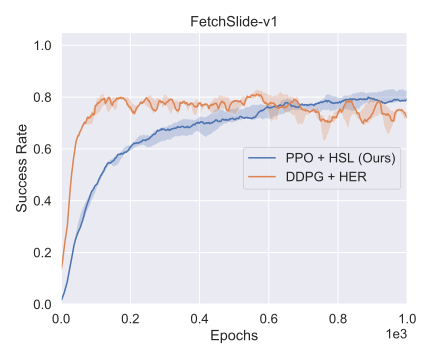
\includegraphics[width=\linewidth]{figures/chapter3/slide_her.pdf}
  ({d}) Slide
\endminipage\hfill
\caption{Results of the comparison between PPO+ESIL and DDPG+HER in all fetch tasks. \td{From the results, PPO+ESIL has worse sample efficiency than the off-policy baseline. However, PPO+ESIL achieves similar or even better performance in the end of training.}}
\label{fig:her_compare}
\end{figure}

\subsubsection{Comparison to Off-Policy Baselines}
Finally, {the proposed method is also compared} with a state-of-the-art off-policy algorithm: DDPG+HER. From {Figure~\ref{fig:her_compare}, it may be seen that} DDPG+HER converges faster than PPO+ESIL in all tasks. {However, PPO+ESIL obtains a similar performance to DDPG+HER. This is because DDPG+HER is an off-policy algorithm and uses a large number of hindsight experiences. A replay buffer is also employed to store  samples collected in the past. This approach has better sample efficiency than on-policy algorithms such as PPO.} Even so, {Figure~\ref{fig:her_compare}c} shows that PPO+ESIL still outperforms DDPG+HER in the Pick$\&$Place task and the success rate is close to 1. {This suggests that PPO+ESIL approximates the characteristics of on-policy algorithms, which have low sample efficiency, but are able to obtain a comparable performance to off-policy algorithms in continuous control tasks~\cite{schulman2017proximal}.}

\subsection{Overall Performance}
{Table~\ref{tb:ch3_last}} shows the average success rate of the last 10 epochs during training of baseline methods and PPO+ESIL. The proposed ESIL achieves the best performance in four out of five tasks. However,~PPO and PPO+SIL only obtain reasonable results in the Empty Room and Reach task. With the assistance of HER, PPO+SIL+HER obtains a better performance in the Slide task. {For the off-policy method of DDPG+HER, all five tasks are achieved, but it only obtain a better performance than PPO+ESIL in the Push task}.

\begin{table}[h]
  \centering
  \resizebox{\textwidth}{!}{
  \begin{tabular}{llllll}
    \toprule
           & {Empty Room} & {Reach} & {Push} & {Pick$\&$Place} & {Slide}  \\
    \midrule
    PPO & 1.000 $\pm$ 0.000 & 1.000 $\pm$ 0.000& 0.070 $\pm$ 0.001 & 0.033 $\pm$ 0.001 & 0.077 $\pm$ 0.001 \\
    PPO + SIL & 0.998 $\pm$ 0.002 & 0.225 $\pm$ 0.016 & 0.071 $\pm$ 0.001 & 0.036 $\pm$ 0.002 & 0.011 $\pm$ 0.001 \\
    PPO + SIL + HER &0.996 $\pm$ 0.013 & 1.000 $\pm$ 0.000 & 0.066 $\pm$ 0.011 & 0.035 $\pm$ 0.004 & 0.276 $\pm$ 0.011 \\
    DQN + HER &1.000 $\pm$ 0.000 & - & - & - & - \\
    DDPG + HER & - & 1.000 $\pm$ 0.000 & \textbf{0.996 $\pm$ 0.001} & 0.888 $\pm$ 0.008 & 0.733 $\pm$ 0.013\\
    HPG &0.964 $\pm$ 0.012 & - & - & - & - \\
    \midrule
    PPO + ESIL (Ours) & \textbf{1.000 $\pm$ 0.000} & \textbf{1.000 $\pm$ 0.000}& 0.984 $\pm$ 0.003& \textbf{0.986 $\pm$ 0.002}& \textbf{0.812 $\pm$ 0.015}\\
    \bottomrule
  \end{tabular}}
   \caption{Average success rate $\pm$ standard error in the last 10 epochs over five random seeds in all~environments {(\textbf{bold} indicates the best result among all methods).}}
  \label{tb:ch3_last}
\end{table}
% Conclusion

\section{Discussion}
\label{sec:conclusion}
This chapter proposed a novel method for self-imitation learning (SIL), in which an on-policy RL algorithm uses episodic modified trajectories, i.e., hindsight experiences, to update policies. Compared with standard self-imitation learning, episodic self-imitation learning (ESIL) has a better performance in continuous control tasks where rewards are sparse. As far as we know, it is also the first time that hindsight experiences have been combined with state-of-the-art on-policy RL algorithms, such as PPO, to solve relatively hard exploration tasks with continuous action spaces.

The experiments that we have conducted suggest that simply using self-imitation learning with the PPO algorithm, even with hindsight experience, leads to disappointing performance in continuous control Fetch tasks. In contrast, the episodic approach we take with ESIL is able to learn in these sparse reward settings. The auxiliary trajectory selection module and the adaptive weight $\beta$ help the training process to remove undesired experiences and balance the contributions to learning between the PPO term and the ESIL term automatically, and also increase the stability of training.

Our experiments suggest that the selection module is useful to prevent overfitting to sub-optimal hindsight experiences, but also that it does not always lead to learning a better policy faster. Despite~this, selection filtering appears to support learning a useful policy in challenging environments. The experiments we have conducted to date have utilised relatively small networks, and it would be appropriate to extend the experiments to consider more complex observation spaces, and to actor/critic networks, which are consequently more elaborate.

% Future work includes extending {the proposed} method to support hierarchical reinforcement learning (HRL) algorithms for more complex manipulation control tasks, such as in-hand manipulation. Episodic self-imitation learning (ESIL) can also be applied to learn sub-goal policies simultaneously.
\chapter{Efficient Sampling Strategy with Hindsight}
\label{ch:dtgsh}
\section{Introduction}
% Deep reinforcement learning (DRL)~\cite{arulkumaran2017deep}, in which neural networks are used as function approximators for reinforcement learning (RL), has been shown to be capable of solving complex control problems in several environments, including board games~\cite{schrittwieser2020mastering,silver2017mastering}, video games~\cite{berner2019dota,mnih2015human,vinyals2019grandmaster}, simulated and real robotic manipulation~\cite{andrychowicz2020learning,gu2017deep,levine2016end} and simulated autonomous driving~\cite{kiran2021deep}.

% However, learning from a \textit{sparse} reward signal, where the only reward is provided upon the completion of a task, still remains difficult. An agent may rarely or never encounter positive examples from which to learn in a sparse-reward environment. Many domains therefore provide dense reward signals~\cite{brockman2016openai}, or practitioners may turn to reward shaping~\cite{ng1999theory}. Designing dense reward functions typically requires prior domain knowledge, making this approach difficult to generalise across different environments.

% Fortunately, a common scenario is goal-oriented RL, where the RL agent is tasked with solving different goals within the same environment~\cite{kaelbling1993learning,schaul2015universal}. Even if each task has a sparse reward, the agent ideally \textit{generalises} across goals, making the learning process easier. For example, in a robotic manipulation task, the goal during a single episode would be to achieve a specific position of a target object.
In the last chapter, we have successfully combined hindsight goal relabelling with a state-of-the-art on-policy RL algorithm and introduced a new goal-oriented RL method -- episodic self-imitation learning (ESIL). Although the experiments show the effectiveness of the proposed method, ESIL still has worse sample efficiency than the vanilla hindsight experience replay (i.e., DDPG+HER). This is because DDPG is an off-policy RL algorithm, and it employs a replay buffer to store transitions during training, which enables the usage of past experiences. In this chapter, we focus on finding the shortcoming of HER and improving it to elevate learning efficiency and performance.

As a recap, hindsight experience replay (HER)~\cite{andrychowicz2017hindsight} is proposed to improve the learning efficiency of goal-oriented RL agents in sparse reward settings: when past experiences are replayed to train the agent, the desired goal is replaced (in ``hindsight'') with the achieved goal, generating many positive experiences. For example, in a robot manipulation task, the goal during a single episode would be to achieve a specific position of a target object. After applying HER, the desired target position would be overwritten with the achieved target position, with the achieved reward also being modified correspondingly.

We note that HER, whilst it enables solutions to previously unsolved tasks, can be somewhat inefficient in its use of uniformly sampling transitions during training. In the same way that prioritised experience replay~\cite{schaul2016prioritized} has significantly improved over the standard experience replay in RL, several approaches have improved upon HER by using data-dependent sampling~\cite{fang2019curriculum,zhao2018energy}. HER with energy-based prioritisation (HEBP)~\cite{zhao2018energy} assumes semantic knowledge about the goal-space and uses the energy of the target objects to sample trajectories with high energies, and then samples transitions uniformly. Curriculum-guided HER (CHER)~\cite{fang2019curriculum} samples trajectories uniformly, and then samples transitions based on a mixture of proximity to the desired goal and the diversity of the samples; CHER adapts the weighting of these factors over time. In this chapter, we introduce diversity-based trajectory and goal selection with HER (DTGSH; See Figure~\ref{fig:illustration_c4}), which samples trajectories based on the diversity of the goals achieved within the trajectory, and then samples transitions based on the diversity of the set of samples. In the experiments, DTGSH is evaluated on five challenging robot manipulation tasks. From extensive experiments, our proposed method converges faster and reaches higher rewards than prior work, without requiring domain knowledge~\cite{zhao2018energy} or tuning a curriculum~\cite{fang2019curriculum}, and is based on a single concept---determinantal point processes (DPPs)~\cite{kulesza2012determinantal}.
\begin{figure}[h]
    \centering
    \includegraphics[width=\textwidth]{figures/chapter4/illustration_DTGSH_latest.pdf}
    \caption{Overview of DTGSH. Every time a new episode is completed, its diversity is calculated, and it is stored in the episodic replay buffer. During training, $m$ episodes are sampled according to their diversity-based priority, and then $k$ diverse, hindsight-relabelled transitions are sampled using a $k$-DPP~\cite{kulesza2011k}.}
    \label{fig:illustration_c4}
\end{figure}

\section{Related Work}
The proposed work is built on HER~\cite{andrychowicz2017hindsight} as a way to effectively augment goal-oriented transitions from a replay buffer: to address the problem of sparse rewards, transitions from unsuccessful trajectories are turned into successful ones. HER uses an episodic replay buffer, with uniform sampling over trajectories, and uniform sampling over transitions. However, these samples may be redundant, and many may contribute little to the successful training of the agent.

In the literature, some efforts have been made to increase the efficiency of HER by prioritising more valuable episodes/transitions. Motivated by the work-energy principle in physics, HEBP~\cite{zhao2018energy} assigns higher probability to trajectories in which the target object has higher energy; once the episodes are sampled, the transitions are then sampled uniformly. However, HEBP requires knowing the semantics of the goal space in order to calculate the probability, which is proportional to the sum of the target's potential, kinetic and rotational energies.

CHER~\cite{fang2019curriculum} dynamically controls the sampling of transitions during training based on a mixture of goal proximity and diversity. Firstly, $m$ episodes are uniformly sampled from the episodic replay buffer, and then a minibatch of $k < m$ is sampled according to the current state of the curriculum. The curriculum initially biases sampling to achieved goals that are close to the desired goal (requiring a distance function), and later biases sampling towards diverse goals, using a $k$-nearest neighbour graph and a submodular function to more efficiently sample a diverse subset of goals (using the same distance function).

Other work has expanded HER in orthogonal directions. Hindsight policy gradient \cite{rauber2018hindsight} and episodic self-imitation learning~\cite{dai2020episodic} apply HER to improve the efficiency of goal-oriented on-policy algorithms. Dynamic HER~\cite{fang2018dher} and competitive ER~\cite{liu2018competitive} expand HER to the dynamic goal and multi-agent settings, respectively.

The use of DPPs in RL has been more limited, with applications towards modelling value functions of sets of agents in multiagent RL~\cite{osogami2019determinantal,pmlr-v119-yang20i}, and most closely related to us, finding diverse policies~\cite{parker2020effective}.

\section{Methodology}
We now formally describe the two main components of our method, DTGSH: 1) a diversity-based trajectory selection module to sample valuable trajectories for the further goal selection, and 2) a diversity-based goal selection module to select transitions with diverse goal states from the previously selected trajectories. Together, these select informative transitions from a large area of the goal space, improving the agent's ability to learn and generalise.

\subsection{Diversity-based Trajectory Selection}
We propose a diversity-based prioritisation method to select valuable trajectories for efficient training. Related to HEBP's prioritisation of high-energy trajectories~\cite{zhao2018energy}, we hypothesise that trajectories that achieve diverse goal states $g^{ac}_{t}$ are more valuable for training; however, unlike HEBP, we do not require knowledge of the goal space semantics.

In a robot manipulation task, the agent needs to move a target object from its initial position, $g^{ac}_{1}$, to the target position, $g$. If the agent never moves the object, despite hindsight relabelling it will not be learning information that would directly help in task completion. On the other hand, if the object moves a lot, hindsight relabelling will help the agent learn about meaningful interactions.

In our approach, DPPs are used to model the diversity of achieved goal states $g^{ac}_{t}$ in an episode, or subsets thereof. For a single trajectory $\Tau$ of length $T$, we divide it into several partial trajectories $\tau_{j}$ of length $b$, with achieved goal states $\{g^{ac}_{t}\}_{t=n:n+b-1}$. That is, with a sliding window of $b = 2$, a trajectory $\Tau$ can be divided into $N_p$ partial trajectories:
\begin{equation}
    \Tau_{i} = \{\{\underbrace{g^{ac}_{1}, g^{ac}_{2}}_{\tau_{1}}\}, \{\underbrace{g^{ac}_{2}, g^{ac}_{3}}_{\tau_{2}}\}, \{\underbrace{g^{ac}_{3}, g^{ac}_{4}}_{\tau_{3}}\}, \cdots, \{\underbrace{g^{ac}_{T-1}, g^{ac}_{T}}_{\tau_{N_{p}}}\}\}.
\end{equation}
The diversity $d_{\tau_{j}}$ of each partial trajectory $\tau_{j}$ can be computed as:
\begin{equation}
    d_{\tau_{j}} = \text{det}(\mathbf{L}_{\tau_{j}}), 
\label{eq:partial_div}
\end{equation}
where $\mathbf{L}_{\tau_{j}}$ is the kernel matrix of partial trajectory $\tau_{j}$:
\begin{equation}
    L_{\tau_{j}} = \mathbf{M}^{T}\mathbf{M},
\end{equation}
and $\mathbf{M}=[\hat{g}^{ac}_{n}, \hat{g}^{ac}_{n+1}, \cdots, \hat{g}^{ac}_{n+b-1}]$, where each $\hat{g}^{ac}$ is the $\ell_2$-normalised version of the achieved goal $g^{ac}$~\cite{kulesza2011k}. Finally, the diversity $d_\Tau$ of trajectory $\Tau$ is the sum of the diversity of its $N_p$ constituent partial trajectories:
\begin{equation}
    d_\Tau = \sum_{j=1}^{N_{p}} d_{\tau_{j}}.
\label{eq:total_div}
\end{equation}

Similarly to HEBP~\cite{zhao2018energy}, we use a non-uniform episode sampling strategy. During training, we prioritise sampling episodes proportionally to their diversity; the probability $p(\Tau_{i})$ of sampling trajectory $\Tau_{i}$ from a replay buffer of size $N_{e}$ is:
\begin{equation}
    p(\Tau_{i}) = \frac{d_{\Tau_{i}}}{\sum_{n=1}^{N_{e}} d_{\Tau_{n}}}.
\label{eq:diversity_priority}
\end{equation}

\subsection{Diversity-based Goal Selection}
In prior work~\cite{andrychowicz2017hindsight,zhao2018energy}, after selecting the trajectories from the replay buffer, one transition from each selected trajectory is sampled uniformly to construct a minibatch for training. However, the modified goals $g^{\prime}$ in the minibatch might be similar, resulting in redundant information. In order to form a minibatch with diverse goals for more efficient learning, we use $k$-DPPs~\cite{kulesza2011k} for sampling goals. Compared to the standard DPP, a $k$-DPP is a conditional DPP where the subset $Y$ has a fixed size $k$, with the probability distribution function:
\begin{equation}
    \mathcal{P}_{L}^{k}(\mathbf{Y}=Y) = \frac{\text{det}(\mathbf{L}_{Y})}{\sum_{|Y^{\prime}|=k} \text{det}(\mathbf{L}_{Y^{\prime}})}.
\end{equation}
$k$-DPPs are more appropriate for goal selection with a minibatch of fixed size $k$. Given $m > k$ trajectories sampled from the replay buffer, we first uniformly sample a transition from each of the $m$ trajectories. Finally, a $k$-DPP is used to sample a diverse set of transitions based on the relabelled goals $g'$ (which, in this context, we denote as ``candidate goals''). Figure~\ref{fig:goal_sampling} gives an example of uniform vs. $k$-DPP sampling, demonstrating the increased coverage of the latter. Figure~\ref{fig:kde} provides corresponding estimated density plots; note that the density of the $k$-DPP samples is actually more uniform over the \textit{support} of the candidate goal distribution.
\begin{figure}[h]
    \begin{subfigure}{\textwidth}
        \centering
        \includegraphics[width=0.9\textwidth]{figures/chapter4/goals_distribution_2d.pdf}
        \caption{Plot of candidate goals and selected goals. $k$-DPP sampling is more likely to sample points from the full span of the goal space.}
        \label{fig:goal_sampling}
    \end{subfigure}
    \begin{subfigure}{\textwidth}
        \centering
        \includegraphics[width=0.9\textwidth]{figures/chapter4/kde.pdf}
        \caption{Kernel density estimation of the distributions of goals. $k$-DPP leads to a more uniform selection of goals over the support of the goal space.}
        \label{fig:kde}
    \end{subfigure}
    \caption{Visualisation of $k=32$ goals selected from $m=100$ candidate goals of the Push task using either uniform sampling or $k$-DPP sampling, respectively. The candidate goals are distributed over a 2D ($xy$) space. Note that  $k$-DPP sampling (right hand plots) results in a broader span of selected goals in $xy$ space compared to uniform sampling (left hand plots).}
\end{figure}

% pseudo code of dpp-sampling
\begin{algorithm}[t!]
\caption{Diversity-based Goal Selection using $k$-DPP}
\label{alg:goal_sample}
\begin{algorithmic}[1]
 \REQUIRE set of $m$ candidate goal states $\mathcal{G}:=\{g_{i}\}_{i=1:m}$, minibatch size $k$
 \STATE $J \leftarrow\varnothing$, $\mathbf{M} \leftarrow  [g_{1}, g_{2}, \cdots, g_{m}]$
 \STATE Calculate the DPP kernel matrix $\mathbf{L}_\mathbf{M}$
 \STATE $\{\boldsymbol{v}_{n}, \lambda_{n}\} \leftarrow \text{EigenDecomposition}(\mathbf{L}_\mathbf{M})$
 %\STATE $e_{k}(\lambda_{1}, \cdots, \lambda_{m}): = \sum\limits_{|J'|=k}\prod_{n\in J'}\lambda_{n}$ \hfill{$\triangleright$ elementary symmetric polynomial: $e^{m}_{k}$}
 \STATE $e_k(\lambda_1,\lambda_2,\dots,\lambda_m) := 
  \sum\limits_{J^{\prime} \subseteq \{1,2,\dots,m\}\atop|J^{\prime}|=k} \prod\limits_{n \in J^{\prime}} \lambda_n$ \hfill{$\triangleright$ elementary symmetric polynomial: $e^{m}_{k}$}
 \FOR{$\mathrm{n} = m, m-1, \cdots, 1$}
 \IF{$u\sim \text{Uniform}[0, 1] < \lambda_{n}\frac{e^{n-1}_{k-1}}{e_{k}^{n}}$}
 \STATE $J \leftarrow J \cup \{n\}$, $k \leftarrow k - 1$
 \IF{$k = 0$}
 \STATE \textbf{break}
 \ENDIF
 \ENDIF
 \ENDFOR
 \STATE $V \leftarrow \{\boldsymbol{v}_{n}\}_{n \in J}$, $B \leftarrow \varnothing$
 \WHILE{$|V| > 0$}
 \STATE Select $g_{i}$ from $\mathcal{G}$ with $p(g_{i}):=\frac{1}{|V|}\sum_{\boldsymbol{v}\in V}(\boldsymbol{v}^{T}\boldsymbol{b}_{i})^{2}$\hfill{$\triangleright$ $\boldsymbol{b}_{i}$ is the $i^{\text{th}}$ standard basis}
 \STATE $B \leftarrow B \cup \{g_{i}\}$
 \STATE $V \leftarrow V_{\perp}$ \hfill{$\triangleright$ an orthonormal basis for the subspace of $V$ orthogonal to $\boldsymbol{b}_{i}$}
 \ENDWHILE
 \RETURN minibatch $B$ with size $k$
\end{algorithmic}
\end{algorithm}

\begin{algorithm}[t!]
\caption{Diversity-based Trajectory and Goal Selection with HER}
\label{alg:main_alg}
\begin{algorithmic}[1]
 \REQUIRE RL environment with episodes of length $T$, number of episodes $N$, off-policy RL algorithm $\mathbb{A}$, episodic replay buffer $\mathcal{B}$, number of algorithm updates $U$, candidate transitions size $m$, minibatch size $k$
 \STATE Initialize the parameters $\theta$ of all models in $\mathbb{A}$
 \STATE $\mathcal{B}\leftarrow\varnothing$
 \FOR{$\mathrm{i} = 1, 2, \cdots, N$}
 \STATE Sample a desired goal $g$ and an initial state $s_{0}$\hfill{$\triangleright$ start a new episode}
 \FOR{$\mathrm{t} = 1, 2, \cdots, T$}
 \STATE Sample an action $a_{t}$ using the policy $\pi(s_{t}, g;\theta)$
 \STATE Execute action $a_{t}$ and get the next state $s_{t+1}$ and achieved goal state $g^{ac}_{t+1}$
 \STATE Calculate $r_{t}$ according to Eq.~\eqref{eq:sparse_reward}
 \STATE Store transition $(s_t, a_t, r_t, s_{t+1}, g, g^{ac}_{t+1})$ in $\mathcal{B}$
 \ENDFOR
 \STATE Calculate the diversity score of current episode $d_{\Tau_{i}}$ using Eq.~\eqref{eq:partial_div} and Eq.~\eqref{eq:total_div}
 \STATE Calculate the diversity-based priority $p(\Tau)$ of each episode in $\mathcal{B}$ using Eq.~\eqref{eq:diversity_priority}
 \FOR{$\mathrm{iteration} = 1, 2, \cdots, U$}
 \STATE Sample $m$ trajectories from $\mathcal{B}$ according to priority $p(\Tau)$
 \STATE Uniformly sample one transition from each of the $m$ trajectories
 \STATE Relabel goals in each transition and recompute the reward to get $m$ candidate transitions $\{(s_{t}, a_{t}, r_{t}^{\prime}, s_{t+1}, g^{\prime})_{n}\}_{n=1:m}$
 \STATE Sample minibatch $B$ with size $k$ from the $m$ candidates using Alg.~\ref{alg:goal_sample}
 \STATE Optimise $\theta$ with minibatch $B$
 \ENDFOR
 \ENDFOR 
\end{algorithmic}
\end{algorithm}

Algorithm~\ref{alg:goal_sample} shows the details of the goal selection subroutine, and Algorithm~\ref{alg:main_alg} gives the overall algorithm for our method, DTGSH.

\section{Experiments}
We evaluate our proposed method, and compare it with current state-of-the-art HER-based algorithms~\cite{andrychowicz2017hindsight,fang2019curriculum,zhao2018energy} on challenging robot manipulation tasks~\cite{plappert2018multi}, pictured in Figure~\ref{fig:env_c4}. Furthermore, we perform ablation studies on our diversity-based trajectory and goal selection modules. Our code is based on OpenAI Baselines\footnote[1]{\url{https://github.com/openai/baselines}}, and is available at: \url{https://github.com/TianhongDai/div-hindsight}.

\begin{figure}
  \begin{subfigure}[t]{0.19\textwidth}
    \includegraphics[width=\textwidth]{figures/chapter4/push_resize.png}
    \caption{Push}
    \label{subfig:env_push}
  \end{subfigure}\hfill
  \begin{subfigure}[t]{0.19\textwidth}
    \includegraphics[width=\textwidth]{figures/chapter4/pick_resize.png}
    \caption{Pick$\&$Place}
    \label{subfig:env_pick}
  \end{subfigure}\hfill
  \begin{subfigure}[t]{0.19\textwidth}
    \includegraphics[width=\textwidth]{figures/chapter4/handegg_resize.png}
    \caption{EggFull}
    \label{subfig:env_handegg}
  \end{subfigure}\hfill
  \begin{subfigure}[t]{0.19\textwidth}
    \includegraphics[width=\textwidth]{figures/chapter4/handblock_resize.png}
    \caption{BlockRotate}
    \label{subfig:env_handblock}
  \end{subfigure}\hfill
  \begin{subfigure}[t]{0.19\textwidth}
    \includegraphics[width=\textwidth]{figures/chapter4/handpen_resize.png}
    \caption{PenRotate}
    \label{subfig:env_handpen}
  \end{subfigure}\hfill
  \caption{Robot manipulation environments. (a-b) use the Fetch robot, and (c-e) use the Shadow Dexterous Hand.} 
  \label{fig:env_c4}
\end{figure}

\subsection{Environments}
The robot manipulation environments used for training and evaluation includes five different tasks. Two tasks use the 7-DoF Fetch robot arm with two-fingers parallel gripper: Push, and Pick\&Place, which both require the agent to move a cube to the target position. The remaining three tasks use a 24-DoF Shadow Dexterous Hand to manipulate an egg, a block and a pen, respectively. The sparse reward function is given by Equation~\eqref{eq:sparse_reward}.

In the Fetch environment, the state $s_{t}$ contains the position and velocity of the joints, and the position and rotation of the cube. Each action, $a_{t}$, is a 4-dimensional vector, with three dimensions specifying the relative position of the gripper, and the final dimension specifying the state of the gripper. The desired goal $g$ is the target position, and the achieved goal $g^{ac}_{t}$ is the position of the cube. Each episode is of length $T = 50$.
%(i.e., open or closed)

In the Shadow Dexterous Hand environment, the state $s_{t}$ contains the position and velocity of the joints. Each action $a_{t}$ is a 20-dimensional vector which specifies the absolute position of 20 non-coupled joints in the hand. The desired goal, $g$, and achieved goal, $g^{ac}_t$, specify the rotation of the object for the block and pen tasks, and the position + rotation of the object for the egg task. Each episode is of length $T = 200$.

\subsection{Experimental Settings}
We base our training setup on CHER~\cite{fang2019curriculum}. We train all agents on minibatches of size $k = 64$ for 50 epochs using MPI for parallelisation over 16 CPU cores; each epoch consists of 1600 ($16 \times 100$) episodes, with evaluation over 160 ($16 \times 10$) episodes at the end of each epoch. Remaining hyperparameters for the baselines are taken from the original respective works~\cite{andrychowicz2017hindsight,fang2019curriculum,zhao2018energy}. Our method, DTGSH, uses partial trajectories of length $b = 2$ and $m = 100$ as the number of candidate goals. 


\subsection{Results on Benchmark Environments}
We compare DTGSH to DDPG~\cite{lillicrapContinuous}, DDPG+HER~\cite{andrychowicz2017hindsight}, DDPG+HEBP~\cite{zhao2018energy} and DDPG+\\CHER~\cite{fang2019curriculum}. Evaluation results are given based on repeated runs with 5 different seeds; we plot the median success rate with upper and lower bounds given by the \nth{75} and \nth{25} percentiles, respectively.

\begin{figure}
\centering
  \begin{subfigure}[t]{0.49\textwidth}
    \includegraphics[width=\textwidth]{figures/chapter4/FetchPush-v1.pdf}
    \caption{Push}
    \label{subfig:baseline_push}
  \end{subfigure}\hfill
  \begin{subfigure}[t]{0.49\textwidth}
    \includegraphics[width=\textwidth]{figures/chapter4/FetchPickAndPlace-v1.pdf}
    \caption{Pick\&Place}
    \label{subfig:baseline_pick}
  \end{subfigure}\hfill
  \begin{subfigure}[t]{0.49\textwidth}
    \includegraphics[width=\textwidth]{figures/chapter4/HandManipulateEggFull-v0.pdf}
    \caption{EggFull}
    \label{subfig:baseline_handegg}
  \end{subfigure}\hfill
  \begin{subfigure}[t]{0.49\textwidth}
    \includegraphics[width=\textwidth]{figures/chapter4/HandManipulateBlockRotateXYZ-v0.pdf}
    \caption{BlockRotate}
    \label{subfig:baseline_handblock}
  \end{subfigure}\hfill
  \begin{subfigure}[t]{0.49\textwidth}
    \includegraphics[width=\textwidth]{figures/chapter4/HandManipulatePenRotate-v0.pdf}
    \caption{PenRotate}
    \label{subfig:baseline_handpen}
  \end{subfigure}\hfill
%   \begin{subfigure}[t]{0.49\textwidth}
%     \includegraphics[width=\textwidth]{figures/chapter4/blank.png}
%   \end{subfigure}\hfill
  \caption{Success rate of DTGSH and baseline approaches. \td{DDPG+DTGSH outpeforms other baselines in all tasks, and without using HER, DDGP cannot even complete the simple Reach task.}} 
  \label{fig:baseline_compare_c4}
\end{figure}

Figure~\ref{fig:baseline_compare_c4} and Table~\ref{tab:benchmark} show the performance of DDPG+DTGSH and baseline approaches on all five tasks. In the Fetch tasks, DDPG+DTGSH and DDPG+HEBP both learn significantly faster than the other methods, while in the Shadow Dexterous Hand tasks DDPG+DTGSH learns the fastest and achieves higher success rates than all other methods. In particular, DDPG cannot solve any tasks without using HER, and CHER performs worse in the Fetch tasks. We believe the results highlight the importance of sampling both diverse trajectories \textit{and} goals, as in our proposed method, DTGSH.
\begin{table}[h]
    \centering
    \resizebox{\textwidth}{!}{
    \begin{tabular}{c|c@{\hskip 0.1in}|c@{\hskip 0.1in}|c|c|c}
    \toprule
         & Push & Pick\&Place & EggFull & BlockRotate & PenRotate \\
        \midrule
        DDPG & 0.09$\pm$0.01 & 0.04$\pm$0.00 & 0.00$\pm$0.00 & 0.01$\pm$0.00 & 0.00$\pm$0.00 \\
        DDPG+HER & \textbf{1.00$\pm$0.00} & 0.89$\pm$0.03 & 0.11$\pm$0.01 & 0.55$\pm$0.04 & 0.15$\pm$0.02 \\
        DDPG+HEBP & \textbf{1.00$\pm$0.00} & 0.91$\pm$0.03 & 0.14$\pm$0.02 & 0.59$\pm$0.02 & 0.20$\pm$0.03\\
        DDPG+CHER & \textbf{1.00$\pm$0.00} & 0.91$\pm$0.04 & 0.15$\pm$0.01 & 0.54$\pm$0.04 & 0.17$\pm$0.03 \\
        \midrule
        DDPG+DTGSH & \textbf{1.00$\pm$0.00} & \textbf{0.94$\pm$0.01} & \textbf{0.17$\pm$0.03} & \textbf{0.62$\pm$0.02} & \textbf{0.21$\pm$0.02}\\
        \bottomrule
    \end{tabular}
    }
    \vspace{0.2em}
    \caption{Final mean success rate $\pm$ standard deviation, with best results in \textbf{bold}.}
    %\vspace{-14mm}
    \label{tab:benchmark}
\end{table}
%\vspace{-15mm}
\subsection{Results on Ablation Studies}
In this section, we perform the following experiments to investigate the effectiveness of each component in DTGSH: 1) diversity-based trajectory selection with HER (DTSH) and diversity-based goal selection with HER (DGSH) are evaluated independently to assess the contribution of each stage, 2) the performance using different partial trajectory lengths $b$, and 3) the performance of using different candidate goal set sizes $m$.
\begin{figure}[h!]
  \centering
  \begin{subfigure}[t]{0.49\textwidth}
    \includegraphics[width=\textwidth]{figures/chapter4/FetchPush-v1_ab1.pdf}
    \caption{Push}
    \label{subfig:baseline_push_ab1}
  \end{subfigure}\hfill
  \begin{subfigure}[t]{0.49\textwidth}
    \includegraphics[width=\textwidth]{figures/chapter4/FetchPickAndPlace-v1_ab1.pdf}
    \caption{Pick\&Place}
    \label{subfig:baseline_pick_ab1}
  \end{subfigure}\hfill
  \begin{subfigure}[t]{0.49\textwidth}
    \includegraphics[width=\textwidth]{figures/chapter4/HandManipulateEggFull-v0_ab1.pdf}
    \caption{EggFull}
    \label{subfig:baseline_handegg_ab1}
  \end{subfigure}\hfill
  \begin{subfigure}[t]{0.49\textwidth}
    \includegraphics[width=\textwidth]{figures/chapter4/HandManipulateBlockRotateXYZ-v0_ab1.pdf}
    \caption{BlockRotate}
    \label{subfig:baseline_handblock_ab1}
  \end{subfigure}\hfill
  \begin{subfigure}[t]{0.49\textwidth}
    \includegraphics[width=\textwidth]{figures/chapter4/HandManipulatePenRotate-v0_ab1.pdf}
    \caption{PenRotate}
    \label{subfig:baseline_handpen_ab1}
  \end{subfigure}\hfill
%   \begin{subfigure}[t]{0.33\textwidth}
%     \includegraphics[width=\textwidth]{figures/chapter4/blank.png}
%   \end{subfigure}\hfill
  \caption{Success rate of HER, DTGSH, and ablations DTSH and DGSH. \td{From the results, DTSH outperforms DDPG+HER in all tasks, which verify the efficiency that selecting trajectories with diverse achieved goals for training. DGSH also has better performance than DDPG+HER in three tasks. By combining these two modules together, DTGSH achieves the best performance.} } 
  \label{fig:ablation1}
\end{figure}

Figure~\ref{fig:ablation1} shows the performance of using DTSH and DGSH independently. DDPG+\\DTSH outperforms DDPG+HER substantially in all tasks, which supports the view that sampling trajectories with diverse achieved goals can substantially improve performance. Furthermore, unlike DDPG+HEBP, DTSH does not require knowing the structure of the goal space in order to calculate the energy of the target object; DDPG+DGSH achieves better performance than DDPG+HER in three tasks, and is only worse in one task. DGSH performs better in the environment where it is easier to solve the task (e.g., Fetch tasks), and hence the trajectories selected are more likely to contain useful transitions. However, DTGSH, which is the combination of both modules, performs the best overall.

\begin{figure}[h!]
\centering
  \begin{subfigure}[t]{0.49\textwidth}
    \includegraphics[width=\textwidth]{figures/chapter4/FetchPush-v1_ab2.pdf}
    \caption{Push}
    \label{subfig:baseline_push_ab2}
  \end{subfigure}\hfill
  \begin{subfigure}[t]{0.49\textwidth}
    \includegraphics[width=\textwidth]{figures/chapter4/FetchPickAndPlace-v1_ab2.pdf}
    \caption{Pick\&Place}
    \label{subfig:baseline_pick_ab2}
  \end{subfigure}\hfill
  \begin{subfigure}[t]{0.49\textwidth}
    \includegraphics[width=\textwidth]{figures/chapter4/HandManipulateEggFull-v0_ab2.pdf}
    \caption{EggFull}
    \label{subfig:baseline_handegg_ab2}
  \end{subfigure}\hfill
  \begin{subfigure}[t]{0.49\textwidth}
    \includegraphics[width=\textwidth]{figures/chapter4/HandManipulateBlockRotateXYZ-v0_ab2.pdf}
    \caption{BlockRotate}
    \label{subfig:baseline_handblock_ab2}
  \end{subfigure}\hfill
  \begin{subfigure}[t]{0.49\textwidth}
    \includegraphics[width=\textwidth]{figures/chapter4/HandManipulatePenRotate-v0_ab2.pdf}
    \caption{PenRotate}
    \label{subfig:baseline_handpen_ab2}
  \end{subfigure}\hfill
%   \begin{subfigure}[t]{0.33\textwidth}
%     \includegraphics[width=\textwidth]{figures/chapter4/blank.png}
%   \end{subfigure}\hfill
  \caption{Success rate of DTGSH with different partial trajectory lengths $b$ and different candidate goal set sizes $m$. \td{From the results, when $b \gg 2$, the performance degrades in all tasks. When $m \gg 100$, the performance degrades in the Shadow Dexterous Hand environment.}} 
  \label{fig:ablation2}
\end{figure}

Figure~\ref{fig:ablation2} shows the performance of DDPG+DTGSH with different partial trajectory lengths $b$ and different candidate goal set sizes $m$. In this work, we use $b = 2$ and $m = 100$ as the defaults. Performance degrades with $b \gg 2$, indicating that pairwise diversity is the best for learning in our method. $m \gg 100$ does not affect performance in the Fetch environment, but degrades performance in the Shadow Dexterous Hand environment.

\subsection{Time Complexity}
Table~\ref{tab:time} gives example training times of all of the HER-based algorithms. DTGSH requires an additional calculation of the diversity score of $\mathcal{O}(N_{p}b^3)$ at the end of every training episode, and sampling of $\mathcal{O}(mk^2)$ for each minibatch.
\begin{table}[h!]
    \centering
    \resizebox{0.85\textwidth}{!}{
    \begin{tabular}{c|c|c|c|c}
    \toprule
           & DDPG+HER & DDPG+HEBP & DDPG+CHER & DDPG+DTGSH\\
        \midrule
        Time  & 00:55:08 & 00:56:32 & 03:02:18 & 01:52:30 \\
        \bottomrule
    \end{tabular}
    }
    \vspace{0.2em}
    \caption{Training time (hours:minutes:seconds) of DTGSH and baseline approaches on the Push task for 50 epochs.}
    \label{tab:time}
\end{table}

\section{Discussion}
In this chapter, we introduced diversity-based trajectory and goal selection with hindsight experience replay (DTGSH) to improve the learning efficiency of goal-orientated RL agents in sparse reward settings. Our method can be divided into two stages: 1) valuable trajectories are selected according to diversity-based priority, as modelled by determinantal point processes (DPPs)~\cite{kulesza2012determinantal}, and 2) $k$-DPPs~\cite{kulesza2011k} are leveraged to sample transitions with diverse goal states from previously selected trajectories for training. Our experiments empirically show that DTGSH achieves faster learning and higher final performance in five challenging robot manipulation tasks, compared to previous state-of-the-art approaches~\cite{andrychowicz2017hindsight,fang2019curriculum,zhao2018energy}. Furthermore, unlike prior extensions of hindsight experience replay, DTGSH does not require semantic knowledge of the goal space~\cite{zhao2018energy}, and does not require tuning a curriculum~\cite{fang2019curriculum}.
\newcommand{\ourmethod}{\text{DAIM}}
\newcommand{\policypi}{\mathbf{\pi} }
\newcommand{\expection}{\mathbb{E} }
\newcommand{\tables}{{Table }}
\newcommand{\eq}{{Equation }}
\newcommand{\alg}{{Algorithm }}
\newcommand{\starcraft}{{StarCraft II}}

\chapter{Diversity-Augmented Intrinsic Motivation}
\label{ch:daim}
\section{Introduction}
In order to improve sample efficiency of DRL algorithms in the environments offering sparse rewards, Chapter~\ref{ch:esil} proposes a novel self-imitation loss function to increase the frequency that the agent achieves positive samples, and Chapter~\ref{ch:dtgsh} uses the determinantal point processes (DPPs) framework to measure the diversity of achieved goals in a trajectory and proposes a sampling strategy that uses diversity as a priority to sample the trajectories for further processing, in which diversity can also quantify the contribution of each trajectory. In this chapter, we keep exploring the potential application of determinantal point processes (DPPs) in deep reinforcement learning (DRL). In contrast to previous chapters, DPPs are used to quantify the discrepancy between adjacent states as additional endogenous rewards to accelerate the training of DRL agents in the environment with the sparse reward setting.

%Deep reinforcement learning (RL) allows agents to learn a wide range of reward-driven skills, including playing games~\cite{mnih2015human,silver2016mastering,xu2020neurips}, controlling robots~\cite{dai2020episodic,fang2018dher,gu2017deep,levine2016end}, and making decisions in other environments~\cite{fang2017learning,vinyals2017starcraft}. 

%Many significant application problems in DRL can be formulated as a 
% Many important applied problems in DRL can be accurately modelled as learning from extrinsic rewards, where a function (approximately) relates features associated with a state/action pair and the expectation of the resulting rewards. Furthermore, with appropriate features, it is often the case that linear or nonlinear functions can accurately approximate the reward function. However, hand-crafted reward functions usually lead to unexpected behaviors~\cite{riedmiller2018learning} and limited exploration. 
% Potential-based reward shaping methods~\cite{ng1999policy} offers a general answer to what degree of reward function modifications do not affect the optimal policy. Other works have tried to design auxiliary rewards to derive policies with desired properties. For example, Jaderberg \textit{et al.}~\cite{jaderberg2016reinforcement} calculate a pseudo-reward from unsupervised auxiliary tasks, and use this reward to refine its internal representation. In count-based methods~\cite{bellemare2016unifying, ostrovski2017count, tang2017exploration}, a pseudo-count based reward is used to encourage the agent to explore novel states in the environment.

% In environments or tasks for which the reward sparsity is higher, undirected, or even deceptive, the application of RL techniques is significantly more difficult, since the agent might have only occasional opportunities to improve its policy, such as when the final goal is reached. In such scenarios, agents can be endowed with mechanisms of {\it intrinsic motivation} that encourage exploration in environments and learn useful policies even without explicit supervision. Early attempts to incorporate intrinsic motivation use self-supervised prediction errors as intrinsic rewards to help the agent explore~\cite{pathak2017curiosity}. More recently, Zheng \textit{et al.}~\cite{zheng2018learning} design an augmented agent with additive intrinsic rewards. When the intrinsic value of the action is added to the task-dependent (i.e., extrinsic) rewards, the performance of policy gradient based learning methods can be improved. 
%Another line of work uses auxiliary control tasks, such as pixel control or feature control, which can significantly speed up learning of the main task. The rationale is that learning the auxiliary tasks gives the agent features that are useful for manipulating the environment. However, these intrinsic methods are either difficult to explain or only specific to some tasks.

Encouraging the agent to explore previously unseen/novel states in the environments with sparse or delayed reward settings is still a challenge in DRL. In this chapter, we demonstrate how a simple generated intrinsic reward function based on a diversity measure can enable RL agents to explore novel states efficiently. This generated auxiliary reward is functional for a number of environments, as confirmed by a selection of MuJoCo locomotion tasks and video games.

% Encouraging effective exploration of novel states for agents without any reward signal is still a challenging problem. Making progress on this problem requires specifying a learning objective that ensures the agent explores large parts of the state space. In this chapter, we demonstrate how a simple generated intrinsic reward function based on a diversity measure can enable RL agents to explore novel states efficiently. This auxiliary reward is functional for a number of environments, as confirmed by a selection of MuJoCo locomotion tasks and video games.

%We hypothesise that in order to acquire an agent that is useful and efficient, we must train the agent so that it can attain coverage over the set of possible states.

In order to obtain an agent that can solve the tasks with sparse or delayed rewards, we need the agent to explore as many novel states as possible during training. However, common exploration strategies ({e.g.}, random sampling, $\epsilon$-greedy) can re-visit previously explored states in the environment, which can limit the effectiveness of state-space coverage.

A key idea in our work is to use a measure of discrepancy between states as an intrinsic motivation. To model the diversity of the agent's states, we adopt the framework of determinantal point processes (DPPs)~\cite{kulesza2012determinantal} to formulate the intrinsic reward as a dynamic measure of diversity. Regarding the sequence of states as a DPP allows a measure of the diversity of subset selection, widely used in data summarization for selecting a diversified subset~\cite{gong2014diverse}. We build an intrinsic reward for diversity with parameterised DPPs and propose a new general method for learning policies with intrinsic rewards. The proposed method is referred to as diversity-augmented intrinsic motivation ($\ourmethod$). Through a series of experiments, we show that the agents trained with the proposed diversity-based intrinsic rewards learn effectively and attain higher rewards than well-known baselines, especially in continuous control environments.

The contributions of this chapter can be summarized as follows: 1) The DPPs framework is proposed as a measure for the diversity of adjacent states, and this diversity is used as the intrinsic reward, 2) A bi-level optimisation~\cite{zheng2018learning} is borrowed to combine with the proposed diversity-based measure, so that the intrinsic reward will increase the extrinsic reward while increasing diversity, and 3) $\ourmethod$ is evaluated in the MuJoCo locomotion and arcade learning environments. Empirical results demonstrate that $\ourmethod$ can outperform baseline methods in most of the standard tasks and outperform baselines in 12 out of 15 tasks with delayed rewards in the MuJoCo locomotion environment. In addition, $\ourmethod$ also improves the rate of learning in the initial stage of training in the arcade learning environment.
\newpage

\section{Related Work}
Intrinsic motivation is an approach to explore novel states which may lead to higher rewards in the future. Pathak \textit{et al.}~\cite{pathak2017curiosity} propose an intrinsic curiosity module (ICM), suggesting the prediction error between an actual encoded frame and the predicted encoded frame as the intrinsic reward. A higher prediction error indicates the agent has moved into a novel state, and this intrinsic reward will encourage the agent to keep exploring such novel states. In order to find an appropriate representation of pixels that could be invariant to insignificant changes in the environment, an inverse dynamic model is introduced to extract features. This requires training a network, which uses consecutive frames as input to predict the action that would transition the previous frame to the subsequent. The insight of the inverse dynamic model is that through predicting environment dynamics, features are learned to preserve the key information that predicts the action. Burda \textit{et al.}~\cite{burda2018largescale} conduct a large-scale study of curiosity-driven learning. Their findings suggest that an agent can learn to play a significant number of Atari games, even without receiving any extrinsic rewards from the environment. 

However, environments with stochastic dynamics may not be suitable for the application of purely exploratory approaches. Variational Information Maximising Exploration (VIME)~\cite{NIPS2016_abd81528} formulates the intrinsic reward based on the information gain according to the agent’s belief of environment dynamics, and it shows significant improvements in the continuous control tasks with the sparse reward setting. 

Zheng \textit{et al.}~\cite{zheng2018learning} introduce learning intrinsic reward for policy gradient (LIRPG), which enables a learnable intrinsic reward function to be used for training an RL agent. In addition, LIRPG adopts a bi-level optimisation scheme that when the policy network is updated to maximise the accumulated intrinsic and extrinsic rewards, the intrinsic reward function is also updated to maximise the accumulated extrinsic rewards achieved by the policy network. This optimisation scheme guarantees the learned reward function can generate meaningful intrinsic rewards to facilitate the agent reaching the ultimate goal (i.e., maximising the accumulated extrinsic rewards). In this work, we also leverage this bi-level optimisation to ensure the agent can explore novel states that deliver more accumulated extrinsic rewards.

\section{Methodology}
% start
\begin{figure}[t]
    \centering
    \includegraphics[width=\linewidth]{figures/chapter5/illustration.pdf}
    \caption[Illustration of $\ourmethod$.]{Illustration of $\ourmethod$. It shows the intrinsic rewards of an entire episode of SuperMarioBros. The red points annotate the key frames in the game. In frames \{17, 26, 32, 41\}, the agent keeps moving forward, and the intrinsic rewards are relatively higher. In the frames \{303, 327, 354, 379\}, the agent is stuck at the bottom of the flagpole. For these latter four frames, the diversity between adjacent states is very small, and the intrinsic rewards are close to zero.}
    \label{fig:illustration}
\end{figure}

In the proposed method, let $r_{t}^{\text{ex}}$ denote the extrinsic reward received from the environment and $r^{\text{in}}_{t}$ denote the intrinsic reward parameterised by $\eta$. The agent can receive a mixed reward represented in the following form:
\begin{equation}
    r^{\text{mix}}_t = \lambda^{\text{ex}} r^{\text{ex}}(s_{t}, a_t) + \lambda^{\text{in}} r^{\text{in}}(s_t, s_{t+1};\eta),
\end{equation}
where $\lambda^{\text{ex}}$ and $\lambda^{\text{in}}$ are the weight coefficients of the extrinsic reward $r^{\text{ex}}_{t}$ and the intrinsic reward $r^{\text{in}}_{t}$ at timestep $t$. The agent is updated to maximise the diversity-augmented return $G^{\text{mix}}(s_t,a_t)$, where $G^{\text{mix}}(s_t,a_t) =\sum_{k=0}^{T-1}\gamma^{k}r^{\text{mix}}_{t+k}$. Notice that the ultimate goal of the agent is still maximising the extrinsic return $G^{\text{ex}}(s_{t}, a_{t})$. 

In the rest of this section, we first introduce the primary objective function and the optimisation algorithm that can ensure the maximisation of the extrinsic return while increasing the diversity-augmented returns. Subsequently, the intrinsic reward formulated under the DPPs framework is discussed.

\subsection{Primary Objective Function}
To make sure that $\ourmethod$ still increases the extrinsic reward, we adopt a bi-level optimisation framework. The objective function is defined as follows:
\begin{align}
  \label{eq:obj}
  \max_{\eta}\quad & J^{\text{ex}}(\eta;\theta^{\prime}),\\ 
  \text{subject to}\quad & \theta^{\prime} =\mathop{\arg\max}_{\theta}\ J^{\text{mix}}(\theta, \eta).
  \nonumber
\end{align}
Here $J^{\text{mix}} = \mathbb{E}_{\pi_{\theta}}\bigr[G^{\text{mix}}(s_t,a_t) \bigr]$, and $\theta$ represents the parameters of the policy network.
The optimisation problem of \eqref{eq:obj} can be viewed as a bi-level optimisation, which is widely used in the fields of machine learning, such as meta-learning~\cite{andrychowicz2016learning,nichol2018first,santoro2016meta,xu2018meta,zheng2018learning}, signal processing~\cite{kunapuli2008classification,flamary2014learning}, and hyperparameters optimisation~\cite{franceschi2018bilevel, shaban2019truncated}. In Equation~\eqref{eq:obj}, $J^{\text{ex}}$ and $J^{\text{mix}}$ are upper-level and lower-level objective functions, respectively. The primary goal of this bi-level objective function is to maximise extrinsic returns (upper-level objective function) $J^{\text{ex}}$ with respect to the parameters of intrinsic reward $\eta$, and the updated parameters of the policy network $\theta^{\prime}$ can be achieved via maximising the lower-level objective function.

% The upper-level optimisation is treated as the leader, while the lower-level optimisation is the follower. The upper agent reshapes the reward to make the low-level agent's learning easier. The low-level agent observes the commands of the upper-level agent and works towards meeting the commands.

The policy parameters $\theta$ and the intrinsic parameters $\eta$ can be updated alternately.
Firstly, the update of the policy network $\pi_{\theta}$ with a learning rate $\alpha$ can be written as:
\begin{equation}
    \theta^{\prime}=\theta + \alpha\nabla_{\theta} \log \pi(a_t|s_t;\theta)G^{\text{mix}}(s_t, a_t).
\label{eq:mix_cost}
\end{equation}
Secondly, we update $\eta$ towards maximising the expected extrinsic returns $G^{\text{ex}}(s_t, a_t)$ of the agent. 
To build the connection between $J^{\text{ex}}$ and $\eta$, the updated parameters of the policy network $\theta^{\prime}$ are used to sample a new trajectory and solve the following problem:
\begin{equation}
    \max_{\eta} J^{\text{ex}} = \mathbb{E}_{\pi_{\theta^{\prime}|\eta}}[G^{\text{ex}}(s_t, a_t)].
\label{eq:cost_ex}
\end{equation}
Then, the gradient $\nabla_{\eta} J^{\text{ex}}$ can be calculated using the chain rule:
\begin{equation}
    \nabla_{\eta} J^{\text{ex}} = \nabla_{\theta^{\prime}}J^{\text{ex}}\nabla_{\eta}\theta^{\prime}, 
  \label{eq:chain_rule}
\end{equation}
with 
\begin{align}
    \nabla_{\eta}\theta^{\prime} &=  \nabla_{\eta}\alpha G^{\text{mix}}(s_t, a_t) \nabla_{\theta} \log \pi(a_t|s_t;\theta) \nonumber \\
    &= \alpha\lambda^{\text{in}}\sum_{k=0}^{\infty}\gamma^{k}\nabla_{\eta}r^{\text{in}}_{\eta,t+k}\nabla_{\theta} \log \pi(a_t|s_t;\theta). 
\end{align}

Here, instead of collecting another set of samples, importance sampling is employed to increase the sample efficiency of the algorithm:
\begin{equation}
    \nabla_{\theta^{\prime}}J^{\text{ex}} =  \nabla_{\theta^{\prime}}\Bigg (\frac{\pi(a_{t}|s_{t};\theta^{\prime})}{\pi(a_{t}|s_{t};\theta)}\Bigg ) G^{\text{ex}}(s_{t}, a_{t}).
\label{eq:importance_sampling}
\end{equation}
% The principle of the \eq \eqref{eq:chain_rule} is to formulate the effect of the change of $\eta$ on influencing $J^{\text{ex}}$ through its influence on the updated policy parameter $\theta'$.
%This is a commonly adopted technique in meta-gradient learning~\cite{andrychowicz2016learning,nichol2018first,santoro2016meta,xu2018meta,zheng2018learning}. 
Through this bi-level optimisation, the features that are learned ensure that the resulting diversity also increases the extrinsic returns. Furthermore, the value network is updated via a mean squared error loss $\mathcal{L}_{value} = \mathbb{E}[(V(s_{t};\psi) - G_{t}^{\text{mix}})^2]$. Algorithm~\ref{algo:vi} gives the pseudo code for our method -- diversity-augmented intrinsic motivation ($\ourmethod$). The code is publicly available at: \url{https://github.com/TianhongDai/daim-rl}.

\begin{algorithm}[t]
	\caption{\label{alg:all} Diversity-Augmented Intrinsic Motivation.
	}
	\begin{algorithmic}[1]
		\REQUIRE a policy network $\pi(a_{t}|s_{t};\theta)$, an intrinsic reward module $\phi(s_{t},s_{t+1};\eta)$, a value network $V(s_{t};\psi)$, learning rate $\alpha$, intrinsic module learning rate $\beta$, transition buffer $\mathcal{B}$, number of iterations $N$, length of each rollout $T$, weight coefficient of extrinsic reward $\lambda^{\text{ex}}$, weight coefficient of intrinsic reward $\lambda^{\text{in}}$
		%\STATE \textbf{Init}: initialize the policy network $\pi(a_{t}|s_{t};\theta)$ and intrinsic network $\phi(s_{t};\eta)$
		\FOR{iteration = 1, 2, 3, ..., $N$}
		\STATE Let $\mathcal{B} \leftarrow \varnothing$
		\FOR{$t$ = 1, 2, 3, ..., $T$}
        \STATE Sample an action $a_{t}$ using policy network $\pi(a_{t}|s_{t};\theta)$
        \STATE Execute the action $a_{t}$ and get the next state $s_{t+1}$ and the extrinsic reward $r^{\text{ex}}_{t}$
		\STATE Calculate the kernel matrix: $\textbf{L}_{y}=\mathbf{M}^{T}\mathbf{M}$ using $\phi(s_{t},s_{t+1};\eta)$
		\STATE Compute the intrinsic reward: $r_{t}^{\text{in}} = \det\left(\mathbf{L}_{y} \odot \left(\diag{(\mathbf{L}_{y}})^{T}\diag({\mathbf{L}_{y}})\right)^{-\frac{1}{2}}\right)$
		\STATE Store the transition $(s_{t}, r^{\text{in}}_{t}, r^{\text{ex}}_{t}, s_{t+1}, a_{t})$ in $\mathcal{B}$
		\ENDFOR
		\STATE Compute the diversity-augmented return $G^{\text{mix}}(s, a)$ using the mixed reward: $r^{\text{mix}}=\lambda^{\text{ex}}r^{\text{ex}} + \lambda^{\text{in}}r^{\text{in}}$
		\STATE Compute the extrinsic return $G^{\text{ex}}(s, a)$ using the extrinsic reward: $r^{\text{ex}}$
		\STATE Update $\theta$ according to Eq.\eqref{eq:mix_cost} with learning rate $\alpha$
		\STATE Update $\psi$ according to $\mathcal{L}_{value}=\mathbb{E}[(V(s_{t};\psi)-G^{\text{mix}}_{t})^2]$ with learning rate $\alpha$
		\STATE Update $\eta$ according to Eq.\eqref{eq:chain_rule} and Eq.\eqref{eq:importance_sampling} with learning rate $\beta$
        \ENDFOR
	\end{algorithmic}
	\label{algo:vi}
\end{algorithm}
\subsection{Parameterised Diversity as Intrinsic Reward}
We are now able to parameterise the intrinsic reward with parameter $\eta$ in this section. The intrinsic reward at timestep $t$ is defined as:
\begin{equation}
    r^{\text{in}}(s_t, s_{t+1}; \eta) = \det\left(\mathbf{L}_{{y}=\{s_{t},s_{t+1}\}}\right),
\label{eq:intrinsic}
\end{equation}
where $\mathbf{L}_{y}$ is the kernel matrix of the subset $y=\{s_{t}, s_{t+1}\}$ with:
\begin{equation}
    \mathbf{L}_{y} = \mathbf{M}^{T}\mathbf{M},
\label{eq:kernel_matrix}
\end{equation}
and $\mathbf{M} = [\phi(s_{t};\eta),\phi(s_{t+1};\eta)]$ and $\phi(\cdot;\eta)$ is the feature vector parameterised by the intrinsic parameter $\eta$.
$r_{t}^{\text{in}}$ measures the diversity of the adjacent state sequence ${y}=\{s_{t},s_{t+1}\}$. Intuitively, it represents the diversity that an action, $a_t$, will bring to the trajectory. In order to scale the intrinsic reward, $r^{\text{in}}_{t}$, in a reasonable range ({e.g.}, [0, 1]), the kernel matrix $\mathbf{L}_{y}$ can be normalised by:
\begin{equation}
    \mathbf{L}_{y}^{\prime} = \mathbf{L}_{y} \odot \left(\diag{(\mathbf{L}_{y}})^{T}\diag({\mathbf{L}_{y}})\right)^{-\frac{1}{2}},
\end{equation}
where $\odot$ is the element-wise multiplication and $\diag(\cdot)$ outputs the diagonal elements of $\mathbf{L}_{y}$ as a vector. 

Figure~\ref{fig:illustration} illustrates the proposed intrinsic reward. When the agent is moving ahead (e.g., timesteps $\in$[10, 200]), the intrinsic rewards are higher than when the agent is stuck. In contrast, when the agent is stuck at the bottom of the flagpole, the intrinsic rewards are close to zero (e.g., timesteps $\in$[250, 380]). Figure~\ref{fig:structure_overview} shows the overview of three networks used in DAIM.

\begin{figure}[h]
    \centering
    \includegraphics[width=0.7\linewidth]{figures/chapter5/daim-struct.pdf}
    \caption[Overview of three networks in DAIM.]{Overview of three networks in DAIM: intrinsic reward module, policy network, and value network.}
    \label{fig:structure_overview}
\end{figure}

\section{Experiments}
In this section, we evaluate $\ourmethod$ with different selections of baseline policy gradient architecture, namely, proximal policy optimisation (PPO) and advantage actor critic (A2C). We choose MuJoCo locomotion and the arcade learning environments (Atari games and SuperMarioBro) as the benchmark environments (see Figure~\ref{fig:ch5_envs}).
\begin{figure}[h]
    \begin{subfigure}{\textwidth}
        \centering
        \includegraphics[width=0.9\textwidth]{figures/chapter5/mujoco_env.pdf}
        \caption{MuJoCo Locomotion Environment.}
        \label{fig:mujoco_env}
    \end{subfigure}
    \begin{subfigure}{\textwidth}
        \centering
        \includegraphics[width=0.9\textwidth]{figures/chapter5/atari_env.pdf}
        \caption{Arcade Learning Environment.}
        \label{fig:ale_env}
    \end{subfigure}
    \caption[Evaluation environments of DAIM.]{Visualisation of (a) MuJoCo Locomotion Environment: HalfCheetah, Hopper, Walker2d, Ant, and Humanoid, and (b) Arcade Learning Environment: Alien, BeamRider, Breakout, MsPacman, UpNDown, and SuperMarioBros.}
    \label{fig:ch5_envs}
\end{figure}

\subsection{Environments}
Firstly, we evaluate our agent in the MuJoCo locomotion environment~\cite{duan2016benchmarking} and use PPO as the base RL algorithm. We use two kinds of environment settings for evaluation: the standard setting and the delayed reward setting~\cite{zheng2018learning}. Specifically, {for the delayed reward setting}, the accumulated reward is only given every 10, 20 or 40 steps. This setting is more difficult for agent learning. The five tasks selected in the experiment are HalfCheetah, Hopper, Walker2d, Ant and Humanoid (see Figure~\ref{fig:mujoco_env}).

Subsequently, to investigate the performance of $\ourmethod$ with high dimensional inputs, we also evaluate our approach on the Atari games and the SuperMarioBros~\cite{gym-super-mario-bros} using A2C as our base RL algorithm. For the Atari games, Alien, BeamRider, Breakout, MsPacman and UpNDown are selected as our test bench (see Figure~\ref{fig:ale_env}). 

\subsection{Experimental Settings}
In MuJoCo tasks, baseline methods are vanilla PPO~\cite{schulman2017proximal}, LIRPG~\cite{zheng2018learning} and VIME~\cite{NIPS2016_abd81528}. The intrinsic module $\phi_{\eta}(\cdot)$ has 3 hidden layers with 64 neurons with ReLU activation functions. The output of the intrinsic module is a 64 dimensional embedding feature. Adam~\cite{kingma2014adam} is chosen as the optimiser with learning rate $\alpha=0.0001$. $\lambda^{\text{in}}$ and $\lambda^{\text{ex}}$ are both set to 1 as default. The hyperparameters of PPO part are kept the same as the baseline setting: timesteps per rollout are 2048, clip ratio is 0.2, entropy coefficient is 0, optimisation epochs per iteration is 10, batch size is 64, learning rate is 0.0003, discount factor $\gamma$ is 0.99, and GAE parameter $\lambda$ is 0.95. Training for each agent lasts for 1 million frames. {The average time of one complete training run of DAIM using one random seed on the MuJoCo tasks is 1.46 hours.}

In the Atari games and SuperMarioBros, Vanilla A2C and LIRPG are selected as baseline methods. For $\ourmethod$, the same CNN architecture as A2C is used within the intrinsic module, with a 256-dimensional feature vector as output. RMSprop is selected as the optimiser with learning rate $\alpha=0.0007$. $\lambda^{\text{in}}$ and $\lambda^{\text{ex}}$ are set to 0.01 and 1 respectively. The hyperparameters of the A2C part are kept the same as the baseline setting: number of workers is 16, timesteps per rollout of each worker are 5, entropy coefficient is 0.01, learning rate is 0.0007, discount factor $\gamma$ is 0.99, and GAE parameter $\lambda$ is 0.95. Training on the Atari games and SuperMarioBros lasts for 50 million and 5 million frames respectively. One complete training run of DAIM using one random seed takes 23.96 hours and 2.83 hours on the Atari games and the SuperMarioBros, respectively.

\subsection{Results on MuJoCo Locomotion Environment}
The comparisons between DAIM and baselines are presented in Figure~\ref{fig:mujoco_results} and the related quantitative results are in Table~\ref{tab:standard} and Table~\ref{tab:delay}. In the standard setting, $\ourmethod$ achieves higher rewards than PPO and VIME in 4 out of 5 tasks, and outperforms LIRPG on all tasks. We notice that in the standard setting without delay, LIRPG has similar or lower performance than PPO. This might be because in the standard setting -- which uses dense rewards -- the agent can receive an extrinsic reward at each timestep and LIRPG does not encourage any exploration explicitly. Thus, the learned intrinsic rewards {of LIRPG} provide only minor contributions. 

In the delayed reward setting, $\ourmethod$ achieves the best performance in 12 cases out of 15 delayed reward tasks. This indicates that, through the bi-level update, $\ourmethod$ still maximises the accumulated rewards, so the performance does not drop. On the other hand, it also suggests that the diversity-based intrinsic rewards help training in delayed-reward environments. Due to only receiving delayed rewards, the performance of PPO drops with the increase of the delay period. LIRPG and VIME can achieve better results than PPO, because they can provide the intrinsic reward to the agent at each step. The result shows that $\ourmethod$ adopts DPPs as a diversity measure between states, which encourages the agent to explore in the environment even with only delayed rewards.

In addition, we also investigate the performance of $\ourmethod$ under different reward weights, $\lambda^{\text{ex}}=\{0.01, 0\}$. When $\lambda^{\text{ex}}=0$, the policy is updated towards maximising the intrinsic reward only. From Figure~\ref{fig:mujoco_results}, either $\lambda^{\text{ex}}=0$ or $\lambda^{\text{ex}}=0.01$, the results achieved are comparable to $\lambda^{\text{ex}}=1$ in both the standard and delayed reward settings. More specifically, the weight coefficients $\lambda^{\text{ex}}$ and $\lambda^{\text{in}}$ determine which reward plays the major role during training.  When $\lambda^{\text{ex}}=1$, the agent can outperform other baselines in most tasks, especially in the standard and the delayed reward setting with a short delay (Delay = 10). In these settings, the extrinsic rewards can provide feedback frequently which is helpful to the training. But in the tasks with longer delayed feedback ({e.g.}, Delay=20 and Delay=40), the extrinsic rewards only rarely provide useful feedback, and the intrinsic rewards -- which can provide denser feedback -- lend valuable guidance to the agent. Thus, reducing the weighting of the extrinsic rewards can sometimes improve the performance of the agent, though this depends on the dynamics of the particular environment (see Figure~\ref{fig:mujoco_results}).

This also demonstrates that the bi-level update has led to meaningful intrinsic {rewards} that can criticize the policy.
\begin{figure}[t!]
    \centering
    \includegraphics[width=1.0\linewidth]{figures/chapter5/mujoco_result_54_seaborn.pdf}
    \caption[Results of DAIM in the MuJoCo environment with standard and delayed reward settings.]{Comparison between $\ourmethod$ and baseline approaches (PPO, LIRPG, and VIME) in the MuJoCo locomotion environment with standard and delayed reward settings. The $x$-axis represents the number of timesteps in training. The $y$-axis represents the average extrinsic rewards over the last 100 training episodes. All of the experiments were run using 5 different seeds. The solid lines and shaded areas in the plots represent the mean and the standard errors over the performances of the different seeds.}
    \label{fig:mujoco_results}
\end{figure}

\begin{table}[h!]
    \centering
    \resizebox{0.9\textwidth}{!}{
    \begin{tabular}{c|ccccc}
    \toprule
     \multirow{2}{*}{Methods} & \multicolumn{5}{c}{Standard} \\
     \cmidrule(lr){2-6}
         & HalfCheetah & Hopper & Walker2d & Ant & Humanoid \\
    \midrule
    PPO & 2039$\pm$354 & \underline{2112$\pm$208} & 2145$\pm$514 & {512$\pm$53} & 566$\pm$28\\
    LIRPG & 1694$\pm$347 & 2004$\pm$125 & 1997$\pm$322 & -25$\pm$3 & 562$\pm$14 \\
    VIME & 2204$\pm$545 & \textbf{2126$\pm$238} & 2323$\pm$562 & \underline{711$\pm$157} & 530$\pm$29 \\
    \midrule
    DAIM & \textbf{2895$\pm$405} & {2103$\pm$129} & \underline{2766$\pm$487} & \textbf{1192$\pm$157} & \textbf{670$\pm$23} \\
    DAIM ($\lambda^{ex}=0$) & 1780$\pm$405 & 2078$\pm$377 & \textbf{2879$\pm$580} & -164$\pm$35& 516$\pm$19\\
    DAIM ($\lambda^{ex}=0.01$) & \underline{2363$\pm$158} & 1290$\pm$442 & 2285$\pm$504 & -84$\pm$12 & \underline{593$\pm$39}\\
    \bottomrule
    \end{tabular}
    }
    \caption[Average reward of DAIM in the MuJoCo environments with the standard reward setting in the final epoch during training.]{Quantitative results comparison between DAIM and other baseline methods (PPO, LIRPG, and VIME) in the MuJoCo locomotion environment with the standard reward setting. In the table, it shows final average extrinsic rewards $\pm$ standard error across 5 different seeds of last 100 episodes in the training. The best and the second best results are (\textbf{bold}) and (\underline{underline}), respectively.}
    \label{tab:standard}
\end{table}

\begin{table}[h!]
    \centering
    \resizebox{0.9\textwidth}{!}{
    \begin{tabular}{c|ccccc}
    \toprule
     \multirow{2}{*}{Methods} & \multicolumn{5}{c}{ Delay = 10} \\
     \cmidrule(lr){2-6}
      & HalfCheetah & Hopper & Walker2d & Ant & Humanoid \\
    \midrule
    PPO & 1674$\pm$297& 1457$\pm$396 & 1404$\pm$258 & {207$\pm$26} & 503$\pm$9 \\
    LIRPG & 1756$\pm$273 & \underline{2275$\pm$192} & 1279$\pm$215 &-27$\pm$5 & \underline{555$\pm$31} \\
    VIME & \underline{2498$\pm$638} & 992$\pm$232 & 1186$\pm$487 & \underline{249$\pm$182} & 518$\pm$24 \\
    \midrule
    DAIM & \textbf{3114$\pm$72} & \textbf{2288$\pm$181} & \textbf{2824$\pm$248} & \textbf{663$\pm$67} & \textbf{612$\pm$45} \\
    DAIM ($\lambda^{ex}=0$) &1680$\pm$367&1420$\pm$371 &2582$\pm$116 &-97$\pm$30 & 530$\pm$20 \\
    DAIM ($\lambda^{ex}=0.01$) & {1961$\pm$450} & 1495$\pm$368& \underline{2730$\pm$307}& -51$\pm$15 & 535$\pm$24\\
    \midrule
    \midrule
    \multirow{2}{*}{Methods} & \multicolumn{5}{c}{ Delay = 20} \\
     \cmidrule(lr){2-6}
      & HalfCheetah & Hopper & Walker2d & Ant & Humanoid \\
    \midrule
    PPO & 1274$\pm$148 & 1672$\pm$358 & 519$\pm$49 & {45$\pm$11} & 458$\pm$16 \\
    LIRPG & 1790$\pm$317& \underline{1748$\pm$127} & \underline{1835$\pm$313} &-50$\pm$8 & \textbf{568$\pm$20} \\
    VIME & 1948$\pm$308 & 936$\pm$354 & 1368$\pm$379 & \underline{142$\pm$86} & 477$\pm$5 \\
    \midrule
    DAIM & \textbf{2397$\pm$288} & \textbf{1810$\pm$236} & 1792$\pm$483 & \textbf{249$\pm$25}& \underline{545$\pm$24} \\
    DAIM ($\lambda^{ex}=0$) & 1736$\pm$244 & 1734$\pm$505 &1809$\pm$357 & -172$\pm$32 & 539$\pm$17 \\
    DAIM ($\lambda^{ex}=0.01$) & \underline{2350$\pm$413} & 1586$\pm$353 & \textbf{2209$\pm$406} & -40$\pm$4 & 527$\pm$14 \\
    \midrule
    \midrule
    \multirow{2}{*}{Methods} & \multicolumn{5}{c}{ Delay = 40} \\
     \cmidrule(lr){2-6}
      & HalfCheetah & Hopper & Walker2d & Ant & Humanoid \\
    \midrule
    PPO & 931$\pm$113 & \textbf{1590$\pm$300} & 305 $\pm$13 & {-50$\pm$9} & 449$\pm$7 \\
    LIRPG & 941$\pm$130 & \underline{1456$\pm$359}& 1292$\pm$169 & -51$\pm$13 & \textbf{502$\pm$6}\\
    VIME  & 1053$\pm$121 & 1178$\pm$173 & 304$\pm$14 & \underline{-26$\pm$11} & 425$\pm$16 \\
    \midrule
    DAIM & 1201$\pm$126& 879$\pm$166 & 476$\pm$38 & \textbf{-13$\pm$6} & 467$\pm$13\\
    DAIM ($\lambda^{ex}=0$) & \textbf{2034$\pm$283} & 1153$\pm$248 & \textbf{2324$\pm$475} & -208$\pm$24 & 473$\pm$6\\
    DAIM ($\lambda^{ex}=0.01$) & \underline{1597$\pm$410} & 1052$\pm$337 & \underline{1768$\pm$518}& -117$\pm$19 & \underline{488$\pm$7}\\
    \bottomrule
    \end{tabular}}
    \caption[Average reward of DAIM in the MuJoCo environments with the delayed reward settings in the final epoch during training.]{Quantitative results comparison between DAIM and other baseline methods (PPO, LIRPG, and VIME) in the MuJoCo locomotion environment with the delayed reward setting. In the table, it shows final average extrinsic rewards $\pm$ standard error across 5 different seeds of last 100 episodes in the training. The best and the second best results are (\textbf{bold}) and (\underline{underline}), respectively.}
    \label{tab:delay}
\end{table}

% \begin{figure}[t!]
% % \vspace{-1.cm}
%     \centering
%     \includegraphics[width=\linewidth]{figures/chapter5/walker2d_result.pdf}
%     \caption{The performance of different feature embedding methods in the Walker2d task with standard and delayed reward settings. DAIM achieves higher accumulated extrinsic rewards.}
%     \label{fig:walker2d_results}
% \end{figure}
\begin{figure}[h!]
\centering
  \begin{subfigure}[t]{0.49\textwidth}
    \includegraphics[width=\textwidth]{figures/chapter5/embedding/delay1.pdf}
    \caption{Standard}
  \end{subfigure}\hfill
  \begin{subfigure}[t]{0.49\textwidth}
    \includegraphics[width=\textwidth]{figures/chapter5/embedding/delay10.pdf}
    \caption{Delay=10}
  \end{subfigure}\hfill
  \begin{subfigure}[t]{0.49\textwidth}
    \includegraphics[width=\textwidth]{figures/chapter5/embedding/delay20.pdf}
    \caption{Delay=20}
  \end{subfigure}\hfill
  \begin{subfigure}[t]{0.49\textwidth}
    \includegraphics[width=\textwidth]{figures/chapter5/embedding/delay40.pdf}
    \caption{Delay=40}
  \end{subfigure}\hfill
  \caption[Results of different feature embedding methods in the Walker2d task with standard and delayed reward settings.]{The performance of different feature embedding methods in the Walker2d task with standard and delayed reward settings. DAIM achieves higher accumulated extrinsic rewards.} 
  \label{fig:walker2d_results}
\end{figure}
% \begin{figure}[t!]
%     \centering
%     \includegraphics[width=\linewidth]{figures/chapter5/walker2d_r_in_result.pdf}
%     \caption{Using {\em only} intrinsic rewards ($\lambda^{\text{ex}}=0$), we evaluate the performance (accumulated {\it extrinsic} rewards on vertical axes) of different feature embedding methods in all five MuJoCo tasks with the standard reward setting.}
%     \label{fig:walker2d_results_r_in}
% \end{figure}
\begin{figure}[h!]
\centering
  \begin{subfigure}[t]{0.49\textwidth}
    \includegraphics[width=\textwidth]{figures/chapter5/r_in_only/halfcheetah.pdf}
    \caption{HalfCheetah}
  \end{subfigure}\hfill
  \begin{subfigure}[t]{0.49\textwidth}
    \includegraphics[width=\textwidth]{figures/chapter5/r_in_only/hopper.pdf}
    \caption{Hopper}
  \end{subfigure}\hfill
  \begin{subfigure}[t]{0.49\textwidth}
    \includegraphics[width=\textwidth]{figures/chapter5/r_in_only/walker2d.pdf}
    \caption{Walker2d}
  \end{subfigure}\hfill
  \begin{subfigure}[t]{0.49\textwidth}
    \includegraphics[width=\textwidth]{figures/chapter5/r_in_only/ant.pdf}
    \caption{Ant}
  \end{subfigure}\hfill
  \begin{subfigure}[t]{0.49\textwidth}
    \includegraphics[width=\textwidth]{figures/chapter5/r_in_only/humanoid.pdf}
    \caption{Humanoid}
  \end{subfigure}\hfill
  \caption[Results of using intrinsic reward only with different feature embedding methods in the MuJoCo environment with the standard reward setting.]{Using {\em only} intrinsic rewards ($\lambda^{\text{ex}}=0$), we evaluate the performance (accumulated {\it extrinsic} rewards on vertical axes) of different feature embedding methods in all five MuJoCo tasks with the standard reward setting.} 
  \label{fig:walker2d_results_r_in}
\end{figure}


\subsubsection{Feature Embedding Methods Study}
We also investigate the efficiency of the other two feature learning methods as our baselines which are summarized briefly as below.

\noindent\textbf{Inverse Dynamics Features} (\text{Inv-Dyn}) Pathak \textit{et al.}~\cite{pathak2017curiosity} propose the inverse dynamics model in the Intrinsic Curiosity Module (ICM). The inverse dynamics model uses the current state $s_{t}$ and the next state $s_{t+1}$ to predict the action $a_{t}$. The motivation of this method is that the learned features should only depends on the current action of the agent: theoretically, it would not be affected by insignificant changes in the environment. The predicted action $a_{t}$ is estimated by:
\begin{equation}
    \widehat{a_{t}} = g(\phi(s_{t};\eta), \phi(s_{t+1};\eta);\theta_{I}),
\end{equation}
where, $g$ is the inverse dynamics model and $\phi(\cdot;\eta)$ is the learned embedding feature space. The parameters of the embedding network, $\eta$, and the parameters of the inverse dynamic model $\theta_{I}$ are optimised through minimising the error of the predicted action $\widehat{a_{t}}$ and the actual action $a_{t}$:
\begin{equation}
    \min_{\eta, \theta_{I}}\mathcal{L}(\widehat{a_{t}}, a_{t}),
\end{equation}
In the MuJoCo tasks, the action space is continuous and the output of the inverse dynamics model $g$ is the mean $\mu$ and standard deviation $\sigma$ of the Gaussian distribution over the action space. The loss function $\mathcal{L}$ is used to minimise the discrepancy between the predicted action $\widehat{a_{t}}$ and the actual action $a_{t}$ through maximising the log-likelihood estimation of $\theta_{I}$ under the Gaussian distribution.

\noindent\textbf{Raw Observation Features} (\text{Raw-Obs}) We also adopt a simple way to calculate the intrinsic reward as a baseline. The raw observations are used directly, where $\phi(s_{t})=s_{t}$. However, this method is subject to observation noises and cannot scale to high-dimensional inputs.

In Figure~\ref{fig:walker2d_results}, we compare the performance of all feature embedding methods in the Walker2d task with and without delayed rewards. $\ourmethod$ achieves the best results in the standard and delayed reward settings, whereas the other two feature embedding methods have similar performance. It must be emphasised that during the training of the feature embedding module of $\ourmethod$, the {\em intrinsic} network is updated to maximise the {\em extrinsic} returns. In this way, the learned features are likely to help the agent explore in an appropriate direction, which not only increases the diversity between the states but also leads to higher extrinsic returns. For \text{Inv-Dyn} and \text{Raw-Obs}, the dissimilarity between the adjacent states is only used as an intrinsic reward but not attempting to maximise extrinsic returns. In this case, the agent will maximise the diversity regardless of its effect on overall performance in terms of the extrinsic returns. For example, in Figure~\ref{fig:why_daim}, the agent selects an action in $s_{t}$, which causes it to fall into a trap in $s_{t+1}$. When the raw observation feature is used as the feature embedding method, the selected action leads to high diversity between the adjacent states, however the agent fails in this episode. Therefore, simply increasing diversity may not lead to better performance and it is necessary to learn the features that can better quantify the diversity between adjacent states to improve the task-specific performance (i.e., extrinsic returns) of the agent.

\begin{figure}[h]
    \centering
    \includegraphics[width=0.9\textwidth]{figures/chapter5/diversity_fail.pdf}
    \caption{An example to show that higher diversity may not lead to better performance.}
    \label{fig:why_daim}
\end{figure}

We also train the agents with only intrinsic rewards, and results are shown in Figure~\ref{fig:walker2d_results_r_in}. $\ourmethod$ outperforms \text{Inv-Dyn} and \text{Raw-Obs}, which shows that higher diversity does not necessarily lead to better performance. In the standard reward setting, $\ourmethod$ yields higher rewards than the other two embedding feature methods in 4 out of 5 tasks. In the Ant task, the agent trained with inverse dynamic features and raw observation features yields decreasing performance. This suggests that the intrinsic reward is not, on its own, sufficient to train the agent. However, the features learned by using bi-level optimisation help to maximise the extrinsic returns, showing better performance than the other two methods.

% \begin{figure}[t!]
%     \centering
%     \includegraphics[width=\linewidth]{figures/chapter5/mujoco_kernel_ablation.pdf}
%     \caption{The performance of using different size $k$ of consecutive states for calculating intrinsic rewards in the Walker2d task with standard and delayed reward settings.  The $y$-axis represents the average extrinsic rewards over the last 100 training episodes.}
%     \label{fig:multi_frames}
% \end{figure}

\begin{figure}[h!]
\centering
  \begin{subfigure}[t]{0.49\textwidth}
    \includegraphics[width=\textwidth]{figures/chapter5/multi_frames/delay1.pdf}
    \caption{Standard}
  \end{subfigure}\hfill
  \begin{subfigure}[t]{0.49\textwidth}
    \includegraphics[width=\textwidth]{figures/chapter5/multi_frames/delay10.pdf}
    \caption{Delay=10}
  \end{subfigure}\hfill
  \begin{subfigure}[t]{0.49\textwidth}
    \includegraphics[width=\textwidth]{figures/chapter5/multi_frames/delay20.pdf}
    \caption{Delay=20}
  \end{subfigure}\hfill
  \begin{subfigure}[t]{0.49\textwidth}
    \includegraphics[width=\textwidth]{figures/chapter5/multi_frames/delay40.pdf}
    \caption{Delay=40}
  \end{subfigure}\hfill
  \caption[Results of using different length of consecutive states for calculating the intrinsic reward.]{The performance of using different size $k$ of consecutive states for calculating intrinsic rewards in the Walker2d task with standard and delayed reward settings.  The $y$-axis represents the average extrinsic rewards over the last 100 training episodes.} 
  \label{fig:multi_frames}
\end{figure}

\subsubsection{Ablation Study: Length of State Sequence}
In this section, we further investigate the performance of $\ourmethod$ using different lengths of consecutive states to calculate the intrinsic reward during training. In this case, Equation~\eqref{eq:intrinsic} can be rewritten as:
\begin{equation}
    r^{\text{in}}(s_{t:t+k-1}; \eta) = \det\left(L_{\bm{y}=\{s_{t:t+k-1}\}}\right),
\label{eq:intrinsic_multi_frame}
\end{equation}
where, $k$ is the size of consecutive states for calculating the intrinsic reward.

In Figure~\ref{fig:multi_frames}, we report on the performance of using different sizes of $k=\{2, 4, 8\}$ in calculating intrinsic rewards.  Specifically, $k=2$ represents the default setting of $\ourmethod$ which uses adjacent states for computing intrinsic rewards. From the plot, in the standard reward setting, $\ourmethod$ with different sizes $k$ achieves similar performance. In the delayed reward setting, when $k=8$, performance is worse, indicating that larger spans of consecutive states may not benefit the training. When $k=2$ or $k=4$, DAIM achieves comparable results. For Delay = 40, both $k=2$ and $k=4$ provide improvements over baselines PPO and VIME (see Figure~\ref{fig:mujoco_results}), with $k=2$ conveying the best advantage. This may be due to the fact that two adjacent states can convey information about the direction and speed of the movement; this is sufficient to convey some advantage in training. Therefore, $k=2$ was selected as the default setting for our experiments.

% \begin{figure}[t!]
%     \centering
%     \includegraphics[width=\linewidth]{figures/chapter5/atari_mario_result.pdf}
%     \caption{Comparison between $\ourmethod$ and baseline approaches (A2C and LIRPG) in the Atari and SuperMarioBros games. The $x$-axis represents the number of timesteps in the training. The $y$-axis represents the average extrinsic rewards over the last 100  training episodes. All experiments were run using 5 different seeds. The solid lines and shaded areas in the plots represent the mean values and the standard errors, respectively, over the different seeds.}
%     \label{fig:atari_result}
% \end{figure}
\begin{figure}[h!]
\centering
  \begin{subfigure}[t]{0.49\textwidth}
    \includegraphics[width=\textwidth]{figures/chapter5/atari_exp/alien.pdf}
    \caption{Alien}
  \end{subfigure}\hfill
  \begin{subfigure}[t]{0.49\textwidth}
    \includegraphics[width=\textwidth]{figures/chapter5/atari_exp/beamrider.pdf}
    \caption{BeamRider}
  \end{subfigure}\hfill
  \begin{subfigure}[t]{0.49\textwidth}
    \includegraphics[width=\textwidth]{figures/chapter5/atari_exp/breakout.pdf}
    \caption{Breakout}
  \end{subfigure}\hfill
  \begin{subfigure}[t]{0.49\textwidth}
    \includegraphics[width=\textwidth]{figures/chapter5/atari_exp/mspacman.pdf}
    \caption{MsPacman}
  \end{subfigure}\hfill
  \begin{subfigure}[t]{0.49\textwidth}
    \includegraphics[width=\textwidth]{figures/chapter5/atari_exp/upndown.pdf}
    \caption{UpNDown}
  \end{subfigure}\hfill
  \begin{subfigure}[t]{0.49\textwidth}
    \includegraphics[width=\textwidth]{figures/chapter5/atari_exp/SuperMarioBros.pdf}
    \caption{SuperMarioBros}
  \end{subfigure}\hfill
  \caption[Results of DAIM in the arcade learning environment.]{Comparison between $\ourmethod$ and baseline approaches (A2C and LIRPG) in the Atari and SuperMarioBros games. The $x$-axis represents the number of timesteps in the training. The $y$-axis represents the average extrinsic rewards over the last 100  training episodes. All experiments were run using 5 different seeds. The solid lines and shaded areas in the plots represent the mean values and the standard errors, respectively, over the different seeds.} 
  \label{fig:atari_result}
\end{figure}


% another figure
\subsection{Results on Arcade Learning Environment}
%In both Atari games and SuperMarioBros, the hyper-parameters are set to be the same to the default A2C algorithm.

%In this experiment, Vanilla A2C and LIRPG are selected as baseline methods. For $\ourmethod$, the same CNN architecture as A2C is used upon the intrinsic module, with a 256-dimensional feature vector as output. RMSprop is selected as the optimizer with learning rate $\alpha=0.0007$. $\lambda^{\text{in}}$ and $\lambda^{\text{ex}}$ are set to 0.01 and 1 respectively. The hyper-parameters of the A2C part are kept the same to the baseline setting: number of workers is 16, timesteps per rollout of each worker are 5, entropy coefficient is 0.01, learning rate is 0.0007, discount factor $\gamma$ is 0.99, and GAE parameter $\lambda$ is 0.95. Training on the Atari games and SuperMarioBros lasts for 50 million and 5 million frames respectively. One complete training run of DAIM using one random seed takes 23.96 hours and 2.83 hours on the Atari tasks and SuperMarioBros, respectively.
Figure~\ref{fig:atari_result} and Table~\ref{tab:atari} show the performance of $\ourmethod$ against baselines. In the experiments, $\ourmethod$ has faster convergence in 5 out of 6 games (Alien, BeamRider, Breakout, MsPacman and SuperMarioBros) and achieves comparable or better results than baseline methods towards the end. In the experiments of BeamRider, Breakout, MsPacman and SuperMarioBros, $\ourmethod$ demonstrates significant improvement of learning speed in the initial stages of training. In the SuperMarioBros, $\ourmethod$ displays better performance compared to the two baseline techniques.

The explanation for the observations above is that the intrinsic rewards based on diversity can be helpful in the exploration stage of training. Thus, with the assistance of the intrinsic reward, $\ourmethod$ helps the agent explore novel states at the start of training, and achieves better or comparable performance at the end of training.

\begin{table}[h]
    \centering
\resizebox{\textwidth}{!}{
    \begin{tabular}{c|cccccc}
    \toprule
        Methods & Alien & BeamRider & Breakout & MsPacman & UpNDown & SuperMarioBro \\
        \midrule
         A2C & 1698$\pm$129 & 8380$\pm$205& \textbf{567$\pm$10} & 2739$\pm$221 & \textbf{147069$\pm$3923} & 175$\pm$6\\
         LIRPG & \textbf{2429$\pm$379} & \textbf{9183$\pm$205} & \underline{566$\pm$8} & \underline{2405$\pm$77} & 75088$\pm$9299 & \underline{182$\pm$10}\\
         \midrule
         DAIM & \underline{2132$\pm$341} & \underline{9001$\pm$131} & 544$\pm$23 & \textbf{3874$\pm$542} & \underline{98683$\pm$28430} & \textbf{198$\pm$4}\\
         \bottomrule
    \end{tabular}
    }
    \caption[Average reward of DAIM in the arcade learning environment in the final epoch during training.]{Quantitative results comparison between DAIM and other baseline methods (A2C and LIRPG) in the Atari and SuperMarioBro games. In the table, it shows final average extrinsic rewards $\pm$ standard error across 5 different seeds of last 100 episodes in the training. The best and the second best results are (\textbf{bold}) and (\underline{underline}), respectively.}
    \label{tab:atari}
\end{table}

\section{Discussion}
\begin{table}[h!]
    \centering
    \resizebox{0.7\textwidth}{!}{
    \begin{tabular}{c|c|c|c|c}
    \toprule
           & PPO~\cite{schulman2017proximal} & LIRPG~\cite{zheng2018learning} & VIME~\cite{NIPS2016_abd81528} & DAIM\\
        \midrule
        Time  & 00:28:50 & 1:23:43 & 03:18:36 & 01:26:21 \\
        \bottomrule
    \end{tabular}
    }
    \vspace{0.2em}
    \caption[Training time comparison between DAIM and other baselines.]{Training time (hours:minutes:seconds) of DAIM and baseline approaches on the MuJoCo tasks.}
    \label{tab:time_daim}
\end{table}

In this chapter, the DPPs framework is employed to measure the diversity of state sequences; it is shown this can be used to create an intrinsic reward that encourages state-space exploration in on-policy learning; we term this variant diversity-augmented intrinsic motivation (DAIM). The update of the proposed intrinsic reward module is formulated as a bi-level optimisation problem. During training, as the agent tries to maximise mixture returns, the bi-level optimisation guarantees that extrinsic returns are also maximised. Based on the extensive experiments, DAIM achieves improvements in continuous control in delayed-reward problems when compared to well-known on-policy training approaches of similar complexity, such as LIRPG~\cite{zheng2018learning} and VIME~\cite{NIPS2016_abd81528}. Table~\ref{tab:time_daim} displays the training time of DAIM and other baselines on one MuJoCo task with a single random seed. From the table, DAIM requires longer training time than the vanilla PPO because of its bi-level optimisation steps. However, DAIM and other extension algorithms for PPO have similar training time, such as LIRPG and VIME. DAIM also accelerates the convergence of training agents on ALE compared to the baseline training approaches. In the work of this chapter, DAIM is combined with PPO and A2C; in principle, DAIM could also be applied to other on-policy RL algorithms, such as TRPO~\cite{schulman2015trust} or SVPG~\cite{liu2017stein}. 

The wider implications of these experiments should be assessed against off-policy training approaches, e.g., the DQN~\cite{mnih2015human} for discrete control or DDPG~\cite{lillicrap2015continuous} for continuous control, which are considered more sample efficient than on-policy approaches. The advantage of on-policy RL algorithms is generally that they are more stable in training and are more robust to hyperparameter settings.

In the future, we will investigate how to extend the DAIM approach to off-policy sampling and address more challenging tasks, such as Montezuma's Revenge. Furthermore, we can also combine the self-imitation learning loss in Chapter~\ref{ch:esil} with the diversity-based intrinsic rewards to achieve a further improvement in tasks with a sparse reward setting.
%with even sparser reward structure
\chapter{Interpretability of DRL}
\label{ch:drl_interp}
\section{Introduction}
In previous chapters, we have discussed several methods to improve sample efficiency in deep reinforcement learning (DRL), especially in complex robot manipulation tasks with continuous control. However, all of the above experiments are carried out in a simulated environment. Training becomes much more problematic when applying DRL to real-world applications. For example, in a robot manipulation task, which requires an agent to pick up a cube and place it in a target position, computer vision techniques, such as object detection, pose estimation, or semantic segmentation, are used to estimate the position and orientation of the cube. Then, at each timestep, the current information of the cube and the proprioceptive data of the robot arm are provided to the RL agent to select an action. 

To reduce \td{real-world training times}, a number of end-to-end approaches~\cite{gu2017deep,levine2016end,zhu2017target} have been proposed in recent years, which enable the agent to infer the policy according to raw observations (e.g., images) directly. However, such an end-to-end training setup would require the agent to collect samples for a long time in a real-world environment to update the policy network, which may increase the risk of robot/hardware failure and thus elevate the cost of training significantly. An emerging solution is to have the agent trained in a simulated environment before transferring the policy to the real world. In this period, the agent also needs to overcome the ``reality gap"~\cite{jakobi1995noise} between the simulated environment and the real-world environment, and domain randomisation (DR)~\cite{andrychowicz2018learning,james2017transferring,peng2018sim,sadeghi2017cad2rl,tobin2017domain} is a widely used approach for this purpose. When using DR in training, the elements of the simulated environment are varied to some extent, from the visual appearance to the environment dynamics (see Figure~\ref{fig:dr_example}), in order to improve the policy's robustness to various changes in the environment.
\begin{figure}[h!]
  \centering
  \includegraphics[width=\linewidth]{figures/chapter6/domain_random.png}
  \caption{Examples of domain randomisation (visual appearances) in the simulated Fetch (top) and Jaco (bottom) robots environments.}
  \label{fig:dr_example}
\end{figure}

However, such an end-to-end training paradigm, which could involve inferring actions based on image inputs, makes the theoretical analysis of both the environment and the agents that act within it practically infeasible. Specifically, deep neural networks (NNs) trained with DRL form a direct ``black box" mapping from observation to action, presenting the challenge of understanding learned control strategies. If we would like to deploy such policies---particularly on robots in the real world---we would also want to be able to \emph{explain} them~\cite{arrieta2020explainable}. An interpretation of the inference of a model can be used not only as a way of explaining the behaviour of the model, but can also be used to characterise other properties, such as safety, fairness, and reliability ~\cite{doshi2017towards}. Although there are many existing approaches to explain NNs~\cite{guidotti2018survey}, each of these methods is subjective to varying degrees.
\begin{figure}[h!]
  \centering
  \includegraphics[width=\linewidth]{figures/chapter6/strategies.png}
  \caption{The range of strategies an agent may learn to use when trained to reach a red target, which we split into three components. Firstly, the agent must visually localise the target---which can be accomplished by detecting red, spherical objects, or simply anything with a significant red component. Secondly, the agent can use vision and/or proprioception to guide its arm to the target. Finally, the agent may accomplish the task with varying levels of robustness to changes in the rest of the visual scene. Using a range of analyses, we show that agents trained to accomplish the same task learn different subsets of these strategies, depending on their training conditions.}
  \label{fig:strategies}
\end{figure}

In this chapter, we aim to understand \td{how DRL agents make decision in the environment} and understand how agents trained with DR behave differently from agents trained without. To this end, we train DRL agents under a range of different settings and use relative differences to better interpret their policies. In contrast to most prior work examining DRL policies~\cite{atrey2020exploratory,greydanus2018visualizing, olson2021counterfactual,puri2020explain,rupprecht2020finding,such2018atari,zahavy2016graying}, we not only provide explanations for how policies react to parts of states/individual states, but use our array of experiments to characterise their \emph{global} strategies (see Figure~\ref{fig:strategies}). \td{Through these experiments and analysis, we are able to address following questions:
\begin{itemize}
    \item What is the role of DR on layer learning?
    \item To what extent is visual inputs rather than proprioceptive inputs used by the agent?
    \item How robust are agents to unseen scenarios?
    \item How redundant is the network in its representation? 
\end{itemize}
}
%For instance, we examine the relative importance of different input modalities, and whether agents need their memory to complete tasks. 

In particular, we train different robots with vision-based inputs to perform the task of reaching for a (red) target, and then use different techniques to understand what features of the environment the policies react to. Under certain training settings, the agent may localise the target by simply looking for anything red, and it is only under more challenging training conditions that the agent utilises both colour and shape. Clearly, the latter strategy better represents what we want the agent to learn, while the former is merely a ``shortcut'' \cite{geirhos2020shortcut}.

To be noticed, the structure in this chapter is organised in a different way from the previous ones. In Section~\ref{ch6:sec_interp}, we first introduce the interpretability techniques used in this work. In Section~\ref{ch6:exp}, we detail our customised simulated environments, the network structure of DRL agents, training details, and the settings of test scenarios. Subsequently, in Section~\ref{ch6:results}, we conduct an exhaustive analysis on the trained models using a broad suite of interpretability techniques. Finally, in Section~\ref{ch6:discussion}, we discuss our findings and provide recommendations for applying interpretability techniques to DRL agents.

\section{Interpretability Techniques}
Neural network (NN) has achieved great success in various fields, benefiting from its powerful feature representation capabilities. However, compared with hand-crafted feature descriptors, NN lacks interpretability, and it treats the training as black boxes. Therefore, it is important that we are able to explain and understand what the NN has learned before deploying it in real-world applications, where safety and reliability are crucial. In this work, we focus on understanding the NN in a DRL training paradigm. To do so, various interpretability methods have been considered, which include saliency maps, unit ablations, layer re-initialisation and recurrent ablations. 
\label{ch6:sec_interp}
\subsection{Saliency Maps}
\begin{figure}[h!]
  \centering
  \begin{subfigure}{0.24\columnwidth}
    \includegraphics[width=\linewidth]{figures/chapter6/occ_jaco_baseline}
    \subcaption{Occ. (Gaussian)}
  \end{subfigure}
  \begin{subfigure}{0.24\columnwidth}
    \includegraphics[width=\linewidth]{figures/chapter6/average_map_jaco_large.png}
    \subcaption{Avg. $\mathbf{x}^{base}$}
  \end{subfigure}
  \begin{subfigure}{0.24\columnwidth}
    \includegraphics[width=\linewidth]{figures/chapter6/occ_jaco_average_map.png}
    \subcaption{Occ. (avg. $\mathbf{x}^{base}$)}
  \end{subfigure}
  \begin{subfigure}{0.24\columnwidth}
    \includegraphics[width=\linewidth]{figures/chapter6/average_map_mask.png}
    \subcaption{Avg. $\mathbf{x}^{base}$ mask}
  \end{subfigure}
  \caption{Occlusion-based saliency map method (a) using Gaussian mask (c) our improved method using an average image (b, d). Occlusion-based method using Gaussian blur masks (a) shows extra artifacts. Our improved saliency map method highlights important regions in the result by using average baseline image created from plentiful trajectories (c), (d) shows the usage of the average baseline image.}
  \label{fig:saliency_baseline}
\end{figure}

Saliency maps are widely used to understand and explain the output of NNs. Similarly to previous work on understanding DRL agents~\cite{greydanus2018visualizing}, we also use an occlusion-based approach for interpreting. The occlusion-based method~\cite{zeiler2014visualizing} generally adopts a gray mask to scan over the entire input image, and then measures the variation of the output in each masked region to identify which areas have significant influences on the output of the NN. The variation of the performance is also called saliency value, and it can be expressed as:
\begin{align}
S_{m, n} = \lVert F(\mathbf{x}) - F(\mathbf{x}_{m, n}^{occ}) \rVert_2,
\end{align}
where $(m, n)$ is the location on the image, $F(\mathbf{x})$ is the output of the original input, and $F(\mathbf{x}_{m, n}^{occ})$ is the output of the input with an occlusion mask at location $(m, n)$. In the work of~\cite{greydanus2018visualizing}, which aims to understand DRL agents in Atari games, the gray mask is replaced with a Gaussian mask. Because the agent only receives gray scale images in the training and testing. Thus, the gray mask can be recognised as a part of the gray object, and the Gaussian blur mask can introduce spatial uncertainty to find informative regions. 

However, the agent receives an RGB image as the input in our task. As a result, the occlusion-based method using Gaussian blur masks cannot highlight any important regions (see Figure~\ref{fig:saliency_baseline}a), and thus fails to provide any valuable information to understand the agent. Atrey \textit{et al.}~\cite{atrey2020exploratory} identify this issue of applying saliency methods to DRL agents as modifying observations in a manner that is incongruent with the true environment's state and generative process, and proposed intervening directly in the environment to employ counterfactual methods. However, in general, this level of control over the environment is not easy. In this work, we are more interested in task-specific objects in the environment, such as the robot arm and the red ball. To avoid interference from the occlusion-based masks on unimportant areas, we first average the frames of approximately 1,000 trajectories to get a baseline image (see Figure~\ref{fig:saliency_baseline} (b)). Then, we use this baseline image to generate the mask in the corresponding locations (see Figure~\ref{fig:saliency_baseline}d). Finally, we can get an improved saliency map, which highlights the informative regions in the input image  (see Figure~\ref{fig:saliency_baseline}c).
%Inspired by the work which use reference images for the calculation of interpreta

Another recent study introduced a more robust DRL-specific saliency method~\cite{puri2020explain}, but it is only applicable to agents which learn a state-action value function over discrete action spaces.
%\subsection{Statistical and Structural Weight Characterisations}
\subsection{Unit Ablations}
Unit ablations evaluate the importance of a single filter in the convolutional layer by masking it to zero and examining the variations in the performance. In general, an important filter can lead to a significant performance drop. While more sophisticated unit ablations have been applied in DRL~\cite{meyes2020you}, {this has only been in the context of a control task with a low-dimensional symbolic state space}.
% Layer initialisation
\subsection{Layer Re-initialisation}
Layer re-initialisation~\cite{zhang2019all} is an extension of unit ablations, which is proposed to test the re-initialisation robustness of the trained neural network. The primary idea is to replace the parameters of a single fully trained layer with the parameters in the previous training epochs, and observe the effect on the performance of the network. In this work, the parameters of each layer can be expressed as: $\{\theta_{1}, \theta_{2}, ..., \theta_{L}\}$, where $L$ is the number of layers of the network, and $\theta_{l}^{t}$ represents the parameters of the $l^\text{th}$ layer in the training epoch $t\in [1,T]$. For example, when training is finished, to evaluate the robustness of a single layer $l$ at training epoch $t$, we can re-initialise the parameters in the layer by: $\theta_{l}^{T} \leftarrow \theta_{l}^{t}$. Furthermore, we can also measure the changes of parameters in the $\ell_{\infty}$ and $\ell_{2}$-norm. Layer re-initialisation allows us to identify the critical layers in the network structure, and these layers are greatly affected by the parameters re-initialisation. Furthermore, with a similar capacity of network, we can also investigate the task complexity by using re-initialisation robustness.

\subsection{Recurrent Ablation}
Recurrent ablation is used to evaluate if the recurrent layer (e.g., long short-term memory (LSTM)) is utilised in a network structure. To do so, we set the hidden state to a constant value. If the performance of the agent is decreased to some extent, it means the recurrent layer helps to perform the task, otherwise, the recurrent layer is redundant in this structure. While it is possible to investigate the hidden states of DRL agents over time, visualising and inspecting a high-dimensional time series can be difficult, even for domain experts~\cite{jaunet2020drlviz}.

\section{Experiments}
\label{ch6:exp}
\subsection{Environments}
In the experiment, we create two simulated environments with different robot arms (see Figure~\ref{fig:robot_setups}): 1) Fetch robot arm and 2) Kinova Jaco robot arm, to accomplish a target reaching task, where the agent needs to control the robot arm's gripper to reach a specific object (e.g., the red ball) in each episode by using visual RGB inputs with or without an extra proprioceptive input (e.g., joint position, joint velocity, and joint angles). Furthermore, these two robot arms have different appearances and control schemes, which provide us with enriched experimental conditions.
These robot environments are commonly used within the DRL literature~\cite{andrychowicz2017hindsight, gu2017deep, rusu2017sim} and, therefore, adopting these in our experiments enables both comparisons to prior work and applicability to the DRL field.

\begin{figure}[h!]
  \centering
  \begin{subfigure}{0.24\columnwidth}
    \includegraphics[width=\linewidth]{figures/chapter6/fetch_vol_resize.png}
    \subcaption{Fetch enviroment}
    \label{fig:fetch_volumn}
  \end{subfigure}
  \begin{subfigure}{0.24\columnwidth}
    \includegraphics[width=\linewidth]{figures/chapter6/fetch_view.png}
    \subcaption{Fetch visual input}
    \label{fig:fetch_view}
  \end{subfigure}
  \begin{subfigure}{0.24\columnwidth}
    \includegraphics[width=\linewidth]{figures/chapter6/jaco_vol_resize.png}
    \subcaption{Jaco environment}
    \label{fig:jaco_volumn}
  \end{subfigure}
  \begin{subfigure}{0.24\columnwidth}
    \includegraphics[width=\linewidth]{figures/chapter6/jaco_top.png}
    \subcaption{Jaco visual input}
    \label{fig:jaco_view}
  \end{subfigure}
  \caption{(a) Fetch environment, (b) an example of Fetch visual input, (c) Jaco environment, and (d) an example of Jaco visual input. \td{The blue cuboids indicate the sampling space of the target objects.}}
  \label{fig:robot_setups}
\end{figure}

The Fetch robot environment includes a 7 degrees-of-freedom (DOF) robot arm, and it is modified based on the model provided in OpenAI Gym~\cite{plappert2018multi}. In our Fetch environment, we revise the original proprioceptive input, where we delete the velocity and position of the gripper and the position of the target. It now only contains the position and velocity of 7 joints of the robot arm. In order to acquire visual inputs, we also add an extra RGB camera in front of the robot arm (see Figure~\ref{fig:fetch_view}). The control scheme remains the same, which is the relative position of the gripper in x, y and z axis. The target object is placed on the table. During training, the position of the target object is randomly sampled in the 2D space (see blue cuboid in Figure~\ref{fig:fetch_volumn}) of the table surface. During testing, 80 fixed uniformly distributed positions are used to evaluate the performance of the agent.

The Jaco robot environment includes a 6 DoF robot arm (the gripper is disabled). The proprioceptive input contains the position and velocity of 6 joints. An RGB camera is placed on the top of the robot arm to provide visual inputs (see Figure~\ref{fig:jaco_view}). The action space is the 6 joint velocities of the robot arm. During training, the position of the target object is randomly sampled in a 3D space (see blue cuboid in Figure~\ref{fig:jaco_volumn}). During testing, 250 uniformly distributed fixed positions are used to evaluate the performance of the agent.

The maximum step of each episode is up to 100 in training, which is used to encourage the agent to have enough exploration in the environment. The maximum step of each episode is limited to 20 in testing, which is used to avoid random actions to reach the target. The reward function is similar to Equation~\eqref{eq:sparse_reward}, the agent will achieve a +1 reward if the distance between the gripper and the target is smaller than a threshold $\epsilon$ (in this chapter, $\epsilon=$10cm), otherwise, it only gets 0. More details of these two environments are provided in Table~\ref{tbl:exp_setup}.

\begin{table}[h!]
  \centering
  \begin{tabular}{c|cc}
    \toprule
    Setting & Fetch & Jaco \\
    \midrule
    Active (Total) DoF & 7 (8) & 6 (9) \\
    Target Range & $21 \times 31 \text{cm}^2$ & $40 \times 40 \times 40 \text{cm}^3$ \\
    Num. Test Targets & 80 & 250 \\
    Vision Input & $3 \times 64 \times 64$ & $3 \times 64 \times 64$ \\
    Proprioceptive Inputs & 30 & 18 \\
    Control Type & Position & Velocity \\
    Num. Actions & 3 & 6 \\
    Action Discretisation & 5 & 5 \\
    Control Frequency & 6.67Hz & 6.67Hz \\
    \bottomrule
  \end{tabular}
  \caption{The details of the experimental setup of Fetch and Jaco environments.}
  \label{tbl:exp_setup}
\end{table}

\subsection{Training Configurations}
\begin{figure}[h!]
  \centering
  \includegraphics[width=0.85\linewidth]{figures/chapter6/axes.png}
  \caption{The 8 different experimental conditions: 2 robots (Fetch vs. Jaco), 2 input modalities (vision vs. vision + proprioception), 2 visual conditions (DR vs. no DR).}
  \label{fig:axes}
\end{figure}
We setup 8 different configurations to cover different possible training strategies and provide a comprehensive comparison. There include different combinations over three primitives: 1) using Fetch robot arm or Jaco robot arm, 2) using visual input only or visual input + proprioceptive input, and 3) training with or without domain randomisation (DR) (see Figure~\ref{fig:axes}).

{The two robot arms have different morphologies and control schemes. In addition,  we also set different target spaces (2D and 3D) to control the difficulties of the tasks. Thus, we can obtain some indication on whether the results and conclusions are generalised.}

For real-world deployment, one would want to use as many sensors as it is feasible to use. However, we are interested in how the absence of specific input modalities can affect learning, as this changes how the agent is able to extract information from the environment. For example, while one might expect robots equipped with proprioceptive sensors to use these alone for pose estimation, agents can also learn to utilise vision, if extracting a pose from images is not too difficult.

Finally, analogously to how \emph{data augmentation}~\cite{lecun1998gradient,shorten2019survey} can be used to improve the generalisation of models in supervised learning settings, \emph{domain randomisation} (Figure \ref{fig:dr_example}) is a common training paradigm in ``sim2real'' approaches for learning real-world robots control~\cite{andrychowicz2018learning,james2017transferring,peng2018sim,sadeghi2017cad2rl,tobin2017domain}. In DR, various properties of the simulation are varied, altering anything from the positions or dynamical properties of objects to their visual appearance, resulting in an expansion of the training domain. We therefore test how the agents trained with or without DR differ. Supporting previous results, we show that agents trained with DR are more robust to out-of-distribution (OoD) perturbations. In our experiments, we use a standard visual DR setup. At each timestep, we randomise all of the components in the environment by changing/adding different textures, colour gradients, RGB colours, and noise, except for the target object. More details about the DR textures are described in Table~\ref{tbl:random_summary} and visualised in Figure~\ref{fig:random_vis}.

%\subsection{Domain Randomisation}
\begin{table}[h!]
  \centering
  \resizebox{\linewidth}{!}{
  \begin{tabular}{c|c|c}
    \toprule
    No. & Option & Description \\
    \midrule
   1 & checkerboard & Render checkerboard pattern with two random RGB colours\\
   2 & gradient & Render gradient in vertical/horizontal direction with two random RGB colours\\
   3 & flat\_rgb & Render single random RGB colour\\
   4 & noise & Render artificial noise with two random RGB colours\\
    \bottomrule
  \end{tabular}}
   \caption{DR textures used during training. At every environment timestep, for each component (e.g., robot arm, skybox, table; the Jaco robot has 13 components, and the Fetch robot has 19 components), the appearance of the component is rendered using a sequential sampling process. In the first step of the sampling process, one of each of the 4 possible choices is made with the same probability, then the subsequent appearance of each component is determined by a second draw, described in the rightmost column of the table. Each RGB channel is drawn uniformly from $\{0 \ldots 255\}$. The details of each option are described in Table~\ref{tbl:texture_expression}.}
\label{tbl:random_summary}
\end{table}

\begin{table}[h!]
  \centering
  \resizebox{\linewidth}{!}{
  \begin{tabular}{c|c|c}
    \toprule
    No. & Option & Expression \\
    \midrule
   1 & checkerboard & texture\_mat[x, y] = rgb1 \textbf{if} (x + y) $\%$ 2 == 0 \textbf{else} rgb2\\
   2 & gradient & texture\_mat[x, y] = (1 - p) $\cdot$ rgb1 + p $\cdot$ rgb2, vertical: p = y / (height - 1), horizontal: p = x / (width - 1)\\
   3 & flat\_rgb & texture\_mat[x, y] = rgb1\\
   4 & noise & texture\_mat[x, y] = rgb1 \textbf{if} p $>$ 0.9 \textbf{else} rgb2, p $\sim$ U(0, 1)\\
    \bottomrule
  \end{tabular}
  }
\caption{Python pseudocode describing the DR texture generators. rgb1 and rgb2 are random RGB colours; the value of each RGB channel is drawn uniformly from $\{0 \ldots 255\}$.}
\label{tbl:texture_expression}
\end{table}

\begin{figure}[h!]
  \centering
  \begin{subfigure}{0.24\columnwidth}
    \includegraphics[width=\linewidth]{figures/chapter6/rand_checker.png}
    \subcaption{checkerboard}
  \end{subfigure}
  \begin{subfigure}{0.24\columnwidth}
    \includegraphics[width=\linewidth]{figures/chapter6/rand_gradient.png}
    \subcaption{gradient}
  \end{subfigure}
  \begin{subfigure}{0.24\columnwidth}
    \includegraphics[width=\linewidth]{figures/chapter6/rand_rgb.png}
    \subcaption{flat\_rgb}
  \end{subfigure}
  \begin{subfigure}{0.24\columnwidth}
    \includegraphics[width=\linewidth]{figures/chapter6/rand_noise.png}
    \subcaption{noise}
  \end{subfigure}
  \caption{Visualisation of different DR textures used during training: (a) checkerboard, (b) gradient, (c) flat\_rgb, (d) noise.}
  \label{fig:random_vis}
\end{figure}


\subsection{Network Structure and Training Details}
\begin{figure}[h!]
  \centering
  \includegraphics[width=\linewidth]{figures/chapter6/network-arch-td.pdf}
  \caption{The overview of the network architecture used in the experiments.}
  \label{fig:network}
\end{figure}
The network architecture follows the same actor-critic style used in the work of Rusu \textit{et al.}~\cite{rusu2017sim} (see Figure~\ref{fig:network}). The visual input is first passed through 2 convolutional layers, and then the features of the last convolutional layer are flattened into 1152-dimensional vector. Subsequently, if proprioceptive input is provided, it will be concatenated with the previous flatten vector and then sent into a fully connected layer. This is followed by a long short-term memory (LSTM) layer. Finally, the output of the LSTM layer will be sent to two independent fully connected layers to predict the policy $\pi(a_{t}|s_{t};\theta)$ and state value $V(s_{t};\theta)$, respectively. 

In the experiment, proximal policy optimisation (PPO) is used as the base RL algorithm, and 4 MPI workers are used to parallelise the training. During training, each MPI worker uses 8 threads to collect experience for 128 timesteps per epoch. PPO update per epoch is 4 with a batch size equals to 256. Adam is selected as the optimiser, and learning rate is 0.00025. Clip ratio $\epsilon$ is 0.1. Discount factor $\gamma$ is 0.99. A complete training for one model lasts 5000 epochs, and it needs to run on a GTX-1080Ti GPU for one day. For each training configuration, we train the models with 5 different seeds. The overall setup is detailed in Algorithm~\ref{alg:overall_algo}. The code and pretrained models used in this paper are available at: \url{https://github.com/TianhongDai/domain-rand-interp}.

\begin{algorithm}[h!]
\caption{PPO + DR training.}
\label{alg:overall_algo}
\begin{algorithmic}
\REQUIRE environment $E$, actor network $\pi(a|s;\theta)$, critic network $V_{\pi}(s;\theta)$, number of training epochs $N$, number of timesteps to collect data $T$, number of PPO updates $M$, on-policy transition memory $\mathcal{B}$
\FOR{epoch $= 1, 2, \ldots, N$}
  \STATE $\mathcal{B} \gets \varnothing$
  \FOR{$t = 1, 2, \ldots, T$}
    \IF{$E$ has terminated}
      \STATE Reset $E$ and receive DR \indent\indent state $s_0$
    \ENDIF
    \STATE Sample an action $a_t \sim \pi(a|s_t;\theta)$
    \STATE Execute $a_{t}$ in $E$ and receive reward $r_t$, DR next \indent\indent state $s_{t+1}$
    \STATE Store the transition $\left(s_t, a_t, r_t, s_{t+1} \right)$ in $\mathcal{B}$
  \ENDFOR
  \FOR{PPO update $= 1, 2, \cdots, M$}
    \STATE Update $\pi(a|s;\theta)$ using gradient ascent on Eq.\eqref{eq:standard_ppo}  with data from $\mathcal{B}$
    \STATE Update $V_{\pi}(s;\theta)$ using gradient descent on Eq.\eqref{eq:mse} \indent\indent with data from $\mathcal{B}$
  \ENDFOR
\ENDFOR
\end{algorithmic}
\end{algorithm}

\section{Results and Analysis}
\label{ch6:results}
\begin{figure}[h!]
  \centering
  %\hspace{0.025\textwidth}
  \begin{subfigure}{0.49\textwidth}
    \includegraphics[width=\textwidth]{figures/chapter6/training_curves/jaco_prop.pdf}
    \caption{Trained with Proprioceptive inputs}
  \end{subfigure}\hfill
  \begin{subfigure}{0.49\textwidth}
    \includegraphics[width=\textwidth]{figures/chapter6/training_curves/jaco_noprop.pdf}
    \caption{Trained without proprioceptive inputs}
  \end{subfigure}
  %\hspace{0.025\textwidth}
  \caption{The learning curves of Jaco agents trained with DR and with (a) or without (b) proprioceptive inputs. (a) the agent have similar performance in both standard and DR environments. (b) the agent has lower performance in standard environment. The solid line is the median value and the shadow area is the 95$\%$ confidence interval.}
  \label{fig:domain_shift}
\end{figure}

Before formally testing and analysing the models, they are \td{fully trained} with 8 training configurations and the same hyperparameters to achieve promising performance. However, in the Jaco environment, we also find that the model trained with visual + proprioceptive inputs and DR has a performance degradation when using standard visual inputs (no DR; see Figure~\ref{fig:domain_shift}). This is unexpected when the trained policy is transferred from complex visual scenarios to a simple visual scenario, and this observation demonstrates that this agent is overfitting to DR visual inputs. Since each model has different performance in the standard environment, it is more meaningful to compare the performance variation of individual models under different test conditions.

\subsection{Test Conditions}
\begin{figure*}[h!]
  \centering
  \begin{subfigure}{0.32\textwidth}
    \includegraphics[width=\textwidth]{figures/chapter6/test_observations/standard}
    \caption{Standard}
  \end{subfigure}
  \begin{subfigure}{0.32\textwidth}
    \includegraphics[width=\textwidth]{figures/chapter6/test_observations/colour_b}
    \caption{Colour}
  \end{subfigure}
  \begin{subfigure}{0.32\textwidth}
    \includegraphics[width=\textwidth]{figures/chapter6/test_observations/shape}
    \caption{Shape}
  \end{subfigure}
  \begin{subfigure}{0.32\textwidth}
    \includegraphics[width=\textwidth]{figures/chapter6/test_observations/illumination}
    \caption{Illumination (Lvl.)}
  \end{subfigure}
  \begin{subfigure}{0.32\textwidth}
    \includegraphics[width=\textwidth]{figures/chapter6/test_observations/illumination_dir}
    \caption{Illumination (Dir.)}
  \end{subfigure}
  \begin{subfigure}{0.32\textwidth}
    \includegraphics[width=\textwidth]{figures/chapter6/test_observations/noise}
    \caption{Noise}
  \end{subfigure}
  \begin{subfigure}{0.32\textwidth}
    \includegraphics[width=\textwidth]{figures/chapter6/test_observations/reflection}
    \caption{Reflection}
  \end{subfigure}
  \begin{subfigure}{0.32\textwidth}
    \includegraphics[width=\textwidth]{figures/chapter6/test_observations/translation}
    \caption{Translation}
  \end{subfigure}
  \begin{subfigure}{0.32\textwidth}
    \includegraphics[width=\textwidth]{figures/chapter6/test_observations/invisible}
    \caption{Invisibility}
  \end{subfigure}
  \caption{The visualisation of different test conditions in the Fetch environment.}
  \label{fig:tests}
\end{figure*}
We develop 8 different test conditions to evaluate the generalisation ability of the trained agents. Figure~\ref{fig:tests} shows an overview of 8 test conditions in the Fetch environment. The details of each test condition are listed below:
\begin{enumerate}
\item[a)] \textbf{Standard}: This is the default setting of the environment, which is used to evaluate the baseline performance of the agent for further comparison. 

\item[b)] \textbf{Colour}: This condition introduces a distractor object, which has the same shape and size as the target object but has a different colour. It aims to evaluate the robustness of the agent when there exists an extra object with different colours. We use five different colours: yellow, blue, green, brown and purple. Some of these colours have a red component (yellow, brown and purple), while others do not (blue and green).

\item[c)] \textbf{Shape}: This condition introduces a red distractor object, which has a different shape to the target object. It aims to evaluate the robustness of the agent when there exists an extra object with different shapes. We use four different shapes: cube, ellipsoid, rectangle and diamond.

\item[d)] \textbf{Illumination (Lvl.)}: This condition changes the diffuse intensity of the source of light. We use five illumination levels: 0.4 to 0.0 for the Fetch environment, and 0.9 to 0.1 for the Jaco environment.

\item[e)] \textbf{Illumination (Dir.)}: This condition changes the location of the source of light. We use five different locations for both Fetch and Jaco environments.

\item[f)] \textbf{Noise}: This condition adds Gaussian noise $\mathcal{N}(0, 0.25)$ to the visual inputs. This noise is not the same as the one generated in DR.

\item[g)] \textbf{Reflection}: This condition makes the table of the Fetch environment and the floor of the Jaco environment reflective, and it can produces mirror-like reflections in these surfaces.

\item[h)] \textbf{Translation}: This condition shifts the RGB camera's location. We use 5 locations: -20 to 20cm in the y direction for the Fetch environment, and -20 to 20cm in the x direction for the Jaco environment.

\item[i)] \textbf{Invisibility}: This condition is an extreme case, where the robot arm becomes transparent, and it is only used to investigate the importance of the visual inputs to localise the robot arm.
\end{enumerate}

\subsection{Quantitative Results on Testing Conditions}
We first discuss how local visual changes affect the performance of these trained agents. Table~\ref{tbl:tests} demonstrates the performance of agents with different training configurations under different test conditions. For both the Fetch and Jaco environments, the agents trained with DR perform slightly worse than those trained without DR in the standard test condition. However, agents trained with DR show strong robustness to both kinds of distractors. In Table~\ref{tbl:diff_colours}, we also provide the performance of the agents to different colours and different shapes of the distractors.

In the Fetch environment, the trained agents are more robust to the colour distractors. However, the shape distractors decrease the performance of the agents trained without DR, especially for non-DR agents trained with proprioceptive inputs, which drops to a 0.48 success rate. This implies that the non-DR agent trained with proprioceptive inputs localises the target object primarily by colour information and partly with shape information. The non-DR agent trained with visual inputs only merely drops 0.17 success rate. \td{This is because the agent trained with only visual inputs requires better representation/feature learning to localise the position of the robot arm (i.e., self-localisation), and these learned features can help the agent to distinguish between different shapes and colours.}

In the Jaco environment, both non-DR agents show performance degradation when there exists a distractor with red components, and both DR agents have significant performance drops when the shape of the distractor is a diamond, which has a similar appearance to a sphere in a low-resolution viewed input. It also indicates that the non-DR agents prefer to localise the target object via red colour.

In addition, we also test the effect of the distractors on the agent in different positions. In Table~\ref{tbl:vary_distractor}, it only has a few influences on performance.

\begin{table}[H]
%\begin{sidewaystable}[h!]
  %\label{tbl:tests}
  \resizebox{\linewidth}{!}{
  \begin{tabular}{c|cc|c|cc|cc|ccc|c}
    \toprule
    Robot & DR & Prop. & Standard & Colours & Shapes & Illumination (Lvl.) & Illumination (Dir.) & Noise & Reflection & Translation & Invisibility\\
    \midrule
    Fetch & {\xmark}   & {\xmark}   & 1.000$\pm 0.000$ & 0.993$\pm 0.004$ & 0.827$\pm 0.056$ & 0.694$\pm 0.049$ & 0.539$\pm 0.069$ & 0.980$\pm 0.006$ & 0.447$\pm 0.039$ & 0.270$\pm 0.079$ & 0.000$\pm 0.000$\\
    Fetch & {\xmark}   & {\cmark} & 1.000$\pm 0.000$ & 0.937$\pm 0.027$ & 0.524$\pm 0.087$ & 0.593$\pm 0.064$ & 0.491$\pm 0.066$ & 0.988$\pm 0.004$ & 0.570$\pm 0.078$ & 0.231$\pm 0.078$ & 0.000$\pm 0.000$\\
    Fetch & {\cmark} & {\xmark}   & 0.983$\pm 0.004$ & 0.974$\pm 0.004$ & 0.939$\pm 0.018$ & 0.957$\pm 0.008$ & 0.740$\pm 0.058$ & 0.985$\pm 0.007$ & 0.972$\pm 0.011$ & 0.480$\pm 0.064$ & 0.000$\pm 0.000$\\
    Fetch & {\cmark} & {\cmark} & 0.997$\pm 0.002$ & 0.997$\pm 0.001$ & 0.978$\pm 0.009$ & 0.992$\pm 0.002$ & 0.883$\pm 0.038$ & 0.970$\pm 0.008$ & 0.985$\pm 0.005$ & 0.536$\pm 0.063$ & 0.023$\pm 0.015$\\
    \hline
    Jaco  & {\xmark}   & {\xmark}   & 0.995$\pm 0.003$ & 0.772$\pm 0.058$ & 0.367$\pm 0.069$ & 0.966$\pm 0.012$ & 0.838$\pm 0.035$ & 0.635$\pm 0.028$ & 0.734$\pm 0.032$ & 0.556$\pm 0.063$ & 0.000$\pm 0.000$\\
    Jaco  & {\xmark} & {\cmark} & 0.995$\pm 0.001$ & 0.808$\pm 0.044$ & 0.382$\pm 0.064$ & 0.876$\pm 0.032$ & 0.911$\pm 0.014$ & 0.478$\pm 0.059$ & 0.618$\pm 0.061$ & 0.688$\pm 0.048$ & 0.001$\pm 0.001$\\
    Jaco  & {\cmark} & {\xmark}   & 0.650$\pm 0.056$ & 0.652$\pm 0.022$ & 0.593$\pm 0.031$ & 0.643$\pm 0.027$ & 0.549$\pm 0.032$ & 0.575$\pm 0.040$ & 0.429$\pm 0.060$ & 0.310$\pm 0.041$ & 0.007$\pm 0.002$\\
    Jaco  & {\cmark} & {\cmark} & 0.991$\pm 0.004$ & 0.989$\pm 0.002$ & 0.843$\pm 0.061$ & 0.816$\pm 0.043$ & 0.882$\pm 0.031$ & 0.896$\pm 0.007$ & 0.946$\pm 0.006$ & 0.658$\pm 0.054$ & 0.916$\pm 0.022$\\
    \bottomrule
  \end{tabular}}
  \caption{Test performance of all models with local visual changes (distractors), global visual changes, and invisibility (visual self-localisation test). Colour and shape results are averaged over 9 different distractor locations, as well as all colours and shapes, respectively. Checkmarks and crosses indicate enabling/disabling DR and proprioceptive inputs (Prop.), respectively. Mean $\pm$ standard error are calculated over all models (seeds) and test target locations.}
  \label{tbl:tests}
%\end{sidewaystable}
\end{table}

\begin{table}[h!]
%\begin{sidewaystable}[h!]
  \resizebox{\linewidth}{!}{
  \begin{tabular}{c|cc|ccccc|cccc}
    \toprule
    Robot & DR & Prop. & Yellow & Blue & Green & Brown & Purple & Cube & Ellipsoid & Rectangle & Diamond\\
    \midrule
    Fetch & {\xmark}   & {\xmark}   & 0.993$\pm 0.007$ & 1.000$\pm 0.000$ & 1.000$\pm 0.000$ & 0.978$\pm 0.017$ & 0.995$\pm 0.004$ & 0.775$\pm 0.085$ & 0.993$\pm 0.007$ & 0.960$\pm 0.036$ & 0.580$\pm 0.142$\\
    Fetch & {\xmark}   & {\cmark} & 0.875$\pm 0.088$ & 1.000$\pm 0.000$ & 1.000$\pm 0.000$ & 0.825$\pm 0.069$ & 0.983$\pm 0.006$ & 0.243$\pm 0.064$ & 0.980$\pm 0.006$ & 0.783$\pm 0.079$ & 0.090$\pm 0.048$\\
    Fetch & {\cmark} & {\xmark}   & 0.970$\pm 0.011$ & 0.980$\pm 0.006$ & 0.975$\pm 0.006$ & 0.973$\pm 0.010$ & 0.973$\pm 0.011$ & 0.913$\pm 0.042$ & 0.975$\pm 0.009$ & 0.965$\pm 0.013$ & 0.905$\pm 0.048$\\
    Fetch &{\cmark} & {\cmark} & 0.995$\pm 0.003$ & 0.998$\pm 0.002$ & 1.000$\pm 0.000$ & 0.998$\pm 0.002$ & 0.995$\pm 0.003$ & 0.963$\pm 0.020$ & 0.998$\pm 0.002$ & 0.995$\pm 0.003$ & 0.958$\pm 0.022$\\
    \hline
    Jaco  & {\xmark}   & {\xmark}   & 0.281$\pm 0.067$ & 0.871$\pm 0.036$ & 0.994$\pm 0.003$ & 0.730$\pm 0.095$ & 0.984$\pm 0.008$ & 0.274$\pm 0.077$ & 0.407$\pm 0.098$ & 0.759$\pm 0.066$ & 0.027$\pm 0.006$\\
    Jaco  & {\xmark}   & {\cmark} & 0.451$\pm 0.040$ & 0.941$\pm 0.032$ & 0.993$\pm 0.002$ & 0.706$\pm 0.064$ & 0.950$\pm 0.028$ & 0.258$\pm 0.044$ & 0.440$\pm 0.058$ & 0.784$\pm 0.044$ & 0.045$\pm 0.009$\\
    Jaco  & {\cmark} & {\xmark}   & 0.640$\pm 0.046$ & 0.655$\pm 0.055$ & 0.651$\pm 0.055$ & 0.668$\pm 0.046$ & 0.648$\pm 0.046$ & 0.636$\pm 0.040$ & 0.642$\pm 0.035$ & 0.666$\pm 0.047$ & 0.426$\pm 0.054$\\
    Jaco  & {\cmark} & {\cmark} & 0.987$\pm 0.005$ & 0.990$\pm 0.003$ & 0.987$\pm 0.003$ & 0.990$\pm 0.003$ & 0.990$\pm 0.003$ & 0.970$\pm 0.017$ & 0.970$\pm 0.011$ & 0.990$\pm 0.003$ & 0.441$\pm 0.128$\\
    \bottomrule
  \end{tabular}}
  \caption{Test performance of all models with local visual changes (distractors). Checkmarks and crosses indicate enabling/disabling DR and proprioceptive inputs (Prop.), respectively. Mean $\pm$ standard error are calculated over all models (seeds), test target locations, and 9 distractor locations.}
  \label{tbl:diff_colours}
%\end{sidewaystable}
\end{table}

\begin{table}[H]
  \centering
  \begin{tabular}{c|cc|cc}
    \toprule
    Robot & DR & Prop. & Colours & Shapes\\
    \midrule
    Fetch & {\xmark}   & {\xmark}   & 0.993$\pm 0.004$ & 0.567$\pm 0.047$\\
    Fetch & {\xmark}   & {\cmark} & 0.937$\pm 0.027$ & 0.507$\pm 0.047$\\
    Fetch & {\cmark} & {\xmark}   & 0.974$\pm 0.004$ & 0.639$\pm 0.051$\\
    Fetch & {\cmark} & {\cmark} & 0.997$\pm 0.001$ & 0.622$\pm 0.050$\\
    \hline
    Jaco  & {\xmark} & {\xmark}   & 0.772$\pm 0.058$ & 0.567$\pm 0.047$\\
    Jaco  & {\xmark} & {\cmark} & 0.808$\pm 0.044$ & 0.507$\pm 0.047$\\
    Jaco  & {\cmark} & {\xmark}   & 0.652$\pm 0.022$ & 0.639$\pm 0.051$\\
    Jaco  & {\cmark} & {\cmark} & 0.989$\pm 0.002$ & 0.622$\pm 0.050$\\
    \bottomrule
  \end{tabular}
  \caption{Test performance of a single model with distractors locations varying over 9 different on the ground plane (Jaco) and table (Fetch). Checkmarks and crosses indicate enabling/disabling DR and proprioceptive inputs (Prop.), respectively. Mean $\pm$ standard error are calculated for the best model (seed), over all test target locations and all distractor locations.}
  \label{tbl:vary_distractor}
\end{table}


Next, we discuss how global visual changes affect the performance of these trained agents. From Table~\ref{tbl:tests}, in this case, the DR agents show better robustness but still sacrifice a lot of performance in many test conditions.

{In the Illumination (Lvl.) condition, the performance of all trained agents decreases as the light intensity reduces ({see Table~\ref{tbl:diff_levels}}). In the Fetch environment, the DR agents are more robust to variations of the illumination intensity. In the Jaco environment, however, the DR agent trained with visual inputs only is more robust in this case. This is probably because the agent trained with visual inputs must learn better features for self-localisation, thus the learned features are more robust to the change of the environment.}

In the Illumination (Dir.) condition, the performance of all agents decreases as the direction of the light source changes (see Table~\ref{tbl:diff_dirs}). Similarly, in the Fetch environment, the DR agents are more robust. In the Jaco environment, compared to training with DR, proprioceptive inputs would be more helpful for robustness.

\begin{table}[H]
  \resizebox{0.9\linewidth}{!}{
  \begin{tabular}{c|cc|ccccc}
    \toprule
    Robot & DR & Prop. & 0.0/0.1 & 0.1/0.3 & 0.2/0.5 & 0.3/0.7 & 0.4/0.9 \\
    \midrule
    Fetch & {\xmark}   & {\xmark}   & 0.468$\pm 0.670$ & 0.513$\pm 0.081$ & 0.643$\pm 0.076$ & 0.860$\pm 0.047$ & 0.988$\pm 0.009$ \\
    Fetch & {\xmark}   & {\cmark} & 0.325$\pm 0.115$ & 0.383$\pm 0.112$ & 0.508$\pm 0.110$ & 0.775$\pm 0.069$ & 0.973$\pm 0.013$ \\
    Fetch & {\cmark} & {\xmark}   & 0.893$\pm 0.013$ & 0.948$\pm 0.018$ & 0.975$\pm 0.004$ & 0.985$\pm 0.004$ & 0.983$\pm 0.004$ \\
    Fetch & {\cmark} & {\cmark} & 0.983$\pm 0.006$ & 0.990$\pm 0.002$ & 0.995$\pm 0.003$ & 0.995$\pm 0.003$ & 0.995$\pm 0.003$ \\
    \hline
    Jaco  & {\xmark} & {\xmark}   & 0.874$\pm 0.034$ & 0.972$\pm 0.008$ & 0.990$\pm 0.001$ & 0.996$\pm 0.001$ & 0.996$\pm 0.001$ \\
    Jaco  & {\xmark} & {\cmark} & 0.587$\pm 0.043$ & 0.846$\pm 0.022$ & 0.966$\pm 0.007$ & 0.989$\pm 0.002$ & 0.994$\pm 0.001$ \\
    Jaco  & {\cmark} & {\xmark}   & 0.473$\pm 0.049$ & 0.626$\pm 0.042$ & 0.707$\pm 0.039$ & 0.711$\pm 0.046$ & 0.698$\pm 0.041$ \\
    Jaco  & {\cmark} & {\cmark} & 0.442$\pm 0.018$ & 0.713$\pm 0.013$ & 0.946$\pm 0.012$ & 0.986$\pm 0.002$ & 0.994$\pm 0.002$ \\
    \bottomrule
  \end{tabular}}
  \caption{Test performance of all models with different global illumination intensities; illumination is specificied as Fetch/Jaco. Checkmarks and crosses indicate enabling/disabling DR and proprioceptive inputs (Prop.), respectively. Mean $\pm$ standard error are calculated over all models (seeds) and test target locations.}
  \centering
  \label{tbl:diff_levels}
\end{table}

\begin{table}[H]
  \resizebox{0.9\linewidth}{!}{
  \begin{tabular}{c|cc|ccccc}
    \toprule
    Robot & DR & Prop. & 0.0,0.0,-1.0/ & -1.0,0.0,0.0/ & -1.0,0.0,-1.0/ & 0.0,-1.0,0.0/ & 0.0,1.0,1.0/   \\
          &    &       & 0.0,0.0,-1.3  & -1.3,0.0,0.0  & -1.3,0.0,-1.3  & 0.0,-1.3,-1.3 & -1.3,-1.3,-1.3 \\
    \midrule
    Fetch & {\xmark}   & {\xmark}   & 1.000$\pm 0.000$ & 0.020$\pm 0.004$ & 0.593$\pm 0.095$ & 0.518$\pm 0.091$ & 0.563$\pm 0.066$ \\
    Fetch & {\xmark}   & {\cmark} & 1.000$\pm 0.000$ & 0.068$\pm 0.041$ & 0.493$\pm 0.074$ & 0.453$\pm 0.079$ & 0.440$\pm 0.066$ \\
    Fetch & {\cmark} & {\xmark}   & 0.983$\pm 0.004$ & 0.338$\pm 0.117$ & 0.850$\pm 0.087$ & 0.763$\pm 0.097$ & 0.765$\pm 0.075$ \\
    Fetch & {\cmark} & {\cmark} & 0.998$\pm 0.002$ & 0.540$\pm 0.076$ & 0.948$\pm 0.025$ & 0.985$\pm 0.009$ & 0.945$\pm 0.021$ \\
    \hline
    Jaco  & {\xmark}   & {\xmark}   & 0.995$\pm 0.003$ & 0.818$\pm 0.022$ & 0.650$\pm 0.121$ & 0.805$\pm 0.044$ & 0.922$\pm 0.015$ \\
    Jaco  & {\xmark}   & {\cmark} & 0.995$\pm 0.001$ & 0.852$\pm 0.019$ & 0.930$\pm 0.029$ & 0.855$\pm 0.023$ & 0.922$\pm 0.011$ \\
    Jaco  & {\cmark} & {\xmark}   & 0.650$\pm 0.056$ & 0.608$\pm 0.044$ & 0.455$\pm 0.070$ & 0.506$\pm 0.068$ & 0.529$\pm 0.074$ \\
    Jaco  & {\cmark} & {\cmark} & 0.991$\pm 0.004$ & 0.586$\pm 0.017$ & 0.932$\pm 0.016$ & 0.968$\pm 0.010$ & 0.934$\pm 0.016$ \\
    \bottomrule
  \end{tabular}}
  \caption{Test performance of all models with different main illumination directions; direction is specified as Fetch/Jaco. Checkmarks and crosses indicate enabling/disabling DR and proprioceptive inputs (Prop.), respectively. Mean $\pm$ standard error are calculated over all models (seeds) and test target locations.}
  \centering
  \label{tbl:diff_dirs}
\end{table}

For the case of additive Gaussian noise, the agents trained in the Fetch environment are all robust to the noise. However, in the Jaco environment, the non-DR agents have approximately 30$\%$ performance drop, while the DR agents only have 10$\%$.

In the reflection condition, the agents trained with DR are more robust. However, in the Fetch environment, it decreases the performance of the non-DR agents by 50$\%$. While in the Jaco environment, there is not a significant influence on the performance of the non-DR agents. One possible explanation is the difference in the sizes of the robot arm. The Jaco robot arm is relatively small in the simulation, so its reflection has little change on the visual inputs.

In the translation condition, the performance of all agents reduces heavily (see Table~\ref{tbl:diff_trans}). In the Fetch environment, just as before, DR agents exhibit better robustness. In the Jaco environment, non-DR and DR agents have similar performance, which reflects that these agents are able to learn the extent of translation invariance for the policies. This could be a benefit for the target reaching task in a 3D space, which leads to a more generalisable spatial representation.

\begin{table}[H]
  \resizebox{\linewidth}{!}{
  \begin{tabular}{c|cc|ccccc}
    \toprule
    Robot & DR & Prop. & -20cm & -10cm & 0cm & 10cm & 20cm \\
    \midrule
    Fetch & {\xmark}   & {\xmark}   & 0.013$\pm 0.004$ & 0.168$\pm 0.101$ & 1.000$\pm 0.000$ & 0.163$\pm 0.091$ & 0.008$\pm 0.004$ \\
    Fetch & {\xmark}   & {\cmark} & 0.043$\pm 0.027$ & 0.075$\pm 0.039$ & 1.000$\pm 0.000$ & 0.035$\pm 0.010$ & 0.000$\pm 0.000$ \\
    Fetch & {\cmark} & {\xmark}   & 0.268$\pm 0.042$ & 0.625$\pm 0.056$ & 0.983$\pm 0.004$ & 0.433$\pm 0.056$ & 0.093$\pm 0.040$ \\
    Fetch & {\cmark} & {\cmark} & 0.358$\pm 0.051$ & 0.685$\pm 0.033$ & 0.998$\pm 0.002$ & 0.488$\pm 0.094$ & 0.153$\pm 0.055$ \\
    \hline
    Jaco  & {\xmark}   & {\xmark}   & 0.107$\pm 0.030$ & 0.570$\pm 0.065$ & 0.995$\pm 0.003$ & 0.714$\pm 0.022$ & 0.394$\pm 0.055$ \\
    Jaco  & {\xmark}   & {\cmark} & 0.464$\pm 0.062$ & 0.826$\pm 0.026$ & 0.995$\pm 0.001$ & 0.757$\pm 0.022$ & 0.399$\pm 0.040$ \\
    Jaco  & {\cmark} & {\xmark}   & 0.175$\pm 0.025$ & 0.265$\pm 0.049$ & 0.650$\pm 0.056$ & 0.321$\pm 0.030$ & 0.141$\pm 0.034$ \\
    Jaco  & {\cmark} & {\cmark} & 0.338$\pm 0.034$ & 0.853$\pm 0.014$ & 0.991$\pm 0.004$ & 0.751$\pm 0.021$ & 0.356$\pm 0.029$ \\
    \bottomrule
  \end{tabular}}
  \caption{Test performance of all models with different levels of camera translation. Checkmarks and crosses indicate enabling/disabling DR and proprioceptive inputs (Prop.), respectively. Mean $\pm$ standard error are calculated over all models (seeds) and test target locations.}
  \label{tbl:diff_trans}
\end{table}


Finally, in the case of the arm being invisible condition, the performance of almost all agents is reduced to zero, except for the Jaco DR agent trained with proprioceptive inputs. For those failure cases, the agents need to infer the position of the robot arm visually. For the Jaco DR agent trained with proprioceptive inputs, the position of the robot arm is estimated by using only proprioceptive inputs.

From these results, we can conclude that, with the existing visual DR setting that randomises textures and colours, the agents can be made more robust to local visual changes, but less robust to global visual changes, such as the change of illumination intensity or the translation of the RGB camera. It is reasonable, because we do not include these variations in the DR configuration. Through finding such failure scenarios for the agent, it can also help us improve the configuration of DR.

% Saliency Map
\subsection{Saliency Maps}
We first employ the saliency map technique to infer which part of the visual input will affect the output of the policy network. Then, our proposed occlusion-based saliency map is used to investigate the trained agents in standard condition, colour change condition (yellow), and shape change condition (cube), respectively. 

Figure~\ref{fig:saliency_fetch_distractor} demonstrates the saliency maps of the trained agents in the Fetch environment. From the results, DR agents in Figure~\ref{fig:saliency_fetch_distractor}j-l can self-localise via proprioceptive inputs. The others need to use visual inputs for self-localisation, where the saliency maps display highlighted regions in the robot arm. In Figure~\ref{fig:saliency_fetch_distractor}d-f, although the proprioceptive inputs have been provided to non-DR agents, these agents still use the visual inputs for self-localisation, which means not all inputs will be utilised efficiently. In addition, the saliency maps of the non-DR agents highlight more regions on the distractors (see Figure~\ref{fig:saliency_fetch_distractor}a-f), while the saliency maps of the DR agents do not (see Figure~\ref{fig:saliency_fetch_distractor}g-k), except for the case in Figure~\ref{fig:saliency_fetch_distractor}l. 

Figure~\ref{fig:saliency_jaco_distractor} shows the saliency maps of the trained agents in the Jaco environment, which are more in line with our expectations. When the proprioceptive inputs are not available, the saliency maps have more highlighted regions on the robot arm for self-localisation. Conversely, the saliency maps only focus on the target object. Furthermore, from Figure~\ref{fig:saliency_jaco_distractor}b,c,e,f, the non-DR agents also pay more attention to the distractors. A close observation reveals that there exist weak highlighted regions around distractors in Figure~\ref{fig:saliency_jaco_distractor}e,f and robot arm in  Figure~\ref{fig:saliency_jaco_distractor}g-i, respectively.

While these saliency maps can provide some intuitive explanations, they do not completely replace the quantitative results in Table~\ref{tbl:diff_colours}. For example, the Fetch DR agent trained with proprioception inputs pays attention to the distractors. However, it has less performance drop than the Fetch DR agent trained with visual inputs only, whose saliency map only has highlighted regions on the target ball. Therefore, we cannot rely solely on saliency maps to interpret and analyse trained agents.

\begin{figure}[h!]
  \centering
  \begin{subfigure}{0.24\columnwidth}
    \includegraphics[width=\linewidth]{figures/chapter6/distractor_saliency_fetch_pro_off/standard_visual_std}
    \subcaption{Standard (no DR, no proprioception)}
  \end{subfigure}
  \begin{subfigure}{0.24\columnwidth}
    \includegraphics[width=\linewidth]{figures/chapter6/distractor_saliency_fetch_pro_off/color_visual_std}
    \subcaption{Colour (no DR, no proprioception)}
  \end{subfigure}
  \begin{subfigure}{0.24\columnwidth}
    \includegraphics[width=\linewidth]{figures/chapter6/distractor_saliency_fetch_pro_off/shape_visual_std}
    \subcaption{Shape (no DR, no proprioception)}
  \end{subfigure}
  \begin{subfigure}{0.24\columnwidth}
    \includegraphics[width=\linewidth]{figures/chapter6/distractor_saliency_fetch_pro_on/standard_sensor_std}
    \subcaption{Standard (no DR, proprioception)}
  \end{subfigure}
  
  \begin{subfigure}{0.24\columnwidth}
    \includegraphics[width=\linewidth]{figures/chapter6/distractor_saliency_fetch_pro_on/color_sensor_std}
    \subcaption{Colour (no DR, proprioception)}
  \end{subfigure}
  \begin{subfigure}{0.24\columnwidth}
    \includegraphics[width=\linewidth]{figures/chapter6/distractor_saliency_fetch_pro_on/shape_sensor_std}
    \subcaption{Shape (no DR, proprioception)}
  \end{subfigure}
  
  \begin{subfigure}{0.24\columnwidth}
    \includegraphics[width=\linewidth]{figures/chapter6/distractor_saliency_fetch_pro_off/standard_visual_random}
    \subcaption{Standard (DR, no proprioception)}
  \end{subfigure}
  \begin{subfigure}{0.24\columnwidth}
    \includegraphics[width=\linewidth]{figures/chapter6/distractor_saliency_fetch_pro_off/color_visual_random}
    \subcaption{Colour (DR, no proprioception)}
  \end{subfigure}
  \begin{subfigure}{0.24\columnwidth}
    \includegraphics[width=\linewidth]{figures/chapter6/distractor_saliency_fetch_pro_off/shape_visual_random}
    \subcaption{Shape (DR, no proprioception)}
  \end{subfigure}
  \begin{subfigure}{0.24\columnwidth}
    \includegraphics[width=\linewidth]{figures/chapter6/distractor_saliency_fetch_pro_on/standard_sensor_random}
    \subcaption{Standard (DR, proprioception)}
  \end{subfigure}
  
  \begin{subfigure}{0.24\columnwidth}
    \includegraphics[width=\linewidth]{figures/chapter6/distractor_saliency_fetch_pro_on/color_sensor_random}
    \subcaption{Colour (DR, proprioception)}
  \end{subfigure}
  \begin{subfigure}{0.24\columnwidth}
    \includegraphics[width=\linewidth]{figures/chapter6/distractor_saliency_fetch_pro_on/shape_sensor_random}
    \subcaption{Shape (DR, proprioception)}
  \end{subfigure}
  \caption{Occlusion-based saliency maps of Fetch agents trained with (g-l) or without (a-f) DR and with (d-f, j-l) or without proprioceptive inputs (a-c, g-i) in three different test conditions (standard, colour and shape). The best Fetch model is used for each training configuration.}
  \label{fig:saliency_fetch_distractor}
\end{figure}

\begin{figure}[h!]
  \centering
  \begin{subfigure}{0.24\columnwidth}
    \includegraphics[width=\linewidth]{figures/chapter6/distractor_saliency_jaco_pro_off/standard_visual_std}
    \subcaption{Standard (no DR, no proprioception)}
  \end{subfigure}
  \begin{subfigure}{0.24\columnwidth}
    \includegraphics[width=\linewidth]{figures/chapter6/distractor_saliency_jaco_pro_off/color_visual_std}
    \subcaption{Colour (no DR, no proprioception)}
  \end{subfigure}
  \begin{subfigure}{0.24\columnwidth}
    \includegraphics[width=\linewidth]{figures/chapter6/distractor_saliency_jaco_pro_off/shape_visual_std}
    \subcaption{Shape (no DR, no proprioception)}
  \end{subfigure}
  \begin{subfigure}{0.24\columnwidth}
    \includegraphics[width=\linewidth]{figures/chapter6/distractor_saliency_jaco_pro_on/standard_sensor_std}
    \subcaption{Standard (no DR, proprioception)}
  \end{subfigure}
  
  \begin{subfigure}{0.24\columnwidth}
    \includegraphics[width=\linewidth]{figures/chapter6/distractor_saliency_jaco_pro_on/color_sensor_std}
    \subcaption{Colour (no DR, proprioception)}
  \end{subfigure}
  \begin{subfigure}{0.24\columnwidth}
    \includegraphics[width=\linewidth]{figures/chapter6/distractor_saliency_jaco_pro_on/shape_sensor_std}
    \subcaption{Shape (no DR, proprioception)}
  \end{subfigure}
  
  \begin{subfigure}{0.24\columnwidth}
    \includegraphics[width=\linewidth]{figures/chapter6/distractor_saliency_jaco_pro_off/standard_visual_random}
    \subcaption{Standard (DR, no proprioception)}
  \end{subfigure}
  \begin{subfigure}{0.24\columnwidth}
    \includegraphics[width=\linewidth]{figures/chapter6/distractor_saliency_jaco_pro_off/color_visual_random}
    \subcaption{Colour (DR, no proprioception)}
  \end{subfigure}
  \begin{subfigure}{0.24\columnwidth}
    \includegraphics[width=\linewidth]{figures/chapter6/distractor_saliency_jaco_pro_off/shape_visual_random}
    \subcaption{Shape (DR, no proprioception)}
  \end{subfigure}
  \begin{subfigure}{0.24\columnwidth}
    \includegraphics[width=\linewidth]{figures/chapter6/distractor_saliency_jaco_pro_on/standard_sensor_random}
    \subcaption{Standard (DR, proprioception)}
  \end{subfigure}
  
  \begin{subfigure}{0.24\columnwidth}
    \includegraphics[width=\linewidth]{figures/chapter6/distractor_saliency_jaco_pro_on/color_sensor_random}
    \subcaption{Colour (DR, proprioception)}
  \end{subfigure}
  \begin{subfigure}{0.24\columnwidth}
    \includegraphics[width=\linewidth]{figures/chapter6/distractor_saliency_jaco_pro_on/shape_sensor_random}
    \subcaption{Shape (DR, proprioception)}
  \end{subfigure}
  \caption{Occlusion-based saliency maps of Jaco models trained with (g-l) or without (a-f) DR and with (d-f, j-l) or without proprioceptive inputs (a-c, g-i) in three different test conditions (standard, colour and shape). The best Jaco model is used for each training configuration.}
  \label{fig:saliency_jaco_distractor}
\end{figure}

%\subsection{Statistical and Structural Weight Characterisations}
\subsection{Unit Ablations}

\begin{figure}[h!]
  \centering
  \begin{subfigure}{0.49\linewidth}
    \includegraphics[width=\textwidth]{figures/chapter6/unitablation/conv1_ablations}
    \caption{Standard test condition (Layer 1)}
  \end{subfigure}
  \begin{subfigure}{0.49\linewidth}
    \includegraphics[width=\textwidth]{figures/chapter6/unitablation/conv1_ablations_noisy}
    \caption{Noise test condition (Layer 1)}
  \end{subfigure}

  \begin{subfigure}{0.49\linewidth}
    \includegraphics[width=\textwidth]{figures/chapter6/unitablation/conv2_ablations}
    \caption{Standard test condition (Layer 2)}
  \end{subfigure}
  \begin{subfigure}{0.49\linewidth}
    \includegraphics[width=\textwidth]{figures/chapter6/unitablation/conv2_ablations_noisy}
    \caption{Noise test condition (Layer 2)}
  \end{subfigure}
  \caption{The performance of unit ablation tests of the trained Fetch and Jaco agents under 8 different training configurations in standard and visual noise conditions. Each point represents one unit in layer 1 (a, b) or layer 2 (c, d). The vertical bars indicate baseline performance in the test environment. The training settings correspond to the Fetch (F) and Jaco (J) robots, whether additional proprioceptive inputs are available (Prop), and if DR is activated. The best model is used for each training configuration. To be noticed that the Jaco agent trained with DR but without proprioceptive inputs has a lower baseline performance on the standard visuals than the other models (Table \ref{tbl:tests}).}
  \label{fig:unit_ablations}
\end{figure}
We use unit ablations to provide white box and quantitative analysis. We first select the best agent from each of 8 training configurations across five different seeds as our test models. Subsequently, for each test model, we mask one of the output channels to zero in the first or second convolutional layers. Then, the modified model is evaluated on both standard and noise conditions (80 fixed positions for Fetch agents and 250 fixed positions for Jaco agents). Finally, we repeat the above process until all output channels have been tested. The results of the unit ablation tests are illustrated in Figure~\ref{fig:unit_ablations}

From Figure~\ref{fig:unit_ablations}, we observe that the impact of unit ablation on the Fetch agents is small. However, the effect on the Jaco agents is relatively large, as the performance of the Jaco agents varies significantly. This is probably because of the increased complexity of the Jaco task (e.g., control scheme) and which requires more powerful channels to extract relevant information to train the agents.

% We further find that the unit ablations can improve the performance in the noise condition, even for the DR agents. \td{This may}

Furthermore, in the first convolutional layer (see Figure~\ref{fig:unit_ablations}a,b), there exist several extremely critical channels/units that can substantially affect the performance of the agent. However, there are no such channels in the second convolutional layer (see Figure~\ref{fig:unit_ablations}c,d).

\subsection{Layer Re-initialisation}
Next, we move to the layer re-initialisation test, where we evaluate models' robustness to the layer re-initialisation and the change of the parameters in $\ell_{\infty}$ and $\ell_{2}$ norm. The related plots of Fetch and Jaco agents are in Figure~\ref{fig:fetch_robustness} and Figure~\ref{fig:jaco_robustness}, respectively. Generally, after a period of training, the LSTM layer and policy layer are more robust to be re-initialised with the initial weights. For the DR agents, they show less robustness to re-initialisation from the early to middle stages of training, which indicates DR agents require longer periods to learn useful representations from tasks.

Another interesting finding is that when the proprioceptive inputs are available, the first fully connected layer (fc1) of the agents needs more extended periods for training. This is probably because the fc1 layer has to learn a sophisticated combination between the visual inputs and proprioceptive inputs. This is especially the case for the Jaco DR agent, which can use only proprioceptive inputs for self-localisation: it requires an even longer time to train the fc1 layer than other agents (see Figure~\ref{fig:jaco_robustness}j).

Finally, in almost all cases, the LSTM layer is robust to be re-initialised with the initial weights. Therefore, we suppose that the LSTM layer is redundant in the network structure for these tasks. Further experiments to verify this assumption are provided in the following subsection.

\begin{figure}[h!]
  \centering
  \begin{subfigure}{0.32\textwidth}
    \includegraphics[width=\textwidth]{figures/chapter6/robustness/fetch/visual_std/error}
    \caption{Robustness (no DR, no proprioception)}
  \end{subfigure}
  \begin{subfigure}{0.32\textwidth}
    \includegraphics[width=\textwidth]{figures/chapter6/robustness/fetch/visual_std/inf_dist}
    \caption{$\ell_\infty$-norm (no DR, no proprioception)}
  \end{subfigure}
  \begin{subfigure}{0.32\textwidth}
    \includegraphics[width=\textwidth]{figures/chapter6/robustness/fetch/visual_std/l2_dist}
    \caption{$\ell_2$-norm (no DR, no proprioception)}
  \end{subfigure}
  \begin{subfigure}{0.32\textwidth}
    \includegraphics[width=\textwidth]{figures/chapter6/robustness/fetch/sensor_std/error}
    \caption{Robustness (no DR, proprioception)}
  \end{subfigure}
  \begin{subfigure}{0.32\textwidth}
    \includegraphics[width=\textwidth]{figures/chapter6/robustness/fetch/sensor_std/inf_dist}
    \caption{$\ell_\infty$-norm (no DR, proprioception)}
  \end{subfigure}
  \begin{subfigure}{0.32\textwidth}
    \includegraphics[width=\textwidth]{figures/chapter6/robustness/fetch/sensor_std/l2_dist}
    \caption{$\ell_2$-norm (no DR, proprioception)}
  \end{subfigure}
  \begin{subfigure}{0.32\textwidth}
    \includegraphics[width=\textwidth]{figures/chapter6/robustness/fetch/visual_random/error}
    \caption{Robustness (DR, no proprioception)}
  \end{subfigure}
  \begin{subfigure}{0.32\textwidth}
    \includegraphics[width=\textwidth]{figures/chapter6/robustness/fetch/visual_random/inf_dist}
    \caption{$\ell_\infty$-norm (DR, no proprioception)}
  \end{subfigure}
  \begin{subfigure}{0.32\textwidth}
    \includegraphics[width=\textwidth]{figures/chapter6/robustness/fetch/visual_random/l2_dist}
    \caption{$\ell_2$-norm (DR, no proprioception)}
  \end{subfigure}
  \begin{subfigure}{0.32\textwidth}
    \includegraphics[width=\textwidth]{figures/chapter6/robustness/fetch/sensor_random/error}
    \caption{Robustness (DR, proprioception)}
  \end{subfigure}
  \begin{subfigure}{0.32\textwidth}
    \includegraphics[width=\textwidth]{figures/chapter6/robustness/fetch/sensor_random/inf_dist}
    \caption{$\ell_\infty$-norm (DR, proprioception)}
  \end{subfigure}
  \begin{subfigure}{0.32\textwidth}
    \includegraphics[width=\textwidth]{figures/chapter6/robustness/fetch/sensor_random/l2_dist}
    \caption{$\ell_2$-norm (DR, proprioception)}
  \end{subfigure}
  \caption{Performance of re-initialisation robustness (0 for 100$\%$ success rate, and 1 for 0$\%$ success rate), and change of parameters in $\ell_\infty$- and $\ell_2$-norm of Fetch agents. The best Fetch model is selected for each training configuration.}
  \label{fig:fetch_robustness}
\end{figure}
%\vspace{-15mm}
\begin{figure}[h!]
  \centering
  \begin{subfigure}{0.32\textwidth}
    \includegraphics[width=\textwidth]{figures/chapter6/robustness/jaco/visual_std/error}
    \caption{Robustness (no DR, no proprioception)}
  \end{subfigure}
  \begin{subfigure}{0.32\textwidth}
    \includegraphics[width=\textwidth]{figures/chapter6/robustness/jaco/visual_std/inf_dist}
    \caption{$\ell_\infty$-norm (no DR, no proprioception)}
  \end{subfigure}
  \begin{subfigure}{0.32\textwidth}
    \includegraphics[width=\textwidth]{figures/chapter6/robustness/jaco/visual_std/l2_dist}
    \caption{$\ell_2$-norm (no DR, no proprioception)}
  \end{subfigure}
  \begin{subfigure}{0.32\textwidth}
    \includegraphics[width=\textwidth]{figures/chapter6/robustness/jaco/sensor_std/error}
    \caption{Robustness (no DR, proprioception)}
  \end{subfigure}
  \begin{subfigure}{0.32\textwidth}
    \includegraphics[width=\textwidth]{figures/chapter6/robustness/jaco/sensor_std/inf_dist}
    \caption{$\ell_\infty$-norm (no DR, proprioception)}
  \end{subfigure}
  \begin{subfigure}{0.32\textwidth}
    \includegraphics[width=\textwidth]{figures/chapter6/robustness/jaco/sensor_std/l2_dist}
    \caption{$\ell_2$-norm (no DR, proprioception)}
  \end{subfigure}
  \begin{subfigure}{0.32\textwidth}
    \includegraphics[width=\textwidth]{figures/chapter6/robustness/jaco/visual_random/error}
    \caption{Robustness (DR, no proprioception)}
  \end{subfigure}
  \begin{subfigure}{0.32\textwidth}
    \includegraphics[width=\textwidth]{figures/chapter6/robustness/jaco/visual_random/inf_dist}
    \caption{$\ell_\infty$-norm (DR, no proprioception)}
  \end{subfigure}
  \begin{subfigure}{0.32\textwidth}
    \includegraphics[width=\textwidth]{figures/chapter6/robustness/jaco/visual_random/l2_dist}
    \caption{$\ell_2$-norm (DR, no proprioception)}
  \end{subfigure}
  \begin{subfigure}{0.32\textwidth}
    \includegraphics[width=\textwidth]{figures/chapter6/robustness/jaco/sensor_random/error}
    \caption{Robustness (DR, proprioception)}
  \end{subfigure}
  \begin{subfigure}{0.32\textwidth}
    \includegraphics[width=\textwidth]{figures/chapter6/robustness/jaco/sensor_random/inf_dist}
    \caption{$\ell_\infty$-norm (DR, proprioception)}
  \end{subfigure}
  \begin{subfigure}{0.32\textwidth}
    \includegraphics[width=\textwidth]{figures/chapter6/robustness/jaco/sensor_random/l2_dist}
    \caption{$\ell_2$-norm (DR, proprioception)}
  \end{subfigure}
  \caption{Performance of re-initialisation robustness (0 for 100$\%$ success rate, and 1 for 0$\%$ success rate), and change of parameters in $\ell_\infty$- and $\ell_2$-norm of Jaco agents. The best Fetch model is selected for each training configuration.}
  %Note that the final failure rate of the best Jaco agent trained with DR and without proprioception on the standard environment is around 20\%. The re-initialisation robustness plot for this condition (g) indicates that all layers are necessary and that training continues to improve performance in the epochs depicted and beyond.
  \label{fig:jaco_robustness}
\end{figure}

\subsection{Recurrent Ablation}
We then evaluate the effectiveness of the LSTM layer for the training. In this case, the hidden states and cell states are set to constant values for the evaluation. From Table~\ref{tbl:hidden_ablation}, the LSTM layer with constant values only has a minor influence on non-DR agents, while it has a significant influence on the DR agents. This suggests that the LSTM layer is functional when DR is activated during training, otherwise it is unnecessary to learn a mapping from observations to policy. 

\begin{table}[h!]
  \centering
  \begin{tabular}{c|cc|cc}
    \toprule
    Robot & DR & Prop. & Standard & Constant Hidden\\
    \midrule
    Fetch & {\xmark} & {\xmark} & 1.000$\pm 0.000$ & 0.988$\pm 0.016$\\
    Fetch & {\xmark} & {\cmark} & 1.000$\pm 0.000$ & 0.990$\pm 0.012$\\
    Fetch & {\cmark} & {\xmark} & 0.983$\pm 0.004$ & 0.658$\pm 0.106$\\
    Fetch & {\cmark} & {\cmark} & 0.997$\pm 0.002$ & 0.838$\pm 0.051$\\
    \hline
    Jaco  & {\xmark} & {\xmark} & 0.995$\pm 0.003$ & 0.919$\pm 0.032$\\
    Jaco  & {\xmark} & {\cmark} & 0.995$\pm 0.001$ & 0.943$\pm 0.022$\\
    Jaco  & {\cmark} & {\xmark} & 0.650$\pm 0.056$ & 0.422$\pm 0.083$\\
    Jaco  & {\cmark} & {\cmark} & 0.991$\pm 0.004$ & 0.746$\pm 0.060$\\
    \bottomrule
  \end{tabular}
  \caption{Performance of recurrent ablations of all models with standard operation and constant (empirical average) hidden states. Checkmarks and crosses indicate activate/deactivate DR and proprioceptive inputs (Prop.), respectively. Mean $\pm$ standard error are calculated over all models (seeds) and test target locations.}
  \label{tbl:hidden_ablation}
\end{table}
% discussion
\section{Discussion}
This chapter aims to analyse and understand what strategies and representations the agents have learned in a simulated robot manipulation task, especially with domain randomisation (DR). In this experiment, we construct 8 different training configurations, which cover different morphologies and control schemes of the robot arm (Fetch and Jaco robot arms), different modalities of inputs (visual inputs or visual + proprioceptive inputs), and using or not using DR. We also setup 8 different test conditions to evaluate the agents' robustness to local and global visual changes and the ability of visual self-localisation. Finally, various interpretability techniques are adopted to provide both quantitative and qualitative analysis of the agents.

From the results, the agent trained with DR shows better generalisation ability to local visual changes, such as distractors with different colours and shapes. While DR agents also present a degree of robustness to global visual changes, such as illumination (direction and intensity), RGB camera translation, additive noise, and reflective surfaces, they still show significant performance degradation in several scenarios. The above failure cases can remind us to consider more factors in the DR design, where we only focus on visual DR in this chapter (e.g., texture, colours and noise). From saliency maps, the non-DR agents show more highlighted regions over the distractors, and DR agents focus more attention on the task related objects (e.g., robot arm and target ball). 

\td{In unit ablations, due to the task complexity and the control scheme of the Jaco environment, the Jaco agents require more channels for learning the representations to solve the task.} In layer re-initialisation, DR leads to distinguishable changes in $\ell_{\infty}$-norm of parameters in the convolutional layers and therefore acquires more robust features. It also shows that, when the proprioceptive inputs are available, the fc1 layer of the Jaco DR agent requires longer periods for training,  because it needs to learn a better representation from proprioceptive inputs for self-localisation. This trend is also in line with the results in the test of visual self-localisation, where this agent can still perform the task without the rendered robot arm. In this case, the agent only utilises proprioceptive inputs to infer the location of the robot arm. In the test of recurrent ablations, the LSTM layer is only necessary when DR is activated.

Finally, some recommendations are also provided to those who intend to investigate DRL agents.
\begin{itemize}
\item[1)] Do not assume that results generalise. While the Jaco agent trained with DR and without proprioception obeys some trends, it remains an outlier in many other aspects.
\item[2)] Do not expect clear results. While some methods, such as the saliency map, uncovered clear trends, others, such as unit ablations, did not. This does not mean that unit ablations are generally useless---one can imagine that if several units were highly important without DR and no units are individually important with DR, we would have found a significant trend using this method.
\item[3)] If possible, use a range of interpretability methods. Uncertainty about results from one method may be resolved by results from another method.
\item[4)] No single interpretability method is more useful than another---each type of method reveals different, complementary pieces of information.
\item[5)] Finally, use interpretability methods before making claims about the strategies used by agents. While one may assume that an agent that performs well at a task on average is using an intelligent strategy, in all likelihood, it may be using heuristics that fail to generalise \cite{ruderman2019uncovering}.
\end{itemize}

\label{ch6:discussion}
\chapter{Conclusion}

\label{ch:conclusions}

\section{Summary of Thesis Achievements}
% In this thesis, we have proposed several approaches to improve the sample efficiency of deep reinforcement learning (DRL) in tasks with sparse and delayed rewards. Moreover, we provide a comprehensive quantitative and qualitative analysis on the agents trained with and without domain randomisation (DR) to visualise and explain why DR can improve the robustness of the agents against unseen scenarios. 
In this thesis, in order to improve the sample efficiency of deep reinforcement learning (DRL) in the environments with sparse or delayed rewards, three novel DRL methods are proposed. In these methods, we propose 1) a novel self-imitation learning loss term that allows the agent to overcome hard exploration problems by using hindsight experiences, 2) a novel sampling strategy that increases the chance to sample valuable transitions for the training and 3) a diversity-based intrinsic reward that can provide auxiliary dense feedback to the agent for helping the exploration in the environments with delayed or sparse rewards. From extensive experiments, these methods achieve better performance than other baseline approaches when using the same number of samples for training, which demonstrates that our methods indeed improve the sample efficiency of DRL algorithms. Moreover, we provide a comprehensive quantitative and qualitative analysis on the agents trained with and without domain randomisation (DR) to visualise and explain why DR can improve the robustness of the agents against unseen scenarios.

Firstly, in \textbf{Chapter}~\ref{ch:drl_interp}, we investigate the agents trained with and without DR to interpret why the agents trained with DR are more robust to unseen scenarios. In this work, we built two simulated robot environments that provide both visual and proprioceptive inputs. The agents are trained to manipulate the robot arm to reach a specific target with different training conditions (different types of inputs and with or without DR). In order to analyse the trained agents, various previously unseen test conditions are used to evaluate the robustness of the trained agents, and both quantitative and qualitative analysis are applied to provide sufficient insights into the behaviour of the trained agents. We further propose an improved occlusion-based saliency map method to provide better attention maps of the agents at each timestep. From results, we show that the DR agents have better generalisation ability to local visual changes, and also exhibit a degree of robustness to global visual changes. The saliency maps of the DR agents focus more on the target object, while non-DR agents show attention to the distractors. In the layer re-initialisation, DR agents also show significant changes in the parameters, which leads to more robust features. The recurrent ablations also reflect that LSTM is only necessary when DR is activated. In the end, some recommendations for applying interpretability methods to DRL agents are also suggested. 

Secondly, in \textbf{Chapter}~\ref{ch:esil} and \textbf{Chapter}~\ref{ch:dtgsh}, research aims to improve the sample efficiency of goal-oriented RL in continuous control tasks with sparse rewards. In \textbf{Chapter}~\ref{ch:esil}, a novel self-imitation learning loss is proposed to overcome the difficulty that the agent rarely achieves positive rewards from the environment, where hindsight goal relabelling is leveraged to modify failed trajectories into successful ones. Then, these modified trajectories are used to accelerate the training/exploration in the initial stages of training via a self-imitation learning scheme. In addition, a trajectory selection module and an adaptive weight are proposed to remove redundant hindsight experiences and maintain the balance between the exploration and exploiting. In \textbf{Chapter}~\ref{ch:dtgsh}, it can be argued that when using hindsight goal relabelling, not all agent's experiences contribute equally to the training, and the naive uniform sampling may lead to inefficient learning. In order to achieve valuable experience, a more efficient sampling strategy is introduced. We first sample trajectories according to the diversity of the goal states as modelled by determinantal point processes (DPPs). Then, transitions with diverse goal states are selected from the trajectories by using $k$-DPPs. Extensive experiments in these two chapters demonstrate the effectiveness of our methods and show that our methods achieve state-of-the-art results on several simulated robot manipulation tasks.

Finally, in \textbf{Chapter}~\ref{ch:daim}, diversity is again used via a mechanism of intrinsic motivation, a diversity-augmented intrinsic motivation is proposed to encourage the agent keep exploring novel states in the environment. This intrinsic reward is formulated based on the diversity of adjacent states, measured under the framework of DPPs. Furthermore, a bi-level optimisation is used to guarantee that when increasing the intrinsic reward to encourage the agent to explore novel states, the extrinsic returns are still maximised. Experimental results show that this method outperforms other baselines on the MuJoCo continuous control tasks with standard and delayed reward settings, and it accelerates exploration in the initial stage of training in the arcade learning environments. 
%\section{Applications}

%Applications.
\section{Future Work and Potential Applications}
The topic of my thesis focuses on improving sample efficiency in DRL and interpretability in DRL. Thus, this section can be split into two branches: 1) discussion of limitations and potential extensions to the proposed methods. 2) potential applications to solve scientific problems.

\subsection{Limitations and Extensions}
In \textbf{Chapter}~\ref{ch:drl_interp}, the current work focuses solely on the analysis of visual domain randomisation. In the future, we will also analysis the trained agents with dynamic DR (e.g., changing the frictional coefficient.). Furthermore, instead of using a simple reach task as the test environment, we will further develop more complicated tasks for analysing, such as a stacking cube task or a pick and place task, which are more in line with real-world applications. Another direction for the future is to apply the related interpretability methods to our proposed methods in other chapters and then compare the results with the PPO algorithm, because the learned features and policies may have changed and thus some interesting findings may be obtained to explain why these methods can improve the performance of vanilla PPO algorithm.

In \textbf{Chapter}~\ref{ch:esil}, the proposed episodic self-imitation learning (ESIL) allows on-policy DRL algorithms (e.g., PPO) and hindsight experience replay (HER) to be combined and can be used to solve continuous control tasks with the sparse rewards. However, this still require more samples for training than off-policy DRL algorithms (e.g., DDPG+HER). One possible future study is to improve the sample efficiency with ESIL. Another future work could incorporate self-imitation learning mechanisms with DDPG+HER. Nair \textit{et al.}~\cite{nair2018overcoming} have already done relevant work, where they collect expert demonstrations for imitation learning. Instead of manually collecting demonstrations, a potential improvement is to utilise past good trajectories for self-imitation learning in the off-policy DRL paradigm.

In \textbf{Chapter}~\ref{ch:dtgsh}, the diversity-based sampling strategy is only applicable to environments that contain manipulable objects, such as picking and placing a cube at a target position. In the future, we can extend this method to more general goal-oriented tasks, such as navigating an agent to arrive at a target location in a maze~\cite{florensa2018automatic}.

In \textbf{Chapter}~\ref{ch:daim}, the proposed diversity-augmented intrinsic motivation (DAIM) achieves limited performance in the arcade learning environment (ALE), and it is also unable to address hard exploration tasks, such as Montezuma's Revenge. Therefore, tackling such challenging hard exploration tasks is a potential direction for improvement. One possible solution is to combine the proposed self-imitation loss in Chapter~\ref{ch:esil} with the diversity-based intrinsic reward to enhance the exploration in the above challenging hard exploration tasks.

In addition, although there exists plentiful methods to improve sample efficiency in DRL. However, sample efficiency in DRL is still a challenging problem. Therefore, I will further discuss some interesting and novel directions for my future research work.

Firstly, rather than using HER to address goal-oriented RL problems, C-learning~\cite{eysenbach2020c} provides a new paradigm to solve goal-oriented RL by estimating the probability density over future states. In practice, estimating the probability density function is very difficult, and C-learning estimates this density function indirectly via training a binary classifier to predict if the current state--action pair can generate a specific future state (i.e. the goal state) in the current episode, and the state--action pair has a higher probability of generating the goal state will be assigned with a higher return for training. Extensive experiments also show that C-learning outperforms other baselines in various goal-oriented tasks. Therefore, C-learning provides a new way to solve goal-oriented RL, and it deserves further investigation.

Another way to improve sample efficiency in DRL is to reuse prior knowledge to solve previously unseen tasks. This kind of method can differ from imitation learning methods~\cite{bojarski2016end,xu2017end,torabi2018behavioral} which require collecting demonstrations from the same task. Some related methods like meta-learning based RL~\cite{duan2016rl,wang2017learning,finn2017model} and meta-imitation learning~\cite{duan2017one,finn2017one,huang2019continuous} try to leverage prior knowledge to accelerate the learning of new tasks. Another interesting method called prior accelerated reinforcement (PARROT)~\cite{singh2020parrot}, first pretrains a flow-based generative model that maps the latent variables, which are conditioned on the current state, to an action by using expert demonstrations. Subsequently, this pretrained generative model can be used as a behaviour prior to facilitate the exploration in the new tasks. Thus, how to efficiently reuse prior knowledge/skills is an interesting research topic in the future.

\subsection{Potential Applications}
\begin{figure}[h]
  \begin{subfigure}[t]{0.24\textwidth}
    \includegraphics[width=\textwidth]{figures/conclusion/real_img.jpg}
    \caption{Microscopy Image}
    \label{subfig:real_img}
  \end{subfigure}\hfill
  \begin{subfigure}[t]{0.24\textwidth}
    \includegraphics[width=\textwidth]{figures/conclusion/synthetic_image_resize.png}
    \caption{Synthetic Image A}
    \label{subfig:synthetic}
  \end{subfigure}\hfill
  \begin{subfigure}[t]{0.24\textwidth}
    \includegraphics[width=\textwidth]{figures/conclusion/CapGAN.png}
    \caption{Synthetic Image B}
    \label{subfig:synthetic_b}
  \end{subfigure}\hfill
  \begin{subfigure}[t]{0.24\textwidth}
    \includegraphics[width=\textwidth]{figures/conclusion/3d_resize.png}
    \caption{3D Synthetic Image}
    \label{subfig:3d_synthetic}
  \end{subfigure}\hfill
  \caption[Examples of different types of axon images.]{Examples of different types of axon images. (a) is a real microscopy image, (b) is the basic 2D synthetic axon image, (c) is the 2D synthetic axon image generated by CapsPix2Pix~\cite{bass2018image}, and (d) is the 3D synthetic axon image.} 
  \label{fig:axon_env}
\end{figure}
The recent successful achievement of machine learning for science is AlphaFold~\cite{jumper2021highly}, which leverages state-of-the-art deep learning based techniques to predict the 3D structure of a protein based solely on its genetic sequence, and the predicted structures are far more accurate than the outputs of any previous approaches. Predicting protein structures is important to understand the functionality of proteins in any biological system as well as in the diagnosis and treatment of especially genetic diseases (e.g., Alzheimer). Thus, it is meaningful if DRL can be applied to address some real-world/scientific problems. One potential application of DRL is to track the elongated structure in biomedical/microscopy images, such as axons and blood vessels. 

Automatically tracking elongated structures is a challenging problem in the field of biomedical imaging. In contrast to segmentation, tracking also allows the establishment of correspondences and state estimation to be performed. Some existing algorithms, such as Kalman filtering, particle filtering, or semi-heuristic connectivity algorithms, require tuning parameters manually for different datasets. To alleviate the need for hand-engineering trackers for different biomedical image datasets, we
first formulate the task of tracing paths along the centrelines of elongated structures as a RL problem, and then explore the use of DRL to train deep convolutional neural networks (CNNs) to learn tracking policies. Up to now, we have developed a simulated environment that can generate synthetic axon images with customised settings, such as the number of axons, the number of branches, and the type of noise (see Figure~\ref{subfig:synthetic}). To reduce the reality gap between the real microscopy image (see Figure~\ref{subfig:real_img}) and the synthetic image, we have proposed CapsPix2Pix~\cite{bass2018image} to generate more realistic synthetic images (see Figure~\ref{subfig:synthetic_b}). We have proposed two DRL trackers~\cite{dai2019deep,balaram2019maximum} which are able to solve 2D axon tracking and achieve comparable results with state-of-the-art axon tracking method -- Vaa3D~\cite{peng2010v3d}. However, the above DRL trackers do not yet scale to the 3D axon tracking task (see Figure~\ref{subfig:3d_synthetic}), because they lack effective exploration in the environment. In the future, we will apply different techniques (e.g., intrinsic motivation) to overcome the exploration problems in the 3D tracking task.
%Thus, the intrinsic motivation method can be combined with the DRL tracker, which encourages the agent to explore novel states to find a promising policy and solve the problem.

%Preliminary Results and Future Work.


\appendix
% appendices come here

\addcontentsline{toc}{chapter}{Bibliography}
%\bibliographystyle{apalike}
\bibliographystyle{ieeetr}
\bibliography{bibliography/bibliography}

\end{document}

% begin the document

\begin{document}

\title{\LARGE {\bf Improving Sample Efficiency in Deep Reinforcement Learning}\\
 \vspace*{6mm}
}

\author{Tianhong Dai}
\submitdate{April, 2022}

\normallinespacing
\maketitle

\preface

\cleardoublepage

\begin{dedication}
I hereby declare that the content of this thesis is the product of my own research work. The main parts of this thesis have been published in the following list of my publications. I made the major contribution in design, implementation and experiments for these work under the guidance of Prof. Anil Anthony Bharath and some others which have been acknowledged appropriately in text. The information, codes, and former ideas guided from other sources have been cited in a list of references is in the bibliography.
\end{dedication}
% List the publications used in the thesis
\textbf{Publication List}:
\begin{enumerate}
	\item \underline{Tianhong Dai}, Magda Dubois, Kai Arulkumaran, Jonathan Campbell, Cher Bass, Benjamin Billot, Fatmatulzehra Uslu, Vincenzo de Paola, Claudia Clopath, and Anil Anthony Bharath, ``Deep Reinforcement Learning for Subpixel Neural Tracking", International Conference on Medical Imaging with Deep Learning, 2019 (Spotlight).
	\item \underline{Tianhong Dai}, Hengyan Liu, Anil Anthony Bharath, ``Episodic Self-Imitation Learning with Hindsight", Electronics, Special Issue on Deep Reinforcement Learning: Methods and Applications, 2020.
	\item \underline{Tianhong Dai}, Hengyan Liu, Kai Arulkumaran, Guangyu Ren, and Anil Anthony Bharath, ``Diversity‐based Trajectory and Goal Selection with Hindsight Experience Replay", Pacific Rim International Conference on Artificial Intelligence, 2021.
	\item \underline{Tianhong Dai}, Yali Du, Meng Fang, and Anil Anthony Bharath, ``Diversity-Augmented Intrinsic Motivation for Deep Reinforcement Learning", Neurocomputing, 2021.
	\item \underline{Tianhong Dai}, Kai Arulkumaran, Tamara Gerbert, Samyakh Tukra, Feryal Behbahani, and Anil Anthony Bharath, ``Analysing Deep Reinforcement Learning Agents Trained with Domain Randomisation", Neurocomputing, 2022.
\end{enumerate}

% List extra publications
In addition to the above papers, these following publications that I authored/co-authored during my PhD are out of the main scope of this thesis, and are briefly mentioned in the background or future directions.
\begin{enumerate}
	\item Shafa Balaram, Kai Arulkumaran, \underline{Tianhong Dai}, and Anil Anthony Bharath, ``A Maximum Entropy Deep Reinforcement Learning Neural Tracker", International Workshop on Machine Learning in Medical Imaging, 2019.
	\item Yali Du, Lei Han, Meng Fang, \underline{Tianhong Dai}, Ji Liu, and Dacheng Tao, ``LIIR: Learning Individual Intrinsic Reward in Multi-Agent Reinforcement Learning", Advances in Neural Information Processing Systems, 2019.
	\item \underline{Tianhong Dai}, Wei Li, Xilei Cao, Jianzhuang Liu, Xu Jia, Ales Leonardis, Youliang Yan, and Shanxin Yuan, ``Wavelet-Based Network For High Dynamic Range Imaging", Submitted to IEEE Transactions on Imaging Processing, 2021.
\end{enumerate}
\input{dedication/copyright}
\cleardoublepage
\addcontentsline{toc}{chapter}{Abstract}

\begin{abstract}
Deep reinforcement learning (DRL) has made great progress in dealing with complex control problems in \td{various testing scenarios}, such as playing video games, playing board games, and dexterous robotic manipulation; \td{and real-world applications, such as controlling plasmas for nuclear fusion.} However, DRL requires large amounts of interactions with an environment to find an optimal policy to solve the task, limiting its application in real-world problems. In this thesis, we focus on two aspects to improve sample efficiency in DRL: 1) solving sparse reward tasks and 2) improving general exploration strategies.

First, we propose two methods to overcome exploration difficulties and improve learning efficiency in goal-oriented RL with the sparse reward setting, where an agent can rarely achieve positive feedback. In the first method, to provide sufficient positive samples for training an agent, \td{hindsight goal relabelling is used to replace goals in original samples with intermediate goals, and these augmented positive samples are leveraged to accelerate the training via a self-imitation learning paradigm.} An additional selection module is also designed to remove undesirable modified samples and stabilise training. In the second method, to alleviate the inefficiency of hindsight experience replay (HER) caused by its uniform sampling strategy, a diversity-based sampling method is employed to select valuable and diverse experiences for efficient training. 

Second, a diversity-augmented intrinsic motivation is introduced to encourage the agent to explore novel states in an environment with sparse or delayed rewards. During training, the diversity of adjacent state sequences is measured under the framework of determinantal point processes (DPPs) and this measurement is used as an auxiliary reward to facilitate the exploration of the agent, thus improving the final performance.

Furthermore, we analyse the trained agents with and without domain randomisation (DR), a technique that can reduce the reality gap between a simulator and real-world scenarios. Through evaluating their robustness to previous unseen environments and applying both qualitative and quantitative interpretability methods, we provide the insight into the behaviour of the trained agents. Finally, some suggestions are also given to researchers who intend to adopt interpretability methods to analyse DRL agents.

\end{abstract}

\cleardoublepage

\addcontentsline{toc}{chapter}{Acknowledgements}

\begin{acknowledgements}

I would like to express my deep gratitude to:

\begin{itemize}
 \item Anil Anthony Bharath: Anil is my supervisor and brings me into an academic research career. During my Ph.D. study, he provided me with plentiful guidance, help and trust in my research. In addition, he has also provided me with valuable suggestions on my career planning. Without him, I would not have been able to achieve the current results.
 \vspace*{3mm}
 \item Kai Arulkumaran: Kai is my closest colleague/collaborator in the BICI group. He has been a constant and continuing collaborator. In addition, he also has provided me many suggestions in daily life. He is also my ``leader" in the field of reinforcement learning.
 \vspace*{3mm}
 \item BICI Group Members: I would like to express my gratitude for their daily support.
 \vspace*{3mm}
 \item Meng Fang: Dr. Meng Fang was my mentor during my internship at Tencent AI Lab and he helped me a lot in the research of deep reinforcement learning.
 \item Shanxin Yuan: Dr. Shanxin Yuan was my mentor during my internship at Huawei Noah's Ark Lab and he helped me a lot in the research of low-level computer vision.
 \vspace*{3mm}
 \item My Parents: From the day I was born, my parents have provided me with unfailing love and support. Without them, I wouldn't be here today.
 \vspace*{3mm}
 \item My Wife: From the day we meet, she continually inspires me to pursue my dreams and gives me much love and care. During our two years together in the UK, she has been there to guide me through difficult times, to help me with my worries, and to allow me to focus on my work. She makes my life so full of hope and joy that no words can express my gratitude and love for her.
\end{itemize}

\end{acknowledgements}


\clearpage

\narrowlinespacing

\vspace*{4mm}
\vspace*{\fill}
`Everything negative - pressure, challenges - is all an opportunity for me to rise.'\\
\\
\hfill\emph{Kobe Bryant}
\vspace*{\fill}

\normallinespacing


\body
\chapter{Introduction}


% TODO List:
% Focus on two parts: sample efficiency (sparse reward setting and general exploration strategy), interperbility.

% chang the title of subsection 1.2 -> general exploration strategies in DRL (-> intrinsic motivation... -> we propose a method based on intrinisc).

% Finally, we discuss the interperbility stuff.

\label{chapter1}
%\section{Reinforcement Learning}
\textit{Reinforcement Learning} (RL) is a machine learning method that aims to solve sequential decision-making problems with a trial-and-error scheme~\cite{sutton2018reinforcement}. In RL, an agent needs to interact with the environment to get a reward signal, thus adjusting its behaviour (policy) to maximise the accumulated rewards. In contrast to the other two machine learning paradigms: \textit{supervised learning} and \textit{unsupervised learning}, RL needs to find the optimal behaviour using the experiences of an agent instead of labelled training data, and the ultimate goal of RL is to maximise the accumulated rewards of an agent from the environment, rather than finding a specific hidden structure of data.

% reinforcement learning histroy
In recent years, with the success of deep learning (DL) and rapid iteration of computer hardware (e.g., Graphic Processing Unit (GPU)), deep neural networks have significantly improved the state-of-the-art in computer vision, such as for object classification~\cite{krizhevsky2012imagenet} and detection~\cite{ren2015faster}. \td{Incorporating deep neural networks with RL is a common approach}, which is capable of scaling to previously unsolved problems with high-dimensional inputs (e.g., images), and this learning paradigm is known as deep reinforcement learning (DRL). \td{Some other methods~\cite{guo2016k} reduce the dimension of inputs by adopting clustering algorithms.}

Deep reinforcement learning has demonstrated its impressive performance in controlling the agent in complex environments. For example, in 2015, DeepMind proposed the deep Q-network (DQN)~\cite{mnih2015human} which enabled the agent to outperform previous RL algorithms on Atari 2600 games and achieve comparable results to professional human players by only receiving the image of a game screen as the inputs. In 2016, AlphaGo~\cite{silver2016mastering} defeated the world-famous Go player Mr. Lee Sedol. In 2019, DRL also successfully addressed one of the most challenging real-time strategy (RTS) games - StarCraft II~\cite{vinyals2019grandmaster} and multiplayer online battle arena (MOBA) games - DOTA2~\cite{berner2019dota} which exhibited the potential of using DRL to tackle scientific and real-world problems. In addition to the milestone achievements above, DRL is also utilised as a solution in some other scenarios, such as dexterous robot manipulation~\cite{andrychowicz2020learning}, autonomous driving~\cite{kiran2021deep}, and urban traffic signal control~\cite{wu2020multi}. However, some existing challenges may become obstacles to impede people from using RL in real-world applications. 

One crucial challenge is sample/data efficiency. Sample efficiency indicates the number of experiences/samples that an agent needs to collect in an environment to reach a certain performance level. Like DL, DRL also requires large amounts of interaction data to train the agent, which can lead to unacceptable costs in real-world applications. For example, even for training agents in a video game, such as StarCraft II, \td{16 Tensor Processing Units (TPUs) over 14 days were required} to complete the training (approximately 200 years of \td{human rate} StarCraft II play)~\cite{vinyals2019grandmaster}. Therefore, improving the sample efficiency of DRL algorithms is an important research direction for the community. 

In this thesis, we mainly focus on overcoming some problems that lead to sample inefficiency in DRL. The proposed methods and investigation are based on the following three aspects: 1) solving DRL with a sparse reward setting, 2) improving general exploration strategies in DRL, and 3) generalisation and interpretability of DRL.

\section{DRL with Sparse Reward}
In RL, the goal or skills that the agent is expected to learn can be formalised into a specific reward function~\cite{sutton2018reinforcement}. The purpose of reward shaping is to design a task-specific reward function towards known optimal behaviours, and this usually incorporates domain knowledge and hand-crafted design. For example, in a locomotion task, a two-legged robot is required to move forward, and the reward function can be designed as~\cite{lee2018composing}:
\begin{align}
\mathcal{R}(s_{t}, a_{t}) = & \lambda_{\text{vel}}\cdot |v_{\text{x}} - v_{\text{target}}| + \lambda_{\text{alive}} - \lambda_{\text{height}}\cdot |1.1 - \min (1.1, \Delta h)| \\
        & + \lambda_{\text{angle}}\cdot \cos (\theta) \lambda_{\text{foot}}(v_{\text{left\_foot}} - v_{\text{right\_foot}}), \nonumber
\label{eq:designed_reward_function}
\end{align}
where $v_{x}$, $v_{\text{left\_foot}}$ and $v_{\text{right\_foot}}$ are the forward velocity, right foot angular velocity, left foot angular velocity. $\Delta h$ is the height between the foot and the torso. $\theta$ is the angle of the torso. $\lambda_{*}$ are the hyperparameters for the task. Therefore, even for simple moving forward behaviour, a complicated reward function needs to be designed, and this reward function cannot be generalised across different tasks and morphology of the robot. Furthermore, ill-designed reward functions usually lead to unexpected behaviors~\cite{riedmiller2018learning} and limit exploration. 

Sparse reward functions can alleviate the complexity of design, where the non-negative reward is only given when the agent reaches a specific goal. However, sparse reward functions also mean that the agent rarely achieves a non-negative reward, and this affects the efficiency of training~\cite{andrychowicz2017hindsight}. In Chapter~\ref{ch:esil} and Chapter~\ref{ch:dtgsh}, we explore two approaches to address goal-oriented RL within a sparse reward setting, based on hindsight experience replay (HER)~\cite{andrychowicz2017hindsight}. Details about the goal-oriented RL and sparse reward function are described in Chapter~\ref{ch:background}.  

\section{Exploration Strategies in DRL}
The trade-off between \textit{exploration} and \textit{exploitation} is a challenging topic in DRL. In order to achieve sufficient rewards from the environment, an agent needs to exploit previously learned actions that can lead to higher rewards; however, it also needs to explore in the environment to acquire better action selection in the future. Without enough exploration, the agent might be stuck at local-minima or even fail to solve tasks.

The classic exploration strategies adopted in DRL include: $\epsilon$-greedy~\cite{mnih2015human,wang2016dueling}, entropy regularisation term~\cite{mnih2016asynchronous,schulman2017proximal,schulman2015trust}, and noise-based exploration~\cite{lillicrap2015continuous,plappert2018parameter,fortunato2018noisy}. For $\epsilon$-greedy, the agent selects optimal actions with probability of $1-\epsilon$ and selects random actions with probability of $\epsilon$; for entropy regularisation, to encourage the agent to select diverse actions in the environment, an additional entropy term $\mathcal{H}(\pi(a_{t}|s_{t}))$ is used to increase the uncertainty of the policy $\pi$; for noise-based exploration, the noise (e.g., Gaussian noise) is added to the action space or parameter space to improve the exploration. However, these classic exploration strategies are relatively simple and can only provide limited contributions when the complexity of the environment is increased.

In this thesis, we discuss a more efficient exploration strategy called \textit{intrinsic motivation}, which can achieve better performance than previous classic exploration strategies in complex environments. From a cognitive psychological perspective, \textit{extrinsic motivation} denotes a behaviour driven by some specific incentive mechanism, while \textit{intrinsic motivation} refers to a behaviour which is self-driven~\cite{singh2005intrinsically}. More specifically, without the guidance of task-specific reward signals, intrinsic motivation can still keep organisms exploring and emerging broad behaviours or skills based on curiosity. Although such emerged skills may not be able to solve one specific task directly, they can be used as low-level skills to address various high-level tasks and thereby improve the learning efficiency. 

This mechanism of curiosity can also be extended to RL. In RL, the agent typically learns the skills to tackle a specific task through a designed reward function, and this learning process is driven by \textit{extrinsic motivation}, and the corresponding reward function is also called \textit{extrinsic reward}. However, in the task where the extrinsic reward is difficult to acquire (e.g., sparse reward or delayed reward settings), the agent cannot achieve a sufficient supervised signal for learning. In this case, \textit{intrinsic motivation} can encourage the agent to explore novel states in the environment and learn valuable skills to improve learning efficiency and reach the ultimate goal. In Chapter~\ref{ch:daim}, we propose a diversity-based intrinsic motivation to help the agent explore an environment with delayed rewards.

\section{Generalisation and Interpretability}
Generate a policy that can be generalised to unseen environments is also essential when deploying RL models in real-world applications~\cite{kirk2021survey}. In the DRL community, instead of using a physical robot, a robot simulator is often selected to collect samples during training. The reason is that collecting samples in the simulation environment is faster and cheaper, and it can also avoid unexpected movements of the physical robot during the exploration stage. However, the distribution of the observations in the simulation environment is different from that of the real world. Thus, it is challenging to transfer the policy trained in the simulation environment to the real world.

Interpretability is also another challenge in DRL. Although DRL has achieved impressive performance in many tasks. However, they are often treated as black boxes during inference. When applying DRL models in real-world tasks where security and reliability are important (e.g., autonomous driving and robot manipulation), it is necessary to understand how DRL models make decisions, in order to prevent potential risks during deployment. In Chapter~\ref{ch:drl_interp}, we train agents with and without one of the sim-to-real technologies -- domain randomisation (DR)~\cite{andrychowicz2018learning,james2017transferring,peng2018sim,sadeghi2017cad2rl,tobin2017domain}, and evaluate their robustness to various previously unseen scenarios. Furthermore, different interpretability methods are adopted to analyse and understand how these trained agents work during inference.

%s still restricted to be applied to real-world problems, because RL requires large amount of samples for training, and .
\section{Contributions and Outline}
The contributions and outline of this thesis are organized as follows:
% make a list to summarize the contribution
\begin{enumerate}
    \item In \textbf{Chapter}~\ref{ch:background}, we provide an introduction to reinforcement learning, deep neural networks, optimisation methods, and deep reinforcement learning algorithms that are used in the following chapters.
   
    \item In \textbf{Chapter}~\ref{ch:esil}, we propose the episodic self-imitation learning (ESIL) algorithm, in order to improve the sample efficiency of RL in continuous control tasks within the sparse reward setting. The proposed method utilises episodic modified trajectories to update the policy. In addition, an auxiliary trajectory selection module and an adaptive weight are leveraged to remove undesired trajectories and balance the contribution between the RL loss term and self-imitation learning loss term. Extensive experiments show that ESIL achieves better performance than other baselines in four robot simulation tasks. 
    
    \item In \textbf{Chapter}~\ref{ch:dtgsh}, we propose a diversity-based sampling strategy to improve the learning efficiency of hindsight experience replay (HER)~\cite{andrychowicz2017hindsight}. The diversity-based sampling strategy can be divided into two stages in this work. During training, the trajectories that are more valuable for training will be sampled in the first stage. In the second stage, one transition will be sampled from each of the selected trajectories to form candidate transitions. Then, a minibatch size of transitions with diverse goal states will be selected for the final training by using $k$-DPP. From experiments, our method outperforms other baselines in all benchmark tasks.
    
    \item In \textbf{Chapter}~\ref{ch:daim}, we design a diversity-based intrinsic reward to encourage the agent explore novel states in the tasks with sparse or delayed reward settings. The key idea in our work is to use determinantal point processes (DPPs) to model the discrepancy between states as an intrinsic reward. Furthermore, A bi-level optimisation method is utilised to combine with the proposed diversity-based measure, so that the intrinsic reward will increase the extrinsic reward while increasing diversity. From extensive experiments, our method achieves state-of-the-art performance in the MuJoCo locomotion environment within standard and delayed reward settings, and it also improves the learning efficiency at the initial stage of training in the arcade learning environment (ALE). 
    
    \item In \textbf{Chapter}~\ref{ch:drl_interp}, we investigate the trained DRL agents with various types of interpretability methods. Large amounts of quantitative and qualitative results are used to analyse the agent trained with and without domain randomisation (DR) to understand the effect of DR.
    
    % Discussion and Conclusion
    \item In \textbf{Chapter}~\ref{ch:conclusions}, we briefly summarise the contributions of this thesis, and introduce future works and potential applications.
\end{enumerate}
% \section{Statement of Originality}
% Statement here.
\section{Publications}
This thesis includes the content and figures of the listed publications ($^{*}$ denotes equal contributions).
\begin{enumerate}
	\item \underline{\textbf{Tianhong Dai}}, Hengyan Liu, Anil Anthony Bharath, ``Episodic Self-Imitation Learning with Hindsight", Electronics, Special Issue on Deep Reinforcement Learning: Methods and Applications, vol.9, pp.1742, 2020. [\textbf{Chapter}~\ref{ch:esil}]
	\item \underline{\textbf{Tianhong Dai}}, Hengyan Liu, Kai Arulkumaran, Guangyu Ren, and Anil Anthony Bharath, ``Diversity‐based Trajectory and Goal Selection with Hindsight Experience Replay", Pacific Rim International Conference on Artificial Intelligence, pp.32--45, 2021. [\textbf{Chapter}~\ref{ch:dtgsh}]
	\item \underline{\textbf{Tianhong Dai}}, Yali Du, Meng Fang, and Anil Anthony Bharath, ``Diversity-Augmented Intrinsic Motivation for Deep Reinforcement Learning", Neurocomputing, vol.468, pp.396--406, 2021. [\textbf{Chapter}~\ref{ch:daim}]
	\item \underline{\textbf{Tianhong Dai}$^{*}$}, Kai Arulkumaran$^{*}$, Tamara Gerbert, Samyakh Tukra, Feryal Behbahani, and Anil Anthony Bharath, ``Analysing Deep Reinforcement Learning Agents Trained with Domain Randomisation", Neurocomputing, vol.493, pp.143--165, 2022. [\textbf{Chapter}~\ref{ch:drl_interp}]
	\item \underline{\textbf{Tianhong Dai}}, Magda Dubois, Kai Arulkumaran, Jonathan Campbell, Cher Bass, Benjamin Billot, Fatmatulzehra Uslu, Vincenzo de Paola, Claudia Clopath, and Anil Anthony Bharath, ``Deep Reinforcement Learning for Subpixel Neural Tracking", International Conference on Medical Imaging with Deep Learning, pp.130--150, 2019 (Spotlight). [\textbf{Chapter}~\ref{ch:conclusions}]
\end{enumerate}

% List extra publications
\td{In addition to the above publications, the following publications that I authored/co-authored during my Ph.D. study also contribute to deep reinforcement learning and its related applications.}
\begin{enumerate}
	\item Cher Bass, \underline{\textbf{Tianhong Dai}}, Benjamin Billot, Kai Arulkumaran, Antonia Creswell, Claudia Clopath, Vincenzo de Paola, and Anil Anthony Bharath, ``Image Synthesis with a Convolutional Capsule Generative Adversarial Network", International Conference on Medical Imaging with Deep Learning, pp.39--62, 2019 (Oral).
	\item Shafa Balaram, Kai Arulkumaran, \underline{\textbf{Tianhong Dai}}, and Anil Anthony Bharath, ``A Maximum Entropy Deep Reinforcement Learning Neural Tracker", International Workshop on Machine Learning in Medical Imaging, pp.400--408, 2019.
	\item Yali Du, Lei Han, Meng Fang, \underline{\textbf{Tianhong Dai}}, Ji Liu, and Dacheng Tao, ``LIIR: Learning Individual Intrinsic Reward in Multi-Agent Reinforcement Learning", Advances in Neural Information Processing Systems, vol.32, pp.4403--4414, 2019.
\end{enumerate}
\chapter{Background Theory}

\label{ch:background}
In this chapter, the background covered in this thesis is presented according to the following structure: in Section~\ref{ch3:dnn} and Section~\ref{ch3:bp}, we first briefly discuss deep neural networks (DNNs), back-propagation and optimisation methods. Then, in Section~\ref{ch3:rl}, some background to reinforcement learning (RL) is introduced. Next, in Section~\ref{ch3:policy-optim}, we discuss more details about policy optimisation in deep reinforcement learning (DRL) and related DRL algorithms that are covered in this thesis. Finally, in Section~\ref{ch3:dpp}, we introduce the fundamentals of determinantal point processes (DPPs).
%Finally, in Section~\ref{ch3:env}, we introduce the benchmark environments which are adopted to evaluate the proposed methods.

\section{Deep Neural Network in DRL}
\begin{figure}[h]
    \centering
    \includegraphics[width=0.9\textwidth]{figures/background/NN.pdf}
    \caption[A simple Structure of an MLP.]{A simple structure of a multi-layer perceptron (MLP). It consists of an input layer, two hidden layers and an output layer. The highlighted lines (red) show the connection between a single neuron and its previous layer.}
    \label{fig:nn}
\end{figure}
\label{ch3:dnn}
\subsection{Multi-layer Perceptron}
Deep learning is based on research of artificial neural networks (ANNs). The structure of ANNs is inspired by animal brains, and mimics signal propagation between biological neurons. A feed-forward neural network (FFNN) or multi-layer perceptron (MLP) is a standard structure of ANN, and it consists of several neuron layers, which include an input layer, one or several hidden layers and an output layer (see Figure~\ref{fig:nn}). In each layer, there are multiple neurons. Consider a single neuron connected to those in the previous layer with weights $w_{i}$ and a bias $b$. For example, in Figure~\ref{fig:nn}, the transmission of the signal between the highlighted neuron and the previous layer can be expressed in a general form as:
% \begin{equation}
%     f = \sigma (w_{0}x_{0} + w_{1}x_{1} + w_{2}x_{2} + b)
% \label{eq:nn_compute}
% \end{equation}
\begin{equation}
    %f = \sigma (w_{0}x_{0} + w_{1}x_{1} + w_{2}x_{2} + b)
    f = \sigma (b + \sum_{i=0}^{N} w_{i}x_{i})
\label{eq:nn_compute}
\end{equation}
where, $N$ is the number of input neurons from the previous layer and $N$ is 3 in the above example. $\sigma(\cdot)$ represents an activation function, such as a rectifier linear unit (ReLU)~\cite{nair2010rectified}, sigmoid$(\cdot)$ and tanh$(\cdot)$, which are used to add non-linearity to the network, because most real-world problems are nonlinear. The hidden layers in a neural network are used to learn various non-linear combinations of the input data, and the learned non-linear combinations are sometimes called features. These features are the key factors to decide the prediction of the network.

The general forward propagation in an MLP that can be described as the following way. Firstly, the input layer receives the input data of a specific task. The input data can be a flattened image or the property of a house (e.g., the number of rooms, location, and area). Then, in each hidden layer, the output of each neuron is computed according to Equation~\eqref{eq:nn_compute}, and this computation proceeds from the first hidden layer to the last hidden layer. Finally, in the output layer, the output of the network can be the preferences of each class in a classification task, the predicted value in a regression task, or the policy/predicted state value in a DRL task.

However, the initial parameters (i.e., weights and bias) of a FFNN may not fit a function for solving a specific task. Thus, the parameters need to be updated through a back-propagation method which is discussed in Section~\ref{ch3:bp}.
% CNN
%As the input size increases, the number of parameters (weight and bias) also increases.
\subsection{Convolutional Neural Network}
Multi-layer perceptrons (MLPs) are somewhat inefficient in dealing with computer vision tasks because of their fully connected structures. When the MLP is used to classify an image, each node in the hidden layer (the next layer of the input layer) is connected to all pixels of the input image. Thus, there will be a large number of parameters in the MLP when the size of the input image is large. For example, when the size of the input image is $256\times256$, the first hidden layer has $256\times256\times N$ parameters to learn, and $N$ is the number of neurons in this layer. Therefore, it is essential to find an approach to substantially reduce parameters. Convolutional neural networks (CNNs)~\cite{lecun1998gradient} alleviate this problem by employing the parameter sharing strategy and local connectivity. Instead of connecting each node to all nodes in the previous layer, CNNs use a set of learnable filters with relatively small size (e.g. $9\times9$) to slide across the entire image to produce the features. In this case, the first convolution layer only has $9\times9\times M$ parameters to learn, and $M$ is the number of filters, therefore CNNs greatly reduce the number of parameters. Benefiting from parameter sharing, CNNs might have an implicit strong inductive bias that reflects translation invariance in some desired mapping from physical world to feature space. Compared with an MLP, the parameters of these kernels are shared, fewer in number, and easier to train. In previous works~\cite{krizhevsky2012imagenet,girshick2014rich,detone2016deep}, CNN has demonstrated its better feature representation ability than other hand-crafted methods, such as histogram of oriented gradient (HOG)~\cite{dalal2005histograms} and scale-invariant feature transform (SIFT)~\cite{lowe2004distinctive}. Nowadays, an increased number of powerful network structures have been proposed, such as the VGG network~\cite{simonyan2014very}, the residual network~\cite{he2016deep}, the dense network~\cite{huang2017densely}, and the capsule network~\cite{sabour2017dynamic}. These network structures improve state-of-the-art performance on various benchmark tasks~\cite{deng2009imagenet,everingham2010pascal}. In DRL, CNNs are regularly used to extract features from high-dimensional inputs (e.g., images) for further processing. In this thesis, as in many DRL studies, we put less effort into the design of the network structure.
%\td{[shifting and scaling in-variance makes CNN important]} 
%\newpage
%otherwise it may cause aliasing of the input.

\section{Back-propagation and Optimisation}
\label{ch3:bp}
Gradient descent~\cite{bottou2010large} is a common technique used to update the parameters of the deep neural network (DNN) to fit a model, and it relies on the gradient of an objective function/loss function with respect to the parameters of the network. The gradient can be calculated efficiently through the back-propagation algorithm~\cite{kelley1960gradient}. In the forward propagation of an MLP with $N$ layers, the output of each hidden layer can be formulated as:
\begin{equation}
    \mathbf{f}_{i} = \sigma(\mathbf{W}_{i-1}\mathbf{f}_{i-1} + \mathbf{b}_{i-1}), \quad i = 1, 2, \cdots, N,
\end{equation}
where $\mathbf{f}_{i}$ is the output of the current hidden layer, $\mathbf{f}_{i-1}$ is the output of the previous hidden layer, and the input is $\mathbf{f}_{0}$; $\mathbf{W}_{i-1}$ and $\mathbf{b}_{i-1}$ are the weights and bias of the current layer, respectively. Then, in this example, we use the squared error as the loss function to calculate the gradient and update the parameters of the network:
\begin{equation}
    \min_{\bm{\theta}}\mathcal{L} = \norm{\mathbf{y} - \mathbf{f}_{N}(\mathbf{x};\bm{\theta})}^{2},
\end{equation}
where $\bm{\theta}$ is the collection of parameters of the network: $\{\mathbf{W_{0}}, \mathbf{b_{0}}, \mathbf{W_{1}}, \mathbf{b_{1}}, \cdots, \mathbf{W_{N-1}}, \mathbf{b_{N-1}}\}$, $\mathbf{y}$ is the ground truth value and $\mathbf{x}$ is the input data. To minimise the error between the ground truth and the prediction, we need to compute the partial derivatives of $\mathcal{L}$ with respect to the parameters $\bm{\theta}_{i}$ of each layer using the chain rule:
\begin{equation}
   \nabla_{\bm{\theta}_{i}}\mathcal{L} = \frac{\partial \mathcal{L}}{\partial \bm{\theta_{i}}} = \frac{\partial \mathcal{L}}{\partial \mathbf{f}_{N}} \frac{\partial\mathbf{f}_{N}}{\partial \mathbf{f}_{N-1}}\cdots \frac{\partial\mathbf{f}_{i+2}}{\partial \mathbf{f}_{i+1}} \frac{\partial\mathbf{f}_{i+1}}{\partial \bm{\theta}_{i}}.
\end{equation}

Once we get the gradient $\nabla_{\bm{\theta}}\mathcal{L}$, the parameters $\bm{\theta}$ can be updated in the opposite direction of the gradient with a step size $\eta$ (i.e. learning rate) via gradient descent:
\begin{equation}
    \bm{\theta} \leftarrow \bm{\theta} - \eta\nabla_{\bm{\theta}}\mathcal{L}.
\end{equation}
However, gradient descent requires the calculation of the gradient over all samples, and it is inefficient when the number of samples is large. Stochastic gradient descent (SGD) reduces computational complexity by randomly splitting the entire samples into several minibatches, and each minibatch is comprised of one or more samples. Then, the gradient is computed over each minibatch samples to update the parameters. 
%Furthermore, SGD with momentum~\cite{qian1999momentum} can accelerate the convergence speed on top of standard SGD.
In this thesis, two variants of the SGD method are used to update the parameters of the network: root mean square propagation (RMSProp)~\cite{tieleman2012lecture} and Adam~\cite{kingma2014adam}.

Root mean square propagation (RMSProp) can adaptively adjust the learning rate for different parameters (i.e., per-parameter learning rate) to accelerate the convergence, and the update rule can be written as:
\begin{align}
    \mathbf{v} &\leftarrow \beta \mathbf{v} + (1 - \beta)\nabla_{\bm{\theta}}\mathcal{L}\odot\nabla_{\bm{\theta}}\mathcal{L} \label{eq:squared_grad}\\
     \bm{\theta} &\leftarrow \bm{\theta} - \frac{\eta}{\epsilon+\sqrt{\mathbf{v}}}\odot\nabla_{\bm{\theta}}\mathcal{L} \label{eq:rmsprop_update}.
\end{align}
In Equation~\eqref{eq:squared_grad}, $\mathbf{v}$ is the moving average of the squared gradient, $\odot$ is element-wise multiplication, and $\beta$ is the decay coefficient which indicates the ratio of history information used to compute the average value. In Equation~\eqref{eq:rmsprop_update}, $\epsilon$ is a small value to prevent division by zero, $\frac{1}{(\epsilon + \sqrt{\mathbf{v}})}$ is the weight to balance the learning rate for individual parameter, in doing so, the learning rate for a large gradient will decrease to avoid exploding, and the learning rate for small gradient will increase to avoid vanishing.

Adam is a combination of momentum~\cite{qian1999momentum} and RMSProp, and is the most popular optimiser in the DRL community. The update rule of Adam is:
\begin{align}
    \mathbf{m} &\leftarrow \beta_{1} \mathbf{m} + (1 - \beta_{1})\nabla_{\bm{\theta}}\mathcal{L} \label{eq:momentum_adam}\\
    \mathbf{v} &\leftarrow \beta_{2} \mathbf{v} + (1 - \beta_{2})\nabla_{\bm{\theta}}\mathcal{L}\odot\nabla_{\bm{\theta}}\mathcal{L} \label{eq:squared_grad_adam}\\
     \bm{\theta} &\leftarrow \bm{\theta} - \frac{\eta}{\epsilon+\sqrt{\mathbf{v}}}\mathbf{m} \label{eq:adam_update}.
\end{align}
Equation~\eqref{eq:momentum_adam} is the momentum term, $\mathbf{m}$ is the running average of the gradient, and $\beta_{1}$ is the decay coefficient. The momentum term can correct the gradient in the right direction, and thus accelerate the convergence. The other parts are similar to RMSProp.

\section{Reinforcement Learning}
\label{ch3:rl}
\subsection{Markov Decision Process}
\begin{figure}[h]
    \centering
    \includegraphics[width=0.8\textwidth]{figures/background/mdp_background.pdf}
    \caption{An overview of reinforcement learning (RL).}
    \label{fig:rl_desc}
\end{figure}
Reinforcement learning (RL) can be formulated under the framework of a Markov Decision Process (MDP); it is used to learn an optimal policy to solve sequential decision-making problems. The MDP is a mathematical framework which describes a fully observable environment in RL, and it is composed of a 5-tuple $<\mathcal{S}, \mathcal{A}, \mathcal{P}, \mathcal{R}, \gamma>$. $\mathcal{S}$ is a set of states, $\mathcal{A}$ is a set of actions, $\mathcal{P}$ is a transition probability/dynamics function: $p(s_{t+1}|s_{t},a_{t})$ which only depends on the current state and action, $\mathcal{R}$ is a reward function, and $\gamma$ is a discount factor. At each timestep $t$, a state $s_{t}\in\mathcal{S}$ is received by an agent from the environment (see Figure~\ref{fig:rl_desc}). An action $a_{t}\in\mathcal{A}$ is sampled by the agent according to its policy $\pi(a_{t}|s_{t})$. Then, the next state $s_{t+1}$ and reward $r_{t}$ are provided to the agent according to the transition function and the reward function. The goal of the RL is to have the agent learn a policy that maximises the expected return $\mathbb{E}_{\pi}[G_{t}]$~\cite{sutton2018reinforcement}:
\begin{equation}
\centering
    G_{t} =\sum_{k=0}^{T-1}\gamma^{k}r_{t+k}.
\label{eq:acc_reward_func}
\end{equation}
Here, the discount factor $\gamma$ exponentially diminishes the influence of future rewards. {In a robot manipulation task, the state $s_{t}$ can be the velocity and position of each joint of a robot arm. The action $a_{t}$ can be the velocities of actuators (control signals)} and the reward $r_{t}$ might be calculated based on the distance between the gripper of the robot arm and the target position.

\subsection{Goal-Oriented Reinforcement Learning}
\label{ch3:goal_rl}
The purpose of goal-oriented RL or multi-goal RL is to acquire a policy that can achieve different goals within the environment. 
%Universal Value Function Approximators (UVFA) is proposed to solve such 
In this thesis, the experiments in Chapter~\ref{ch:esil} and Chapter~\ref{ch:dtgsh} follow the terminology suggested by OpenAI~\cite{plappert2018multi}, in which the possible goals are drawn from a goal space $\mathcal{G}$, and the goal being pursued does not influence the environment dynamics. Two types of goals are recognised. One is the desired goal $g\in \mathcal{G}$, which is the target position {or state}, and may be different for different episodes. Within a single episode, $g$ is constant.  The second type of goal is the achieved goal $g^{ac}_{t}$, which is the achieved state in the environment (e.g., the position of an object), and this is considered to be different at each timestep in an episode. In an episode, each transition can be represented as $(s_t|\langle g, g^{ac}_{t} \rangle, a_t, r_t, s_{t+1}|\langle g, g^{ac}_{t+1} \rangle)$, where $s_t$ indicates a state, $a_t$ indicates an action and $r_t$ indicates a~reward; $\langle \, , \rangle$ is simply used to represent the grouping of goals. To be clarified, the desired goal $g$ should be part of the state in RL. However, in order to highlight the specificity of different goal positions in goal-oriented RL, we split the desired goal out of the state. During training or evaluation, the desired goal and state are still concatenated together as the input of the neural network.

\begin{figure}[h]
    \centering
    \includegraphics[width=0.85\textwidth]{figures/background/her_background_modified.pdf}
    \caption[A brief illustration of Hindsight Experience Replay (HER).]{A brief illustration of the hindsight goal relabelling in a robotic manipulation task~\cite{plappert2018multi}. In this task, the agent needs to control the gripper to hit the puck and make it slide to a specific position, where the achieved goal is the position of the puck and the desired goal is the target position (the red spot).}
    \label{fig:her_back}
\end{figure}
In sparse reward settings, an agent will only get non-negative rewards when the desired goal $g$ is achieved. The sparse reward function can be defined as:
\begin{equation}
r_{t}\left(g^{ac}_{t+1}, g\right):=
\begin{cases}
0& \text{if $\left\|g^{ac}_{t+1} - g\right\|\leq\epsilon$}\\
-1& \text{otherwise},
\end{cases}
\label{eq:sparse_reward}
\end{equation}
where $\epsilon$ is a threshold value, used to identify if the agent has achieved the goal. {However, the desired goal, $g$, might be difficult to reach during training. Thus, hindsight experiences~\cite{andrychowicz2017hindsight} (see Figure~\ref{fig:her_back}) are created through replacing the original desired goal $g$ with the current achieved goal $g_{t+1}^{ac}$ to augment successful samples, and then reward $r_{t}$ can be recomputed according to Equation~\eqref{eq:sparse_reward}. The modification of the desired goal can be denoted as $g^\prime$ and transitions from hindsight experiences can be represented as $(s_t|\langle g^\prime, g^{ac}_{t} \rangle, a_t, r_t, s_{t+1}|\langle g^\prime, g^{ac}_{t+1} \rangle)$.} 

Intuitively, introducing $g^\prime$ serves a useful purpose in the early stages of training; taking, for example, a robot reaching task, the agent has no prior ``concept" of how to move its effector to a specific location in space. Thus, even these original failed episodes contain valuable information for ultimately learning a useful control policy for the original, desired goal $g$.
\newpage

\section{Policy Optimisation in DRL}
\label{ch3:policy-optim}
Policy optimisation in DRL can be roughly classified into three categories: 1) value-based methods (see Section~\ref{ch3:value-based}), 2) policy-based methods (see Section~\ref{ch3:policy-based}), and 3) the actor-critic methods, which are the combination of value-based and policy-based methods (see Section~\ref{ch3:actor-critic}).

\subsection{Value-based Methods}
\label{ch3:value-based}
% value based
Value-based methods aim to learn a state or state--action value function instead of an explicit policy. The value function can evaluate the quality of a given state (state value function) or the quality of an action performed at a given state (Q-value function). Then, the agent can select an action according to the corresponding value. This section will discuss how to derive a policy through the value function.

%and for a given state, the agent selects an action according to the prediction of the value function. When the values of states are predicted (i.e. state value function), the agent can select the action towards the next state with the highest state value. When the values of each action are estimated (i.e. state-value function), the agent selects the action with the highest value.

The state value function $V_{\pi}(s_{t})$ under a policy $\pi$ is the expected return when starting from the state $s_{t}$, and can be defined as:
\begin{equation}
\centering
    V_{\pi}(s_{t}) = \mathbb{E}_{\pi}[G_{t}|s_{t}] = \mathbb{E}_{\pi}\biggr[\sum_{k=0}^{T-1} \gamma^{k}r_{t+k} | s_{t}\biggr].
\end{equation}
Through the Bellman equation~\cite{sutton2018reinforcement}, the state value function can be rewritten as the combination of the immediate reward, $r_{t}$, and the discounted state value of the next state, $V_{\pi}(s_{t+1})$:
\begin{equation}
\centering
     V_{\pi}(s_{t}) = \mathbb{E}_{\pi}[r_{t} + \gamma V_{\pi}(s_{t+1})].
\end{equation}
% state-action value function
In addition to the state value, we can also use state-action value function to evaluate how good it is for an agent to take an action $a_{t}$ in a state $s_{t}$ with a policy $\pi$. This state-action value function can be denoted as $Q_{\pi}(s_{t},a_{t})$, and has a definition similar to that of the state value function:
\begin{equation}
\centering
     Q_{\pi}(s_{t},a_{t}) = \mathbb{E}_{\pi}[G_{t}|s_{t}, a_{t}] 
     = \mathbb{E}_{\pi}\biggr[\sum_{k=0}^{T-1} \gamma^{k}r_{t+k} | s_{t}, a_{t}\biggr].
\end{equation}
The state--action value function $Q_{\pi}(s_{t},a_{t})$ is also called the Q-value function. Similarly, the Q-value function can also be expressed in a recursive form via the Bellman equation:
\begin{equation}
\centering
     Q_{\pi}(s_{t},a_{t}) = \mathbb{E}_{\pi}[r_{t} + \gamma Q_{\pi}(s_{t+1}, a_{t+1})].
\end{equation}
Next, the optimal policy can be derived using these value functions. In RL, the agent aims to learn the policy that can achieve more accumulated rewards from the environment. Thus, an optimal policy $\pi_{*}(s_{t})$ is defined as the policy that achieves the optimal state value function, $V_{*}(s_{t})=\max_{\pi}V_{\pi}(s_{t})$. For a state $s_{t}$, the optimal policy $\pi_{*}$ can be derived through evaluating all possible actions at the state $s_{t}$ and selecting the action that can maximise the value function:
\begin{equation}
    \pi_{*}(s_{t}) = \argmax_{a_{t}\in\mathcal{A}} \sum_{s_{t+1}\in\mathcal{S}} p(s_{t+1}|s_{t}, a_{t})V_{*}(s_{t+1}).
\end{equation}
% \begin{equation}
%     V_{*}(s_{t}) = \max_{\pi}V_{\pi}(s_{t}).
% \end{equation}
Similarly, an optimal policy is also defined as the policy that achieves the optimal Q-value function, $Q_{*}(s_{t},a_{t})=\max_{\pi}Q_{\pi}(s_{t},a_{t})$.
% \begin{equation}
%     Q_{*}(s_{t},a_{t}) = \max_{\pi}Q_{\pi}(s_{t},a_{t}).
% \end{equation}
In particular, the optimal policy $\pi_{*}(s_{t})$ can be achieved directly through this optimal Q-value function, without the need to know the transition dynamics of the environment explicitly (i.e., model-free):
\begin{equation}
    \pi_{*}(s_{t}) = \argmax_{a_{t}} Q_{\pi}(s_{t}, a_{t}).
\end{equation}
Therefore, finding the optimal Q-value function is equivalent to finding the optimal policy. 
% The optimal Q-value function can be reorganised using the Bellman optimality equation:
% % bellman optimality equation
% \begin{equation}
% \centering
%      Q_{*}(s_{t},a_{t}) = \mathbb{E}[r_{t} + \gamma\max_{a^{\prime}} Q_{*}(s_{t+1}, a^{\prime})].
% \end{equation}

In order to learn the above Q-value function, Q-learning algorithm~\cite{watkins1992q}, which is a tabular and iterative update method, can be adopted. In Q-learning, the state--action pairs and corresponding Q-values are stored in a table. For a given state, the action is selected with an exploration strategy (e.g., $\epsilon$-greedy) to observe the next state and the reward, and the Q-value of the current state is updated via:
\begin{equation}
    Q_{\pi}(s_{t}, a_{t}) \leftarrow Q_{\pi}(s_{t}, a_{t}) + \alpha(r_{t} + \gamma\max_{a^{\prime}}Q_{*}(s_{t+1}, a^{\prime}) - Q_{\pi}(s_{t}, a_{t})),
\end{equation}
where $\alpha$ is the learning rate, and this process is repeated until the estimated Q-value converges to the optimal Q-value.

\subsubsection{Function Approximator and Deep Q-Network}
Q-learning in its tabular form is impractical for scaling to tasks with high-dimensional states, such as playing a video game using images as inputs. The Deep Q-Network (DQN)~\cite{mnih2015human} overcomes this difficulty by combining deep learning and Q-learning. In DQN, instead of updating the Q-value function in a table, a convolutional neural network (CNN) is leveraged to approximate the Q-value function from a stack of images directly:
\begin{equation}
    Q(s_{t},a_{t};\theta) \approx Q^{*}(s_{t},a_{t}),
\end{equation}
here, $\theta$ represents the parameters of a main network. During training, the agent collects samples from the environment with the $\epsilon$-greedy exploration strategy, and each transition ($s_{t}$, $a_{t}$, $r_{t}$, $s_{t+1}$) is stored in a replay buffer $\mathcal{D}$. The replay buffer is designed to reuse past experiences. When updating the parameters $\theta$, a minibatch of transitions is sampled from the replay buffer to minimise the mean squared error (MSE) between the target Q-value and the estimated Q-value using gradient descent methods (e.g., SGD):
\begin{equation}
    \min_{\theta}\mathcal{L} = \mathbb{E}_{(s_{t}, a_{t}, r_{t}, s_{t+1})\sim\mathcal{D}}[(Q(s_{t}, a_{t};\theta) - (r_{t} + \gamma\max_{a^{\prime}}Q(s_{t+1}, a^{\prime};\theta^{-})))^{2}],
\end{equation}
here, $\theta^{-}$ is the parameters of a target network, which is used to estimate the target Q-value. The target network has the same structure as the main network, and its parameters are copied from the main network at each fixed step. In DQN, the target network is proposed to stabilise the training. This is because in the standard online Q-learning update, the update that leads to an increase in the current Q-value, $Q(s_{t}, a_{t})$, can also increase the Q-value of the next state and all actions, $Q(s_{t+1}, a)$. Hence, the estimated target Q-value will also increase and may cause divergence or oscillations of the policy. Therefore, using the target network with the old parameters can introduce a delay between the updated Q-value and the estimated target Q-value, and thus prevent policy divergence~\cite{mnih2015human}.
\newpage

\subsection{Policy-based Methods}
\label{ch3:policy-based}
% policy based
Policy-based methods learn a policy function $\pi(a_{t}|s_{t};{\theta})$, parameterised by $\theta$, which directly maps a given state $s_{t}$ to an action $a_{t}$. In discrete control tasks, the output of the policy function is a categorical distribution over the action space. In continuous control tasks, the output of the policy function is often the parameters of a Gaussian distribution. During training, the actions are sampled from the corresponding distribution for exploration. In policy-based methods, the optimal parameters $\theta$ can be found by maximising the expected returns in the environment:
\begin{align}
    \max_{\theta}J & = \mathbb{E}_{\pi_{\theta}}[G_{t}] \\
                   & = \sum_{s_{t}\in\mathcal{S}}d(s_{t})\sum_{a_{t}\in\mathcal{A}}\pi(a_{t}|s_{t};\theta)G_{t},
\end{align}
where $d(s_{t})$ is the stationary distribution of states. In order to maximise the expected returns, we need to increase the probability of taking actions which lead to higher returns, and the gradient of the objective function can be expressed as:
\begin{align}
    \nabla_{\theta} J &= \sum_{s_{t}\in\mathcal{S}}d(s_{t})\sum_{a_{t}\in\mathcal{A}}\nabla_{\theta}\pi(a_{t}|s_{t};\theta)G_{t} \\
    &= \sum_{s_{t}\in\mathcal{S}}d(s_{t})\sum_{a_{t}\in\mathcal{A}}\pi(a_{t}|s_{t};\theta)\frac{\nabla_{\theta}\pi(a_{t}|s_{t};\theta)}{\pi(a_{t}|s_{t};\theta)}G_{t}\\
    &= \sum_{s_{t}\in\mathcal{S}}d(s_{t})\sum_{a_{t}\in\mathcal{A}}\pi(a_{t}|s_{t};\theta)\nabla_{\theta}\log\pi(a_{t}|s_{t};\theta)G_{t} \\
    &=\mathbb{E}_{\pi_{\theta}}[\nabla_{\theta}\log\pi(a_{t}|s_{t};\theta)G_{t}], \label{eq:reinforce}
\end{align}
where Equation~\eqref{eq:reinforce} is also known as REINFORCE~\cite{williams1992simple}, and the parameters are updated via gradient ascent. In practise, the return value $G_{t}$ is calculated using Monte Carlo methods, leads to a high variance in the estimated gradient, and slows the convergence of the policy function. In order to alleviate the above shortcomings, actor-critic methods are introduced. 
\newpage
\subsection{Actor-Critic Methods}
\label{ch3:actor-critic}
Actor-critic methods combine both policy-based methods and value-based methods. The actor is the policy function $\pi(a_{t}|s_{t};\theta)$ to generate an action for a given state. The critic is the state value function $V(s_{t};\psi)$ or Q-value function $Q(s_{t},a_{t};\psi)$ to evaluate the quality of a state or a state--action pair and thus guides the training of the actor. To reduce the variance in policy-based methods, a common practise is to subtract a baseline from the estimated return $G_{t}$~\cite{sutton2018reinforcement}. In REINFORCE, the state value predicted by the critic $V(s_{t};\psi)$ is selected as the baseline:
\begin{equation}
    A(s_{t}, a_{t}) = G_{t} - V(s_{t};\psi),
\end{equation}
where $A(s_{t}, a_{t})$ is an advantage function and the gradient of the policy function can be rewritten as:
\begin{equation}
    \nabla_{\theta} J = \mathbb{E}_{\pi_{\theta}}[\nabla_{\theta}\log\pi(s_{t},a_{t};\theta)A_{t}].
\end{equation}
The critic can also be updated through minimising the MSE error between the return value $R_{t}$ and the estimated state value $V(s_{t};\psi)$:
\begin{equation}
    \min_{\psi}\mathcal{L} = \mathbb{E}[(G_{t} - V(s_{t};\psi))^2].
    \label{eq:mse}
\end{equation}
This actor-critic method is called advantage actor-critic (A2C). For more efficient training, A2C also utilises multiple CPU workers to collect samples from separate environments to update the actor and the critic~\cite{mnih2016asynchronous}. However, A2C does not perform well in continuous control tasks. In this thesis, two actor-critic DRL methods -- deep deterministic policy gradient (DDPG)~\cite{lillicrap2015continuous} and proximal policy gradient (PPO)~\cite{schulman2017proximal} -- are adopted as the base DRL algorithms to address continuous control tasks.
\newpage

\subsubsection{Deep Deterministic Policy Gradient}
Unlike the previous policy gradient methods (e.g., A2C) which output a probability distribution over the action space, DDPG outputs an action from the actor directly:
\begin{equation}
    a_{t} = \pi(s_{t}; \theta),
\end{equation}
and the critic is a Q-value function $Q(s_{t}, a_{t};\psi)$ to guide the learning of the actor. During training, noise is added to the action $a_{t}$ to help exploration, and the collected transitions are stored in a replay buffer $\mathcal{D}$. For each update iteration, a minibatch sized transitions is sampled to update the actor and the critic. The actor aims to maximise the expected return $\mathbb{E}[Q(s_{t}, a_{t};\psi)|_{a_{t}=\pi(s_{t};\theta)}]$ and the gradient of the objective function can be estimated using the chain rule:
\begin{align}
    \nabla_{\theta}J &\approx\mathbb{E}_{s_{t}\sim\mathcal{D}}[\nabla_{\theta}Q(s_{t}, a_{t};\psi)|_{a_{t}=\pi(s_{t};\theta)}]\\
    & = \mathbb{E}_{s_{t}\sim\mathcal{D}}[\nabla_{a_{t}}Q(s_{t}, a_{t};\psi)|_{a_{t}=\pi(s_{t};\theta)} \nabla_{\theta}\pi(s_{t};\theta)].
\end{align}
The update of the critic is similar to DQN, which minimises the MSE between the target Q-value and the estimated Q-value:
\begin{equation}
    \min_{\psi}\mathcal{L} = \mathbb{E}_{(s_{t}, a_{t}, r_{t}, s_{t+1})\sim\mathcal{D}}[(Q(s_{t}, a_{t};\psi) - (r_{t} + \gamma Q(s_{t+1}, \pi(s_{t+1};\theta^{-});\psi^{-})))^{2}],
\end{equation}
where $\theta^{-}$ and $\psi^{-}$ are the parameters of the target actor network and the target critic network, respectively. These two target networks are updated toward the parameters of the two main networks slowly using a moving average scheme:
\begin{align}
    \theta^{-} &= \tau\theta^{-} + (1-\tau)\theta\\
    \psi^{-} &= \tau\psi^{-} + (1-\tau)\psi
\end{align}
here, $\tau\in$(0,1) is a coefficient that decides the updating speed of the target networks. 
\newpage

\subsubsection{Proximal Policy Optimisation}
Before introducing proximal policy optimisation (PPO), we first review its forerunner -- trust region policy optimisation (TRPO)~\cite{schulman2015trust}. When updating the policy network using gradient-based methods, an inappropriate step size (i.e. learning rate) may lead to a worse policy, and the samples collected by this updated policy may interfere with the further policy improvements. In TRPO, when maximising the expected return of a policy network, an extra Kullback-Leibler (KL) divergence term is used to guarantee a promising step size and to restrict the policy update in a specific (trust) region. This constrained objective function can be expressed as:
\begin{align}
   & \max_{\theta} J = \mathbb{E}_{\pi_{\theta_{old}}}\biggr[\frac{\pi(a_{t}|s_{t};\theta)}{\pi(a_{t}|s_{t};\theta_{old})}A(s_{t},a_{t})\biggr] \\
   & \text{subject to} \enspace \mathbb{E}_{\pi_{\theta_{old}}}[\text{KL}[\pi(\cdot|s_{t};\theta_{old}), \pi(\cdot|s_{t};\theta)]] \leq \delta,
\end{align}
where $\theta$ and $\theta_{old}$ are the parameters of the current policy network and the old policy network, respectively, and $\delta$ is a value to limit changes between policies. This objective function can be solved via the method of Lagrange multipliers. In addition, a line search method can be used to estimate an appropriate step size, with the conjugate gradient method being used to estimate the gradient. Although TRPO achieves great performance in continuous control tasks, the conjugate gradient makes it inflexible to be implemented, and it performs poorly on tasks with high-dimensional inputs, such as those requiring visual inputs~\cite{schulman2017advanced}.

Proximal policy optimisation (PPO) provides a simplified solution of TRPO with a clipped objective function to constrain changes of policy during an update:
\begin{equation}
\centering
\max_{\theta}J = \mathbb{E}_{\theta}\biggr[\min\bigg (\frac{\pi(a_{t}|s_{t};\theta)}{\pi(a_{t}|s_{t};\theta_{old})}A(s_t, a_t),
	\clip \bigg(\frac{\pi(a_{t}|s_{t};\theta)}{\pi(a_{t}|s_{t};\theta_{old})}, 1-\epsilon, 1+\epsilon \bigg)A(s_t, a_t)\bigg )\biggr],
\label{eq:standard_ppo}
\end{equation}
where $\epsilon$ represents the clipping ratio. In practise, PPO makes the implementation more accessible, because it only needs to maximise a single objective function by using gradient ascent methods and does not require additional algorithms (e.g., conjugate gradient and line search). Furthermore, it also improves the performance in tasks with high-dimensional inputs.
%\newpage
\section{Determinantal Point Processes}
\label{ch3:dpp}
A determinantal point process (DPP)~\cite{kulesza2012determinantal} is a stochastic process that characterises a probability distribution over sets of points using the determinant of some function. In machine learning, it is often used to quantify the diversity of a subset, with applications such as video~\cite{mahasseni2017unsupervised} and document summarisation~\cite{hong2014improving}.

Formally, for a discrete set of points $\mathcal{Y}=\{\mathbf{x}_{1}, \mathbf{x}_{2}, \cdots, \mathbf{x}_{N}\}$, a point process $\mathcal{P}$ is a probability measure over all $2^{|\mathcal{Y}|}$ subsets. $\mathcal{P}$ is a DPP if a random subset $\mathbf{Y}$ is sampled with probability:
\begin{equation}
    \mathcal{P}_{L}(\mathbf{Y}=Y) = \frac{\text{det}(\mathbf{L}_{Y})}{\sum_{Y'\subseteq \mathcal{Y}} \text{det}(\mathbf{L}_{Y'})} = \frac{\text{det}(\mathbf{L}_{Y})}{\text{det}(\mathbf{L}+\mathbf{I})},
\end{equation}
where $Y\subseteq \mathcal{Y}$, $\mathbf{I}$ is the identity matrix, $\mathbf{L} \in \mathbb{R}^{N\times N}$ is the positive semi-definite DPP kernel matrix, and $\mathbf{L}_{Y}$ is the sub-matrix with rows and columns indexed by the elements of the subset $Y$. 

The kernel matrix $\mathbf{L}$ can be represented as the Gram matrix $\mathbf{L} = \mathbf{X}^{T}\mathbf{X}$, where each column of $\mathbf{X}$ is the feature vector of an item in $\mathcal{Y}$. The determinant, $\text{det}(\mathbf{L}_{Y})$, represents the (squared) volume spanned by vectors $\mathbf{x}_{i}\in Y$. From a geometric perspective, feature vectors that are closer to being orthogonal to each other will have a larger determinant, and vectors in the spanned subspace are more likely to be sampled: $\mathcal{P}_{L}(\mathbf{Y}=Y) \propto \text{det}(\mathbf{L}_{Y})$. Using orthogonality as a measure of diversity, we leverage DPPs to sample diverse trajectories and goals in Chapter~\ref{ch:dtgsh}. In Chapter~\ref{ch:daim}, we use DPPs to model an intrinsic motivation, which aims to encourage the agent to explore novel states in the environment.
\chapter{Episodic Self-Imitation Learning with Hindsight}
\label{ch:esil}
\section{Introduction}
% \td{In this chapter, we propose episodic self-imitation learning (ESIL), which aims to address }
%------------------------------ From Main Paper ----------------------------
Reinforcement learning (RL) has been shown to be very effective in training agents within gaming environments~\cite{mnih2015human,silver2016mastering}, particularly when combined with deep neural networks~\cite{lecun2015deep,silver2016mastering,liu2017survey}. In most tasks settings that are solved by RL algorithms, reward shaping is an essential requirement for guiding the learning of the agent. However, reward shaping often requires significant quantities of domain knowledge that {are} highly task-specific~\cite{ng1999policy} and, even with careful design, can lead to undesired policies. Moreover, for complex robot manipulation tasks, the manual design of reward shaping functions to guide the learning agent becomes intractable~\cite{arulkumaran2017deep,florensa2017reverse} if even minor variations are introduced in the task. For such settings, the application of deep reinforcement learning requires algorithms that can learn from unshaped, and usually sparse, reward signals. The complicated dynamics of robot manipulation exacerbates the difficulty posed by sparse rewards, especially for on-policy RL algorithms. For example, achieving goals that require the successful execution of multiple steps over a long horizon involves high-dimensional control that must also be generalised to work across variations in the environment for each step. These aspects of robot control result in a situation where a naive RL agent so rarely receives a reward at the start of training that it cannot learn at all. A common solution in the \td{DRL} community is collecting a sufficient number of expert demonstrations, then use imitation learning to train the agent. However, in some scenarios, demonstrations are expensive to collect and the performance of a trained agent is restricted by their quantity. One solution is to use the valuable past experiences of the agent to improve training, which is particularly useful in sparse reward environments.

There are two kinds of approaches to alleviate the problems associated with sparse rewards: imitation learning and hindsight experience replay (HER)~\cite{andrychowicz2017hindsight}. First, the standard approach of imitation learning is to use supervised learning algorithms and minimise a surrogate loss with respect to an oracle. The most common form is learning from demonstrations~\cite{hester2018deep,gao2018reinforcement}. Similar techniques are applied to robot manipulation tasks~\cite{rajeswaran2017learning,vevcerik2017leveraging,nair2018overcoming,james2018task}. When the demonstrations are not attainable, self-imitation learning (SIL)~\cite{oh2018self}, which uses past good experiences (episodes in which the goal is achieved), can~be used to enhance the exploration or speed up the training of the agent. {Self-imitation learning} works well in discrete control environments, such as Atari games. While being able to learn policies for continuous control tasks with dense or delayed rewards~\cite{oh2018self}, the present experiments suggest that SIL struggles when the rewards are sparse. Recently, {hindsight experience replay} has been proposed to solve such goal-oriented, sparse reward problems. The main idea of HER is that during replay, the selected transitions are sampled from state--action pairs derived from {achieved goals} that are substituted for the real goals of the task; this increases the frequency of positive rewards. {Hindsight experience replay} is used with off-policy RL algorithms, such as DQN~\cite{mnih2015human} and DDPG~\cite{lillicrap2015continuous}, for experience replay and has several extensions~\cite{schaul2015prioritized,liu2018competitive}. The present experiments show that simply applying HER with SIL does not lead to an agent capable of performing tasks from the Fetch robot environment. In summary, self-imitation learning with on-policy algorithms for tasks that require continuous control, and for which rewards are sparse, remains unsolved.

In this chapter, {episodic self-imitation learning (ESIL) for goal-oriented problems that provide only sparse rewards is proposed and combined with a state-of-the-art on-policy RL algorithm:} proximal policy optimisation (PPO). In contrast to standard SIL, which samples past good transitions from the replay buffer for imitation learning, {the proposed} ESIL adopts the entire set of current episodes {(successful or not)}, and modifies them into ``expert'' trajectories based on HER. An extra trajectory selection module is also introduced to relieve the effects of sample correlation~\cite{lee2019sample} in updating the network. Figure~\ref{fig:esil} shows the difference between naive SIL+HER and ESIL. During training by SIL+HER, a batch of transitions is sampled from the replay buffer; these are modified into ``hindsight experiences'' and used directly in self-imitation learning. In contrast, ESIL utilises the entire currently collected episodes and converts them into hindsight episodes. The trajectory selection module removes undesired transitions in the hindsight episodes. Using tasks from the OpenAI Fetch environment~\cite{plappert2018multi}, this chapter demonstrates that the proposed ESIL approach effectively trains the agent which is required to solve continuous control problems, and shows that it achieves state-of-the-art results on several tasks.

\begin{figure}[t]
\centering
\includegraphics[width=0.95\textwidth]{figures/chapter3/buffer.png}
\caption{Illustration of the difference between self-imitation learning (SIL)+hindsight experience replay (HER) and episodic self-imitation learning (ESIL).}
%% PPO+SIL+HER samples a batch of transitions from the replay buffer and modify them into hindsight experiences and conduct self-imitation learning directly. PPO+ESIL utilizes entire current collected episodes and convert them into hindsight episodes. Another trajectory selection module is used to remove undesired transitions in each hindsight episodes.
\label{fig:esil}
\end{figure}

The primary contribution of this chapter is a novel episodic self-imitation learning (ESIL) algorithm that can solve continuous control problems {in environments providing only sparse rewards}; in doing so, it also empirically answers an open question posed by Plappert \textit{et al.}~\cite{plappert2018multi} -- ``\textit{How to combine HER with state-of-the-art on-policy RL algorithms like
PPO?}". {The proposed ESIL approach also provides} a more efficient way to perform exploration in goal-oriented settings than the standard self-imitation learning algorithm. 
% Finally, to our knowledge, this approach achieves the best results for four moderately complex robot control tasks in simulation. 
Finally, this approach outperforms other on-policy RL algorithms in all simulated robot manipulation tasks.

% Related work
\section{Related Work}
% exploration
Imitation learning (IL) can be divided into two main categories: behavioural cloning and inverse reinforcement learning~\cite{hussein2017imitation}. Behavioural cloning involves the learning of behaviours from demonstrations~\cite{bojarski2016end,xu2017end,torabi2018behavioral}. Other extensions have an expert in the loop, such as DAgger~\cite{ross2011reduction}, or use an adversarial paradigm for the behavioural cloning method~\cite{ho2016generative,wang2017robust}. The inverse reinforcement learning estimates a reward model from expert trajectories~\cite{ng2000algorithms,abbeel2004apprenticeship,ziebart2008maximum}. Learning from demonstrations is powerful for complex robot manipulation tasks~\cite{finn2016guided,zhang2018deep,pmlr-v78-finn17a,rajeswaran2017learning,fang2019survey}. Prior work has used demonstrations to accelerate  learning~\cite{rajeswaran2017learning,vevcerik2017leveraging,nair2018overcoming},  nevertheless demonstrations are often collected by an expert policy or human actions. In contrast to these approaches, {episodic self-imitation learning (ESIL) does not need demonstrations.}

% self-learning and self-imitation learning
Self-imitation learning (SIL)~\cite{oh2018self} can be used for exploiting past experiences for parametric policies. It~has a similar flavor to ~\cite{gangwani2018learning, pmlr-v97-wu19a}, in that the agent learns from imperfect demonstrations. During~training, past good experiences are stored in the replay buffer. When SIL starts, transitions are sampled from the replay buffer according to the advantage values. {In the work of~\cite{tang2020self}, generalised~SIL was proposed as an extension of SIL. It uses an $n$-bound $Q$-learning approach to generalise the original SIL technique, and shows robustness to a wide range of continuous control tasks. Generalised SIL can also be combined with both deterministic and stochastic RL algorithms. Guo \textit{et al.}~\cite{guo2019self} points out that using imitation learning with past successful experiences could lead to a sub-optimal policy. Instead of imitating past good trajectories, a trajectory-conditioned policy~\cite{guo2019self} is proposed to imitate trajectories in diverse directions, encouraging exploration in environments where exploration is otherwise difficult.} Unlike SIL, episodic self imitation learning (ESIL) applies HER to the current episodes to create ``imperfect'' demonstrations for imitation learning; this also requires introducing a trajectory-selection module to reject undesired samples from the hindsight experiences. In the work of~\cite{lee2019sample}, it was shown that the agent benefits from using whole episodes in updates, rather~than uniformly sampling in the sparse or delayed reward environments. The present experiments suggest that episodic self-imitation learning {achieves better performance in an agent that must learn to perform continuous control in environments delivering sparse rewards}.

% Hindsight
Recently, the technique known as hindsight learning has been developed. Hindsight experience replay (HER)~\cite{andrychowicz2017hindsight} is an algorithm that can overcome the exploration problems in multi-goal environments, delivering sparse rewards. Hindsight policy gradient (HPG)~\cite{rauber2018hindsight} introduces techniques that enable the learning of goal-oriented policies using hindsight experiences with on-policy RL algorithms. However, the current implementation of HPG has only been evaluated for agents that need to perform discrete actions, and one drawback of hindsight policy gradient estimators is the computational cost because of the goal-oriented sampling. Unlike HPG, episodic self-imitation learning (ESIL) combines episodic hindsight experiences with imitation learning, which aids learning at the beginning of training. Furthermore, ESIL can be applied to continuous control, making it more suitable for control problems that demand greater precision.

% Methodology
\section{Methodology}
\label{sec:method}
The proposed method combines PPO and episodic self-imitation learning to maximally use hindsight experiences for exploration to improve learning. {Recent advantages in episodic update~\cite{lee2019sample} and hindsight experiences~\cite{andrychowicz2017hindsight} are also leveraged} to guide exploration for on-policy RL. 

\subsection{Episodic Self-Imitation Learning}
The present method aims to use episodic hindsight experiences to guide the exploration of the PPO algorithm. To this end, hindsight experiences are created from current episodes. For an episode $i$, let there be $T$ timesteps; after $T$ timesteps, a series of transitions $\tau_i =\{ (s_{t}, a_{t}, r_{t}, s_{t+1}, g, g^{ac}_{t+1})\}_{t=0:T-1}$ is collected. If at timestep $t=T-1$, in $s_{T}$, $g^{ac}_{T} \neq g$, it implies that in this episode, the agent failed to achieve the original goal. Simply, to create hindsight experiences, {the achieved goal $g^{ac}_{T}$ in the last state $s_{T}$ is selected and considered as the modified desired goal $g^{\prime}$, i.e., $g^\prime = g^{ac}_{T}$.} Next, a new reward $r_{t}^{\prime}$ is computed under the new goal $g^\prime$. Then, {a new ``imagined'' episode is achieved}, and a new series of transitions $\tau_i^{\prime} = \{(s_{t}, a_{t}, r_{t}^{\prime},s_{t+1}, g^\prime, g^{ac}_{t+1})\}_{t=0:T-1}$ is collected.
Then, an approach to self-imitation learning based on episodic hindsight experiences is proposed, which applies the policy updates to both hindsight and in-environment episodes. Proximal policy optimisation (PPO) is used as the base RL algorithm, which is a state-of-the-art on-policy RL algorithm. With current and corresponding hindsight experiences, a new objective function is introduced and defined as:
\begin{equation}
  \centering
  \mathcal{L} = \alpha\mathcal{L}_{PPO} + \beta\mathcal{L}_{ESIL},
  \label{eq:loss}
\end{equation}
where $\alpha$ is the weight coefficient of $\mathcal{L}_{PPO}$. In the experiments, we set $\alpha=1$ as default {to balance the contribution of $\mathcal{L}_{PPO}$ and $\mathcal{L}_{ESIL}$}. $\mathcal{L}_{PPO}$ is the loss of PPO which can be written as:
\begin{equation}
  \mathcal{L}_{PPO} = \mathcal{L}_{policy} - c\mathcal{L}_{value}
  \label{eq:ppo_loss}
\end{equation}
where $\mathcal{L}_{policy}$ is the policy loss which is parameterised by $\theta$, $\mathcal{L}_{value}$ is the value loss which is parameterised by $\psi$, and $c$ is the weight coefficient of the $\mathcal{L}_{value}$, which is set to 1 to match the default PPO setting~\cite{schulman2017proximal}. The policy loss, $\mathcal{L}_{policy}$, can be represented as:
\begin{equation}
  \centering
  \mathcal{L}_{policy} = \mathbb{E}_{s_{t}, a_{t}, g\in\Tau}\biggr[\min \left (\frac{\pi(a_{t}|s_{t}, g;\theta)}{\pi(a_{t}|s_{t}, g;\theta_{old})}A_{t}, \clip \left (\frac{\pi(a_{t}|s_{t}, g;\theta)}{\pi(a_{t}|s_{t}, g;\theta_{old})}, 1-\epsilon, 1+\epsilon \right )A_{t}\right )\biggr],
  \label{eq:policy_loss}
\end{equation}
here, $A_{t}$ is the advantage value, and can be computed as $G_{t} - V(s_{t}, g;\psi)$. $V(s_{t}, g;\psi)$ is the state value at timestep $t$ which is predicted by the critic network. $G_{t}$ is the return at timestep $t$. $\epsilon$ is the clip ratio. $\Tau$~indicates original trajectories. {The value loss is a squared error loss $\mathcal{L}_{value}=\mathbb{E}[(V(s_{t}, g;\psi) - G_{t})^{2}]$.}

For the $\mathcal{L}_{ESIL}$ term, $\beta$ is an adaptive weight coefficient of $\mathcal{L}_{ESIL}$; it can be defined as the ratio of samples which are selected for self-imitation learning:
\begin{equation}
  \beta=\frac{N_{ESIL}}{N_{Total}},
\end{equation}
where $N_{ESIL}$ is the number of samples used for self-imitation learning and $N_{Total}$ is the total number of collected samples.
The episodic self-imitation learning loss $\mathcal{L}_{ESIL}$ can be written as: 
\begin{equation}
  \centering
  \mathcal{L}_{ESIL}=\mathbb{E}_{s_{t}, a_{t}, g^\prime\in\Tau^{'}}\left[\log\pi\left(a_{t}|s_{t}, g^\prime;\theta\right)\mathcal{F}_t\right],
  \label{eq:imitaion}
\end{equation}
where $\Tau^{'}$ denotes hindsight trajectories and $\mathcal{F}_t$ is the trajectory selection module which is based on returns of the current episodes, $G$, and the returns of corresponding hindsight experiences, $G^{\prime}$.

\subsection{Episodic Update with Hindsight}
Two crucial issues of ESIL are: 1) hindsight experiences are sub-optimal, and 2) the {detrimental} effect of updating networks with correlated trajectories. 
Although episodic self-imitation learning makes exploration more effective, hindsight experiences are not from experts and not ``perfect'' demonstrations.  With the training process continuing, if the agent is always learning these imperfect demonstrations, the policy will be stuck at the sub-optimal, or experience overfitting.

To prevent the agent from learning imperfect hindsight experiences, {hindsight experiences are actively selected based on returns.} With the same action, different goals may lead to different results. The proposed method only selects hindsight experiences that can achieve higher returns. The illustration of the trajectory selection module is in Figure~\ref{fig:hs_princple}. For an episodic experience and its hindsight experience, the returns of the episodic experience and its hindsight experience can be calculated, respectively. 
In a trajectory, at each timestep $t$, the return $G_{t}$ can be calculated by $G_{t} = G(s_t, g) = r_{t} + \gamma r_{t+1} + \gamma^{2} r_{t+2} + ... + \gamma^{T-t-1} r_{T-1}$. Then, for a trajectory $\tau_{i}$, we have $\left\{G_{0}^{i}, G_{1}^{i}, G_{2}^{i}, ..., G_{T-1}^{i}\right\}$.

For the hindsight experiences, similarly, the return $G_{t}'$ for each timestep $t$,~with respect to the hindsight goal $g^\prime$, can be calculated. Based on the modified trajectory $\tau_{i}^{\prime}$ with the same length of $\tau_{i}$, we therefore have the returns $\left\{G_{0}^{i^\prime}, G_{1}^{i^\prime}, G_{2}^{i^\prime}, ..., G_{T-1}^{i^\prime}\right\}$. During training, the~hindsight experiences with higher returns are used for self-imitation learning. The rest of the hindsight experiences will be \td{assumed to be of lower importance} and ignored.
Then, Equation~\eqref{eq:imitaion} can be rewritten as:
\begin{equation}
  \centering
  \mathcal{L}_{ESIL}=\mathbb{E}_{s_{t}, a_{t}, g^\prime\in\Tau^{'},g\in\Tau}\biggr[\log\pi_{\theta}\left(a_{t}|s_{t}, g^\prime\right)\mathcal{F}\left(s_{t}, g, g^\prime\right)\biggr],
  \label{eq:final_loss}
\end{equation}
where $\mathcal{F}\left(s_{t}, g, g^{\prime}\right)$ is the trajectory selection module. The selection function can be expressed as
\begin{equation}
  \centering
  \mathcal{F}\left(s_{t}, g, g^\prime \right)=\mathds{1}\left[G(s_{t}, g^\prime) > G(s_{t}, g)\right],
\end{equation}
here, {$\mathds{1}(\cdot)$ is the unit step function}. Consider the OpenAI Fetch environment as an example. For~a failed trajectory, the rewards $r_{t}$ are $\{-1,-1,\cdots, -1\}$. {The desired goal is modified} to construct a new hindsight trajectory, and the new rewards $r_{t}^{\prime}$ become $\{-1,-1,\cdots, 0\}$. Then,  {$G$ and $G^{\prime}$ can be calculated~separately.}
\begin{figure}[t!]
  \centering
  \includegraphics[width=\columnwidth]{figures/chapter3/hgs.png}
  \caption{A simplified illustration of trajectory selection. Blue trajectories indicate original experiences. Orange trajectories indicate hindsight experiences. Solid trajectories in the hindsight experiences are selected by the trajectory selection module of ESIL with new ``imagined'' goals.}
  \label{fig:hs_princple}
\end{figure}

From a goal perspective, episodic self-imitation learning (ESIL) tries to explore (desired) goals to get positive returns.~It can be viewed as a form of multi-task learning, {because ESIL has two objective functions to be optimised jointly.}~It is also related to self-imitation learning (SIL)~\cite{oh2018self}.~However,~ the~difference is that SIL uses $\left(G-V(s;\theta)\right)_{+}$ on past experiences to learn to choose the action chosen in the past in a given state, rather than goals. The full description of ESIL can be found in Algorithm~\ref{alg}.
% the algorithm
\begin{algorithm}[t!]
  \caption{Proximal Policy Optimisation (PPO) with Episodic Self-Imitation Learning (ESIL)}
  \label{alg}
  \begin{algorithmic}[1]
    \REQUIRE an actor network $\pi(s, g;\theta)$, a critic network $V(s, g;\psi)$, the maximum steps $T$ of an episode, a reward function $\mathcal{R}$, number of iterations $N$, number of episodes for each iteration $M$, weight coefficient of critic loss term $c$, weight coefficient of PPO term $\alpha$, adaptive coefficient $\beta$  
    %\STATE Initialize the parameters $\theta$ and $\psi$ of both actor and critic networks
    \FOR{$\mathrm{iteration} = 1, 2, \cdots N$}
    \STATE $\Tau \leftarrow \varnothing$, $\Tau^{\prime} \leftarrow \varnothing$ 
    \FOR{$\mathrm{episode} = 1, 2, ..., M$}
    \STATE $\tau \leftarrow \varnothing$
    \FOR{$t = 0, 1, \cdots, T-1$}
    \STATE Sample an action $a_{t}$ using the actor network $\pi(s_{t}, g;\theta)$
    \STATE Execute the action $a_{t}$ and observe a new state $s_{t+1}$
    \STATE Store the transition $\left(s_{t}, a_{t}, r_{t}, s_{t+1}, g^{ac}_{t+1}\right)$ in $\tau$
    \ENDFOR

    \FOR{\textbf{each} transition $\left(s_{t}, a_{t}, r_{t}, g, g^{ac}_{t+1} \right)$ in $\tau$}
    \STATE Clone the transition and replace $g$ with $g^{\prime}$, where $g^{\prime}=g^{ac}_{T}$
    \STATE $r_{t}^{\prime}:=\mathcal{R}\left(s_{t}, a_{t}, g^{\prime}\right)$
    \STATE Store the transition $\left(s_{t}, a_{t}, r_{t}^{\prime}, g^{\prime}, g^{ac}_{t+1}\right)$ in $\tau^{\prime}$
    \ENDFOR
    % next loop
    \STATE Store the trajectory $\tau$ and the hindsight trajectory $\tau^{\prime}$ in $\Tau$ and $\Tau^{\prime}$, respectively 
    \ENDFOR

    \STATE Calculate the Returns $G$ and $G^{\prime}$ for all transitions in $\Tau$ and $\Tau^{\prime}$, respectively
    \STATE Calculate the PPO loss: $\mathcal{L}_{PPO} = \mathcal{L}_{policy} - c\mathcal{L}_{value}$
    \STATE Calculate the ESIL loss: $\mathcal{L}_{ESIL}$ using Eq.\eqref{eq:imitaion}
    \STATE Update the parameters $\theta$ and $\psi$ using loss $\mathcal{L}=\alpha\mathcal{L}_{PPO} + \beta\mathcal{L}_{ESIL}$
    \ENDFOR 
\end{algorithmic}
\end{algorithm}

\section{Experiments}
\label{sec:experiment}
The proposed method is evaluated on several multi-goal environments, including the Empty Room environment and the OpenAI Fetch environment (see Figure~\ref{fig:env}). The Empty Room environment is a toy example, and has discrete action spaces. In the Fetch environment, there are four robot tasks with continuous action spaces. To obtain a comprehensive comparison between the proposed method and other baselines, suitable baselines are selected for different environments. In addition, ablation studies of the trajectory selection module are also performed.
\begin{figure}[t]
\minipage{0.19\textwidth}
  \centering
  \includegraphics[width=\linewidth]{figures/chapter3/empty_room.png}
  ({a}) Empty Room         
\endminipage\hfill
\minipage{0.19\textwidth}
  \centering
  \includegraphics[width=\linewidth]{figures/chapter3/reach.png}
  ({b}) Reach 
\endminipage\hfill
\minipage{0.19\textwidth}%
  \centering
  \includegraphics[width=\linewidth]{figures/chapter3/push.png}
  ({c}) Push      
\endminipage\hfill
\minipage{0.19\textwidth}%
  \centering
  \includegraphics[width=\linewidth]{figures/chapter3/pick.png}
  ({d}) Pick$\&$Place
\endminipage\hfill
\minipage{0.19\textwidth}%
  \centering
  \includegraphics[width=\linewidth]{figures/chapter3/slide.png}
  ({e}) Slide     
\endminipage
\caption{Evaluation environments. ({a}) is the Empty Room environment, in which a yellow circle indicates the position of the agent and a red star represents a target position. ({b}--{e}) are the tasks in the Fetch robot environment. The red spot represents a target position.}
\label{fig:env}
\end{figure}

\subsection{Environments}
\textbf{{Empty Room (grid-world) environment}}:
The Empty Room environment is a simple grid-world environment. The agent is placed in an $11\times11$ grid, representing the room. The goal of the agent is to reach a target position in the room. The start position of the agent is at the left upper corner of the room, and the target position is randomly selected  within the room. When the agent chooses an action that would fall outside the grid area, the agent will stay at the current position. The length of each episode is 32. 
The desired goal, $g$, is a two-dimensional grid coordinate, which represents the target position. The achieved goal, $g^{ac}_{t}$, is also a two-dimensional coordinate, which represents the current position of the agent, and finally, the observation is a two-dimensional coordinate which represents the current position of the agent. 
The agent has five actions: left, right, up, down, and stay; the agent executes a random action with a probability of 0.2. The agent can get $+1$ as a reward only when $g^{ac}_{t+1}=g$, otherwise, it gets a reward of $0$. 

The agent is trained with 1 CPU core. In each epoch, 100 episodes are collected for the training. After each epoch, the agent is evaluated for 10 episodes. During training, the actions are sampled from the categorical distribution. During evaluation, the action with the highest probability will be chosen. 

\textbf{{Fetch robot (continuous) environment}%.
}~\cite{plappert2018multi}:~The Fetch robot environment is a physically plausible simulation based on the real Fetch robot. This environment aims to provide a platform to tackle problems that are close to practical challenging robot manipulation tasks. Fetch is a 7-DoF robot arm with a two-finger gripper. The Fetch environment include four~tasks: Reach, Push, Pick$\&$Place and Slide. For all Fetch tasks, the length of each episode is 50. The~desired goal, $g$, is a three-dimensional coordinate that represents the target position. If~a task has an object, the achieved goal $g^{ac}_{t}$ is a three-dimensional coordinate that represents the position of the object. Otherwise, $g^{ac}_{t}$ is a three-dimensional coordinate that represents the position of the gripper.
Observations include the following information: position, velocity, and state of the gripper. If a task has an object, the position, velocity, and rotation information of the object is included. Therefore, the~observation of the Reach task is a 10-dimensional vector.~The observation of other tasks is a 25-dimensional vector.~The~action is a four-dimensional vector. The first three dimensions represent the relative position the gripper needs to move in the next step. The last dimension indicates the distance between the fingers of the gripper.
The reward function can be written as $r_{t}=-\mathds{1}\left(\left\|g^{ac}_{t+1} - g\right\|>\epsilon\right)$, where $\epsilon =0.05$.

In the Fetch environment, for the Reach, Push, and Pick$\&$Place tasks, the agent is trained using 16 CPU cores. In each epoch, 50 episodes are collected for training. The Slide task is more complex than others, so 32 CPU cores are used. In each epoch, 100 episodes are collected for training. The~{message passing interface (MPI) framework is used to perform} synchronization when updating the network. After each epoch, the agent is evaluated for 10 episodes by each MPI worker. Finally,~the~success rate of each MPI worker is averaged. During training, the actions are sampled from {multivariate normal} distributions. In the evaluation phase, the mean value of the Gaussian distribution is used as an action. 

The proposed method, termed PPO+ESIL, is compared with different baselines in the different environments. All results are plotted based on five runs with different seeds. The solid line is the median value. The upper bound is the {75th} percentile, and the lower bound is the {25th} percentile.

\subsection{Experimental Settings}
\textbf{Network structure}: Both the actor network and the critic network have three hidden layers with 256~neurons. ReLU is selected as the activation function for the hidden layers. In the grid-world environment, the actor network builds a categorical distribution. In the Fetch environment, the actor network builds Gaussian {distribution by producing mean values and the standard deviations}.

\textbf{Hyperparameters}: For all experiments, the learning rate is 0.0003 for both the actor and critic networks. The discount factor $\gamma$ is 0.98. Adam is chosen as an optimiser. For each epoch, the~actor network and critic network are updated 10 times. The clip ratio of the PPO algorithm is 0.2. For the grid-world environment, networks are trained for 100 epochs with a batch size equal to 160. Each~epoch consists of 100 episodes. For the Fetch environment, in the Reach task, networks are trained for 100 epochs and other tasks for 1000 epochs with a batch size equals to 125. For the Reach, Push, and Pick$\&$Place tasks, each epoch consists of 50 episodes. For the Slide task, each epoch consists of 100 episodes. In designing the experiments, the number of episodes within an epoch is a balance between being able to train, the length of time required to run experiments and the maximum number of timesteps that would be required to achieve a goal. All environments have a fixed maximum number of timesteps, but this maximum differs depending on the problem or environment. This means that the number of state--action pairs can differ between two environments that have the same number of episodes and the same number of epochs. We arrange the episodes to try to compensate for the number of state--action pairs collected during training to make experiments easier to compare. The models are trained on a machine with an Intel i7-5960X CPU and 64GB RAM.

\begin{figure}[h!]
\minipage{0.5\textwidth}
  \centering
  \includegraphics[width=\linewidth]{figures/chapter3/empty_room_baseline.pdf}
  ({a}) Comparison with on-policy baselines\hspace{3em} 
\endminipage
\minipage{0.5\textwidth}
  \centering
  \includegraphics[width=\linewidth]{figures/chapter3/empty_room_hs.pdf}
  ({b}) {Ablation study of selection module}
\endminipage\hfill
\minipage{0.5\textwidth}%
  \centering
  \includegraphics[width=\linewidth]{figures/chapter3/empty_room_samples.pdf}
  ({c}) Variation of adaptive weight $\beta$
\endminipage
\minipage{0.5\textwidth}%
  \centering
  \includegraphics[width=\linewidth]{figures/chapter3/empty_room_her.pdf}
  ({d}) Comparison with off-policy baselines
\endminipage\hfill
\caption{Results of the grid-world environment. ({a}) Comparing the performance of PPO+ESIL between the on-policy approaches. ({b}) An ablation study on the trajectory selection module. ({c}) The variation of adaptive weight coefficient $\beta$ through training. ({d}) Comparison of the performance of PPO+ESIL to an off-policy approach: DQN+HER.}
\label{fig:toy_results}
\end{figure}

%\section{Results and Discussions}
\subsection{Results on Grid-World Environment}
To understand the basic properties of the proposed method, the toy Empty Room environment is used to evaluate ESIL.
%We compare the proposed method, named as PPO+HSL, with other baselines on the grid-world environment.
The following baselines are considered:
\begin{itemize}
    \item PPO: vanilla PPO~\cite{schulman2017proximal} for discrete action spaces;
    \item PPO+SIL/PPO+SIL+HER: Self-imitation learning (SIL) is used with PPO to solve hard exploration environments by imitating past good experiences~\cite{oh2018self}. In order to solve sparse rewards tasks, hindsight experience replay (HER) is applied to sampled transitions;
    \item DQN+HER: Hindsight experience replay (HER), designed for sparse reward problems, is~combined with a deep Q-learning network (DQN)~\cite{andrychowicz2017hindsight}; this is an off-policy algorithm;
    \item Hindsight Policy Gradients (HPG): the vanilla implementation of HPG that is only suitable for discrete action spaces~\cite{rauber2018hindsight}.
\end{itemize}
More specifically, {PPO+ESIL is compared with the above baseline methods} in Figure~\ref{fig:toy_results}a. This shows that PPO+ESIL converges faster than the other four baselines, and PPO+SIL converges faster than vanilla PPO, because PPO+SIL reuses past good experiences to help exploration and training. Hindsight policy gradient (HPG) is slower than the others because goal sampling is not efficient and is unstable. 

The performance of the trajectory selection module is evaluated in Figure~\ref{fig:toy_results}b. It shows that the selection strategy helps improve the performance. Hindsight experiences are not always perfect; the trajectory selection module filters some undesirable, modified experiences. Through adopting this selection strategy, the chance of agents learning from poor trajectories is reduced. The adaptive weight coefficient, $\beta$, is also investigated in these experiments. {In Figure~\ref{fig:toy_results}c, it can be seen that at the initial stages of training, $\beta$ is high}. {This is because, at this stage, the agent very seldom achieves the original goals}. The hindsight experiences can yield higher returns than the original experiences. {Therefore,~a~large proportion of hindsight experiences is selected to conduct self-imitation learning, helping the agent learn a policy for moving through the room}. In the later stages of training, the agent can achieve success frequently, and the hindsight experiences might be redundant (e.g., $G(s_{t}, g)\geq G(s_{t}, g^{\prime})$). In~this case, undesired hindsight experiences are removed by using the trajectory selection module and $\mathcal{L}_{PPO}$ leads the training. However, when the trajectory selection module is not employed, all hindsight experiences are used throughout the training, including the redundant hindsight experiences. This leads to overfitting and makes training unstable. Thus, $\mathcal{L}_{ESIL}$ can provide the agent with a better initial policy, and the adaptive weight coefficient $\beta$ can balance the contributions of $\mathcal{L}_{PPO}$ and $\mathcal{L}_{ESIL}$ properly during training.

Finally, {the combination of PPO+ESIL is also compared with DQN+HER,} which is an off-policy RL algorithm, in Figure~\ref{fig:toy_results}d. It shows that DQN+HER works a little better than ESIL at the {start of training}. However, the proposed method achieves similar results to DQN+HER later in training.

\subsection{Results on Continuous Control Environment}
% continuous control
{Continuous control problems are generally more challenging for reinforcement learning. In the experiments of this section, the aim is to investigate how useful the proposed method is for several hard exploration Fetch tasks. These robot manipulation tasks are commonly used to assess the performance of RL methods for continuous control.} The following baselines are considered: 
\begin{itemize}
    \item PPO: the vanilla PPO~\cite{schulman2017proximal} for continuous action spaces;
    \item PPO+SIL/PPO+SIL+HER: Self-imitation learning is used with PPO to solve hard exploration environments by imitating past good experiences~\cite{oh2018self}. For sparse rewards tasks, hindsight experience replay (HER) is applied to sampled transitions;
    \item DDPG+HER: this is the state-of-the-art off-policy RL algorithm for the Fetch tasks. Deep~deterministic policy gradient (DDPG) is trained with HER to deal with the sparse reward problem~\cite{andrychowicz2017hindsight}.
\end{itemize}

\begin{figure}[h!]
\centering
\minipage{0.5\textwidth}
  \centering
  \includegraphics[width=\linewidth]{figures/chapter3/reach_baseline.pdf}
  ({a}) Reach
\endminipage
\minipage{0.5\textwidth}%
  \centering
  \includegraphics[width=\linewidth]{figures/chapter3/push_baseline.pdf}
  ({b}) Push
\endminipage\hfill
\minipage{0.5\textwidth}%
  \centering
  \includegraphics[width=\linewidth]{figures/chapter3/pick_baseline.pdf}
  ({c}) Pick$\&$Place
\endminipage
\minipage{0.5\textwidth}%
  \centering
  \includegraphics[width=\linewidth]{figures/chapter3/slide_baseline.pdf}
  ({d}) Slide
\endminipage\hfill
\caption{Results of comparison between ESIL and on-policy baselines in all Fetch tasks. \td{From the results, ESIL is able to resolve all of the tasks, while other baselines can only solve the simple Reach task.}}
\label{fig:baseline_compare}
\end{figure}

\subsubsection{Comparison to On-Policy Baselines}
{Figure~\ref{fig:baseline_compare}, PPO+ESIL} achieves reasonable results in all Fetch tasks. {In contrast}, PPO, PPO+SIL, and PPO+SIL+HER do not work in all tasks, except for the Reach task. In comparison with the other selected tasks from the Fetch environment, Reach task is relatively simple, because there is no object to be manipulated. For other tasks, it is quite difficult for the agent to achieve sufficient positive rewards during exploration, because of their rare occurrence. Although PPO+SIL utilises past good experiences to help exploration, it is still faced with the difficulty that past experiences do not easily achieve positive rewards. From the experiments ({see Figure~\ref{fig:baseline_compare}}), PPO+SIL (no hindsight) converges much more slowly than using PPO only. Attempting to use only the original trajectories for self-imitation learning leads to unsatisfactory performance. For PPO+SIL+HER (with no episodic update), the sampled transitions are modified into hindsight experiences, achieving better performance in the Reach and Slide tasks. However, this transition-based method still cannot solve the other two manipulation tasks. In contrast, the proposed PPO+ESIL, utilising episodic hindsight experiences from failed trajectories, can quickly achieve positive rewards at the start of~training.

\begin{figure}[h!]
\centering
\minipage{0.5\textwidth}
  \centering
  \includegraphics[width=\linewidth]{figures/chapter3/reach_hs.pdf}
  ({a}) Reach
\endminipage
\minipage{0.5\textwidth}%
  \centering
  \includegraphics[width=\linewidth]{figures/chapter3/push_hs.pdf}
  ({b}) Push
\endminipage\hfill
\minipage{0.5\textwidth}%
  \centering
  \includegraphics[width=\linewidth]{figures/chapter3/pick_hs.pdf}
  ({c}) Pick$\&$Place
\endminipage
\minipage{0.5\textwidth}%
  \centering
  \includegraphics[width=\linewidth]{figures/chapter3/slide_hs.pdf}
  ({d}) Slide
\endminipage\hfill
\caption{Results of ablation studies with and without using the trajectory selection module in all Fetch tasks. \td{In three challenging tasks: Push, Pick$\&$Place and Slide, the trajectory selection module can stabilise the training and prevent performance degradation in two of three cases (Push and Pick$\&$Place).}}
\label{fig:hs_compare}
\end{figure}

\begin{figure}[h!]
\centering
\minipage{0.5\textwidth}
  \centering
  \includegraphics[width=\linewidth]{figures/chapter3/reach_samples.pdf}
  ({a}) Reach
\endminipage
\minipage{0.5\textwidth}%
  \centering
  \includegraphics[width=\linewidth]{figures/chapter3/push_samples.pdf}
  ({b}) Push
\endminipage\hfill
\minipage{0.5\textwidth}%
  \centering
  \includegraphics[width=\linewidth]{figures/chapter3/pick_samples.pdf}
  ({c}) Pick$\&$Place
\endminipage
\minipage{0.5\textwidth}%
  \centering
  \includegraphics[width=\linewidth]{figures/chapter3/slide_samples.pdf}
  ({d}) Slide
\endminipage\hfill
\caption{Variation in adaptive weight coefficient $\beta$ through the training in all Fetch tasks. \td{In the early stage of training, the weight of the ESIL term is higher, which indicates more samples need to be modified to facilitate the exploration. As training progresses, the weight decreases, which means that the agent can achieve more positive samples and less modified samples are required.}}
\label{fig:her_samples_compare}
\end{figure}

\subsubsection{Ablation Study of Trajectory Selection Module}
To investigate the effect of trajectory selection, {ablation studies are performed} to validate the selection strategy of our approach. {Figure~\ref{fig:hs_compare}}, when the trajectory selection module is not used, the~ performance of the agent increases at first, and then starts to decrease. This suggests that the agent starts to converge to a sub-optimal location. However, {Figure~\ref{fig:hs_compare}d}, for the Slide task, the agent converges faster without the trajectory selection module and has better performance. {This is likely to be because the Slide task is the most difficult of the Fetch environment. During training, the agent is unlikely to achieve positive rewards. Figure~\ref{fig:her_samples_compare} also indicates that the value of $\beta$ in the Slide task is higher than values in other tasks, which means the majority of hindsight experiences have higher returns than original experiences. Thus, using {\em more} hindsight experiences (without filtering) accelerates training at this stage.} Nonetheless, the trajectory selection module prevents the agent from overfitting the hindsight experience in the other three tasks. Figure~\ref{fig:her_samples_compare}, shows the adaptive weight coefficient $\beta$ in all Fetch tasks. When the trajectory selection module is used, the value of $\beta$ decreases with the increase in training epochs. This implies that the agent can achieve a greater proportion of the original goals in the latter stages of training, and fewer hindsight experiences are required for self-imitation learning.
\begin{figure}[h!]
\minipage{0.5\textwidth}
  \centering
  \includegraphics[width=\linewidth]{figures/chapter3/reach_her.pdf}
  ({a}) Reach
\endminipage
\minipage{0.5\textwidth}%
  \centering
  \includegraphics[width=\linewidth]{figures/chapter3/push_her.pdf}
  ({b}) Push
\endminipage\hfill
\minipage{0.5\textwidth}%
  \centering
  \includegraphics[width=\linewidth]{figures/chapter3/pick_her.pdf}
  ({c}) Pick$\&$Place
\endminipage
\minipage{0.5\textwidth}%
  \centering
  \includegraphics[width=\linewidth]{figures/chapter3/slide_her.pdf}
  ({d}) Slide
\endminipage\hfill
\caption{Results of the comparison between PPO+ESIL and DDPG+HER in all fetch tasks. \td{From the results, PPO+ESIL has worse sample efficiency than the off-policy baseline. However, PPO+ESIL achieves similar or even better performance in the end of training.}}
\label{fig:her_compare}
\end{figure}

\subsubsection{Comparison to Off-Policy Baselines}
Finally, {the proposed method is also compared} with a state-of-the-art off-policy algorithm: DDPG+HER. From {Figure~\ref{fig:her_compare}, it may be seen that} DDPG+HER converges faster than PPO+ESIL in all tasks. {However, PPO+ESIL obtains a similar performance to DDPG+HER. This is because DDPG+HER is an off-policy algorithm and uses a large number of hindsight experiences. A replay buffer is also employed to store  samples collected in the past. This approach has better sample efficiency than on-policy algorithms such as PPO.} Even so, {Figure~\ref{fig:her_compare}c} shows that PPO+ESIL still outperforms DDPG+HER in the Pick$\&$Place task and the success rate is close to 1. {This suggests that PPO+ESIL approximates the characteristics of on-policy algorithms, which have low sample efficiency, but are able to obtain a comparable performance to off-policy algorithms in continuous control tasks~\cite{schulman2017proximal}.}

\subsection{Overall Performance}
{Table~\ref{tb:ch3_last}} shows the average success rate of the last 10 epochs during training of baseline methods and PPO+ESIL. The proposed ESIL achieves the best performance in four out of five tasks. However,~PPO and PPO+SIL only obtain reasonable results in the Empty Room and Reach task. With the assistance of HER, PPO+SIL+HER obtains a better performance in the Slide task. {For the off-policy method of DDPG+HER, all five tasks are achieved, but it only obtain a better performance than PPO+ESIL in the Push task}.

\begin{table}[h]
  \centering
  \resizebox{\textwidth}{!}{
  \begin{tabular}{llllll}
    \toprule
           & {Empty Room} & {Reach} & {Push} & {Pick$\&$Place} & {Slide}  \\
    \midrule
    PPO & 1.000 $\pm$ 0.000 & 1.000 $\pm$ 0.000& 0.070 $\pm$ 0.001 & 0.033 $\pm$ 0.001 & 0.077 $\pm$ 0.001 \\
    PPO + SIL & 0.998 $\pm$ 0.002 & 0.225 $\pm$ 0.016 & 0.071 $\pm$ 0.001 & 0.036 $\pm$ 0.002 & 0.011 $\pm$ 0.001 \\
    PPO + SIL + HER &0.996 $\pm$ 0.013 & 1.000 $\pm$ 0.000 & 0.066 $\pm$ 0.011 & 0.035 $\pm$ 0.004 & 0.276 $\pm$ 0.011 \\
    DQN + HER &1.000 $\pm$ 0.000 & - & - & - & - \\
    DDPG + HER & - & 1.000 $\pm$ 0.000 & \textbf{0.996 $\pm$ 0.001} & 0.888 $\pm$ 0.008 & 0.733 $\pm$ 0.013\\
    HPG &0.964 $\pm$ 0.012 & - & - & - & - \\
    \midrule
    PPO + ESIL (Ours) & \textbf{1.000 $\pm$ 0.000} & \textbf{1.000 $\pm$ 0.000}& 0.984 $\pm$ 0.003& \textbf{0.986 $\pm$ 0.002}& \textbf{0.812 $\pm$ 0.015}\\
    \bottomrule
  \end{tabular}}
   \caption{Average success rate $\pm$ standard error in the last 10 epochs over five random seeds in all~environments {(\textbf{bold} indicates the best result among all methods).}}
  \label{tb:ch3_last}
\end{table}
% Conclusion

\section{Discussion}
\label{sec:conclusion}
This chapter proposed a novel method for self-imitation learning (SIL), in which an on-policy RL algorithm uses episodic modified trajectories, i.e., hindsight experiences, to update policies. Compared with standard self-imitation learning, episodic self-imitation learning (ESIL) has a better performance in continuous control tasks where rewards are sparse. As far as we know, it is also the first time that hindsight experiences have been combined with state-of-the-art on-policy RL algorithms, such as PPO, to solve relatively hard exploration tasks with continuous action spaces.

The experiments that we have conducted suggest that simply using self-imitation learning with the PPO algorithm, even with hindsight experience, leads to disappointing performance in continuous control Fetch tasks. In contrast, the episodic approach we take with ESIL is able to learn in these sparse reward settings. The auxiliary trajectory selection module and the adaptive weight $\beta$ help the training process to remove undesired experiences and balance the contributions to learning between the PPO term and the ESIL term automatically, and also increase the stability of training.

Our experiments suggest that the selection module is useful to prevent overfitting to sub-optimal hindsight experiences, but also that it does not always lead to learning a better policy faster. Despite~this, selection filtering appears to support learning a useful policy in challenging environments. The experiments we have conducted to date have utilised relatively small networks, and it would be appropriate to extend the experiments to consider more complex observation spaces, and to actor/critic networks, which are consequently more elaborate.

% Future work includes extending {the proposed} method to support hierarchical reinforcement learning (HRL) algorithms for more complex manipulation control tasks, such as in-hand manipulation. Episodic self-imitation learning (ESIL) can also be applied to learn sub-goal policies simultaneously.
\chapter{Efficient Sampling Strategy with Hindsight}
\label{ch:dtgsh}
\section{Introduction}
% Deep reinforcement learning (DRL)~\cite{arulkumaran2017deep}, in which neural networks are used as function approximators for reinforcement learning (RL), has been shown to be capable of solving complex control problems in several environments, including board games~\cite{schrittwieser2020mastering,silver2017mastering}, video games~\cite{berner2019dota,mnih2015human,vinyals2019grandmaster}, simulated and real robotic manipulation~\cite{andrychowicz2020learning,gu2017deep,levine2016end} and simulated autonomous driving~\cite{kiran2021deep}.

% However, learning from a \textit{sparse} reward signal, where the only reward is provided upon the completion of a task, still remains difficult. An agent may rarely or never encounter positive examples from which to learn in a sparse-reward environment. Many domains therefore provide dense reward signals~\cite{brockman2016openai}, or practitioners may turn to reward shaping~\cite{ng1999theory}. Designing dense reward functions typically requires prior domain knowledge, making this approach difficult to generalise across different environments.

% Fortunately, a common scenario is goal-oriented RL, where the RL agent is tasked with solving different goals within the same environment~\cite{kaelbling1993learning,schaul2015universal}. Even if each task has a sparse reward, the agent ideally \textit{generalises} across goals, making the learning process easier. For example, in a robotic manipulation task, the goal during a single episode would be to achieve a specific position of a target object.
In the last chapter, we have successfully combined hindsight goal relabelling with a state-of-the-art on-policy RL algorithm and introduced a new goal-oriented RL method -- episodic self-imitation learning (ESIL). Although the experiments show the effectiveness of the proposed method, ESIL still has worse sample efficiency than the vanilla hindsight experience replay (i.e., DDPG+HER). This is because DDPG is an off-policy RL algorithm, and it employs a replay buffer to store transitions during training, which enables the usage of past experiences. In this chapter, we focus on finding the shortcoming of HER and improving it to elevate learning efficiency and performance.

As a recap, hindsight experience replay (HER)~\cite{andrychowicz2017hindsight} is proposed to improve the learning efficiency of goal-oriented RL agents in sparse reward settings: when past experiences are replayed to train the agent, the desired goal is replaced (in ``hindsight'') with the achieved goal, generating many positive experiences. For example, in a robot manipulation task, the goal during a single episode would be to achieve a specific position of a target object. After applying HER, the desired target position would be overwritten with the achieved target position, with the achieved reward also being modified correspondingly.

We note that HER, whilst it enables solutions to previously unsolved tasks, can be somewhat inefficient in its use of uniformly sampling transitions during training. In the same way that prioritised experience replay~\cite{schaul2016prioritized} has significantly improved over the standard experience replay in RL, several approaches have improved upon HER by using data-dependent sampling~\cite{fang2019curriculum,zhao2018energy}. HER with energy-based prioritisation (HEBP)~\cite{zhao2018energy} assumes semantic knowledge about the goal-space and uses the energy of the target objects to sample trajectories with high energies, and then samples transitions uniformly. Curriculum-guided HER (CHER)~\cite{fang2019curriculum} samples trajectories uniformly, and then samples transitions based on a mixture of proximity to the desired goal and the diversity of the samples; CHER adapts the weighting of these factors over time. In this chapter, we introduce diversity-based trajectory and goal selection with HER (DTGSH; See Figure~\ref{fig:illustration_c4}), which samples trajectories based on the diversity of the goals achieved within the trajectory, and then samples transitions based on the diversity of the set of samples. In the experiments, DTGSH is evaluated on five challenging robot manipulation tasks. From extensive experiments, our proposed method converges faster and reaches higher rewards than prior work, without requiring domain knowledge~\cite{zhao2018energy} or tuning a curriculum~\cite{fang2019curriculum}, and is based on a single concept---determinantal point processes (DPPs)~\cite{kulesza2012determinantal}.
\begin{figure}[h]
    \centering
    \includegraphics[width=\textwidth]{figures/chapter4/illustration_DTGSH_latest.pdf}
    \caption{Overview of DTGSH. Every time a new episode is completed, its diversity is calculated, and it is stored in the episodic replay buffer. During training, $m$ episodes are sampled according to their diversity-based priority, and then $k$ diverse, hindsight-relabelled transitions are sampled using a $k$-DPP~\cite{kulesza2011k}.}
    \label{fig:illustration_c4}
\end{figure}

\section{Related Work}
The proposed work is built on HER~\cite{andrychowicz2017hindsight} as a way to effectively augment goal-oriented transitions from a replay buffer: to address the problem of sparse rewards, transitions from unsuccessful trajectories are turned into successful ones. HER uses an episodic replay buffer, with uniform sampling over trajectories, and uniform sampling over transitions. However, these samples may be redundant, and many may contribute little to the successful training of the agent.

In the literature, some efforts have been made to increase the efficiency of HER by prioritising more valuable episodes/transitions. Motivated by the work-energy principle in physics, HEBP~\cite{zhao2018energy} assigns higher probability to trajectories in which the target object has higher energy; once the episodes are sampled, the transitions are then sampled uniformly. However, HEBP requires knowing the semantics of the goal space in order to calculate the probability, which is proportional to the sum of the target's potential, kinetic and rotational energies.

CHER~\cite{fang2019curriculum} dynamically controls the sampling of transitions during training based on a mixture of goal proximity and diversity. Firstly, $m$ episodes are uniformly sampled from the episodic replay buffer, and then a minibatch of $k < m$ is sampled according to the current state of the curriculum. The curriculum initially biases sampling to achieved goals that are close to the desired goal (requiring a distance function), and later biases sampling towards diverse goals, using a $k$-nearest neighbour graph and a submodular function to more efficiently sample a diverse subset of goals (using the same distance function).

Other work has expanded HER in orthogonal directions. Hindsight policy gradient \cite{rauber2018hindsight} and episodic self-imitation learning~\cite{dai2020episodic} apply HER to improve the efficiency of goal-oriented on-policy algorithms. Dynamic HER~\cite{fang2018dher} and competitive ER~\cite{liu2018competitive} expand HER to the dynamic goal and multi-agent settings, respectively.

The use of DPPs in RL has been more limited, with applications towards modelling value functions of sets of agents in multiagent RL~\cite{osogami2019determinantal,pmlr-v119-yang20i}, and most closely related to us, finding diverse policies~\cite{parker2020effective}.

\section{Methodology}
We now formally describe the two main components of our method, DTGSH: 1) a diversity-based trajectory selection module to sample valuable trajectories for the further goal selection, and 2) a diversity-based goal selection module to select transitions with diverse goal states from the previously selected trajectories. Together, these select informative transitions from a large area of the goal space, improving the agent's ability to learn and generalise.

\subsection{Diversity-based Trajectory Selection}
We propose a diversity-based prioritisation method to select valuable trajectories for efficient training. Related to HEBP's prioritisation of high-energy trajectories~\cite{zhao2018energy}, we hypothesise that trajectories that achieve diverse goal states $g^{ac}_{t}$ are more valuable for training; however, unlike HEBP, we do not require knowledge of the goal space semantics.

In a robot manipulation task, the agent needs to move a target object from its initial position, $g^{ac}_{1}$, to the target position, $g$. If the agent never moves the object, despite hindsight relabelling it will not be learning information that would directly help in task completion. On the other hand, if the object moves a lot, hindsight relabelling will help the agent learn about meaningful interactions.

In our approach, DPPs are used to model the diversity of achieved goal states $g^{ac}_{t}$ in an episode, or subsets thereof. For a single trajectory $\Tau$ of length $T$, we divide it into several partial trajectories $\tau_{j}$ of length $b$, with achieved goal states $\{g^{ac}_{t}\}_{t=n:n+b-1}$. That is, with a sliding window of $b = 2$, a trajectory $\Tau$ can be divided into $N_p$ partial trajectories:
\begin{equation}
    \Tau_{i} = \{\{\underbrace{g^{ac}_{1}, g^{ac}_{2}}_{\tau_{1}}\}, \{\underbrace{g^{ac}_{2}, g^{ac}_{3}}_{\tau_{2}}\}, \{\underbrace{g^{ac}_{3}, g^{ac}_{4}}_{\tau_{3}}\}, \cdots, \{\underbrace{g^{ac}_{T-1}, g^{ac}_{T}}_{\tau_{N_{p}}}\}\}.
\end{equation}
The diversity $d_{\tau_{j}}$ of each partial trajectory $\tau_{j}$ can be computed as:
\begin{equation}
    d_{\tau_{j}} = \text{det}(\mathbf{L}_{\tau_{j}}), 
\label{eq:partial_div}
\end{equation}
where $\mathbf{L}_{\tau_{j}}$ is the kernel matrix of partial trajectory $\tau_{j}$:
\begin{equation}
    L_{\tau_{j}} = \mathbf{M}^{T}\mathbf{M},
\end{equation}
and $\mathbf{M}=[\hat{g}^{ac}_{n}, \hat{g}^{ac}_{n+1}, \cdots, \hat{g}^{ac}_{n+b-1}]$, where each $\hat{g}^{ac}$ is the $\ell_2$-normalised version of the achieved goal $g^{ac}$~\cite{kulesza2011k}. Finally, the diversity $d_\Tau$ of trajectory $\Tau$ is the sum of the diversity of its $N_p$ constituent partial trajectories:
\begin{equation}
    d_\Tau = \sum_{j=1}^{N_{p}} d_{\tau_{j}}.
\label{eq:total_div}
\end{equation}

Similarly to HEBP~\cite{zhao2018energy}, we use a non-uniform episode sampling strategy. During training, we prioritise sampling episodes proportionally to their diversity; the probability $p(\Tau_{i})$ of sampling trajectory $\Tau_{i}$ from a replay buffer of size $N_{e}$ is:
\begin{equation}
    p(\Tau_{i}) = \frac{d_{\Tau_{i}}}{\sum_{n=1}^{N_{e}} d_{\Tau_{n}}}.
\label{eq:diversity_priority}
\end{equation}

\subsection{Diversity-based Goal Selection}
In prior work~\cite{andrychowicz2017hindsight,zhao2018energy}, after selecting the trajectories from the replay buffer, one transition from each selected trajectory is sampled uniformly to construct a minibatch for training. However, the modified goals $g^{\prime}$ in the minibatch might be similar, resulting in redundant information. In order to form a minibatch with diverse goals for more efficient learning, we use $k$-DPPs~\cite{kulesza2011k} for sampling goals. Compared to the standard DPP, a $k$-DPP is a conditional DPP where the subset $Y$ has a fixed size $k$, with the probability distribution function:
\begin{equation}
    \mathcal{P}_{L}^{k}(\mathbf{Y}=Y) = \frac{\text{det}(\mathbf{L}_{Y})}{\sum_{|Y^{\prime}|=k} \text{det}(\mathbf{L}_{Y^{\prime}})}.
\end{equation}
$k$-DPPs are more appropriate for goal selection with a minibatch of fixed size $k$. Given $m > k$ trajectories sampled from the replay buffer, we first uniformly sample a transition from each of the $m$ trajectories. Finally, a $k$-DPP is used to sample a diverse set of transitions based on the relabelled goals $g'$ (which, in this context, we denote as ``candidate goals''). Figure~\ref{fig:goal_sampling} gives an example of uniform vs. $k$-DPP sampling, demonstrating the increased coverage of the latter. Figure~\ref{fig:kde} provides corresponding estimated density plots; note that the density of the $k$-DPP samples is actually more uniform over the \textit{support} of the candidate goal distribution.
\begin{figure}[h]
    \begin{subfigure}{\textwidth}
        \centering
        \includegraphics[width=0.9\textwidth]{figures/chapter4/goals_distribution_2d.pdf}
        \caption{Plot of candidate goals and selected goals. $k$-DPP sampling is more likely to sample points from the full span of the goal space.}
        \label{fig:goal_sampling}
    \end{subfigure}
    \begin{subfigure}{\textwidth}
        \centering
        \includegraphics[width=0.9\textwidth]{figures/chapter4/kde.pdf}
        \caption{Kernel density estimation of the distributions of goals. $k$-DPP leads to a more uniform selection of goals over the support of the goal space.}
        \label{fig:kde}
    \end{subfigure}
    \caption{Visualisation of $k=32$ goals selected from $m=100$ candidate goals of the Push task using either uniform sampling or $k$-DPP sampling, respectively. The candidate goals are distributed over a 2D ($xy$) space. Note that  $k$-DPP sampling (right hand plots) results in a broader span of selected goals in $xy$ space compared to uniform sampling (left hand plots).}
\end{figure}

% pseudo code of dpp-sampling
\begin{algorithm}[t!]
\caption{Diversity-based Goal Selection using $k$-DPP}
\label{alg:goal_sample}
\begin{algorithmic}[1]
 \REQUIRE set of $m$ candidate goal states $\mathcal{G}:=\{g_{i}\}_{i=1:m}$, minibatch size $k$
 \STATE $J \leftarrow\varnothing$, $\mathbf{M} \leftarrow  [g_{1}, g_{2}, \cdots, g_{m}]$
 \STATE Calculate the DPP kernel matrix $\mathbf{L}_\mathbf{M}$
 \STATE $\{\boldsymbol{v}_{n}, \lambda_{n}\} \leftarrow \text{EigenDecomposition}(\mathbf{L}_\mathbf{M})$
 %\STATE $e_{k}(\lambda_{1}, \cdots, \lambda_{m}): = \sum\limits_{|J'|=k}\prod_{n\in J'}\lambda_{n}$ \hfill{$\triangleright$ elementary symmetric polynomial: $e^{m}_{k}$}
 \STATE $e_k(\lambda_1,\lambda_2,\dots,\lambda_m) := 
  \sum\limits_{J^{\prime} \subseteq \{1,2,\dots,m\}\atop|J^{\prime}|=k} \prod\limits_{n \in J^{\prime}} \lambda_n$ \hfill{$\triangleright$ elementary symmetric polynomial: $e^{m}_{k}$}
 \FOR{$\mathrm{n} = m, m-1, \cdots, 1$}
 \IF{$u\sim \text{Uniform}[0, 1] < \lambda_{n}\frac{e^{n-1}_{k-1}}{e_{k}^{n}}$}
 \STATE $J \leftarrow J \cup \{n\}$, $k \leftarrow k - 1$
 \IF{$k = 0$}
 \STATE \textbf{break}
 \ENDIF
 \ENDIF
 \ENDFOR
 \STATE $V \leftarrow \{\boldsymbol{v}_{n}\}_{n \in J}$, $B \leftarrow \varnothing$
 \WHILE{$|V| > 0$}
 \STATE Select $g_{i}$ from $\mathcal{G}$ with $p(g_{i}):=\frac{1}{|V|}\sum_{\boldsymbol{v}\in V}(\boldsymbol{v}^{T}\boldsymbol{b}_{i})^{2}$\hfill{$\triangleright$ $\boldsymbol{b}_{i}$ is the $i^{\text{th}}$ standard basis}
 \STATE $B \leftarrow B \cup \{g_{i}\}$
 \STATE $V \leftarrow V_{\perp}$ \hfill{$\triangleright$ an orthonormal basis for the subspace of $V$ orthogonal to $\boldsymbol{b}_{i}$}
 \ENDWHILE
 \RETURN minibatch $B$ with size $k$
\end{algorithmic}
\end{algorithm}

\begin{algorithm}[t!]
\caption{Diversity-based Trajectory and Goal Selection with HER}
\label{alg:main_alg}
\begin{algorithmic}[1]
 \REQUIRE RL environment with episodes of length $T$, number of episodes $N$, off-policy RL algorithm $\mathbb{A}$, episodic replay buffer $\mathcal{B}$, number of algorithm updates $U$, candidate transitions size $m$, minibatch size $k$
 \STATE Initialize the parameters $\theta$ of all models in $\mathbb{A}$
 \STATE $\mathcal{B}\leftarrow\varnothing$
 \FOR{$\mathrm{i} = 1, 2, \cdots, N$}
 \STATE Sample a desired goal $g$ and an initial state $s_{0}$\hfill{$\triangleright$ start a new episode}
 \FOR{$\mathrm{t} = 1, 2, \cdots, T$}
 \STATE Sample an action $a_{t}$ using the policy $\pi(s_{t}, g;\theta)$
 \STATE Execute action $a_{t}$ and get the next state $s_{t+1}$ and achieved goal state $g^{ac}_{t+1}$
 \STATE Calculate $r_{t}$ according to Eq.~\eqref{eq:sparse_reward}
 \STATE Store transition $(s_t, a_t, r_t, s_{t+1}, g, g^{ac}_{t+1})$ in $\mathcal{B}$
 \ENDFOR
 \STATE Calculate the diversity score of current episode $d_{\Tau_{i}}$ using Eq.~\eqref{eq:partial_div} and Eq.~\eqref{eq:total_div}
 \STATE Calculate the diversity-based priority $p(\Tau)$ of each episode in $\mathcal{B}$ using Eq.~\eqref{eq:diversity_priority}
 \FOR{$\mathrm{iteration} = 1, 2, \cdots, U$}
 \STATE Sample $m$ trajectories from $\mathcal{B}$ according to priority $p(\Tau)$
 \STATE Uniformly sample one transition from each of the $m$ trajectories
 \STATE Relabel goals in each transition and recompute the reward to get $m$ candidate transitions $\{(s_{t}, a_{t}, r_{t}^{\prime}, s_{t+1}, g^{\prime})_{n}\}_{n=1:m}$
 \STATE Sample minibatch $B$ with size $k$ from the $m$ candidates using Alg.~\ref{alg:goal_sample}
 \STATE Optimise $\theta$ with minibatch $B$
 \ENDFOR
 \ENDFOR 
\end{algorithmic}
\end{algorithm}

Algorithm~\ref{alg:goal_sample} shows the details of the goal selection subroutine, and Algorithm~\ref{alg:main_alg} gives the overall algorithm for our method, DTGSH.

\section{Experiments}
We evaluate our proposed method, and compare it with current state-of-the-art HER-based algorithms~\cite{andrychowicz2017hindsight,fang2019curriculum,zhao2018energy} on challenging robot manipulation tasks~\cite{plappert2018multi}, pictured in Figure~\ref{fig:env_c4}. Furthermore, we perform ablation studies on our diversity-based trajectory and goal selection modules. Our code is based on OpenAI Baselines\footnote[1]{\url{https://github.com/openai/baselines}}, and is available at: \url{https://github.com/TianhongDai/div-hindsight}.

\begin{figure}
  \begin{subfigure}[t]{0.19\textwidth}
    \includegraphics[width=\textwidth]{figures/chapter4/push_resize.png}
    \caption{Push}
    \label{subfig:env_push}
  \end{subfigure}\hfill
  \begin{subfigure}[t]{0.19\textwidth}
    \includegraphics[width=\textwidth]{figures/chapter4/pick_resize.png}
    \caption{Pick$\&$Place}
    \label{subfig:env_pick}
  \end{subfigure}\hfill
  \begin{subfigure}[t]{0.19\textwidth}
    \includegraphics[width=\textwidth]{figures/chapter4/handegg_resize.png}
    \caption{EggFull}
    \label{subfig:env_handegg}
  \end{subfigure}\hfill
  \begin{subfigure}[t]{0.19\textwidth}
    \includegraphics[width=\textwidth]{figures/chapter4/handblock_resize.png}
    \caption{BlockRotate}
    \label{subfig:env_handblock}
  \end{subfigure}\hfill
  \begin{subfigure}[t]{0.19\textwidth}
    \includegraphics[width=\textwidth]{figures/chapter4/handpen_resize.png}
    \caption{PenRotate}
    \label{subfig:env_handpen}
  \end{subfigure}\hfill
  \caption{Robot manipulation environments. (a-b) use the Fetch robot, and (c-e) use the Shadow Dexterous Hand.} 
  \label{fig:env_c4}
\end{figure}

\subsection{Environments}
The robot manipulation environments used for training and evaluation includes five different tasks. Two tasks use the 7-DoF Fetch robot arm with two-fingers parallel gripper: Push, and Pick\&Place, which both require the agent to move a cube to the target position. The remaining three tasks use a 24-DoF Shadow Dexterous Hand to manipulate an egg, a block and a pen, respectively. The sparse reward function is given by Equation~\eqref{eq:sparse_reward}.

In the Fetch environment, the state $s_{t}$ contains the position and velocity of the joints, and the position and rotation of the cube. Each action, $a_{t}$, is a 4-dimensional vector, with three dimensions specifying the relative position of the gripper, and the final dimension specifying the state of the gripper. The desired goal $g$ is the target position, and the achieved goal $g^{ac}_{t}$ is the position of the cube. Each episode is of length $T = 50$.
%(i.e., open or closed)

In the Shadow Dexterous Hand environment, the state $s_{t}$ contains the position and velocity of the joints. Each action $a_{t}$ is a 20-dimensional vector which specifies the absolute position of 20 non-coupled joints in the hand. The desired goal, $g$, and achieved goal, $g^{ac}_t$, specify the rotation of the object for the block and pen tasks, and the position + rotation of the object for the egg task. Each episode is of length $T = 200$.

\subsection{Experimental Settings}
We base our training setup on CHER~\cite{fang2019curriculum}. We train all agents on minibatches of size $k = 64$ for 50 epochs using MPI for parallelisation over 16 CPU cores; each epoch consists of 1600 ($16 \times 100$) episodes, with evaluation over 160 ($16 \times 10$) episodes at the end of each epoch. Remaining hyperparameters for the baselines are taken from the original respective works~\cite{andrychowicz2017hindsight,fang2019curriculum,zhao2018energy}. Our method, DTGSH, uses partial trajectories of length $b = 2$ and $m = 100$ as the number of candidate goals. 


\subsection{Results on Benchmark Environments}
We compare DTGSH to DDPG~\cite{lillicrapContinuous}, DDPG+HER~\cite{andrychowicz2017hindsight}, DDPG+HEBP~\cite{zhao2018energy} and DDPG+\\CHER~\cite{fang2019curriculum}. Evaluation results are given based on repeated runs with 5 different seeds; we plot the median success rate with upper and lower bounds given by the \nth{75} and \nth{25} percentiles, respectively.

\begin{figure}
\centering
  \begin{subfigure}[t]{0.49\textwidth}
    \includegraphics[width=\textwidth]{figures/chapter4/FetchPush-v1.pdf}
    \caption{Push}
    \label{subfig:baseline_push}
  \end{subfigure}\hfill
  \begin{subfigure}[t]{0.49\textwidth}
    \includegraphics[width=\textwidth]{figures/chapter4/FetchPickAndPlace-v1.pdf}
    \caption{Pick\&Place}
    \label{subfig:baseline_pick}
  \end{subfigure}\hfill
  \begin{subfigure}[t]{0.49\textwidth}
    \includegraphics[width=\textwidth]{figures/chapter4/HandManipulateEggFull-v0.pdf}
    \caption{EggFull}
    \label{subfig:baseline_handegg}
  \end{subfigure}\hfill
  \begin{subfigure}[t]{0.49\textwidth}
    \includegraphics[width=\textwidth]{figures/chapter4/HandManipulateBlockRotateXYZ-v0.pdf}
    \caption{BlockRotate}
    \label{subfig:baseline_handblock}
  \end{subfigure}\hfill
  \begin{subfigure}[t]{0.49\textwidth}
    \includegraphics[width=\textwidth]{figures/chapter4/HandManipulatePenRotate-v0.pdf}
    \caption{PenRotate}
    \label{subfig:baseline_handpen}
  \end{subfigure}\hfill
%   \begin{subfigure}[t]{0.49\textwidth}
%     \includegraphics[width=\textwidth]{figures/chapter4/blank.png}
%   \end{subfigure}\hfill
  \caption{Success rate of DTGSH and baseline approaches. \td{DDPG+DTGSH outpeforms other baselines in all tasks, and without using HER, DDGP cannot even complete the simple Reach task.}} 
  \label{fig:baseline_compare_c4}
\end{figure}

Figure~\ref{fig:baseline_compare_c4} and Table~\ref{tab:benchmark} show the performance of DDPG+DTGSH and baseline approaches on all five tasks. In the Fetch tasks, DDPG+DTGSH and DDPG+HEBP both learn significantly faster than the other methods, while in the Shadow Dexterous Hand tasks DDPG+DTGSH learns the fastest and achieves higher success rates than all other methods. In particular, DDPG cannot solve any tasks without using HER, and CHER performs worse in the Fetch tasks. We believe the results highlight the importance of sampling both diverse trajectories \textit{and} goals, as in our proposed method, DTGSH.
\begin{table}[h]
    \centering
    \resizebox{\textwidth}{!}{
    \begin{tabular}{c|c@{\hskip 0.1in}|c@{\hskip 0.1in}|c|c|c}
    \toprule
         & Push & Pick\&Place & EggFull & BlockRotate & PenRotate \\
        \midrule
        DDPG & 0.09$\pm$0.01 & 0.04$\pm$0.00 & 0.00$\pm$0.00 & 0.01$\pm$0.00 & 0.00$\pm$0.00 \\
        DDPG+HER & \textbf{1.00$\pm$0.00} & 0.89$\pm$0.03 & 0.11$\pm$0.01 & 0.55$\pm$0.04 & 0.15$\pm$0.02 \\
        DDPG+HEBP & \textbf{1.00$\pm$0.00} & 0.91$\pm$0.03 & 0.14$\pm$0.02 & 0.59$\pm$0.02 & 0.20$\pm$0.03\\
        DDPG+CHER & \textbf{1.00$\pm$0.00} & 0.91$\pm$0.04 & 0.15$\pm$0.01 & 0.54$\pm$0.04 & 0.17$\pm$0.03 \\
        \midrule
        DDPG+DTGSH & \textbf{1.00$\pm$0.00} & \textbf{0.94$\pm$0.01} & \textbf{0.17$\pm$0.03} & \textbf{0.62$\pm$0.02} & \textbf{0.21$\pm$0.02}\\
        \bottomrule
    \end{tabular}
    }
    \vspace{0.2em}
    \caption{Final mean success rate $\pm$ standard deviation, with best results in \textbf{bold}.}
    %\vspace{-14mm}
    \label{tab:benchmark}
\end{table}
%\vspace{-15mm}
\subsection{Results on Ablation Studies}
In this section, we perform the following experiments to investigate the effectiveness of each component in DTGSH: 1) diversity-based trajectory selection with HER (DTSH) and diversity-based goal selection with HER (DGSH) are evaluated independently to assess the contribution of each stage, 2) the performance using different partial trajectory lengths $b$, and 3) the performance of using different candidate goal set sizes $m$.
\begin{figure}[h!]
  \centering
  \begin{subfigure}[t]{0.49\textwidth}
    \includegraphics[width=\textwidth]{figures/chapter4/FetchPush-v1_ab1.pdf}
    \caption{Push}
    \label{subfig:baseline_push_ab1}
  \end{subfigure}\hfill
  \begin{subfigure}[t]{0.49\textwidth}
    \includegraphics[width=\textwidth]{figures/chapter4/FetchPickAndPlace-v1_ab1.pdf}
    \caption{Pick\&Place}
    \label{subfig:baseline_pick_ab1}
  \end{subfigure}\hfill
  \begin{subfigure}[t]{0.49\textwidth}
    \includegraphics[width=\textwidth]{figures/chapter4/HandManipulateEggFull-v0_ab1.pdf}
    \caption{EggFull}
    \label{subfig:baseline_handegg_ab1}
  \end{subfigure}\hfill
  \begin{subfigure}[t]{0.49\textwidth}
    \includegraphics[width=\textwidth]{figures/chapter4/HandManipulateBlockRotateXYZ-v0_ab1.pdf}
    \caption{BlockRotate}
    \label{subfig:baseline_handblock_ab1}
  \end{subfigure}\hfill
  \begin{subfigure}[t]{0.49\textwidth}
    \includegraphics[width=\textwidth]{figures/chapter4/HandManipulatePenRotate-v0_ab1.pdf}
    \caption{PenRotate}
    \label{subfig:baseline_handpen_ab1}
  \end{subfigure}\hfill
%   \begin{subfigure}[t]{0.33\textwidth}
%     \includegraphics[width=\textwidth]{figures/chapter4/blank.png}
%   \end{subfigure}\hfill
  \caption{Success rate of HER, DTGSH, and ablations DTSH and DGSH. \td{From the results, DTSH outperforms DDPG+HER in all tasks, which verify the efficiency that selecting trajectories with diverse achieved goals for training. DGSH also has better performance than DDPG+HER in three tasks. By combining these two modules together, DTGSH achieves the best performance.} } 
  \label{fig:ablation1}
\end{figure}

Figure~\ref{fig:ablation1} shows the performance of using DTSH and DGSH independently. DDPG+\\DTSH outperforms DDPG+HER substantially in all tasks, which supports the view that sampling trajectories with diverse achieved goals can substantially improve performance. Furthermore, unlike DDPG+HEBP, DTSH does not require knowing the structure of the goal space in order to calculate the energy of the target object; DDPG+DGSH achieves better performance than DDPG+HER in three tasks, and is only worse in one task. DGSH performs better in the environment where it is easier to solve the task (e.g., Fetch tasks), and hence the trajectories selected are more likely to contain useful transitions. However, DTGSH, which is the combination of both modules, performs the best overall.

\begin{figure}[h!]
\centering
  \begin{subfigure}[t]{0.49\textwidth}
    \includegraphics[width=\textwidth]{figures/chapter4/FetchPush-v1_ab2.pdf}
    \caption{Push}
    \label{subfig:baseline_push_ab2}
  \end{subfigure}\hfill
  \begin{subfigure}[t]{0.49\textwidth}
    \includegraphics[width=\textwidth]{figures/chapter4/FetchPickAndPlace-v1_ab2.pdf}
    \caption{Pick\&Place}
    \label{subfig:baseline_pick_ab2}
  \end{subfigure}\hfill
  \begin{subfigure}[t]{0.49\textwidth}
    \includegraphics[width=\textwidth]{figures/chapter4/HandManipulateEggFull-v0_ab2.pdf}
    \caption{EggFull}
    \label{subfig:baseline_handegg_ab2}
  \end{subfigure}\hfill
  \begin{subfigure}[t]{0.49\textwidth}
    \includegraphics[width=\textwidth]{figures/chapter4/HandManipulateBlockRotateXYZ-v0_ab2.pdf}
    \caption{BlockRotate}
    \label{subfig:baseline_handblock_ab2}
  \end{subfigure}\hfill
  \begin{subfigure}[t]{0.49\textwidth}
    \includegraphics[width=\textwidth]{figures/chapter4/HandManipulatePenRotate-v0_ab2.pdf}
    \caption{PenRotate}
    \label{subfig:baseline_handpen_ab2}
  \end{subfigure}\hfill
%   \begin{subfigure}[t]{0.33\textwidth}
%     \includegraphics[width=\textwidth]{figures/chapter4/blank.png}
%   \end{subfigure}\hfill
  \caption{Success rate of DTGSH with different partial trajectory lengths $b$ and different candidate goal set sizes $m$. \td{From the results, when $b \gg 2$, the performance degrades in all tasks. When $m \gg 100$, the performance degrades in the Shadow Dexterous Hand environment.}} 
  \label{fig:ablation2}
\end{figure}

Figure~\ref{fig:ablation2} shows the performance of DDPG+DTGSH with different partial trajectory lengths $b$ and different candidate goal set sizes $m$. In this work, we use $b = 2$ and $m = 100$ as the defaults. Performance degrades with $b \gg 2$, indicating that pairwise diversity is the best for learning in our method. $m \gg 100$ does not affect performance in the Fetch environment, but degrades performance in the Shadow Dexterous Hand environment.

\subsection{Time Complexity}
Table~\ref{tab:time} gives example training times of all of the HER-based algorithms. DTGSH requires an additional calculation of the diversity score of $\mathcal{O}(N_{p}b^3)$ at the end of every training episode, and sampling of $\mathcal{O}(mk^2)$ for each minibatch.
\begin{table}[h!]
    \centering
    \resizebox{0.85\textwidth}{!}{
    \begin{tabular}{c|c|c|c|c}
    \toprule
           & DDPG+HER & DDPG+HEBP & DDPG+CHER & DDPG+DTGSH\\
        \midrule
        Time  & 00:55:08 & 00:56:32 & 03:02:18 & 01:52:30 \\
        \bottomrule
    \end{tabular}
    }
    \vspace{0.2em}
    \caption{Training time (hours:minutes:seconds) of DTGSH and baseline approaches on the Push task for 50 epochs.}
    \label{tab:time}
\end{table}

\section{Discussion}
In this chapter, we introduced diversity-based trajectory and goal selection with hindsight experience replay (DTGSH) to improve the learning efficiency of goal-orientated RL agents in sparse reward settings. Our method can be divided into two stages: 1) valuable trajectories are selected according to diversity-based priority, as modelled by determinantal point processes (DPPs)~\cite{kulesza2012determinantal}, and 2) $k$-DPPs~\cite{kulesza2011k} are leveraged to sample transitions with diverse goal states from previously selected trajectories for training. Our experiments empirically show that DTGSH achieves faster learning and higher final performance in five challenging robot manipulation tasks, compared to previous state-of-the-art approaches~\cite{andrychowicz2017hindsight,fang2019curriculum,zhao2018energy}. Furthermore, unlike prior extensions of hindsight experience replay, DTGSH does not require semantic knowledge of the goal space~\cite{zhao2018energy}, and does not require tuning a curriculum~\cite{fang2019curriculum}.
\newcommand{\ourmethod}{\text{DAIM}}
\newcommand{\policypi}{\mathbf{\pi} }
\newcommand{\expection}{\mathbb{E} }
\newcommand{\tables}{{Table }}
\newcommand{\eq}{{Equation }}
\newcommand{\alg}{{Algorithm }}
\newcommand{\starcraft}{{StarCraft II}}

\chapter{Diversity-Augmented Intrinsic Motivation}
\label{ch:daim}
\section{Introduction}
In order to improve sample efficiency of DRL algorithms in the environments offering sparse rewards, Chapter~\ref{ch:esil} proposes a novel self-imitation loss function to increase the frequency that the agent achieves positive samples, and Chapter~\ref{ch:dtgsh} uses the determinantal point processes (DPPs) framework to measure the diversity of achieved goals in a trajectory and proposes a sampling strategy that uses diversity as a priority to sample the trajectories for further processing, in which diversity can also quantify the contribution of each trajectory. In this chapter, we keep exploring the potential application of determinantal point processes (DPPs) in deep reinforcement learning (DRL). In contrast to previous chapters, DPPs are used to quantify the discrepancy between adjacent states as additional endogenous rewards to accelerate the training of DRL agents in the environment with the sparse reward setting.

%Deep reinforcement learning (RL) allows agents to learn a wide range of reward-driven skills, including playing games~\cite{mnih2015human,silver2016mastering,xu2020neurips}, controlling robots~\cite{dai2020episodic,fang2018dher,gu2017deep,levine2016end}, and making decisions in other environments~\cite{fang2017learning,vinyals2017starcraft}. 

%Many significant application problems in DRL can be formulated as a 
% Many important applied problems in DRL can be accurately modelled as learning from extrinsic rewards, where a function (approximately) relates features associated with a state/action pair and the expectation of the resulting rewards. Furthermore, with appropriate features, it is often the case that linear or nonlinear functions can accurately approximate the reward function. However, hand-crafted reward functions usually lead to unexpected behaviors~\cite{riedmiller2018learning} and limited exploration. 
% Potential-based reward shaping methods~\cite{ng1999policy} offers a general answer to what degree of reward function modifications do not affect the optimal policy. Other works have tried to design auxiliary rewards to derive policies with desired properties. For example, Jaderberg \textit{et al.}~\cite{jaderberg2016reinforcement} calculate a pseudo-reward from unsupervised auxiliary tasks, and use this reward to refine its internal representation. In count-based methods~\cite{bellemare2016unifying, ostrovski2017count, tang2017exploration}, a pseudo-count based reward is used to encourage the agent to explore novel states in the environment.

% In environments or tasks for which the reward sparsity is higher, undirected, or even deceptive, the application of RL techniques is significantly more difficult, since the agent might have only occasional opportunities to improve its policy, such as when the final goal is reached. In such scenarios, agents can be endowed with mechanisms of {\it intrinsic motivation} that encourage exploration in environments and learn useful policies even without explicit supervision. Early attempts to incorporate intrinsic motivation use self-supervised prediction errors as intrinsic rewards to help the agent explore~\cite{pathak2017curiosity}. More recently, Zheng \textit{et al.}~\cite{zheng2018learning} design an augmented agent with additive intrinsic rewards. When the intrinsic value of the action is added to the task-dependent (i.e., extrinsic) rewards, the performance of policy gradient based learning methods can be improved. 
%Another line of work uses auxiliary control tasks, such as pixel control or feature control, which can significantly speed up learning of the main task. The rationale is that learning the auxiliary tasks gives the agent features that are useful for manipulating the environment. However, these intrinsic methods are either difficult to explain or only specific to some tasks.

Encouraging the agent to explore previously unseen/novel states in the environments with sparse or delayed reward settings is still a challenge in DRL. In this chapter, we demonstrate how a simple generated intrinsic reward function based on a diversity measure can enable RL agents to explore novel states efficiently. This generated auxiliary reward is functional for a number of environments, as confirmed by a selection of MuJoCo locomotion tasks and video games.

% Encouraging effective exploration of novel states for agents without any reward signal is still a challenging problem. Making progress on this problem requires specifying a learning objective that ensures the agent explores large parts of the state space. In this chapter, we demonstrate how a simple generated intrinsic reward function based on a diversity measure can enable RL agents to explore novel states efficiently. This auxiliary reward is functional for a number of environments, as confirmed by a selection of MuJoCo locomotion tasks and video games.

%We hypothesise that in order to acquire an agent that is useful and efficient, we must train the agent so that it can attain coverage over the set of possible states.

In order to obtain an agent that can solve the tasks with sparse or delayed rewards, we need the agent to explore as many novel states as possible during training. However, common exploration strategies ({e.g.}, random sampling, $\epsilon$-greedy) can re-visit previously explored states in the environment, which can limit the effectiveness of state-space coverage.

A key idea in our work is to use a measure of discrepancy between states as an intrinsic motivation. To model the diversity of the agent's states, we adopt the framework of determinantal point processes (DPPs)~\cite{kulesza2012determinantal} to formulate the intrinsic reward as a dynamic measure of diversity. Regarding the sequence of states as a DPP allows a measure of the diversity of subset selection, widely used in data summarization for selecting a diversified subset~\cite{gong2014diverse}. We build an intrinsic reward for diversity with parameterised DPPs and propose a new general method for learning policies with intrinsic rewards. The proposed method is referred to as diversity-augmented intrinsic motivation ($\ourmethod$). Through a series of experiments, we show that the agents trained with the proposed diversity-based intrinsic rewards learn effectively and attain higher rewards than well-known baselines, especially in continuous control environments.

The contributions of this chapter can be summarized as follows: 1) The DPPs framework is proposed as a measure for the diversity of adjacent states, and this diversity is used as the intrinsic reward, 2) A bi-level optimisation~\cite{zheng2018learning} is borrowed to combine with the proposed diversity-based measure, so that the intrinsic reward will increase the extrinsic reward while increasing diversity, and 3) $\ourmethod$ is evaluated in the MuJoCo locomotion and arcade learning environments. Empirical results demonstrate that $\ourmethod$ can outperform baseline methods in most of the standard tasks and outperform baselines in 12 out of 15 tasks with delayed rewards in the MuJoCo locomotion environment. In addition, $\ourmethod$ also improves the rate of learning in the initial stage of training in the arcade learning environment.
\newpage

\section{Related Work}
Intrinsic motivation is an approach to explore novel states which may lead to higher rewards in the future. Pathak \textit{et al.}~\cite{pathak2017curiosity} propose an intrinsic curiosity module (ICM), suggesting the prediction error between an actual encoded frame and the predicted encoded frame as the intrinsic reward. A higher prediction error indicates the agent has moved into a novel state, and this intrinsic reward will encourage the agent to keep exploring such novel states. In order to find an appropriate representation of pixels that could be invariant to insignificant changes in the environment, an inverse dynamic model is introduced to extract features. This requires training a network, which uses consecutive frames as input to predict the action that would transition the previous frame to the subsequent. The insight of the inverse dynamic model is that through predicting environment dynamics, features are learned to preserve the key information that predicts the action. Burda \textit{et al.}~\cite{burda2018largescale} conduct a large-scale study of curiosity-driven learning. Their findings suggest that an agent can learn to play a significant number of Atari games, even without receiving any extrinsic rewards from the environment. 

However, environments with stochastic dynamics may not be suitable for the application of purely exploratory approaches. Variational Information Maximising Exploration (VIME)~\cite{NIPS2016_abd81528} formulates the intrinsic reward based on the information gain according to the agent’s belief of environment dynamics, and it shows significant improvements in the continuous control tasks with the sparse reward setting. 

Zheng \textit{et al.}~\cite{zheng2018learning} introduce learning intrinsic reward for policy gradient (LIRPG), which enables a learnable intrinsic reward function to be used for training an RL agent. In addition, LIRPG adopts a bi-level optimisation scheme that when the policy network is updated to maximise the accumulated intrinsic and extrinsic rewards, the intrinsic reward function is also updated to maximise the accumulated extrinsic rewards achieved by the policy network. This optimisation scheme guarantees the learned reward function can generate meaningful intrinsic rewards to facilitate the agent reaching the ultimate goal (i.e., maximising the accumulated extrinsic rewards). In this work, we also leverage this bi-level optimisation to ensure the agent can explore novel states that deliver more accumulated extrinsic rewards.

\section{Methodology}
% start
\begin{figure}[t]
    \centering
    \includegraphics[width=\linewidth]{figures/chapter5/illustration.pdf}
    \caption[Illustration of $\ourmethod$.]{Illustration of $\ourmethod$. It shows the intrinsic rewards of an entire episode of SuperMarioBros. The red points annotate the key frames in the game. In frames \{17, 26, 32, 41\}, the agent keeps moving forward, and the intrinsic rewards are relatively higher. In the frames \{303, 327, 354, 379\}, the agent is stuck at the bottom of the flagpole. For these latter four frames, the diversity between adjacent states is very small, and the intrinsic rewards are close to zero.}
    \label{fig:illustration}
\end{figure}

In the proposed method, let $r_{t}^{\text{ex}}$ denote the extrinsic reward received from the environment and $r^{\text{in}}_{t}$ denote the intrinsic reward parameterised by $\eta$. The agent can receive a mixed reward represented in the following form:
\begin{equation}
    r^{\text{mix}}_t = \lambda^{\text{ex}} r^{\text{ex}}(s_{t}, a_t) + \lambda^{\text{in}} r^{\text{in}}(s_t, s_{t+1};\eta),
\end{equation}
where $\lambda^{\text{ex}}$ and $\lambda^{\text{in}}$ are the weight coefficients of the extrinsic reward $r^{\text{ex}}_{t}$ and the intrinsic reward $r^{\text{in}}_{t}$ at timestep $t$. The agent is updated to maximise the diversity-augmented return $G^{\text{mix}}(s_t,a_t)$, where $G^{\text{mix}}(s_t,a_t) =\sum_{k=0}^{T-1}\gamma^{k}r^{\text{mix}}_{t+k}$. Notice that the ultimate goal of the agent is still maximising the extrinsic return $G^{\text{ex}}(s_{t}, a_{t})$. 

In the rest of this section, we first introduce the primary objective function and the optimisation algorithm that can ensure the maximisation of the extrinsic return while increasing the diversity-augmented returns. Subsequently, the intrinsic reward formulated under the DPPs framework is discussed.

\subsection{Primary Objective Function}
To make sure that $\ourmethod$ still increases the extrinsic reward, we adopt a bi-level optimisation framework. The objective function is defined as follows:
\begin{align}
  \label{eq:obj}
  \max_{\eta}\quad & J^{\text{ex}}(\eta;\theta^{\prime}),\\ 
  \text{subject to}\quad & \theta^{\prime} =\mathop{\arg\max}_{\theta}\ J^{\text{mix}}(\theta, \eta).
  \nonumber
\end{align}
Here $J^{\text{mix}} = \mathbb{E}_{\pi_{\theta}}\bigr[G^{\text{mix}}(s_t,a_t) \bigr]$, and $\theta$ represents the parameters of the policy network.
The optimisation problem of \eqref{eq:obj} can be viewed as a bi-level optimisation, which is widely used in the fields of machine learning, such as meta-learning~\cite{andrychowicz2016learning,nichol2018first,santoro2016meta,xu2018meta,zheng2018learning}, signal processing~\cite{kunapuli2008classification,flamary2014learning}, and hyperparameters optimisation~\cite{franceschi2018bilevel, shaban2019truncated}. In Equation~\eqref{eq:obj}, $J^{\text{ex}}$ and $J^{\text{mix}}$ are upper-level and lower-level objective functions, respectively. The primary goal of this bi-level objective function is to maximise extrinsic returns (upper-level objective function) $J^{\text{ex}}$ with respect to the parameters of intrinsic reward $\eta$, and the updated parameters of the policy network $\theta^{\prime}$ can be achieved via maximising the lower-level objective function.

% The upper-level optimisation is treated as the leader, while the lower-level optimisation is the follower. The upper agent reshapes the reward to make the low-level agent's learning easier. The low-level agent observes the commands of the upper-level agent and works towards meeting the commands.

The policy parameters $\theta$ and the intrinsic parameters $\eta$ can be updated alternately.
Firstly, the update of the policy network $\pi_{\theta}$ with a learning rate $\alpha$ can be written as:
\begin{equation}
    \theta^{\prime}=\theta + \alpha\nabla_{\theta} \log \pi(a_t|s_t;\theta)G^{\text{mix}}(s_t, a_t).
\label{eq:mix_cost}
\end{equation}
Secondly, we update $\eta$ towards maximising the expected extrinsic returns $G^{\text{ex}}(s_t, a_t)$ of the agent. 
To build the connection between $J^{\text{ex}}$ and $\eta$, the updated parameters of the policy network $\theta^{\prime}$ are used to sample a new trajectory and solve the following problem:
\begin{equation}
    \max_{\eta} J^{\text{ex}} = \mathbb{E}_{\pi_{\theta^{\prime}|\eta}}[G^{\text{ex}}(s_t, a_t)].
\label{eq:cost_ex}
\end{equation}
Then, the gradient $\nabla_{\eta} J^{\text{ex}}$ can be calculated using the chain rule:
\begin{equation}
    \nabla_{\eta} J^{\text{ex}} = \nabla_{\theta^{\prime}}J^{\text{ex}}\nabla_{\eta}\theta^{\prime}, 
  \label{eq:chain_rule}
\end{equation}
with 
\begin{align}
    \nabla_{\eta}\theta^{\prime} &=  \nabla_{\eta}\alpha G^{\text{mix}}(s_t, a_t) \nabla_{\theta} \log \pi(a_t|s_t;\theta) \nonumber \\
    &= \alpha\lambda^{\text{in}}\sum_{k=0}^{\infty}\gamma^{k}\nabla_{\eta}r^{\text{in}}_{\eta,t+k}\nabla_{\theta} \log \pi(a_t|s_t;\theta). 
\end{align}

Here, instead of collecting another set of samples, importance sampling is employed to increase the sample efficiency of the algorithm:
\begin{equation}
    \nabla_{\theta^{\prime}}J^{\text{ex}} =  \nabla_{\theta^{\prime}}\Bigg (\frac{\pi(a_{t}|s_{t};\theta^{\prime})}{\pi(a_{t}|s_{t};\theta)}\Bigg ) G^{\text{ex}}(s_{t}, a_{t}).
\label{eq:importance_sampling}
\end{equation}
% The principle of the \eq \eqref{eq:chain_rule} is to formulate the effect of the change of $\eta$ on influencing $J^{\text{ex}}$ through its influence on the updated policy parameter $\theta'$.
%This is a commonly adopted technique in meta-gradient learning~\cite{andrychowicz2016learning,nichol2018first,santoro2016meta,xu2018meta,zheng2018learning}. 
Through this bi-level optimisation, the features that are learned ensure that the resulting diversity also increases the extrinsic returns. Furthermore, the value network is updated via a mean squared error loss $\mathcal{L}_{value} = \mathbb{E}[(V(s_{t};\psi) - G_{t}^{\text{mix}})^2]$. Algorithm~\ref{algo:vi} gives the pseudo code for our method -- diversity-augmented intrinsic motivation ($\ourmethod$). The code is publicly available at: \url{https://github.com/TianhongDai/daim-rl}.

\begin{algorithm}[t]
	\caption{\label{alg:all} Diversity-Augmented Intrinsic Motivation.
	}
	\begin{algorithmic}[1]
		\REQUIRE a policy network $\pi(a_{t}|s_{t};\theta)$, an intrinsic reward module $\phi(s_{t},s_{t+1};\eta)$, a value network $V(s_{t};\psi)$, learning rate $\alpha$, intrinsic module learning rate $\beta$, transition buffer $\mathcal{B}$, number of iterations $N$, length of each rollout $T$, weight coefficient of extrinsic reward $\lambda^{\text{ex}}$, weight coefficient of intrinsic reward $\lambda^{\text{in}}$
		%\STATE \textbf{Init}: initialize the policy network $\pi(a_{t}|s_{t};\theta)$ and intrinsic network $\phi(s_{t};\eta)$
		\FOR{iteration = 1, 2, 3, ..., $N$}
		\STATE Let $\mathcal{B} \leftarrow \varnothing$
		\FOR{$t$ = 1, 2, 3, ..., $T$}
        \STATE Sample an action $a_{t}$ using policy network $\pi(a_{t}|s_{t};\theta)$
        \STATE Execute the action $a_{t}$ and get the next state $s_{t+1}$ and the extrinsic reward $r^{\text{ex}}_{t}$
		\STATE Calculate the kernel matrix: $\textbf{L}_{y}=\mathbf{M}^{T}\mathbf{M}$ using $\phi(s_{t},s_{t+1};\eta)$
		\STATE Compute the intrinsic reward: $r_{t}^{\text{in}} = \det\left(\mathbf{L}_{y} \odot \left(\diag{(\mathbf{L}_{y}})^{T}\diag({\mathbf{L}_{y}})\right)^{-\frac{1}{2}}\right)$
		\STATE Store the transition $(s_{t}, r^{\text{in}}_{t}, r^{\text{ex}}_{t}, s_{t+1}, a_{t})$ in $\mathcal{B}$
		\ENDFOR
		\STATE Compute the diversity-augmented return $G^{\text{mix}}(s, a)$ using the mixed reward: $r^{\text{mix}}=\lambda^{\text{ex}}r^{\text{ex}} + \lambda^{\text{in}}r^{\text{in}}$
		\STATE Compute the extrinsic return $G^{\text{ex}}(s, a)$ using the extrinsic reward: $r^{\text{ex}}$
		\STATE Update $\theta$ according to Eq.\eqref{eq:mix_cost} with learning rate $\alpha$
		\STATE Update $\psi$ according to $\mathcal{L}_{value}=\mathbb{E}[(V(s_{t};\psi)-G^{\text{mix}}_{t})^2]$ with learning rate $\alpha$
		\STATE Update $\eta$ according to Eq.\eqref{eq:chain_rule} and Eq.\eqref{eq:importance_sampling} with learning rate $\beta$
        \ENDFOR
	\end{algorithmic}
	\label{algo:vi}
\end{algorithm}
\subsection{Parameterised Diversity as Intrinsic Reward}
We are now able to parameterise the intrinsic reward with parameter $\eta$ in this section. The intrinsic reward at timestep $t$ is defined as:
\begin{equation}
    r^{\text{in}}(s_t, s_{t+1}; \eta) = \det\left(\mathbf{L}_{{y}=\{s_{t},s_{t+1}\}}\right),
\label{eq:intrinsic}
\end{equation}
where $\mathbf{L}_{y}$ is the kernel matrix of the subset $y=\{s_{t}, s_{t+1}\}$ with:
\begin{equation}
    \mathbf{L}_{y} = \mathbf{M}^{T}\mathbf{M},
\label{eq:kernel_matrix}
\end{equation}
and $\mathbf{M} = [\phi(s_{t};\eta),\phi(s_{t+1};\eta)]$ and $\phi(\cdot;\eta)$ is the feature vector parameterised by the intrinsic parameter $\eta$.
$r_{t}^{\text{in}}$ measures the diversity of the adjacent state sequence ${y}=\{s_{t},s_{t+1}\}$. Intuitively, it represents the diversity that an action, $a_t$, will bring to the trajectory. In order to scale the intrinsic reward, $r^{\text{in}}_{t}$, in a reasonable range ({e.g.}, [0, 1]), the kernel matrix $\mathbf{L}_{y}$ can be normalised by:
\begin{equation}
    \mathbf{L}_{y}^{\prime} = \mathbf{L}_{y} \odot \left(\diag{(\mathbf{L}_{y}})^{T}\diag({\mathbf{L}_{y}})\right)^{-\frac{1}{2}},
\end{equation}
where $\odot$ is the element-wise multiplication and $\diag(\cdot)$ outputs the diagonal elements of $\mathbf{L}_{y}$ as a vector. 

Figure~\ref{fig:illustration} illustrates the proposed intrinsic reward. When the agent is moving ahead (e.g., timesteps $\in$[10, 200]), the intrinsic rewards are higher than when the agent is stuck. In contrast, when the agent is stuck at the bottom of the flagpole, the intrinsic rewards are close to zero (e.g., timesteps $\in$[250, 380]). Figure~\ref{fig:structure_overview} shows the overview of three networks used in DAIM.

\begin{figure}[h]
    \centering
    \includegraphics[width=0.7\linewidth]{figures/chapter5/daim-struct.pdf}
    \caption[Overview of three networks in DAIM.]{Overview of three networks in DAIM: intrinsic reward module, policy network, and value network.}
    \label{fig:structure_overview}
\end{figure}

\section{Experiments}
In this section, we evaluate $\ourmethod$ with different selections of baseline policy gradient architecture, namely, proximal policy optimisation (PPO) and advantage actor critic (A2C). We choose MuJoCo locomotion and the arcade learning environments (Atari games and SuperMarioBro) as the benchmark environments (see Figure~\ref{fig:ch5_envs}).
\begin{figure}[h]
    \begin{subfigure}{\textwidth}
        \centering
        \includegraphics[width=0.9\textwidth]{figures/chapter5/mujoco_env.pdf}
        \caption{MuJoCo Locomotion Environment.}
        \label{fig:mujoco_env}
    \end{subfigure}
    \begin{subfigure}{\textwidth}
        \centering
        \includegraphics[width=0.9\textwidth]{figures/chapter5/atari_env.pdf}
        \caption{Arcade Learning Environment.}
        \label{fig:ale_env}
    \end{subfigure}
    \caption[Evaluation environments of DAIM.]{Visualisation of (a) MuJoCo Locomotion Environment: HalfCheetah, Hopper, Walker2d, Ant, and Humanoid, and (b) Arcade Learning Environment: Alien, BeamRider, Breakout, MsPacman, UpNDown, and SuperMarioBros.}
    \label{fig:ch5_envs}
\end{figure}

\subsection{Environments}
Firstly, we evaluate our agent in the MuJoCo locomotion environment~\cite{duan2016benchmarking} and use PPO as the base RL algorithm. We use two kinds of environment settings for evaluation: the standard setting and the delayed reward setting~\cite{zheng2018learning}. Specifically, {for the delayed reward setting}, the accumulated reward is only given every 10, 20 or 40 steps. This setting is more difficult for agent learning. The five tasks selected in the experiment are HalfCheetah, Hopper, Walker2d, Ant and Humanoid (see Figure~\ref{fig:mujoco_env}).

Subsequently, to investigate the performance of $\ourmethod$ with high dimensional inputs, we also evaluate our approach on the Atari games and the SuperMarioBros~\cite{gym-super-mario-bros} using A2C as our base RL algorithm. For the Atari games, Alien, BeamRider, Breakout, MsPacman and UpNDown are selected as our test bench (see Figure~\ref{fig:ale_env}). 

\subsection{Experimental Settings}
In MuJoCo tasks, baseline methods are vanilla PPO~\cite{schulman2017proximal}, LIRPG~\cite{zheng2018learning} and VIME~\cite{NIPS2016_abd81528}. The intrinsic module $\phi_{\eta}(\cdot)$ has 3 hidden layers with 64 neurons with ReLU activation functions. The output of the intrinsic module is a 64 dimensional embedding feature. Adam~\cite{kingma2014adam} is chosen as the optimiser with learning rate $\alpha=0.0001$. $\lambda^{\text{in}}$ and $\lambda^{\text{ex}}$ are both set to 1 as default. The hyperparameters of PPO part are kept the same as the baseline setting: timesteps per rollout are 2048, clip ratio is 0.2, entropy coefficient is 0, optimisation epochs per iteration is 10, batch size is 64, learning rate is 0.0003, discount factor $\gamma$ is 0.99, and GAE parameter $\lambda$ is 0.95. Training for each agent lasts for 1 million frames. {The average time of one complete training run of DAIM using one random seed on the MuJoCo tasks is 1.46 hours.}

In the Atari games and SuperMarioBros, Vanilla A2C and LIRPG are selected as baseline methods. For $\ourmethod$, the same CNN architecture as A2C is used within the intrinsic module, with a 256-dimensional feature vector as output. RMSprop is selected as the optimiser with learning rate $\alpha=0.0007$. $\lambda^{\text{in}}$ and $\lambda^{\text{ex}}$ are set to 0.01 and 1 respectively. The hyperparameters of the A2C part are kept the same as the baseline setting: number of workers is 16, timesteps per rollout of each worker are 5, entropy coefficient is 0.01, learning rate is 0.0007, discount factor $\gamma$ is 0.99, and GAE parameter $\lambda$ is 0.95. Training on the Atari games and SuperMarioBros lasts for 50 million and 5 million frames respectively. One complete training run of DAIM using one random seed takes 23.96 hours and 2.83 hours on the Atari games and the SuperMarioBros, respectively.

\subsection{Results on MuJoCo Locomotion Environment}
The comparisons between DAIM and baselines are presented in Figure~\ref{fig:mujoco_results} and the related quantitative results are in Table~\ref{tab:standard} and Table~\ref{tab:delay}. In the standard setting, $\ourmethod$ achieves higher rewards than PPO and VIME in 4 out of 5 tasks, and outperforms LIRPG on all tasks. We notice that in the standard setting without delay, LIRPG has similar or lower performance than PPO. This might be because in the standard setting -- which uses dense rewards -- the agent can receive an extrinsic reward at each timestep and LIRPG does not encourage any exploration explicitly. Thus, the learned intrinsic rewards {of LIRPG} provide only minor contributions. 

In the delayed reward setting, $\ourmethod$ achieves the best performance in 12 cases out of 15 delayed reward tasks. This indicates that, through the bi-level update, $\ourmethod$ still maximises the accumulated rewards, so the performance does not drop. On the other hand, it also suggests that the diversity-based intrinsic rewards help training in delayed-reward environments. Due to only receiving delayed rewards, the performance of PPO drops with the increase of the delay period. LIRPG and VIME can achieve better results than PPO, because they can provide the intrinsic reward to the agent at each step. The result shows that $\ourmethod$ adopts DPPs as a diversity measure between states, which encourages the agent to explore in the environment even with only delayed rewards.

In addition, we also investigate the performance of $\ourmethod$ under different reward weights, $\lambda^{\text{ex}}=\{0.01, 0\}$. When $\lambda^{\text{ex}}=0$, the policy is updated towards maximising the intrinsic reward only. From Figure~\ref{fig:mujoco_results}, either $\lambda^{\text{ex}}=0$ or $\lambda^{\text{ex}}=0.01$, the results achieved are comparable to $\lambda^{\text{ex}}=1$ in both the standard and delayed reward settings. More specifically, the weight coefficients $\lambda^{\text{ex}}$ and $\lambda^{\text{in}}$ determine which reward plays the major role during training.  When $\lambda^{\text{ex}}=1$, the agent can outperform other baselines in most tasks, especially in the standard and the delayed reward setting with a short delay (Delay = 10). In these settings, the extrinsic rewards can provide feedback frequently which is helpful to the training. But in the tasks with longer delayed feedback ({e.g.}, Delay=20 and Delay=40), the extrinsic rewards only rarely provide useful feedback, and the intrinsic rewards -- which can provide denser feedback -- lend valuable guidance to the agent. Thus, reducing the weighting of the extrinsic rewards can sometimes improve the performance of the agent, though this depends on the dynamics of the particular environment (see Figure~\ref{fig:mujoco_results}).

This also demonstrates that the bi-level update has led to meaningful intrinsic {rewards} that can criticize the policy.
\begin{figure}[t!]
    \centering
    \includegraphics[width=1.0\linewidth]{figures/chapter5/mujoco_result_54_seaborn.pdf}
    \caption[Results of DAIM in the MuJoCo environment with standard and delayed reward settings.]{Comparison between $\ourmethod$ and baseline approaches (PPO, LIRPG, and VIME) in the MuJoCo locomotion environment with standard and delayed reward settings. The $x$-axis represents the number of timesteps in training. The $y$-axis represents the average extrinsic rewards over the last 100 training episodes. All of the experiments were run using 5 different seeds. The solid lines and shaded areas in the plots represent the mean and the standard errors over the performances of the different seeds.}
    \label{fig:mujoco_results}
\end{figure}

\begin{table}[h!]
    \centering
    \resizebox{0.9\textwidth}{!}{
    \begin{tabular}{c|ccccc}
    \toprule
     \multirow{2}{*}{Methods} & \multicolumn{5}{c}{Standard} \\
     \cmidrule(lr){2-6}
         & HalfCheetah & Hopper & Walker2d & Ant & Humanoid \\
    \midrule
    PPO & 2039$\pm$354 & \underline{2112$\pm$208} & 2145$\pm$514 & {512$\pm$53} & 566$\pm$28\\
    LIRPG & 1694$\pm$347 & 2004$\pm$125 & 1997$\pm$322 & -25$\pm$3 & 562$\pm$14 \\
    VIME & 2204$\pm$545 & \textbf{2126$\pm$238} & 2323$\pm$562 & \underline{711$\pm$157} & 530$\pm$29 \\
    \midrule
    DAIM & \textbf{2895$\pm$405} & {2103$\pm$129} & \underline{2766$\pm$487} & \textbf{1192$\pm$157} & \textbf{670$\pm$23} \\
    DAIM ($\lambda^{ex}=0$) & 1780$\pm$405 & 2078$\pm$377 & \textbf{2879$\pm$580} & -164$\pm$35& 516$\pm$19\\
    DAIM ($\lambda^{ex}=0.01$) & \underline{2363$\pm$158} & 1290$\pm$442 & 2285$\pm$504 & -84$\pm$12 & \underline{593$\pm$39}\\
    \bottomrule
    \end{tabular}
    }
    \caption[Average reward of DAIM in the MuJoCo environments with the standard reward setting in the final epoch during training.]{Quantitative results comparison between DAIM and other baseline methods (PPO, LIRPG, and VIME) in the MuJoCo locomotion environment with the standard reward setting. In the table, it shows final average extrinsic rewards $\pm$ standard error across 5 different seeds of last 100 episodes in the training. The best and the second best results are (\textbf{bold}) and (\underline{underline}), respectively.}
    \label{tab:standard}
\end{table}

\begin{table}[h!]
    \centering
    \resizebox{0.9\textwidth}{!}{
    \begin{tabular}{c|ccccc}
    \toprule
     \multirow{2}{*}{Methods} & \multicolumn{5}{c}{ Delay = 10} \\
     \cmidrule(lr){2-6}
      & HalfCheetah & Hopper & Walker2d & Ant & Humanoid \\
    \midrule
    PPO & 1674$\pm$297& 1457$\pm$396 & 1404$\pm$258 & {207$\pm$26} & 503$\pm$9 \\
    LIRPG & 1756$\pm$273 & \underline{2275$\pm$192} & 1279$\pm$215 &-27$\pm$5 & \underline{555$\pm$31} \\
    VIME & \underline{2498$\pm$638} & 992$\pm$232 & 1186$\pm$487 & \underline{249$\pm$182} & 518$\pm$24 \\
    \midrule
    DAIM & \textbf{3114$\pm$72} & \textbf{2288$\pm$181} & \textbf{2824$\pm$248} & \textbf{663$\pm$67} & \textbf{612$\pm$45} \\
    DAIM ($\lambda^{ex}=0$) &1680$\pm$367&1420$\pm$371 &2582$\pm$116 &-97$\pm$30 & 530$\pm$20 \\
    DAIM ($\lambda^{ex}=0.01$) & {1961$\pm$450} & 1495$\pm$368& \underline{2730$\pm$307}& -51$\pm$15 & 535$\pm$24\\
    \midrule
    \midrule
    \multirow{2}{*}{Methods} & \multicolumn{5}{c}{ Delay = 20} \\
     \cmidrule(lr){2-6}
      & HalfCheetah & Hopper & Walker2d & Ant & Humanoid \\
    \midrule
    PPO & 1274$\pm$148 & 1672$\pm$358 & 519$\pm$49 & {45$\pm$11} & 458$\pm$16 \\
    LIRPG & 1790$\pm$317& \underline{1748$\pm$127} & \underline{1835$\pm$313} &-50$\pm$8 & \textbf{568$\pm$20} \\
    VIME & 1948$\pm$308 & 936$\pm$354 & 1368$\pm$379 & \underline{142$\pm$86} & 477$\pm$5 \\
    \midrule
    DAIM & \textbf{2397$\pm$288} & \textbf{1810$\pm$236} & 1792$\pm$483 & \textbf{249$\pm$25}& \underline{545$\pm$24} \\
    DAIM ($\lambda^{ex}=0$) & 1736$\pm$244 & 1734$\pm$505 &1809$\pm$357 & -172$\pm$32 & 539$\pm$17 \\
    DAIM ($\lambda^{ex}=0.01$) & \underline{2350$\pm$413} & 1586$\pm$353 & \textbf{2209$\pm$406} & -40$\pm$4 & 527$\pm$14 \\
    \midrule
    \midrule
    \multirow{2}{*}{Methods} & \multicolumn{5}{c}{ Delay = 40} \\
     \cmidrule(lr){2-6}
      & HalfCheetah & Hopper & Walker2d & Ant & Humanoid \\
    \midrule
    PPO & 931$\pm$113 & \textbf{1590$\pm$300} & 305 $\pm$13 & {-50$\pm$9} & 449$\pm$7 \\
    LIRPG & 941$\pm$130 & \underline{1456$\pm$359}& 1292$\pm$169 & -51$\pm$13 & \textbf{502$\pm$6}\\
    VIME  & 1053$\pm$121 & 1178$\pm$173 & 304$\pm$14 & \underline{-26$\pm$11} & 425$\pm$16 \\
    \midrule
    DAIM & 1201$\pm$126& 879$\pm$166 & 476$\pm$38 & \textbf{-13$\pm$6} & 467$\pm$13\\
    DAIM ($\lambda^{ex}=0$) & \textbf{2034$\pm$283} & 1153$\pm$248 & \textbf{2324$\pm$475} & -208$\pm$24 & 473$\pm$6\\
    DAIM ($\lambda^{ex}=0.01$) & \underline{1597$\pm$410} & 1052$\pm$337 & \underline{1768$\pm$518}& -117$\pm$19 & \underline{488$\pm$7}\\
    \bottomrule
    \end{tabular}}
    \caption[Average reward of DAIM in the MuJoCo environments with the delayed reward settings in the final epoch during training.]{Quantitative results comparison between DAIM and other baseline methods (PPO, LIRPG, and VIME) in the MuJoCo locomotion environment with the delayed reward setting. In the table, it shows final average extrinsic rewards $\pm$ standard error across 5 different seeds of last 100 episodes in the training. The best and the second best results are (\textbf{bold}) and (\underline{underline}), respectively.}
    \label{tab:delay}
\end{table}

% \begin{figure}[t!]
% % \vspace{-1.cm}
%     \centering
%     \includegraphics[width=\linewidth]{figures/chapter5/walker2d_result.pdf}
%     \caption{The performance of different feature embedding methods in the Walker2d task with standard and delayed reward settings. DAIM achieves higher accumulated extrinsic rewards.}
%     \label{fig:walker2d_results}
% \end{figure}
\begin{figure}[h!]
\centering
  \begin{subfigure}[t]{0.49\textwidth}
    \includegraphics[width=\textwidth]{figures/chapter5/embedding/delay1.pdf}
    \caption{Standard}
  \end{subfigure}\hfill
  \begin{subfigure}[t]{0.49\textwidth}
    \includegraphics[width=\textwidth]{figures/chapter5/embedding/delay10.pdf}
    \caption{Delay=10}
  \end{subfigure}\hfill
  \begin{subfigure}[t]{0.49\textwidth}
    \includegraphics[width=\textwidth]{figures/chapter5/embedding/delay20.pdf}
    \caption{Delay=20}
  \end{subfigure}\hfill
  \begin{subfigure}[t]{0.49\textwidth}
    \includegraphics[width=\textwidth]{figures/chapter5/embedding/delay40.pdf}
    \caption{Delay=40}
  \end{subfigure}\hfill
  \caption[Results of different feature embedding methods in the Walker2d task with standard and delayed reward settings.]{The performance of different feature embedding methods in the Walker2d task with standard and delayed reward settings. DAIM achieves higher accumulated extrinsic rewards.} 
  \label{fig:walker2d_results}
\end{figure}
% \begin{figure}[t!]
%     \centering
%     \includegraphics[width=\linewidth]{figures/chapter5/walker2d_r_in_result.pdf}
%     \caption{Using {\em only} intrinsic rewards ($\lambda^{\text{ex}}=0$), we evaluate the performance (accumulated {\it extrinsic} rewards on vertical axes) of different feature embedding methods in all five MuJoCo tasks with the standard reward setting.}
%     \label{fig:walker2d_results_r_in}
% \end{figure}
\begin{figure}[h!]
\centering
  \begin{subfigure}[t]{0.49\textwidth}
    \includegraphics[width=\textwidth]{figures/chapter5/r_in_only/halfcheetah.pdf}
    \caption{HalfCheetah}
  \end{subfigure}\hfill
  \begin{subfigure}[t]{0.49\textwidth}
    \includegraphics[width=\textwidth]{figures/chapter5/r_in_only/hopper.pdf}
    \caption{Hopper}
  \end{subfigure}\hfill
  \begin{subfigure}[t]{0.49\textwidth}
    \includegraphics[width=\textwidth]{figures/chapter5/r_in_only/walker2d.pdf}
    \caption{Walker2d}
  \end{subfigure}\hfill
  \begin{subfigure}[t]{0.49\textwidth}
    \includegraphics[width=\textwidth]{figures/chapter5/r_in_only/ant.pdf}
    \caption{Ant}
  \end{subfigure}\hfill
  \begin{subfigure}[t]{0.49\textwidth}
    \includegraphics[width=\textwidth]{figures/chapter5/r_in_only/humanoid.pdf}
    \caption{Humanoid}
  \end{subfigure}\hfill
  \caption[Results of using intrinsic reward only with different feature embedding methods in the MuJoCo environment with the standard reward setting.]{Using {\em only} intrinsic rewards ($\lambda^{\text{ex}}=0$), we evaluate the performance (accumulated {\it extrinsic} rewards on vertical axes) of different feature embedding methods in all five MuJoCo tasks with the standard reward setting.} 
  \label{fig:walker2d_results_r_in}
\end{figure}


\subsubsection{Feature Embedding Methods Study}
We also investigate the efficiency of the other two feature learning methods as our baselines which are summarized briefly as below.

\noindent\textbf{Inverse Dynamics Features} (\text{Inv-Dyn}) Pathak \textit{et al.}~\cite{pathak2017curiosity} propose the inverse dynamics model in the Intrinsic Curiosity Module (ICM). The inverse dynamics model uses the current state $s_{t}$ and the next state $s_{t+1}$ to predict the action $a_{t}$. The motivation of this method is that the learned features should only depends on the current action of the agent: theoretically, it would not be affected by insignificant changes in the environment. The predicted action $a_{t}$ is estimated by:
\begin{equation}
    \widehat{a_{t}} = g(\phi(s_{t};\eta), \phi(s_{t+1};\eta);\theta_{I}),
\end{equation}
where, $g$ is the inverse dynamics model and $\phi(\cdot;\eta)$ is the learned embedding feature space. The parameters of the embedding network, $\eta$, and the parameters of the inverse dynamic model $\theta_{I}$ are optimised through minimising the error of the predicted action $\widehat{a_{t}}$ and the actual action $a_{t}$:
\begin{equation}
    \min_{\eta, \theta_{I}}\mathcal{L}(\widehat{a_{t}}, a_{t}),
\end{equation}
In the MuJoCo tasks, the action space is continuous and the output of the inverse dynamics model $g$ is the mean $\mu$ and standard deviation $\sigma$ of the Gaussian distribution over the action space. The loss function $\mathcal{L}$ is used to minimise the discrepancy between the predicted action $\widehat{a_{t}}$ and the actual action $a_{t}$ through maximising the log-likelihood estimation of $\theta_{I}$ under the Gaussian distribution.

\noindent\textbf{Raw Observation Features} (\text{Raw-Obs}) We also adopt a simple way to calculate the intrinsic reward as a baseline. The raw observations are used directly, where $\phi(s_{t})=s_{t}$. However, this method is subject to observation noises and cannot scale to high-dimensional inputs.

In Figure~\ref{fig:walker2d_results}, we compare the performance of all feature embedding methods in the Walker2d task with and without delayed rewards. $\ourmethod$ achieves the best results in the standard and delayed reward settings, whereas the other two feature embedding methods have similar performance. It must be emphasised that during the training of the feature embedding module of $\ourmethod$, the {\em intrinsic} network is updated to maximise the {\em extrinsic} returns. In this way, the learned features are likely to help the agent explore in an appropriate direction, which not only increases the diversity between the states but also leads to higher extrinsic returns. For \text{Inv-Dyn} and \text{Raw-Obs}, the dissimilarity between the adjacent states is only used as an intrinsic reward but not attempting to maximise extrinsic returns. In this case, the agent will maximise the diversity regardless of its effect on overall performance in terms of the extrinsic returns. For example, in Figure~\ref{fig:why_daim}, the agent selects an action in $s_{t}$, which causes it to fall into a trap in $s_{t+1}$. When the raw observation feature is used as the feature embedding method, the selected action leads to high diversity between the adjacent states, however the agent fails in this episode. Therefore, simply increasing diversity may not lead to better performance and it is necessary to learn the features that can better quantify the diversity between adjacent states to improve the task-specific performance (i.e., extrinsic returns) of the agent.

\begin{figure}[h]
    \centering
    \includegraphics[width=0.9\textwidth]{figures/chapter5/diversity_fail.pdf}
    \caption{An example to show that higher diversity may not lead to better performance.}
    \label{fig:why_daim}
\end{figure}

We also train the agents with only intrinsic rewards, and results are shown in Figure~\ref{fig:walker2d_results_r_in}. $\ourmethod$ outperforms \text{Inv-Dyn} and \text{Raw-Obs}, which shows that higher diversity does not necessarily lead to better performance. In the standard reward setting, $\ourmethod$ yields higher rewards than the other two embedding feature methods in 4 out of 5 tasks. In the Ant task, the agent trained with inverse dynamic features and raw observation features yields decreasing performance. This suggests that the intrinsic reward is not, on its own, sufficient to train the agent. However, the features learned by using bi-level optimisation help to maximise the extrinsic returns, showing better performance than the other two methods.

% \begin{figure}[t!]
%     \centering
%     \includegraphics[width=\linewidth]{figures/chapter5/mujoco_kernel_ablation.pdf}
%     \caption{The performance of using different size $k$ of consecutive states for calculating intrinsic rewards in the Walker2d task with standard and delayed reward settings.  The $y$-axis represents the average extrinsic rewards over the last 100 training episodes.}
%     \label{fig:multi_frames}
% \end{figure}

\begin{figure}[h!]
\centering
  \begin{subfigure}[t]{0.49\textwidth}
    \includegraphics[width=\textwidth]{figures/chapter5/multi_frames/delay1.pdf}
    \caption{Standard}
  \end{subfigure}\hfill
  \begin{subfigure}[t]{0.49\textwidth}
    \includegraphics[width=\textwidth]{figures/chapter5/multi_frames/delay10.pdf}
    \caption{Delay=10}
  \end{subfigure}\hfill
  \begin{subfigure}[t]{0.49\textwidth}
    \includegraphics[width=\textwidth]{figures/chapter5/multi_frames/delay20.pdf}
    \caption{Delay=20}
  \end{subfigure}\hfill
  \begin{subfigure}[t]{0.49\textwidth}
    \includegraphics[width=\textwidth]{figures/chapter5/multi_frames/delay40.pdf}
    \caption{Delay=40}
  \end{subfigure}\hfill
  \caption[Results of using different length of consecutive states for calculating the intrinsic reward.]{The performance of using different size $k$ of consecutive states for calculating intrinsic rewards in the Walker2d task with standard and delayed reward settings.  The $y$-axis represents the average extrinsic rewards over the last 100 training episodes.} 
  \label{fig:multi_frames}
\end{figure}

\subsubsection{Ablation Study: Length of State Sequence}
In this section, we further investigate the performance of $\ourmethod$ using different lengths of consecutive states to calculate the intrinsic reward during training. In this case, Equation~\eqref{eq:intrinsic} can be rewritten as:
\begin{equation}
    r^{\text{in}}(s_{t:t+k-1}; \eta) = \det\left(L_{\bm{y}=\{s_{t:t+k-1}\}}\right),
\label{eq:intrinsic_multi_frame}
\end{equation}
where, $k$ is the size of consecutive states for calculating the intrinsic reward.

In Figure~\ref{fig:multi_frames}, we report on the performance of using different sizes of $k=\{2, 4, 8\}$ in calculating intrinsic rewards.  Specifically, $k=2$ represents the default setting of $\ourmethod$ which uses adjacent states for computing intrinsic rewards. From the plot, in the standard reward setting, $\ourmethod$ with different sizes $k$ achieves similar performance. In the delayed reward setting, when $k=8$, performance is worse, indicating that larger spans of consecutive states may not benefit the training. When $k=2$ or $k=4$, DAIM achieves comparable results. For Delay = 40, both $k=2$ and $k=4$ provide improvements over baselines PPO and VIME (see Figure~\ref{fig:mujoco_results}), with $k=2$ conveying the best advantage. This may be due to the fact that two adjacent states can convey information about the direction and speed of the movement; this is sufficient to convey some advantage in training. Therefore, $k=2$ was selected as the default setting for our experiments.

% \begin{figure}[t!]
%     \centering
%     \includegraphics[width=\linewidth]{figures/chapter5/atari_mario_result.pdf}
%     \caption{Comparison between $\ourmethod$ and baseline approaches (A2C and LIRPG) in the Atari and SuperMarioBros games. The $x$-axis represents the number of timesteps in the training. The $y$-axis represents the average extrinsic rewards over the last 100  training episodes. All experiments were run using 5 different seeds. The solid lines and shaded areas in the plots represent the mean values and the standard errors, respectively, over the different seeds.}
%     \label{fig:atari_result}
% \end{figure}
\begin{figure}[h!]
\centering
  \begin{subfigure}[t]{0.49\textwidth}
    \includegraphics[width=\textwidth]{figures/chapter5/atari_exp/alien.pdf}
    \caption{Alien}
  \end{subfigure}\hfill
  \begin{subfigure}[t]{0.49\textwidth}
    \includegraphics[width=\textwidth]{figures/chapter5/atari_exp/beamrider.pdf}
    \caption{BeamRider}
  \end{subfigure}\hfill
  \begin{subfigure}[t]{0.49\textwidth}
    \includegraphics[width=\textwidth]{figures/chapter5/atari_exp/breakout.pdf}
    \caption{Breakout}
  \end{subfigure}\hfill
  \begin{subfigure}[t]{0.49\textwidth}
    \includegraphics[width=\textwidth]{figures/chapter5/atari_exp/mspacman.pdf}
    \caption{MsPacman}
  \end{subfigure}\hfill
  \begin{subfigure}[t]{0.49\textwidth}
    \includegraphics[width=\textwidth]{figures/chapter5/atari_exp/upndown.pdf}
    \caption{UpNDown}
  \end{subfigure}\hfill
  \begin{subfigure}[t]{0.49\textwidth}
    \includegraphics[width=\textwidth]{figures/chapter5/atari_exp/SuperMarioBros.pdf}
    \caption{SuperMarioBros}
  \end{subfigure}\hfill
  \caption[Results of DAIM in the arcade learning environment.]{Comparison between $\ourmethod$ and baseline approaches (A2C and LIRPG) in the Atari and SuperMarioBros games. The $x$-axis represents the number of timesteps in the training. The $y$-axis represents the average extrinsic rewards over the last 100  training episodes. All experiments were run using 5 different seeds. The solid lines and shaded areas in the plots represent the mean values and the standard errors, respectively, over the different seeds.} 
  \label{fig:atari_result}
\end{figure}


% another figure
\subsection{Results on Arcade Learning Environment}
%In both Atari games and SuperMarioBros, the hyper-parameters are set to be the same to the default A2C algorithm.

%In this experiment, Vanilla A2C and LIRPG are selected as baseline methods. For $\ourmethod$, the same CNN architecture as A2C is used upon the intrinsic module, with a 256-dimensional feature vector as output. RMSprop is selected as the optimizer with learning rate $\alpha=0.0007$. $\lambda^{\text{in}}$ and $\lambda^{\text{ex}}$ are set to 0.01 and 1 respectively. The hyper-parameters of the A2C part are kept the same to the baseline setting: number of workers is 16, timesteps per rollout of each worker are 5, entropy coefficient is 0.01, learning rate is 0.0007, discount factor $\gamma$ is 0.99, and GAE parameter $\lambda$ is 0.95. Training on the Atari games and SuperMarioBros lasts for 50 million and 5 million frames respectively. One complete training run of DAIM using one random seed takes 23.96 hours and 2.83 hours on the Atari tasks and SuperMarioBros, respectively.
Figure~\ref{fig:atari_result} and Table~\ref{tab:atari} show the performance of $\ourmethod$ against baselines. In the experiments, $\ourmethod$ has faster convergence in 5 out of 6 games (Alien, BeamRider, Breakout, MsPacman and SuperMarioBros) and achieves comparable or better results than baseline methods towards the end. In the experiments of BeamRider, Breakout, MsPacman and SuperMarioBros, $\ourmethod$ demonstrates significant improvement of learning speed in the initial stages of training. In the SuperMarioBros, $\ourmethod$ displays better performance compared to the two baseline techniques.

The explanation for the observations above is that the intrinsic rewards based on diversity can be helpful in the exploration stage of training. Thus, with the assistance of the intrinsic reward, $\ourmethod$ helps the agent explore novel states at the start of training, and achieves better or comparable performance at the end of training.

\begin{table}[h]
    \centering
\resizebox{\textwidth}{!}{
    \begin{tabular}{c|cccccc}
    \toprule
        Methods & Alien & BeamRider & Breakout & MsPacman & UpNDown & SuperMarioBro \\
        \midrule
         A2C & 1698$\pm$129 & 8380$\pm$205& \textbf{567$\pm$10} & 2739$\pm$221 & \textbf{147069$\pm$3923} & 175$\pm$6\\
         LIRPG & \textbf{2429$\pm$379} & \textbf{9183$\pm$205} & \underline{566$\pm$8} & \underline{2405$\pm$77} & 75088$\pm$9299 & \underline{182$\pm$10}\\
         \midrule
         DAIM & \underline{2132$\pm$341} & \underline{9001$\pm$131} & 544$\pm$23 & \textbf{3874$\pm$542} & \underline{98683$\pm$28430} & \textbf{198$\pm$4}\\
         \bottomrule
    \end{tabular}
    }
    \caption[Average reward of DAIM in the arcade learning environment in the final epoch during training.]{Quantitative results comparison between DAIM and other baseline methods (A2C and LIRPG) in the Atari and SuperMarioBro games. In the table, it shows final average extrinsic rewards $\pm$ standard error across 5 different seeds of last 100 episodes in the training. The best and the second best results are (\textbf{bold}) and (\underline{underline}), respectively.}
    \label{tab:atari}
\end{table}

\section{Discussion}
\begin{table}[h!]
    \centering
    \resizebox{0.7\textwidth}{!}{
    \begin{tabular}{c|c|c|c|c}
    \toprule
           & PPO~\cite{schulman2017proximal} & LIRPG~\cite{zheng2018learning} & VIME~\cite{NIPS2016_abd81528} & DAIM\\
        \midrule
        Time  & 00:28:50 & 1:23:43 & 03:18:36 & 01:26:21 \\
        \bottomrule
    \end{tabular}
    }
    \vspace{0.2em}
    \caption[Training time comparison between DAIM and other baselines.]{Training time (hours:minutes:seconds) of DAIM and baseline approaches on the MuJoCo tasks.}
    \label{tab:time_daim}
\end{table}

In this chapter, the DPPs framework is employed to measure the diversity of state sequences; it is shown this can be used to create an intrinsic reward that encourages state-space exploration in on-policy learning; we term this variant diversity-augmented intrinsic motivation (DAIM). The update of the proposed intrinsic reward module is formulated as a bi-level optimisation problem. During training, as the agent tries to maximise mixture returns, the bi-level optimisation guarantees that extrinsic returns are also maximised. Based on the extensive experiments, DAIM achieves improvements in continuous control in delayed-reward problems when compared to well-known on-policy training approaches of similar complexity, such as LIRPG~\cite{zheng2018learning} and VIME~\cite{NIPS2016_abd81528}. Table~\ref{tab:time_daim} displays the training time of DAIM and other baselines on one MuJoCo task with a single random seed. From the table, DAIM requires longer training time than the vanilla PPO because of its bi-level optimisation steps. However, DAIM and other extension algorithms for PPO have similar training time, such as LIRPG and VIME. DAIM also accelerates the convergence of training agents on ALE compared to the baseline training approaches. In the work of this chapter, DAIM is combined with PPO and A2C; in principle, DAIM could also be applied to other on-policy RL algorithms, such as TRPO~\cite{schulman2015trust} or SVPG~\cite{liu2017stein}. 

The wider implications of these experiments should be assessed against off-policy training approaches, e.g., the DQN~\cite{mnih2015human} for discrete control or DDPG~\cite{lillicrap2015continuous} for continuous control, which are considered more sample efficient than on-policy approaches. The advantage of on-policy RL algorithms is generally that they are more stable in training and are more robust to hyperparameter settings.

In the future, we will investigate how to extend the DAIM approach to off-policy sampling and address more challenging tasks, such as Montezuma's Revenge. Furthermore, we can also combine the self-imitation learning loss in Chapter~\ref{ch:esil} with the diversity-based intrinsic rewards to achieve a further improvement in tasks with a sparse reward setting.
%with even sparser reward structure
\chapter{Interpretability of DRL}
\label{ch:drl_interp}
\section{Introduction}
In previous chapters, we have discussed several methods to improve sample efficiency in deep reinforcement learning (DRL), especially in complex robot manipulation tasks with continuous control. However, all of the above experiments are carried out in a simulated environment. Training becomes much more problematic when applying DRL to real-world applications. For example, in a robot manipulation task, which requires an agent to pick up a cube and place it in a target position, computer vision techniques, such as object detection, pose estimation, or semantic segmentation, are used to estimate the position and orientation of the cube. Then, at each timestep, the current information of the cube and the proprioceptive data of the robot arm are provided to the RL agent to select an action. 

To reduce \td{real-world training times}, a number of end-to-end approaches~\cite{gu2017deep,levine2016end,zhu2017target} have been proposed in recent years, which enable the agent to infer the policy according to raw observations (e.g., images) directly. However, such an end-to-end training setup would require the agent to collect samples for a long time in a real-world environment to update the policy network, which may increase the risk of robot/hardware failure and thus elevate the cost of training significantly. An emerging solution is to have the agent trained in a simulated environment before transferring the policy to the real world. In this period, the agent also needs to overcome the ``reality gap"~\cite{jakobi1995noise} between the simulated environment and the real-world environment, and domain randomisation (DR)~\cite{andrychowicz2018learning,james2017transferring,peng2018sim,sadeghi2017cad2rl,tobin2017domain} is a widely used approach for this purpose. When using DR in training, the elements of the simulated environment are varied to some extent, from the visual appearance to the environment dynamics (see Figure~\ref{fig:dr_example}), in order to improve the policy's robustness to various changes in the environment.
\begin{figure}[h!]
  \centering
  \includegraphics[width=\linewidth]{figures/chapter6/domain_random.png}
  \caption{Examples of domain randomisation (visual appearances) in the simulated Fetch (top) and Jaco (bottom) robots environments.}
  \label{fig:dr_example}
\end{figure}

However, such an end-to-end training paradigm, which could involve inferring actions based on image inputs, makes the theoretical analysis of both the environment and the agents that act within it practically infeasible. Specifically, deep neural networks (NNs) trained with DRL form a direct ``black box" mapping from observation to action, presenting the challenge of understanding learned control strategies. If we would like to deploy such policies---particularly on robots in the real world---we would also want to be able to \emph{explain} them~\cite{arrieta2020explainable}. An interpretation of the inference of a model can be used not only as a way of explaining the behaviour of the model, but can also be used to characterise other properties, such as safety, fairness, and reliability ~\cite{doshi2017towards}. Although there are many existing approaches to explain NNs~\cite{guidotti2018survey}, each of these methods is subjective to varying degrees.
\begin{figure}[h!]
  \centering
  \includegraphics[width=\linewidth]{figures/chapter6/strategies.png}
  \caption{The range of strategies an agent may learn to use when trained to reach a red target, which we split into three components. Firstly, the agent must visually localise the target---which can be accomplished by detecting red, spherical objects, or simply anything with a significant red component. Secondly, the agent can use vision and/or proprioception to guide its arm to the target. Finally, the agent may accomplish the task with varying levels of robustness to changes in the rest of the visual scene. Using a range of analyses, we show that agents trained to accomplish the same task learn different subsets of these strategies, depending on their training conditions.}
  \label{fig:strategies}
\end{figure}

In this chapter, we aim to understand \td{how DRL agents make decision in the environment} and understand how agents trained with DR behave differently from agents trained without. To this end, we train DRL agents under a range of different settings and use relative differences to better interpret their policies. In contrast to most prior work examining DRL policies~\cite{atrey2020exploratory,greydanus2018visualizing, olson2021counterfactual,puri2020explain,rupprecht2020finding,such2018atari,zahavy2016graying}, we not only provide explanations for how policies react to parts of states/individual states, but use our array of experiments to characterise their \emph{global} strategies (see Figure~\ref{fig:strategies}). \td{Through these experiments and analysis, we are able to address following questions:
\begin{itemize}
    \item What is the role of DR on layer learning?
    \item To what extent is visual inputs rather than proprioceptive inputs used by the agent?
    \item How robust are agents to unseen scenarios?
    \item How redundant is the network in its representation? 
\end{itemize}
}
%For instance, we examine the relative importance of different input modalities, and whether agents need their memory to complete tasks. 

In particular, we train different robots with vision-based inputs to perform the task of reaching for a (red) target, and then use different techniques to understand what features of the environment the policies react to. Under certain training settings, the agent may localise the target by simply looking for anything red, and it is only under more challenging training conditions that the agent utilises both colour and shape. Clearly, the latter strategy better represents what we want the agent to learn, while the former is merely a ``shortcut'' \cite{geirhos2020shortcut}.

To be noticed, the structure in this chapter is organised in a different way from the previous ones. In Section~\ref{ch6:sec_interp}, we first introduce the interpretability techniques used in this work. In Section~\ref{ch6:exp}, we detail our customised simulated environments, the network structure of DRL agents, training details, and the settings of test scenarios. Subsequently, in Section~\ref{ch6:results}, we conduct an exhaustive analysis on the trained models using a broad suite of interpretability techniques. Finally, in Section~\ref{ch6:discussion}, we discuss our findings and provide recommendations for applying interpretability techniques to DRL agents.

\section{Interpretability Techniques}
Neural network (NN) has achieved great success in various fields, benefiting from its powerful feature representation capabilities. However, compared with hand-crafted feature descriptors, NN lacks interpretability, and it treats the training as black boxes. Therefore, it is important that we are able to explain and understand what the NN has learned before deploying it in real-world applications, where safety and reliability are crucial. In this work, we focus on understanding the NN in a DRL training paradigm. To do so, various interpretability methods have been considered, which include saliency maps, unit ablations, layer re-initialisation and recurrent ablations. 
\label{ch6:sec_interp}
\subsection{Saliency Maps}
\begin{figure}[h!]
  \centering
  \begin{subfigure}{0.24\columnwidth}
    \includegraphics[width=\linewidth]{figures/chapter6/occ_jaco_baseline}
    \subcaption{Occ. (Gaussian)}
  \end{subfigure}
  \begin{subfigure}{0.24\columnwidth}
    \includegraphics[width=\linewidth]{figures/chapter6/average_map_jaco_large.png}
    \subcaption{Avg. $\mathbf{x}^{base}$}
  \end{subfigure}
  \begin{subfigure}{0.24\columnwidth}
    \includegraphics[width=\linewidth]{figures/chapter6/occ_jaco_average_map.png}
    \subcaption{Occ. (avg. $\mathbf{x}^{base}$)}
  \end{subfigure}
  \begin{subfigure}{0.24\columnwidth}
    \includegraphics[width=\linewidth]{figures/chapter6/average_map_mask.png}
    \subcaption{Avg. $\mathbf{x}^{base}$ mask}
  \end{subfigure}
  \caption{Occlusion-based saliency map method (a) using Gaussian mask (c) our improved method using an average image (b, d). Occlusion-based method using Gaussian blur masks (a) shows extra artifacts. Our improved saliency map method highlights important regions in the result by using average baseline image created from plentiful trajectories (c), (d) shows the usage of the average baseline image.}
  \label{fig:saliency_baseline}
\end{figure}

Saliency maps are widely used to understand and explain the output of NNs. Similarly to previous work on understanding DRL agents~\cite{greydanus2018visualizing}, we also use an occlusion-based approach for interpreting. The occlusion-based method~\cite{zeiler2014visualizing} generally adopts a gray mask to scan over the entire input image, and then measures the variation of the output in each masked region to identify which areas have significant influences on the output of the NN. The variation of the performance is also called saliency value, and it can be expressed as:
\begin{align}
S_{m, n} = \lVert F(\mathbf{x}) - F(\mathbf{x}_{m, n}^{occ}) \rVert_2,
\end{align}
where $(m, n)$ is the location on the image, $F(\mathbf{x})$ is the output of the original input, and $F(\mathbf{x}_{m, n}^{occ})$ is the output of the input with an occlusion mask at location $(m, n)$. In the work of~\cite{greydanus2018visualizing}, which aims to understand DRL agents in Atari games, the gray mask is replaced with a Gaussian mask. Because the agent only receives gray scale images in the training and testing. Thus, the gray mask can be recognised as a part of the gray object, and the Gaussian blur mask can introduce spatial uncertainty to find informative regions. 

However, the agent receives an RGB image as the input in our task. As a result, the occlusion-based method using Gaussian blur masks cannot highlight any important regions (see Figure~\ref{fig:saliency_baseline}a), and thus fails to provide any valuable information to understand the agent. Atrey \textit{et al.}~\cite{atrey2020exploratory} identify this issue of applying saliency methods to DRL agents as modifying observations in a manner that is incongruent with the true environment's state and generative process, and proposed intervening directly in the environment to employ counterfactual methods. However, in general, this level of control over the environment is not easy. In this work, we are more interested in task-specific objects in the environment, such as the robot arm and the red ball. To avoid interference from the occlusion-based masks on unimportant areas, we first average the frames of approximately 1,000 trajectories to get a baseline image (see Figure~\ref{fig:saliency_baseline} (b)). Then, we use this baseline image to generate the mask in the corresponding locations (see Figure~\ref{fig:saliency_baseline}d). Finally, we can get an improved saliency map, which highlights the informative regions in the input image  (see Figure~\ref{fig:saliency_baseline}c).
%Inspired by the work which use reference images for the calculation of interpreta

Another recent study introduced a more robust DRL-specific saliency method~\cite{puri2020explain}, but it is only applicable to agents which learn a state-action value function over discrete action spaces.
%\subsection{Statistical and Structural Weight Characterisations}
\subsection{Unit Ablations}
Unit ablations evaluate the importance of a single filter in the convolutional layer by masking it to zero and examining the variations in the performance. In general, an important filter can lead to a significant performance drop. While more sophisticated unit ablations have been applied in DRL~\cite{meyes2020you}, {this has only been in the context of a control task with a low-dimensional symbolic state space}.
% Layer initialisation
\subsection{Layer Re-initialisation}
Layer re-initialisation~\cite{zhang2019all} is an extension of unit ablations, which is proposed to test the re-initialisation robustness of the trained neural network. The primary idea is to replace the parameters of a single fully trained layer with the parameters in the previous training epochs, and observe the effect on the performance of the network. In this work, the parameters of each layer can be expressed as: $\{\theta_{1}, \theta_{2}, ..., \theta_{L}\}$, where $L$ is the number of layers of the network, and $\theta_{l}^{t}$ represents the parameters of the $l^\text{th}$ layer in the training epoch $t\in [1,T]$. For example, when training is finished, to evaluate the robustness of a single layer $l$ at training epoch $t$, we can re-initialise the parameters in the layer by: $\theta_{l}^{T} \leftarrow \theta_{l}^{t}$. Furthermore, we can also measure the changes of parameters in the $\ell_{\infty}$ and $\ell_{2}$-norm. Layer re-initialisation allows us to identify the critical layers in the network structure, and these layers are greatly affected by the parameters re-initialisation. Furthermore, with a similar capacity of network, we can also investigate the task complexity by using re-initialisation robustness.

\subsection{Recurrent Ablation}
Recurrent ablation is used to evaluate if the recurrent layer (e.g., long short-term memory (LSTM)) is utilised in a network structure. To do so, we set the hidden state to a constant value. If the performance of the agent is decreased to some extent, it means the recurrent layer helps to perform the task, otherwise, the recurrent layer is redundant in this structure. While it is possible to investigate the hidden states of DRL agents over time, visualising and inspecting a high-dimensional time series can be difficult, even for domain experts~\cite{jaunet2020drlviz}.

\section{Experiments}
\label{ch6:exp}
\subsection{Environments}
In the experiment, we create two simulated environments with different robot arms (see Figure~\ref{fig:robot_setups}): 1) Fetch robot arm and 2) Kinova Jaco robot arm, to accomplish a target reaching task, where the agent needs to control the robot arm's gripper to reach a specific object (e.g., the red ball) in each episode by using visual RGB inputs with or without an extra proprioceptive input (e.g., joint position, joint velocity, and joint angles). Furthermore, these two robot arms have different appearances and control schemes, which provide us with enriched experimental conditions.
These robot environments are commonly used within the DRL literature~\cite{andrychowicz2017hindsight, gu2017deep, rusu2017sim} and, therefore, adopting these in our experiments enables both comparisons to prior work and applicability to the DRL field.

\begin{figure}[h!]
  \centering
  \begin{subfigure}{0.24\columnwidth}
    \includegraphics[width=\linewidth]{figures/chapter6/fetch_vol_resize.png}
    \subcaption{Fetch enviroment}
    \label{fig:fetch_volumn}
  \end{subfigure}
  \begin{subfigure}{0.24\columnwidth}
    \includegraphics[width=\linewidth]{figures/chapter6/fetch_view.png}
    \subcaption{Fetch visual input}
    \label{fig:fetch_view}
  \end{subfigure}
  \begin{subfigure}{0.24\columnwidth}
    \includegraphics[width=\linewidth]{figures/chapter6/jaco_vol_resize.png}
    \subcaption{Jaco environment}
    \label{fig:jaco_volumn}
  \end{subfigure}
  \begin{subfigure}{0.24\columnwidth}
    \includegraphics[width=\linewidth]{figures/chapter6/jaco_top.png}
    \subcaption{Jaco visual input}
    \label{fig:jaco_view}
  \end{subfigure}
  \caption{(a) Fetch environment, (b) an example of Fetch visual input, (c) Jaco environment, and (d) an example of Jaco visual input. \td{The blue cuboids indicate the sampling space of the target objects.}}
  \label{fig:robot_setups}
\end{figure}

The Fetch robot environment includes a 7 degrees-of-freedom (DOF) robot arm, and it is modified based on the model provided in OpenAI Gym~\cite{plappert2018multi}. In our Fetch environment, we revise the original proprioceptive input, where we delete the velocity and position of the gripper and the position of the target. It now only contains the position and velocity of 7 joints of the robot arm. In order to acquire visual inputs, we also add an extra RGB camera in front of the robot arm (see Figure~\ref{fig:fetch_view}). The control scheme remains the same, which is the relative position of the gripper in x, y and z axis. The target object is placed on the table. During training, the position of the target object is randomly sampled in the 2D space (see blue cuboid in Figure~\ref{fig:fetch_volumn}) of the table surface. During testing, 80 fixed uniformly distributed positions are used to evaluate the performance of the agent.

The Jaco robot environment includes a 6 DoF robot arm (the gripper is disabled). The proprioceptive input contains the position and velocity of 6 joints. An RGB camera is placed on the top of the robot arm to provide visual inputs (see Figure~\ref{fig:jaco_view}). The action space is the 6 joint velocities of the robot arm. During training, the position of the target object is randomly sampled in a 3D space (see blue cuboid in Figure~\ref{fig:jaco_volumn}). During testing, 250 uniformly distributed fixed positions are used to evaluate the performance of the agent.

The maximum step of each episode is up to 100 in training, which is used to encourage the agent to have enough exploration in the environment. The maximum step of each episode is limited to 20 in testing, which is used to avoid random actions to reach the target. The reward function is similar to Equation~\eqref{eq:sparse_reward}, the agent will achieve a +1 reward if the distance between the gripper and the target is smaller than a threshold $\epsilon$ (in this chapter, $\epsilon=$10cm), otherwise, it only gets 0. More details of these two environments are provided in Table~\ref{tbl:exp_setup}.

\begin{table}[h!]
  \centering
  \begin{tabular}{c|cc}
    \toprule
    Setting & Fetch & Jaco \\
    \midrule
    Active (Total) DoF & 7 (8) & 6 (9) \\
    Target Range & $21 \times 31 \text{cm}^2$ & $40 \times 40 \times 40 \text{cm}^3$ \\
    Num. Test Targets & 80 & 250 \\
    Vision Input & $3 \times 64 \times 64$ & $3 \times 64 \times 64$ \\
    Proprioceptive Inputs & 30 & 18 \\
    Control Type & Position & Velocity \\
    Num. Actions & 3 & 6 \\
    Action Discretisation & 5 & 5 \\
    Control Frequency & 6.67Hz & 6.67Hz \\
    \bottomrule
  \end{tabular}
  \caption{The details of the experimental setup of Fetch and Jaco environments.}
  \label{tbl:exp_setup}
\end{table}

\subsection{Training Configurations}
\begin{figure}[h!]
  \centering
  \includegraphics[width=0.85\linewidth]{figures/chapter6/axes.png}
  \caption{The 8 different experimental conditions: 2 robots (Fetch vs. Jaco), 2 input modalities (vision vs. vision + proprioception), 2 visual conditions (DR vs. no DR).}
  \label{fig:axes}
\end{figure}
We setup 8 different configurations to cover different possible training strategies and provide a comprehensive comparison. There include different combinations over three primitives: 1) using Fetch robot arm or Jaco robot arm, 2) using visual input only or visual input + proprioceptive input, and 3) training with or without domain randomisation (DR) (see Figure~\ref{fig:axes}).

{The two robot arms have different morphologies and control schemes. In addition,  we also set different target spaces (2D and 3D) to control the difficulties of the tasks. Thus, we can obtain some indication on whether the results and conclusions are generalised.}

For real-world deployment, one would want to use as many sensors as it is feasible to use. However, we are interested in how the absence of specific input modalities can affect learning, as this changes how the agent is able to extract information from the environment. For example, while one might expect robots equipped with proprioceptive sensors to use these alone for pose estimation, agents can also learn to utilise vision, if extracting a pose from images is not too difficult.

Finally, analogously to how \emph{data augmentation}~\cite{lecun1998gradient,shorten2019survey} can be used to improve the generalisation of models in supervised learning settings, \emph{domain randomisation} (Figure \ref{fig:dr_example}) is a common training paradigm in ``sim2real'' approaches for learning real-world robots control~\cite{andrychowicz2018learning,james2017transferring,peng2018sim,sadeghi2017cad2rl,tobin2017domain}. In DR, various properties of the simulation are varied, altering anything from the positions or dynamical properties of objects to their visual appearance, resulting in an expansion of the training domain. We therefore test how the agents trained with or without DR differ. Supporting previous results, we show that agents trained with DR are more robust to out-of-distribution (OoD) perturbations. In our experiments, we use a standard visual DR setup. At each timestep, we randomise all of the components in the environment by changing/adding different textures, colour gradients, RGB colours, and noise, except for the target object. More details about the DR textures are described in Table~\ref{tbl:random_summary} and visualised in Figure~\ref{fig:random_vis}.

%\subsection{Domain Randomisation}
\begin{table}[h!]
  \centering
  \resizebox{\linewidth}{!}{
  \begin{tabular}{c|c|c}
    \toprule
    No. & Option & Description \\
    \midrule
   1 & checkerboard & Render checkerboard pattern with two random RGB colours\\
   2 & gradient & Render gradient in vertical/horizontal direction with two random RGB colours\\
   3 & flat\_rgb & Render single random RGB colour\\
   4 & noise & Render artificial noise with two random RGB colours\\
    \bottomrule
  \end{tabular}}
   \caption{DR textures used during training. At every environment timestep, for each component (e.g., robot arm, skybox, table; the Jaco robot has 13 components, and the Fetch robot has 19 components), the appearance of the component is rendered using a sequential sampling process. In the first step of the sampling process, one of each of the 4 possible choices is made with the same probability, then the subsequent appearance of each component is determined by a second draw, described in the rightmost column of the table. Each RGB channel is drawn uniformly from $\{0 \ldots 255\}$. The details of each option are described in Table~\ref{tbl:texture_expression}.}
\label{tbl:random_summary}
\end{table}

\begin{table}[h!]
  \centering
  \resizebox{\linewidth}{!}{
  \begin{tabular}{c|c|c}
    \toprule
    No. & Option & Expression \\
    \midrule
   1 & checkerboard & texture\_mat[x, y] = rgb1 \textbf{if} (x + y) $\%$ 2 == 0 \textbf{else} rgb2\\
   2 & gradient & texture\_mat[x, y] = (1 - p) $\cdot$ rgb1 + p $\cdot$ rgb2, vertical: p = y / (height - 1), horizontal: p = x / (width - 1)\\
   3 & flat\_rgb & texture\_mat[x, y] = rgb1\\
   4 & noise & texture\_mat[x, y] = rgb1 \textbf{if} p $>$ 0.9 \textbf{else} rgb2, p $\sim$ U(0, 1)\\
    \bottomrule
  \end{tabular}
  }
\caption{Python pseudocode describing the DR texture generators. rgb1 and rgb2 are random RGB colours; the value of each RGB channel is drawn uniformly from $\{0 \ldots 255\}$.}
\label{tbl:texture_expression}
\end{table}

\begin{figure}[h!]
  \centering
  \begin{subfigure}{0.24\columnwidth}
    \includegraphics[width=\linewidth]{figures/chapter6/rand_checker.png}
    \subcaption{checkerboard}
  \end{subfigure}
  \begin{subfigure}{0.24\columnwidth}
    \includegraphics[width=\linewidth]{figures/chapter6/rand_gradient.png}
    \subcaption{gradient}
  \end{subfigure}
  \begin{subfigure}{0.24\columnwidth}
    \includegraphics[width=\linewidth]{figures/chapter6/rand_rgb.png}
    \subcaption{flat\_rgb}
  \end{subfigure}
  \begin{subfigure}{0.24\columnwidth}
    \includegraphics[width=\linewidth]{figures/chapter6/rand_noise.png}
    \subcaption{noise}
  \end{subfigure}
  \caption{Visualisation of different DR textures used during training: (a) checkerboard, (b) gradient, (c) flat\_rgb, (d) noise.}
  \label{fig:random_vis}
\end{figure}


\subsection{Network Structure and Training Details}
\begin{figure}[h!]
  \centering
  \includegraphics[width=\linewidth]{figures/chapter6/network-arch-td.pdf}
  \caption{The overview of the network architecture used in the experiments.}
  \label{fig:network}
\end{figure}
The network architecture follows the same actor-critic style used in the work of Rusu \textit{et al.}~\cite{rusu2017sim} (see Figure~\ref{fig:network}). The visual input is first passed through 2 convolutional layers, and then the features of the last convolutional layer are flattened into 1152-dimensional vector. Subsequently, if proprioceptive input is provided, it will be concatenated with the previous flatten vector and then sent into a fully connected layer. This is followed by a long short-term memory (LSTM) layer. Finally, the output of the LSTM layer will be sent to two independent fully connected layers to predict the policy $\pi(a_{t}|s_{t};\theta)$ and state value $V(s_{t};\theta)$, respectively. 

In the experiment, proximal policy optimisation (PPO) is used as the base RL algorithm, and 4 MPI workers are used to parallelise the training. During training, each MPI worker uses 8 threads to collect experience for 128 timesteps per epoch. PPO update per epoch is 4 with a batch size equals to 256. Adam is selected as the optimiser, and learning rate is 0.00025. Clip ratio $\epsilon$ is 0.1. Discount factor $\gamma$ is 0.99. A complete training for one model lasts 5000 epochs, and it needs to run on a GTX-1080Ti GPU for one day. For each training configuration, we train the models with 5 different seeds. The overall setup is detailed in Algorithm~\ref{alg:overall_algo}. The code and pretrained models used in this paper are available at: \url{https://github.com/TianhongDai/domain-rand-interp}.

\begin{algorithm}[h!]
\caption{PPO + DR training.}
\label{alg:overall_algo}
\begin{algorithmic}
\REQUIRE environment $E$, actor network $\pi(a|s;\theta)$, critic network $V_{\pi}(s;\theta)$, number of training epochs $N$, number of timesteps to collect data $T$, number of PPO updates $M$, on-policy transition memory $\mathcal{B}$
\FOR{epoch $= 1, 2, \ldots, N$}
  \STATE $\mathcal{B} \gets \varnothing$
  \FOR{$t = 1, 2, \ldots, T$}
    \IF{$E$ has terminated}
      \STATE Reset $E$ and receive DR \indent\indent state $s_0$
    \ENDIF
    \STATE Sample an action $a_t \sim \pi(a|s_t;\theta)$
    \STATE Execute $a_{t}$ in $E$ and receive reward $r_t$, DR next \indent\indent state $s_{t+1}$
    \STATE Store the transition $\left(s_t, a_t, r_t, s_{t+1} \right)$ in $\mathcal{B}$
  \ENDFOR
  \FOR{PPO update $= 1, 2, \cdots, M$}
    \STATE Update $\pi(a|s;\theta)$ using gradient ascent on Eq.\eqref{eq:standard_ppo}  with data from $\mathcal{B}$
    \STATE Update $V_{\pi}(s;\theta)$ using gradient descent on Eq.\eqref{eq:mse} \indent\indent with data from $\mathcal{B}$
  \ENDFOR
\ENDFOR
\end{algorithmic}
\end{algorithm}

\section{Results and Analysis}
\label{ch6:results}
\begin{figure}[h!]
  \centering
  %\hspace{0.025\textwidth}
  \begin{subfigure}{0.49\textwidth}
    \includegraphics[width=\textwidth]{figures/chapter6/training_curves/jaco_prop.pdf}
    \caption{Trained with Proprioceptive inputs}
  \end{subfigure}\hfill
  \begin{subfigure}{0.49\textwidth}
    \includegraphics[width=\textwidth]{figures/chapter6/training_curves/jaco_noprop.pdf}
    \caption{Trained without proprioceptive inputs}
  \end{subfigure}
  %\hspace{0.025\textwidth}
  \caption{The learning curves of Jaco agents trained with DR and with (a) or without (b) proprioceptive inputs. (a) the agent have similar performance in both standard and DR environments. (b) the agent has lower performance in standard environment. The solid line is the median value and the shadow area is the 95$\%$ confidence interval.}
  \label{fig:domain_shift}
\end{figure}

Before formally testing and analysing the models, they are \td{fully trained} with 8 training configurations and the same hyperparameters to achieve promising performance. However, in the Jaco environment, we also find that the model trained with visual + proprioceptive inputs and DR has a performance degradation when using standard visual inputs (no DR; see Figure~\ref{fig:domain_shift}). This is unexpected when the trained policy is transferred from complex visual scenarios to a simple visual scenario, and this observation demonstrates that this agent is overfitting to DR visual inputs. Since each model has different performance in the standard environment, it is more meaningful to compare the performance variation of individual models under different test conditions.

\subsection{Test Conditions}
\begin{figure*}[h!]
  \centering
  \begin{subfigure}{0.32\textwidth}
    \includegraphics[width=\textwidth]{figures/chapter6/test_observations/standard}
    \caption{Standard}
  \end{subfigure}
  \begin{subfigure}{0.32\textwidth}
    \includegraphics[width=\textwidth]{figures/chapter6/test_observations/colour_b}
    \caption{Colour}
  \end{subfigure}
  \begin{subfigure}{0.32\textwidth}
    \includegraphics[width=\textwidth]{figures/chapter6/test_observations/shape}
    \caption{Shape}
  \end{subfigure}
  \begin{subfigure}{0.32\textwidth}
    \includegraphics[width=\textwidth]{figures/chapter6/test_observations/illumination}
    \caption{Illumination (Lvl.)}
  \end{subfigure}
  \begin{subfigure}{0.32\textwidth}
    \includegraphics[width=\textwidth]{figures/chapter6/test_observations/illumination_dir}
    \caption{Illumination (Dir.)}
  \end{subfigure}
  \begin{subfigure}{0.32\textwidth}
    \includegraphics[width=\textwidth]{figures/chapter6/test_observations/noise}
    \caption{Noise}
  \end{subfigure}
  \begin{subfigure}{0.32\textwidth}
    \includegraphics[width=\textwidth]{figures/chapter6/test_observations/reflection}
    \caption{Reflection}
  \end{subfigure}
  \begin{subfigure}{0.32\textwidth}
    \includegraphics[width=\textwidth]{figures/chapter6/test_observations/translation}
    \caption{Translation}
  \end{subfigure}
  \begin{subfigure}{0.32\textwidth}
    \includegraphics[width=\textwidth]{figures/chapter6/test_observations/invisible}
    \caption{Invisibility}
  \end{subfigure}
  \caption{The visualisation of different test conditions in the Fetch environment.}
  \label{fig:tests}
\end{figure*}
We develop 8 different test conditions to evaluate the generalisation ability of the trained agents. Figure~\ref{fig:tests} shows an overview of 8 test conditions in the Fetch environment. The details of each test condition are listed below:
\begin{enumerate}
\item[a)] \textbf{Standard}: This is the default setting of the environment, which is used to evaluate the baseline performance of the agent for further comparison. 

\item[b)] \textbf{Colour}: This condition introduces a distractor object, which has the same shape and size as the target object but has a different colour. It aims to evaluate the robustness of the agent when there exists an extra object with different colours. We use five different colours: yellow, blue, green, brown and purple. Some of these colours have a red component (yellow, brown and purple), while others do not (blue and green).

\item[c)] \textbf{Shape}: This condition introduces a red distractor object, which has a different shape to the target object. It aims to evaluate the robustness of the agent when there exists an extra object with different shapes. We use four different shapes: cube, ellipsoid, rectangle and diamond.

\item[d)] \textbf{Illumination (Lvl.)}: This condition changes the diffuse intensity of the source of light. We use five illumination levels: 0.4 to 0.0 for the Fetch environment, and 0.9 to 0.1 for the Jaco environment.

\item[e)] \textbf{Illumination (Dir.)}: This condition changes the location of the source of light. We use five different locations for both Fetch and Jaco environments.

\item[f)] \textbf{Noise}: This condition adds Gaussian noise $\mathcal{N}(0, 0.25)$ to the visual inputs. This noise is not the same as the one generated in DR.

\item[g)] \textbf{Reflection}: This condition makes the table of the Fetch environment and the floor of the Jaco environment reflective, and it can produces mirror-like reflections in these surfaces.

\item[h)] \textbf{Translation}: This condition shifts the RGB camera's location. We use 5 locations: -20 to 20cm in the y direction for the Fetch environment, and -20 to 20cm in the x direction for the Jaco environment.

\item[i)] \textbf{Invisibility}: This condition is an extreme case, where the robot arm becomes transparent, and it is only used to investigate the importance of the visual inputs to localise the robot arm.
\end{enumerate}

\subsection{Quantitative Results on Testing Conditions}
We first discuss how local visual changes affect the performance of these trained agents. Table~\ref{tbl:tests} demonstrates the performance of agents with different training configurations under different test conditions. For both the Fetch and Jaco environments, the agents trained with DR perform slightly worse than those trained without DR in the standard test condition. However, agents trained with DR show strong robustness to both kinds of distractors. In Table~\ref{tbl:diff_colours}, we also provide the performance of the agents to different colours and different shapes of the distractors.

In the Fetch environment, the trained agents are more robust to the colour distractors. However, the shape distractors decrease the performance of the agents trained without DR, especially for non-DR agents trained with proprioceptive inputs, which drops to a 0.48 success rate. This implies that the non-DR agent trained with proprioceptive inputs localises the target object primarily by colour information and partly with shape information. The non-DR agent trained with visual inputs only merely drops 0.17 success rate. \td{This is because the agent trained with only visual inputs requires better representation/feature learning to localise the position of the robot arm (i.e., self-localisation), and these learned features can help the agent to distinguish between different shapes and colours.}

In the Jaco environment, both non-DR agents show performance degradation when there exists a distractor with red components, and both DR agents have significant performance drops when the shape of the distractor is a diamond, which has a similar appearance to a sphere in a low-resolution viewed input. It also indicates that the non-DR agents prefer to localise the target object via red colour.

In addition, we also test the effect of the distractors on the agent in different positions. In Table~\ref{tbl:vary_distractor}, it only has a few influences on performance.

\begin{table}[H]
%\begin{sidewaystable}[h!]
  %\label{tbl:tests}
  \resizebox{\linewidth}{!}{
  \begin{tabular}{c|cc|c|cc|cc|ccc|c}
    \toprule
    Robot & DR & Prop. & Standard & Colours & Shapes & Illumination (Lvl.) & Illumination (Dir.) & Noise & Reflection & Translation & Invisibility\\
    \midrule
    Fetch & {\xmark}   & {\xmark}   & 1.000$\pm 0.000$ & 0.993$\pm 0.004$ & 0.827$\pm 0.056$ & 0.694$\pm 0.049$ & 0.539$\pm 0.069$ & 0.980$\pm 0.006$ & 0.447$\pm 0.039$ & 0.270$\pm 0.079$ & 0.000$\pm 0.000$\\
    Fetch & {\xmark}   & {\cmark} & 1.000$\pm 0.000$ & 0.937$\pm 0.027$ & 0.524$\pm 0.087$ & 0.593$\pm 0.064$ & 0.491$\pm 0.066$ & 0.988$\pm 0.004$ & 0.570$\pm 0.078$ & 0.231$\pm 0.078$ & 0.000$\pm 0.000$\\
    Fetch & {\cmark} & {\xmark}   & 0.983$\pm 0.004$ & 0.974$\pm 0.004$ & 0.939$\pm 0.018$ & 0.957$\pm 0.008$ & 0.740$\pm 0.058$ & 0.985$\pm 0.007$ & 0.972$\pm 0.011$ & 0.480$\pm 0.064$ & 0.000$\pm 0.000$\\
    Fetch & {\cmark} & {\cmark} & 0.997$\pm 0.002$ & 0.997$\pm 0.001$ & 0.978$\pm 0.009$ & 0.992$\pm 0.002$ & 0.883$\pm 0.038$ & 0.970$\pm 0.008$ & 0.985$\pm 0.005$ & 0.536$\pm 0.063$ & 0.023$\pm 0.015$\\
    \hline
    Jaco  & {\xmark}   & {\xmark}   & 0.995$\pm 0.003$ & 0.772$\pm 0.058$ & 0.367$\pm 0.069$ & 0.966$\pm 0.012$ & 0.838$\pm 0.035$ & 0.635$\pm 0.028$ & 0.734$\pm 0.032$ & 0.556$\pm 0.063$ & 0.000$\pm 0.000$\\
    Jaco  & {\xmark} & {\cmark} & 0.995$\pm 0.001$ & 0.808$\pm 0.044$ & 0.382$\pm 0.064$ & 0.876$\pm 0.032$ & 0.911$\pm 0.014$ & 0.478$\pm 0.059$ & 0.618$\pm 0.061$ & 0.688$\pm 0.048$ & 0.001$\pm 0.001$\\
    Jaco  & {\cmark} & {\xmark}   & 0.650$\pm 0.056$ & 0.652$\pm 0.022$ & 0.593$\pm 0.031$ & 0.643$\pm 0.027$ & 0.549$\pm 0.032$ & 0.575$\pm 0.040$ & 0.429$\pm 0.060$ & 0.310$\pm 0.041$ & 0.007$\pm 0.002$\\
    Jaco  & {\cmark} & {\cmark} & 0.991$\pm 0.004$ & 0.989$\pm 0.002$ & 0.843$\pm 0.061$ & 0.816$\pm 0.043$ & 0.882$\pm 0.031$ & 0.896$\pm 0.007$ & 0.946$\pm 0.006$ & 0.658$\pm 0.054$ & 0.916$\pm 0.022$\\
    \bottomrule
  \end{tabular}}
  \caption{Test performance of all models with local visual changes (distractors), global visual changes, and invisibility (visual self-localisation test). Colour and shape results are averaged over 9 different distractor locations, as well as all colours and shapes, respectively. Checkmarks and crosses indicate enabling/disabling DR and proprioceptive inputs (Prop.), respectively. Mean $\pm$ standard error are calculated over all models (seeds) and test target locations.}
  \label{tbl:tests}
%\end{sidewaystable}
\end{table}

\begin{table}[h!]
%\begin{sidewaystable}[h!]
  \resizebox{\linewidth}{!}{
  \begin{tabular}{c|cc|ccccc|cccc}
    \toprule
    Robot & DR & Prop. & Yellow & Blue & Green & Brown & Purple & Cube & Ellipsoid & Rectangle & Diamond\\
    \midrule
    Fetch & {\xmark}   & {\xmark}   & 0.993$\pm 0.007$ & 1.000$\pm 0.000$ & 1.000$\pm 0.000$ & 0.978$\pm 0.017$ & 0.995$\pm 0.004$ & 0.775$\pm 0.085$ & 0.993$\pm 0.007$ & 0.960$\pm 0.036$ & 0.580$\pm 0.142$\\
    Fetch & {\xmark}   & {\cmark} & 0.875$\pm 0.088$ & 1.000$\pm 0.000$ & 1.000$\pm 0.000$ & 0.825$\pm 0.069$ & 0.983$\pm 0.006$ & 0.243$\pm 0.064$ & 0.980$\pm 0.006$ & 0.783$\pm 0.079$ & 0.090$\pm 0.048$\\
    Fetch & {\cmark} & {\xmark}   & 0.970$\pm 0.011$ & 0.980$\pm 0.006$ & 0.975$\pm 0.006$ & 0.973$\pm 0.010$ & 0.973$\pm 0.011$ & 0.913$\pm 0.042$ & 0.975$\pm 0.009$ & 0.965$\pm 0.013$ & 0.905$\pm 0.048$\\
    Fetch &{\cmark} & {\cmark} & 0.995$\pm 0.003$ & 0.998$\pm 0.002$ & 1.000$\pm 0.000$ & 0.998$\pm 0.002$ & 0.995$\pm 0.003$ & 0.963$\pm 0.020$ & 0.998$\pm 0.002$ & 0.995$\pm 0.003$ & 0.958$\pm 0.022$\\
    \hline
    Jaco  & {\xmark}   & {\xmark}   & 0.281$\pm 0.067$ & 0.871$\pm 0.036$ & 0.994$\pm 0.003$ & 0.730$\pm 0.095$ & 0.984$\pm 0.008$ & 0.274$\pm 0.077$ & 0.407$\pm 0.098$ & 0.759$\pm 0.066$ & 0.027$\pm 0.006$\\
    Jaco  & {\xmark}   & {\cmark} & 0.451$\pm 0.040$ & 0.941$\pm 0.032$ & 0.993$\pm 0.002$ & 0.706$\pm 0.064$ & 0.950$\pm 0.028$ & 0.258$\pm 0.044$ & 0.440$\pm 0.058$ & 0.784$\pm 0.044$ & 0.045$\pm 0.009$\\
    Jaco  & {\cmark} & {\xmark}   & 0.640$\pm 0.046$ & 0.655$\pm 0.055$ & 0.651$\pm 0.055$ & 0.668$\pm 0.046$ & 0.648$\pm 0.046$ & 0.636$\pm 0.040$ & 0.642$\pm 0.035$ & 0.666$\pm 0.047$ & 0.426$\pm 0.054$\\
    Jaco  & {\cmark} & {\cmark} & 0.987$\pm 0.005$ & 0.990$\pm 0.003$ & 0.987$\pm 0.003$ & 0.990$\pm 0.003$ & 0.990$\pm 0.003$ & 0.970$\pm 0.017$ & 0.970$\pm 0.011$ & 0.990$\pm 0.003$ & 0.441$\pm 0.128$\\
    \bottomrule
  \end{tabular}}
  \caption{Test performance of all models with local visual changes (distractors). Checkmarks and crosses indicate enabling/disabling DR and proprioceptive inputs (Prop.), respectively. Mean $\pm$ standard error are calculated over all models (seeds), test target locations, and 9 distractor locations.}
  \label{tbl:diff_colours}
%\end{sidewaystable}
\end{table}

\begin{table}[H]
  \centering
  \begin{tabular}{c|cc|cc}
    \toprule
    Robot & DR & Prop. & Colours & Shapes\\
    \midrule
    Fetch & {\xmark}   & {\xmark}   & 0.993$\pm 0.004$ & 0.567$\pm 0.047$\\
    Fetch & {\xmark}   & {\cmark} & 0.937$\pm 0.027$ & 0.507$\pm 0.047$\\
    Fetch & {\cmark} & {\xmark}   & 0.974$\pm 0.004$ & 0.639$\pm 0.051$\\
    Fetch & {\cmark} & {\cmark} & 0.997$\pm 0.001$ & 0.622$\pm 0.050$\\
    \hline
    Jaco  & {\xmark} & {\xmark}   & 0.772$\pm 0.058$ & 0.567$\pm 0.047$\\
    Jaco  & {\xmark} & {\cmark} & 0.808$\pm 0.044$ & 0.507$\pm 0.047$\\
    Jaco  & {\cmark} & {\xmark}   & 0.652$\pm 0.022$ & 0.639$\pm 0.051$\\
    Jaco  & {\cmark} & {\cmark} & 0.989$\pm 0.002$ & 0.622$\pm 0.050$\\
    \bottomrule
  \end{tabular}
  \caption{Test performance of a single model with distractors locations varying over 9 different on the ground plane (Jaco) and table (Fetch). Checkmarks and crosses indicate enabling/disabling DR and proprioceptive inputs (Prop.), respectively. Mean $\pm$ standard error are calculated for the best model (seed), over all test target locations and all distractor locations.}
  \label{tbl:vary_distractor}
\end{table}


Next, we discuss how global visual changes affect the performance of these trained agents. From Table~\ref{tbl:tests}, in this case, the DR agents show better robustness but still sacrifice a lot of performance in many test conditions.

{In the Illumination (Lvl.) condition, the performance of all trained agents decreases as the light intensity reduces ({see Table~\ref{tbl:diff_levels}}). In the Fetch environment, the DR agents are more robust to variations of the illumination intensity. In the Jaco environment, however, the DR agent trained with visual inputs only is more robust in this case. This is probably because the agent trained with visual inputs must learn better features for self-localisation, thus the learned features are more robust to the change of the environment.}

In the Illumination (Dir.) condition, the performance of all agents decreases as the direction of the light source changes (see Table~\ref{tbl:diff_dirs}). Similarly, in the Fetch environment, the DR agents are more robust. In the Jaco environment, compared to training with DR, proprioceptive inputs would be more helpful for robustness.

\begin{table}[H]
  \resizebox{0.9\linewidth}{!}{
  \begin{tabular}{c|cc|ccccc}
    \toprule
    Robot & DR & Prop. & 0.0/0.1 & 0.1/0.3 & 0.2/0.5 & 0.3/0.7 & 0.4/0.9 \\
    \midrule
    Fetch & {\xmark}   & {\xmark}   & 0.468$\pm 0.670$ & 0.513$\pm 0.081$ & 0.643$\pm 0.076$ & 0.860$\pm 0.047$ & 0.988$\pm 0.009$ \\
    Fetch & {\xmark}   & {\cmark} & 0.325$\pm 0.115$ & 0.383$\pm 0.112$ & 0.508$\pm 0.110$ & 0.775$\pm 0.069$ & 0.973$\pm 0.013$ \\
    Fetch & {\cmark} & {\xmark}   & 0.893$\pm 0.013$ & 0.948$\pm 0.018$ & 0.975$\pm 0.004$ & 0.985$\pm 0.004$ & 0.983$\pm 0.004$ \\
    Fetch & {\cmark} & {\cmark} & 0.983$\pm 0.006$ & 0.990$\pm 0.002$ & 0.995$\pm 0.003$ & 0.995$\pm 0.003$ & 0.995$\pm 0.003$ \\
    \hline
    Jaco  & {\xmark} & {\xmark}   & 0.874$\pm 0.034$ & 0.972$\pm 0.008$ & 0.990$\pm 0.001$ & 0.996$\pm 0.001$ & 0.996$\pm 0.001$ \\
    Jaco  & {\xmark} & {\cmark} & 0.587$\pm 0.043$ & 0.846$\pm 0.022$ & 0.966$\pm 0.007$ & 0.989$\pm 0.002$ & 0.994$\pm 0.001$ \\
    Jaco  & {\cmark} & {\xmark}   & 0.473$\pm 0.049$ & 0.626$\pm 0.042$ & 0.707$\pm 0.039$ & 0.711$\pm 0.046$ & 0.698$\pm 0.041$ \\
    Jaco  & {\cmark} & {\cmark} & 0.442$\pm 0.018$ & 0.713$\pm 0.013$ & 0.946$\pm 0.012$ & 0.986$\pm 0.002$ & 0.994$\pm 0.002$ \\
    \bottomrule
  \end{tabular}}
  \caption{Test performance of all models with different global illumination intensities; illumination is specificied as Fetch/Jaco. Checkmarks and crosses indicate enabling/disabling DR and proprioceptive inputs (Prop.), respectively. Mean $\pm$ standard error are calculated over all models (seeds) and test target locations.}
  \centering
  \label{tbl:diff_levels}
\end{table}

\begin{table}[H]
  \resizebox{0.9\linewidth}{!}{
  \begin{tabular}{c|cc|ccccc}
    \toprule
    Robot & DR & Prop. & 0.0,0.0,-1.0/ & -1.0,0.0,0.0/ & -1.0,0.0,-1.0/ & 0.0,-1.0,0.0/ & 0.0,1.0,1.0/   \\
          &    &       & 0.0,0.0,-1.3  & -1.3,0.0,0.0  & -1.3,0.0,-1.3  & 0.0,-1.3,-1.3 & -1.3,-1.3,-1.3 \\
    \midrule
    Fetch & {\xmark}   & {\xmark}   & 1.000$\pm 0.000$ & 0.020$\pm 0.004$ & 0.593$\pm 0.095$ & 0.518$\pm 0.091$ & 0.563$\pm 0.066$ \\
    Fetch & {\xmark}   & {\cmark} & 1.000$\pm 0.000$ & 0.068$\pm 0.041$ & 0.493$\pm 0.074$ & 0.453$\pm 0.079$ & 0.440$\pm 0.066$ \\
    Fetch & {\cmark} & {\xmark}   & 0.983$\pm 0.004$ & 0.338$\pm 0.117$ & 0.850$\pm 0.087$ & 0.763$\pm 0.097$ & 0.765$\pm 0.075$ \\
    Fetch & {\cmark} & {\cmark} & 0.998$\pm 0.002$ & 0.540$\pm 0.076$ & 0.948$\pm 0.025$ & 0.985$\pm 0.009$ & 0.945$\pm 0.021$ \\
    \hline
    Jaco  & {\xmark}   & {\xmark}   & 0.995$\pm 0.003$ & 0.818$\pm 0.022$ & 0.650$\pm 0.121$ & 0.805$\pm 0.044$ & 0.922$\pm 0.015$ \\
    Jaco  & {\xmark}   & {\cmark} & 0.995$\pm 0.001$ & 0.852$\pm 0.019$ & 0.930$\pm 0.029$ & 0.855$\pm 0.023$ & 0.922$\pm 0.011$ \\
    Jaco  & {\cmark} & {\xmark}   & 0.650$\pm 0.056$ & 0.608$\pm 0.044$ & 0.455$\pm 0.070$ & 0.506$\pm 0.068$ & 0.529$\pm 0.074$ \\
    Jaco  & {\cmark} & {\cmark} & 0.991$\pm 0.004$ & 0.586$\pm 0.017$ & 0.932$\pm 0.016$ & 0.968$\pm 0.010$ & 0.934$\pm 0.016$ \\
    \bottomrule
  \end{tabular}}
  \caption{Test performance of all models with different main illumination directions; direction is specified as Fetch/Jaco. Checkmarks and crosses indicate enabling/disabling DR and proprioceptive inputs (Prop.), respectively. Mean $\pm$ standard error are calculated over all models (seeds) and test target locations.}
  \centering
  \label{tbl:diff_dirs}
\end{table}

For the case of additive Gaussian noise, the agents trained in the Fetch environment are all robust to the noise. However, in the Jaco environment, the non-DR agents have approximately 30$\%$ performance drop, while the DR agents only have 10$\%$.

In the reflection condition, the agents trained with DR are more robust. However, in the Fetch environment, it decreases the performance of the non-DR agents by 50$\%$. While in the Jaco environment, there is not a significant influence on the performance of the non-DR agents. One possible explanation is the difference in the sizes of the robot arm. The Jaco robot arm is relatively small in the simulation, so its reflection has little change on the visual inputs.

In the translation condition, the performance of all agents reduces heavily (see Table~\ref{tbl:diff_trans}). In the Fetch environment, just as before, DR agents exhibit better robustness. In the Jaco environment, non-DR and DR agents have similar performance, which reflects that these agents are able to learn the extent of translation invariance for the policies. This could be a benefit for the target reaching task in a 3D space, which leads to a more generalisable spatial representation.

\begin{table}[H]
  \resizebox{\linewidth}{!}{
  \begin{tabular}{c|cc|ccccc}
    \toprule
    Robot & DR & Prop. & -20cm & -10cm & 0cm & 10cm & 20cm \\
    \midrule
    Fetch & {\xmark}   & {\xmark}   & 0.013$\pm 0.004$ & 0.168$\pm 0.101$ & 1.000$\pm 0.000$ & 0.163$\pm 0.091$ & 0.008$\pm 0.004$ \\
    Fetch & {\xmark}   & {\cmark} & 0.043$\pm 0.027$ & 0.075$\pm 0.039$ & 1.000$\pm 0.000$ & 0.035$\pm 0.010$ & 0.000$\pm 0.000$ \\
    Fetch & {\cmark} & {\xmark}   & 0.268$\pm 0.042$ & 0.625$\pm 0.056$ & 0.983$\pm 0.004$ & 0.433$\pm 0.056$ & 0.093$\pm 0.040$ \\
    Fetch & {\cmark} & {\cmark} & 0.358$\pm 0.051$ & 0.685$\pm 0.033$ & 0.998$\pm 0.002$ & 0.488$\pm 0.094$ & 0.153$\pm 0.055$ \\
    \hline
    Jaco  & {\xmark}   & {\xmark}   & 0.107$\pm 0.030$ & 0.570$\pm 0.065$ & 0.995$\pm 0.003$ & 0.714$\pm 0.022$ & 0.394$\pm 0.055$ \\
    Jaco  & {\xmark}   & {\cmark} & 0.464$\pm 0.062$ & 0.826$\pm 0.026$ & 0.995$\pm 0.001$ & 0.757$\pm 0.022$ & 0.399$\pm 0.040$ \\
    Jaco  & {\cmark} & {\xmark}   & 0.175$\pm 0.025$ & 0.265$\pm 0.049$ & 0.650$\pm 0.056$ & 0.321$\pm 0.030$ & 0.141$\pm 0.034$ \\
    Jaco  & {\cmark} & {\cmark} & 0.338$\pm 0.034$ & 0.853$\pm 0.014$ & 0.991$\pm 0.004$ & 0.751$\pm 0.021$ & 0.356$\pm 0.029$ \\
    \bottomrule
  \end{tabular}}
  \caption{Test performance of all models with different levels of camera translation. Checkmarks and crosses indicate enabling/disabling DR and proprioceptive inputs (Prop.), respectively. Mean $\pm$ standard error are calculated over all models (seeds) and test target locations.}
  \label{tbl:diff_trans}
\end{table}


Finally, in the case of the arm being invisible condition, the performance of almost all agents is reduced to zero, except for the Jaco DR agent trained with proprioceptive inputs. For those failure cases, the agents need to infer the position of the robot arm visually. For the Jaco DR agent trained with proprioceptive inputs, the position of the robot arm is estimated by using only proprioceptive inputs.

From these results, we can conclude that, with the existing visual DR setting that randomises textures and colours, the agents can be made more robust to local visual changes, but less robust to global visual changes, such as the change of illumination intensity or the translation of the RGB camera. It is reasonable, because we do not include these variations in the DR configuration. Through finding such failure scenarios for the agent, it can also help us improve the configuration of DR.

% Saliency Map
\subsection{Saliency Maps}
We first employ the saliency map technique to infer which part of the visual input will affect the output of the policy network. Then, our proposed occlusion-based saliency map is used to investigate the trained agents in standard condition, colour change condition (yellow), and shape change condition (cube), respectively. 

Figure~\ref{fig:saliency_fetch_distractor} demonstrates the saliency maps of the trained agents in the Fetch environment. From the results, DR agents in Figure~\ref{fig:saliency_fetch_distractor}j-l can self-localise via proprioceptive inputs. The others need to use visual inputs for self-localisation, where the saliency maps display highlighted regions in the robot arm. In Figure~\ref{fig:saliency_fetch_distractor}d-f, although the proprioceptive inputs have been provided to non-DR agents, these agents still use the visual inputs for self-localisation, which means not all inputs will be utilised efficiently. In addition, the saliency maps of the non-DR agents highlight more regions on the distractors (see Figure~\ref{fig:saliency_fetch_distractor}a-f), while the saliency maps of the DR agents do not (see Figure~\ref{fig:saliency_fetch_distractor}g-k), except for the case in Figure~\ref{fig:saliency_fetch_distractor}l. 

Figure~\ref{fig:saliency_jaco_distractor} shows the saliency maps of the trained agents in the Jaco environment, which are more in line with our expectations. When the proprioceptive inputs are not available, the saliency maps have more highlighted regions on the robot arm for self-localisation. Conversely, the saliency maps only focus on the target object. Furthermore, from Figure~\ref{fig:saliency_jaco_distractor}b,c,e,f, the non-DR agents also pay more attention to the distractors. A close observation reveals that there exist weak highlighted regions around distractors in Figure~\ref{fig:saliency_jaco_distractor}e,f and robot arm in  Figure~\ref{fig:saliency_jaco_distractor}g-i, respectively.

While these saliency maps can provide some intuitive explanations, they do not completely replace the quantitative results in Table~\ref{tbl:diff_colours}. For example, the Fetch DR agent trained with proprioception inputs pays attention to the distractors. However, it has less performance drop than the Fetch DR agent trained with visual inputs only, whose saliency map only has highlighted regions on the target ball. Therefore, we cannot rely solely on saliency maps to interpret and analyse trained agents.

\begin{figure}[h!]
  \centering
  \begin{subfigure}{0.24\columnwidth}
    \includegraphics[width=\linewidth]{figures/chapter6/distractor_saliency_fetch_pro_off/standard_visual_std}
    \subcaption{Standard (no DR, no proprioception)}
  \end{subfigure}
  \begin{subfigure}{0.24\columnwidth}
    \includegraphics[width=\linewidth]{figures/chapter6/distractor_saliency_fetch_pro_off/color_visual_std}
    \subcaption{Colour (no DR, no proprioception)}
  \end{subfigure}
  \begin{subfigure}{0.24\columnwidth}
    \includegraphics[width=\linewidth]{figures/chapter6/distractor_saliency_fetch_pro_off/shape_visual_std}
    \subcaption{Shape (no DR, no proprioception)}
  \end{subfigure}
  \begin{subfigure}{0.24\columnwidth}
    \includegraphics[width=\linewidth]{figures/chapter6/distractor_saliency_fetch_pro_on/standard_sensor_std}
    \subcaption{Standard (no DR, proprioception)}
  \end{subfigure}
  
  \begin{subfigure}{0.24\columnwidth}
    \includegraphics[width=\linewidth]{figures/chapter6/distractor_saliency_fetch_pro_on/color_sensor_std}
    \subcaption{Colour (no DR, proprioception)}
  \end{subfigure}
  \begin{subfigure}{0.24\columnwidth}
    \includegraphics[width=\linewidth]{figures/chapter6/distractor_saliency_fetch_pro_on/shape_sensor_std}
    \subcaption{Shape (no DR, proprioception)}
  \end{subfigure}
  
  \begin{subfigure}{0.24\columnwidth}
    \includegraphics[width=\linewidth]{figures/chapter6/distractor_saliency_fetch_pro_off/standard_visual_random}
    \subcaption{Standard (DR, no proprioception)}
  \end{subfigure}
  \begin{subfigure}{0.24\columnwidth}
    \includegraphics[width=\linewidth]{figures/chapter6/distractor_saliency_fetch_pro_off/color_visual_random}
    \subcaption{Colour (DR, no proprioception)}
  \end{subfigure}
  \begin{subfigure}{0.24\columnwidth}
    \includegraphics[width=\linewidth]{figures/chapter6/distractor_saliency_fetch_pro_off/shape_visual_random}
    \subcaption{Shape (DR, no proprioception)}
  \end{subfigure}
  \begin{subfigure}{0.24\columnwidth}
    \includegraphics[width=\linewidth]{figures/chapter6/distractor_saliency_fetch_pro_on/standard_sensor_random}
    \subcaption{Standard (DR, proprioception)}
  \end{subfigure}
  
  \begin{subfigure}{0.24\columnwidth}
    \includegraphics[width=\linewidth]{figures/chapter6/distractor_saliency_fetch_pro_on/color_sensor_random}
    \subcaption{Colour (DR, proprioception)}
  \end{subfigure}
  \begin{subfigure}{0.24\columnwidth}
    \includegraphics[width=\linewidth]{figures/chapter6/distractor_saliency_fetch_pro_on/shape_sensor_random}
    \subcaption{Shape (DR, proprioception)}
  \end{subfigure}
  \caption{Occlusion-based saliency maps of Fetch agents trained with (g-l) or without (a-f) DR and with (d-f, j-l) or without proprioceptive inputs (a-c, g-i) in three different test conditions (standard, colour and shape). The best Fetch model is used for each training configuration.}
  \label{fig:saliency_fetch_distractor}
\end{figure}

\begin{figure}[h!]
  \centering
  \begin{subfigure}{0.24\columnwidth}
    \includegraphics[width=\linewidth]{figures/chapter6/distractor_saliency_jaco_pro_off/standard_visual_std}
    \subcaption{Standard (no DR, no proprioception)}
  \end{subfigure}
  \begin{subfigure}{0.24\columnwidth}
    \includegraphics[width=\linewidth]{figures/chapter6/distractor_saliency_jaco_pro_off/color_visual_std}
    \subcaption{Colour (no DR, no proprioception)}
  \end{subfigure}
  \begin{subfigure}{0.24\columnwidth}
    \includegraphics[width=\linewidth]{figures/chapter6/distractor_saliency_jaco_pro_off/shape_visual_std}
    \subcaption{Shape (no DR, no proprioception)}
  \end{subfigure}
  \begin{subfigure}{0.24\columnwidth}
    \includegraphics[width=\linewidth]{figures/chapter6/distractor_saliency_jaco_pro_on/standard_sensor_std}
    \subcaption{Standard (no DR, proprioception)}
  \end{subfigure}
  
  \begin{subfigure}{0.24\columnwidth}
    \includegraphics[width=\linewidth]{figures/chapter6/distractor_saliency_jaco_pro_on/color_sensor_std}
    \subcaption{Colour (no DR, proprioception)}
  \end{subfigure}
  \begin{subfigure}{0.24\columnwidth}
    \includegraphics[width=\linewidth]{figures/chapter6/distractor_saliency_jaco_pro_on/shape_sensor_std}
    \subcaption{Shape (no DR, proprioception)}
  \end{subfigure}
  
  \begin{subfigure}{0.24\columnwidth}
    \includegraphics[width=\linewidth]{figures/chapter6/distractor_saliency_jaco_pro_off/standard_visual_random}
    \subcaption{Standard (DR, no proprioception)}
  \end{subfigure}
  \begin{subfigure}{0.24\columnwidth}
    \includegraphics[width=\linewidth]{figures/chapter6/distractor_saliency_jaco_pro_off/color_visual_random}
    \subcaption{Colour (DR, no proprioception)}
  \end{subfigure}
  \begin{subfigure}{0.24\columnwidth}
    \includegraphics[width=\linewidth]{figures/chapter6/distractor_saliency_jaco_pro_off/shape_visual_random}
    \subcaption{Shape (DR, no proprioception)}
  \end{subfigure}
  \begin{subfigure}{0.24\columnwidth}
    \includegraphics[width=\linewidth]{figures/chapter6/distractor_saliency_jaco_pro_on/standard_sensor_random}
    \subcaption{Standard (DR, proprioception)}
  \end{subfigure}
  
  \begin{subfigure}{0.24\columnwidth}
    \includegraphics[width=\linewidth]{figures/chapter6/distractor_saliency_jaco_pro_on/color_sensor_random}
    \subcaption{Colour (DR, proprioception)}
  \end{subfigure}
  \begin{subfigure}{0.24\columnwidth}
    \includegraphics[width=\linewidth]{figures/chapter6/distractor_saliency_jaco_pro_on/shape_sensor_random}
    \subcaption{Shape (DR, proprioception)}
  \end{subfigure}
  \caption{Occlusion-based saliency maps of Jaco models trained with (g-l) or without (a-f) DR and with (d-f, j-l) or without proprioceptive inputs (a-c, g-i) in three different test conditions (standard, colour and shape). The best Jaco model is used for each training configuration.}
  \label{fig:saliency_jaco_distractor}
\end{figure}

%\subsection{Statistical and Structural Weight Characterisations}
\subsection{Unit Ablations}

\begin{figure}[h!]
  \centering
  \begin{subfigure}{0.49\linewidth}
    \includegraphics[width=\textwidth]{figures/chapter6/unitablation/conv1_ablations}
    \caption{Standard test condition (Layer 1)}
  \end{subfigure}
  \begin{subfigure}{0.49\linewidth}
    \includegraphics[width=\textwidth]{figures/chapter6/unitablation/conv1_ablations_noisy}
    \caption{Noise test condition (Layer 1)}
  \end{subfigure}

  \begin{subfigure}{0.49\linewidth}
    \includegraphics[width=\textwidth]{figures/chapter6/unitablation/conv2_ablations}
    \caption{Standard test condition (Layer 2)}
  \end{subfigure}
  \begin{subfigure}{0.49\linewidth}
    \includegraphics[width=\textwidth]{figures/chapter6/unitablation/conv2_ablations_noisy}
    \caption{Noise test condition (Layer 2)}
  \end{subfigure}
  \caption{The performance of unit ablation tests of the trained Fetch and Jaco agents under 8 different training configurations in standard and visual noise conditions. Each point represents one unit in layer 1 (a, b) or layer 2 (c, d). The vertical bars indicate baseline performance in the test environment. The training settings correspond to the Fetch (F) and Jaco (J) robots, whether additional proprioceptive inputs are available (Prop), and if DR is activated. The best model is used for each training configuration. To be noticed that the Jaco agent trained with DR but without proprioceptive inputs has a lower baseline performance on the standard visuals than the other models (Table \ref{tbl:tests}).}
  \label{fig:unit_ablations}
\end{figure}
We use unit ablations to provide white box and quantitative analysis. We first select the best agent from each of 8 training configurations across five different seeds as our test models. Subsequently, for each test model, we mask one of the output channels to zero in the first or second convolutional layers. Then, the modified model is evaluated on both standard and noise conditions (80 fixed positions for Fetch agents and 250 fixed positions for Jaco agents). Finally, we repeat the above process until all output channels have been tested. The results of the unit ablation tests are illustrated in Figure~\ref{fig:unit_ablations}

From Figure~\ref{fig:unit_ablations}, we observe that the impact of unit ablation on the Fetch agents is small. However, the effect on the Jaco agents is relatively large, as the performance of the Jaco agents varies significantly. This is probably because of the increased complexity of the Jaco task (e.g., control scheme) and which requires more powerful channels to extract relevant information to train the agents.

% We further find that the unit ablations can improve the performance in the noise condition, even for the DR agents. \td{This may}

Furthermore, in the first convolutional layer (see Figure~\ref{fig:unit_ablations}a,b), there exist several extremely critical channels/units that can substantially affect the performance of the agent. However, there are no such channels in the second convolutional layer (see Figure~\ref{fig:unit_ablations}c,d).

\subsection{Layer Re-initialisation}
Next, we move to the layer re-initialisation test, where we evaluate models' robustness to the layer re-initialisation and the change of the parameters in $\ell_{\infty}$ and $\ell_{2}$ norm. The related plots of Fetch and Jaco agents are in Figure~\ref{fig:fetch_robustness} and Figure~\ref{fig:jaco_robustness}, respectively. Generally, after a period of training, the LSTM layer and policy layer are more robust to be re-initialised with the initial weights. For the DR agents, they show less robustness to re-initialisation from the early to middle stages of training, which indicates DR agents require longer periods to learn useful representations from tasks.

Another interesting finding is that when the proprioceptive inputs are available, the first fully connected layer (fc1) of the agents needs more extended periods for training. This is probably because the fc1 layer has to learn a sophisticated combination between the visual inputs and proprioceptive inputs. This is especially the case for the Jaco DR agent, which can use only proprioceptive inputs for self-localisation: it requires an even longer time to train the fc1 layer than other agents (see Figure~\ref{fig:jaco_robustness}j).

Finally, in almost all cases, the LSTM layer is robust to be re-initialised with the initial weights. Therefore, we suppose that the LSTM layer is redundant in the network structure for these tasks. Further experiments to verify this assumption are provided in the following subsection.

\begin{figure}[h!]
  \centering
  \begin{subfigure}{0.32\textwidth}
    \includegraphics[width=\textwidth]{figures/chapter6/robustness/fetch/visual_std/error}
    \caption{Robustness (no DR, no proprioception)}
  \end{subfigure}
  \begin{subfigure}{0.32\textwidth}
    \includegraphics[width=\textwidth]{figures/chapter6/robustness/fetch/visual_std/inf_dist}
    \caption{$\ell_\infty$-norm (no DR, no proprioception)}
  \end{subfigure}
  \begin{subfigure}{0.32\textwidth}
    \includegraphics[width=\textwidth]{figures/chapter6/robustness/fetch/visual_std/l2_dist}
    \caption{$\ell_2$-norm (no DR, no proprioception)}
  \end{subfigure}
  \begin{subfigure}{0.32\textwidth}
    \includegraphics[width=\textwidth]{figures/chapter6/robustness/fetch/sensor_std/error}
    \caption{Robustness (no DR, proprioception)}
  \end{subfigure}
  \begin{subfigure}{0.32\textwidth}
    \includegraphics[width=\textwidth]{figures/chapter6/robustness/fetch/sensor_std/inf_dist}
    \caption{$\ell_\infty$-norm (no DR, proprioception)}
  \end{subfigure}
  \begin{subfigure}{0.32\textwidth}
    \includegraphics[width=\textwidth]{figures/chapter6/robustness/fetch/sensor_std/l2_dist}
    \caption{$\ell_2$-norm (no DR, proprioception)}
  \end{subfigure}
  \begin{subfigure}{0.32\textwidth}
    \includegraphics[width=\textwidth]{figures/chapter6/robustness/fetch/visual_random/error}
    \caption{Robustness (DR, no proprioception)}
  \end{subfigure}
  \begin{subfigure}{0.32\textwidth}
    \includegraphics[width=\textwidth]{figures/chapter6/robustness/fetch/visual_random/inf_dist}
    \caption{$\ell_\infty$-norm (DR, no proprioception)}
  \end{subfigure}
  \begin{subfigure}{0.32\textwidth}
    \includegraphics[width=\textwidth]{figures/chapter6/robustness/fetch/visual_random/l2_dist}
    \caption{$\ell_2$-norm (DR, no proprioception)}
  \end{subfigure}
  \begin{subfigure}{0.32\textwidth}
    \includegraphics[width=\textwidth]{figures/chapter6/robustness/fetch/sensor_random/error}
    \caption{Robustness (DR, proprioception)}
  \end{subfigure}
  \begin{subfigure}{0.32\textwidth}
    \includegraphics[width=\textwidth]{figures/chapter6/robustness/fetch/sensor_random/inf_dist}
    \caption{$\ell_\infty$-norm (DR, proprioception)}
  \end{subfigure}
  \begin{subfigure}{0.32\textwidth}
    \includegraphics[width=\textwidth]{figures/chapter6/robustness/fetch/sensor_random/l2_dist}
    \caption{$\ell_2$-norm (DR, proprioception)}
  \end{subfigure}
  \caption{Performance of re-initialisation robustness (0 for 100$\%$ success rate, and 1 for 0$\%$ success rate), and change of parameters in $\ell_\infty$- and $\ell_2$-norm of Fetch agents. The best Fetch model is selected for each training configuration.}
  \label{fig:fetch_robustness}
\end{figure}
%\vspace{-15mm}
\begin{figure}[h!]
  \centering
  \begin{subfigure}{0.32\textwidth}
    \includegraphics[width=\textwidth]{figures/chapter6/robustness/jaco/visual_std/error}
    \caption{Robustness (no DR, no proprioception)}
  \end{subfigure}
  \begin{subfigure}{0.32\textwidth}
    \includegraphics[width=\textwidth]{figures/chapter6/robustness/jaco/visual_std/inf_dist}
    \caption{$\ell_\infty$-norm (no DR, no proprioception)}
  \end{subfigure}
  \begin{subfigure}{0.32\textwidth}
    \includegraphics[width=\textwidth]{figures/chapter6/robustness/jaco/visual_std/l2_dist}
    \caption{$\ell_2$-norm (no DR, no proprioception)}
  \end{subfigure}
  \begin{subfigure}{0.32\textwidth}
    \includegraphics[width=\textwidth]{figures/chapter6/robustness/jaco/sensor_std/error}
    \caption{Robustness (no DR, proprioception)}
  \end{subfigure}
  \begin{subfigure}{0.32\textwidth}
    \includegraphics[width=\textwidth]{figures/chapter6/robustness/jaco/sensor_std/inf_dist}
    \caption{$\ell_\infty$-norm (no DR, proprioception)}
  \end{subfigure}
  \begin{subfigure}{0.32\textwidth}
    \includegraphics[width=\textwidth]{figures/chapter6/robustness/jaco/sensor_std/l2_dist}
    \caption{$\ell_2$-norm (no DR, proprioception)}
  \end{subfigure}
  \begin{subfigure}{0.32\textwidth}
    \includegraphics[width=\textwidth]{figures/chapter6/robustness/jaco/visual_random/error}
    \caption{Robustness (DR, no proprioception)}
  \end{subfigure}
  \begin{subfigure}{0.32\textwidth}
    \includegraphics[width=\textwidth]{figures/chapter6/robustness/jaco/visual_random/inf_dist}
    \caption{$\ell_\infty$-norm (DR, no proprioception)}
  \end{subfigure}
  \begin{subfigure}{0.32\textwidth}
    \includegraphics[width=\textwidth]{figures/chapter6/robustness/jaco/visual_random/l2_dist}
    \caption{$\ell_2$-norm (DR, no proprioception)}
  \end{subfigure}
  \begin{subfigure}{0.32\textwidth}
    \includegraphics[width=\textwidth]{figures/chapter6/robustness/jaco/sensor_random/error}
    \caption{Robustness (DR, proprioception)}
  \end{subfigure}
  \begin{subfigure}{0.32\textwidth}
    \includegraphics[width=\textwidth]{figures/chapter6/robustness/jaco/sensor_random/inf_dist}
    \caption{$\ell_\infty$-norm (DR, proprioception)}
  \end{subfigure}
  \begin{subfigure}{0.32\textwidth}
    \includegraphics[width=\textwidth]{figures/chapter6/robustness/jaco/sensor_random/l2_dist}
    \caption{$\ell_2$-norm (DR, proprioception)}
  \end{subfigure}
  \caption{Performance of re-initialisation robustness (0 for 100$\%$ success rate, and 1 for 0$\%$ success rate), and change of parameters in $\ell_\infty$- and $\ell_2$-norm of Jaco agents. The best Fetch model is selected for each training configuration.}
  %Note that the final failure rate of the best Jaco agent trained with DR and without proprioception on the standard environment is around 20\%. The re-initialisation robustness plot for this condition (g) indicates that all layers are necessary and that training continues to improve performance in the epochs depicted and beyond.
  \label{fig:jaco_robustness}
\end{figure}

\subsection{Recurrent Ablation}
We then evaluate the effectiveness of the LSTM layer for the training. In this case, the hidden states and cell states are set to constant values for the evaluation. From Table~\ref{tbl:hidden_ablation}, the LSTM layer with constant values only has a minor influence on non-DR agents, while it has a significant influence on the DR agents. This suggests that the LSTM layer is functional when DR is activated during training, otherwise it is unnecessary to learn a mapping from observations to policy. 

\begin{table}[h!]
  \centering
  \begin{tabular}{c|cc|cc}
    \toprule
    Robot & DR & Prop. & Standard & Constant Hidden\\
    \midrule
    Fetch & {\xmark} & {\xmark} & 1.000$\pm 0.000$ & 0.988$\pm 0.016$\\
    Fetch & {\xmark} & {\cmark} & 1.000$\pm 0.000$ & 0.990$\pm 0.012$\\
    Fetch & {\cmark} & {\xmark} & 0.983$\pm 0.004$ & 0.658$\pm 0.106$\\
    Fetch & {\cmark} & {\cmark} & 0.997$\pm 0.002$ & 0.838$\pm 0.051$\\
    \hline
    Jaco  & {\xmark} & {\xmark} & 0.995$\pm 0.003$ & 0.919$\pm 0.032$\\
    Jaco  & {\xmark} & {\cmark} & 0.995$\pm 0.001$ & 0.943$\pm 0.022$\\
    Jaco  & {\cmark} & {\xmark} & 0.650$\pm 0.056$ & 0.422$\pm 0.083$\\
    Jaco  & {\cmark} & {\cmark} & 0.991$\pm 0.004$ & 0.746$\pm 0.060$\\
    \bottomrule
  \end{tabular}
  \caption{Performance of recurrent ablations of all models with standard operation and constant (empirical average) hidden states. Checkmarks and crosses indicate activate/deactivate DR and proprioceptive inputs (Prop.), respectively. Mean $\pm$ standard error are calculated over all models (seeds) and test target locations.}
  \label{tbl:hidden_ablation}
\end{table}
% discussion
\section{Discussion}
This chapter aims to analyse and understand what strategies and representations the agents have learned in a simulated robot manipulation task, especially with domain randomisation (DR). In this experiment, we construct 8 different training configurations, which cover different morphologies and control schemes of the robot arm (Fetch and Jaco robot arms), different modalities of inputs (visual inputs or visual + proprioceptive inputs), and using or not using DR. We also setup 8 different test conditions to evaluate the agents' robustness to local and global visual changes and the ability of visual self-localisation. Finally, various interpretability techniques are adopted to provide both quantitative and qualitative analysis of the agents.

From the results, the agent trained with DR shows better generalisation ability to local visual changes, such as distractors with different colours and shapes. While DR agents also present a degree of robustness to global visual changes, such as illumination (direction and intensity), RGB camera translation, additive noise, and reflective surfaces, they still show significant performance degradation in several scenarios. The above failure cases can remind us to consider more factors in the DR design, where we only focus on visual DR in this chapter (e.g., texture, colours and noise). From saliency maps, the non-DR agents show more highlighted regions over the distractors, and DR agents focus more attention on the task related objects (e.g., robot arm and target ball). 

\td{In unit ablations, due to the task complexity and the control scheme of the Jaco environment, the Jaco agents require more channels for learning the representations to solve the task.} In layer re-initialisation, DR leads to distinguishable changes in $\ell_{\infty}$-norm of parameters in the convolutional layers and therefore acquires more robust features. It also shows that, when the proprioceptive inputs are available, the fc1 layer of the Jaco DR agent requires longer periods for training,  because it needs to learn a better representation from proprioceptive inputs for self-localisation. This trend is also in line with the results in the test of visual self-localisation, where this agent can still perform the task without the rendered robot arm. In this case, the agent only utilises proprioceptive inputs to infer the location of the robot arm. In the test of recurrent ablations, the LSTM layer is only necessary when DR is activated.

Finally, some recommendations are also provided to those who intend to investigate DRL agents.
\begin{itemize}
\item[1)] Do not assume that results generalise. While the Jaco agent trained with DR and without proprioception obeys some trends, it remains an outlier in many other aspects.
\item[2)] Do not expect clear results. While some methods, such as the saliency map, uncovered clear trends, others, such as unit ablations, did not. This does not mean that unit ablations are generally useless---one can imagine that if several units were highly important without DR and no units are individually important with DR, we would have found a significant trend using this method.
\item[3)] If possible, use a range of interpretability methods. Uncertainty about results from one method may be resolved by results from another method.
\item[4)] No single interpretability method is more useful than another---each type of method reveals different, complementary pieces of information.
\item[5)] Finally, use interpretability methods before making claims about the strategies used by agents. While one may assume that an agent that performs well at a task on average is using an intelligent strategy, in all likelihood, it may be using heuristics that fail to generalise \cite{ruderman2019uncovering}.
\end{itemize}

\label{ch6:discussion}
\chapter{Conclusion}

\label{ch:conclusions}

\section{Summary of Thesis Achievements}
% In this thesis, we have proposed several approaches to improve the sample efficiency of deep reinforcement learning (DRL) in tasks with sparse and delayed rewards. Moreover, we provide a comprehensive quantitative and qualitative analysis on the agents trained with and without domain randomisation (DR) to visualise and explain why DR can improve the robustness of the agents against unseen scenarios. 
In this thesis, in order to improve the sample efficiency of deep reinforcement learning (DRL) in the environments with sparse or delayed rewards, three novel DRL methods are proposed. In these methods, we propose 1) a novel self-imitation learning loss term that allows the agent to overcome hard exploration problems by using hindsight experiences, 2) a novel sampling strategy that increases the chance to sample valuable transitions for the training and 3) a diversity-based intrinsic reward that can provide auxiliary dense feedback to the agent for helping the exploration in the environments with delayed or sparse rewards. From extensive experiments, these methods achieve better performance than other baseline approaches when using the same number of samples for training, which demonstrates that our methods indeed improve the sample efficiency of DRL algorithms. Moreover, we provide a comprehensive quantitative and qualitative analysis on the agents trained with and without domain randomisation (DR) to visualise and explain why DR can improve the robustness of the agents against unseen scenarios.

Firstly, in \textbf{Chapter}~\ref{ch:drl_interp}, we investigate the agents trained with and without DR to interpret why the agents trained with DR are more robust to unseen scenarios. In this work, we built two simulated robot environments that provide both visual and proprioceptive inputs. The agents are trained to manipulate the robot arm to reach a specific target with different training conditions (different types of inputs and with or without DR). In order to analyse the trained agents, various previously unseen test conditions are used to evaluate the robustness of the trained agents, and both quantitative and qualitative analysis are applied to provide sufficient insights into the behaviour of the trained agents. We further propose an improved occlusion-based saliency map method to provide better attention maps of the agents at each timestep. From results, we show that the DR agents have better generalisation ability to local visual changes, and also exhibit a degree of robustness to global visual changes. The saliency maps of the DR agents focus more on the target object, while non-DR agents show attention to the distractors. In the layer re-initialisation, DR agents also show significant changes in the parameters, which leads to more robust features. The recurrent ablations also reflect that LSTM is only necessary when DR is activated. In the end, some recommendations for applying interpretability methods to DRL agents are also suggested. 

Secondly, in \textbf{Chapter}~\ref{ch:esil} and \textbf{Chapter}~\ref{ch:dtgsh}, research aims to improve the sample efficiency of goal-oriented RL in continuous control tasks with sparse rewards. In \textbf{Chapter}~\ref{ch:esil}, a novel self-imitation learning loss is proposed to overcome the difficulty that the agent rarely achieves positive rewards from the environment, where hindsight goal relabelling is leveraged to modify failed trajectories into successful ones. Then, these modified trajectories are used to accelerate the training/exploration in the initial stages of training via a self-imitation learning scheme. In addition, a trajectory selection module and an adaptive weight are proposed to remove redundant hindsight experiences and maintain the balance between the exploration and exploiting. In \textbf{Chapter}~\ref{ch:dtgsh}, it can be argued that when using hindsight goal relabelling, not all agent's experiences contribute equally to the training, and the naive uniform sampling may lead to inefficient learning. In order to achieve valuable experience, a more efficient sampling strategy is introduced. We first sample trajectories according to the diversity of the goal states as modelled by determinantal point processes (DPPs). Then, transitions with diverse goal states are selected from the trajectories by using $k$-DPPs. Extensive experiments in these two chapters demonstrate the effectiveness of our methods and show that our methods achieve state-of-the-art results on several simulated robot manipulation tasks.

Finally, in \textbf{Chapter}~\ref{ch:daim}, diversity is again used via a mechanism of intrinsic motivation, a diversity-augmented intrinsic motivation is proposed to encourage the agent keep exploring novel states in the environment. This intrinsic reward is formulated based on the diversity of adjacent states, measured under the framework of DPPs. Furthermore, a bi-level optimisation is used to guarantee that when increasing the intrinsic reward to encourage the agent to explore novel states, the extrinsic returns are still maximised. Experimental results show that this method outperforms other baselines on the MuJoCo continuous control tasks with standard and delayed reward settings, and it accelerates exploration in the initial stage of training in the arcade learning environments. 
%\section{Applications}

%Applications.
\section{Future Work and Potential Applications}
The topic of my thesis focuses on improving sample efficiency in DRL and interpretability in DRL. Thus, this section can be split into two branches: 1) discussion of limitations and potential extensions to the proposed methods. 2) potential applications to solve scientific problems.

\subsection{Limitations and Extensions}
In \textbf{Chapter}~\ref{ch:drl_interp}, the current work focuses solely on the analysis of visual domain randomisation. In the future, we will also analysis the trained agents with dynamic DR (e.g., changing the frictional coefficient.). Furthermore, instead of using a simple reach task as the test environment, we will further develop more complicated tasks for analysing, such as a stacking cube task or a pick and place task, which are more in line with real-world applications. Another direction for the future is to apply the related interpretability methods to our proposed methods in other chapters and then compare the results with the PPO algorithm, because the learned features and policies may have changed and thus some interesting findings may be obtained to explain why these methods can improve the performance of vanilla PPO algorithm.

In \textbf{Chapter}~\ref{ch:esil}, the proposed episodic self-imitation learning (ESIL) allows on-policy DRL algorithms (e.g., PPO) and hindsight experience replay (HER) to be combined and can be used to solve continuous control tasks with the sparse rewards. However, this still require more samples for training than off-policy DRL algorithms (e.g., DDPG+HER). One possible future study is to improve the sample efficiency with ESIL. Another future work could incorporate self-imitation learning mechanisms with DDPG+HER. Nair \textit{et al.}~\cite{nair2018overcoming} have already done relevant work, where they collect expert demonstrations for imitation learning. Instead of manually collecting demonstrations, a potential improvement is to utilise past good trajectories for self-imitation learning in the off-policy DRL paradigm.

In \textbf{Chapter}~\ref{ch:dtgsh}, the diversity-based sampling strategy is only applicable to environments that contain manipulable objects, such as picking and placing a cube at a target position. In the future, we can extend this method to more general goal-oriented tasks, such as navigating an agent to arrive at a target location in a maze~\cite{florensa2018automatic}.

In \textbf{Chapter}~\ref{ch:daim}, the proposed diversity-augmented intrinsic motivation (DAIM) achieves limited performance in the arcade learning environment (ALE), and it is also unable to address hard exploration tasks, such as Montezuma's Revenge. Therefore, tackling such challenging hard exploration tasks is a potential direction for improvement. One possible solution is to combine the proposed self-imitation loss in Chapter~\ref{ch:esil} with the diversity-based intrinsic reward to enhance the exploration in the above challenging hard exploration tasks.

In addition, although there exists plentiful methods to improve sample efficiency in DRL. However, sample efficiency in DRL is still a challenging problem. Therefore, I will further discuss some interesting and novel directions for my future research work.

Firstly, rather than using HER to address goal-oriented RL problems, C-learning~\cite{eysenbach2020c} provides a new paradigm to solve goal-oriented RL by estimating the probability density over future states. In practice, estimating the probability density function is very difficult, and C-learning estimates this density function indirectly via training a binary classifier to predict if the current state--action pair can generate a specific future state (i.e. the goal state) in the current episode, and the state--action pair has a higher probability of generating the goal state will be assigned with a higher return for training. Extensive experiments also show that C-learning outperforms other baselines in various goal-oriented tasks. Therefore, C-learning provides a new way to solve goal-oriented RL, and it deserves further investigation.

Another way to improve sample efficiency in DRL is to reuse prior knowledge to solve previously unseen tasks. This kind of method can differ from imitation learning methods~\cite{bojarski2016end,xu2017end,torabi2018behavioral} which require collecting demonstrations from the same task. Some related methods like meta-learning based RL~\cite{duan2016rl,wang2017learning,finn2017model} and meta-imitation learning~\cite{duan2017one,finn2017one,huang2019continuous} try to leverage prior knowledge to accelerate the learning of new tasks. Another interesting method called prior accelerated reinforcement (PARROT)~\cite{singh2020parrot}, first pretrains a flow-based generative model that maps the latent variables, which are conditioned on the current state, to an action by using expert demonstrations. Subsequently, this pretrained generative model can be used as a behaviour prior to facilitate the exploration in the new tasks. Thus, how to efficiently reuse prior knowledge/skills is an interesting research topic in the future.

\subsection{Potential Applications}
\begin{figure}[h]
  \begin{subfigure}[t]{0.24\textwidth}
    \includegraphics[width=\textwidth]{figures/conclusion/real_img.jpg}
    \caption{Microscopy Image}
    \label{subfig:real_img}
  \end{subfigure}\hfill
  \begin{subfigure}[t]{0.24\textwidth}
    \includegraphics[width=\textwidth]{figures/conclusion/synthetic_image_resize.png}
    \caption{Synthetic Image A}
    \label{subfig:synthetic}
  \end{subfigure}\hfill
  \begin{subfigure}[t]{0.24\textwidth}
    \includegraphics[width=\textwidth]{figures/conclusion/CapGAN.png}
    \caption{Synthetic Image B}
    \label{subfig:synthetic_b}
  \end{subfigure}\hfill
  \begin{subfigure}[t]{0.24\textwidth}
    \includegraphics[width=\textwidth]{figures/conclusion/3d_resize.png}
    \caption{3D Synthetic Image}
    \label{subfig:3d_synthetic}
  \end{subfigure}\hfill
  \caption[Examples of different types of axon images.]{Examples of different types of axon images. (a) is a real microscopy image, (b) is the basic 2D synthetic axon image, (c) is the 2D synthetic axon image generated by CapsPix2Pix~\cite{bass2018image}, and (d) is the 3D synthetic axon image.} 
  \label{fig:axon_env}
\end{figure}
The recent successful achievement of machine learning for science is AlphaFold~\cite{jumper2021highly}, which leverages state-of-the-art deep learning based techniques to predict the 3D structure of a protein based solely on its genetic sequence, and the predicted structures are far more accurate than the outputs of any previous approaches. Predicting protein structures is important to understand the functionality of proteins in any biological system as well as in the diagnosis and treatment of especially genetic diseases (e.g., Alzheimer). Thus, it is meaningful if DRL can be applied to address some real-world/scientific problems. One potential application of DRL is to track the elongated structure in biomedical/microscopy images, such as axons and blood vessels. 

Automatically tracking elongated structures is a challenging problem in the field of biomedical imaging. In contrast to segmentation, tracking also allows the establishment of correspondences and state estimation to be performed. Some existing algorithms, such as Kalman filtering, particle filtering, or semi-heuristic connectivity algorithms, require tuning parameters manually for different datasets. To alleviate the need for hand-engineering trackers for different biomedical image datasets, we
first formulate the task of tracing paths along the centrelines of elongated structures as a RL problem, and then explore the use of DRL to train deep convolutional neural networks (CNNs) to learn tracking policies. Up to now, we have developed a simulated environment that can generate synthetic axon images with customised settings, such as the number of axons, the number of branches, and the type of noise (see Figure~\ref{subfig:synthetic}). To reduce the reality gap between the real microscopy image (see Figure~\ref{subfig:real_img}) and the synthetic image, we have proposed CapsPix2Pix~\cite{bass2018image} to generate more realistic synthetic images (see Figure~\ref{subfig:synthetic_b}). We have proposed two DRL trackers~\cite{dai2019deep,balaram2019maximum} which are able to solve 2D axon tracking and achieve comparable results with state-of-the-art axon tracking method -- Vaa3D~\cite{peng2010v3d}. However, the above DRL trackers do not yet scale to the 3D axon tracking task (see Figure~\ref{subfig:3d_synthetic}), because they lack effective exploration in the environment. In the future, we will apply different techniques (e.g., intrinsic motivation) to overcome the exploration problems in the 3D tracking task.
%Thus, the intrinsic motivation method can be combined with the DRL tracker, which encourages the agent to explore novel states to find a promising policy and solve the problem.

%Preliminary Results and Future Work.


\appendix
% appendices come here

\addcontentsline{toc}{chapter}{Bibliography}
%\bibliographystyle{apalike}
\bibliographystyle{ieeetr}
\bibliography{bibliography/bibliography}

\end{document}

% begin the document
\begin{document}

\title{\LARGE {\bf Sample Efficient Deep Reinforcement Learning and Related Application}\\
 \vspace*{6mm}
}

\author{Tianhong Dai}
\submitdate{December 2021}

\normallinespacing
\maketitle

\preface
\cleardoublepage
\addcontentsline{toc}{chapter}{Abstract}

\begin{abstract}
Deep reinforcement learning (DRL) has made great progress in dealing with complex control problems in \td{various testing scenarios}, such as playing video games, playing board games, and dexterous robotic manipulation; \td{and real-world applications, such as controlling plasmas for nuclear fusion.} However, DRL requires large amounts of interactions with an environment to find an optimal policy to solve the task, limiting its application in real-world problems. In this thesis, we focus on two aspects to improve sample efficiency in DRL: 1) solving sparse reward tasks and 2) improving general exploration strategies.

First, we propose two methods to overcome exploration difficulties and improve learning efficiency in goal-oriented RL with the sparse reward setting, where an agent can rarely achieve positive feedback. In the first method, to provide sufficient positive samples for training an agent, \td{hindsight goal relabelling is used to replace goals in original samples with intermediate goals, and these augmented positive samples are leveraged to accelerate the training via a self-imitation learning paradigm.} An additional selection module is also designed to remove undesirable modified samples and stabilise training. In the second method, to alleviate the inefficiency of hindsight experience replay (HER) caused by its uniform sampling strategy, a diversity-based sampling method is employed to select valuable and diverse experiences for efficient training. 

Second, a diversity-augmented intrinsic motivation is introduced to encourage the agent to explore novel states in an environment with sparse or delayed rewards. During training, the diversity of adjacent state sequences is measured under the framework of determinantal point processes (DPPs) and this measurement is used as an auxiliary reward to facilitate the exploration of the agent, thus improving the final performance.

Furthermore, we analyse the trained agents with and without domain randomisation (DR), a technique that can reduce the reality gap between a simulator and real-world scenarios. Through evaluating their robustness to previous unseen environments and applying both qualitative and quantitative interpretability methods, we provide the insight into the behaviour of the trained agents. Finally, some suggestions are also given to researchers who intend to adopt interpretability methods to analyse DRL agents.

\end{abstract}

\cleardoublepage

\addcontentsline{toc}{chapter}{Acknowledgements}

\begin{acknowledgements}

I would like to express my deep gratitude to:

\begin{itemize}
 \item Anil Anthony Bharath: Anil is my supervisor and brings me into an academic research career. During my Ph.D. study, he provided me with plentiful guidance, help and trust in my research. In addition, he has also provided me with valuable suggestions on my career planning. Without him, I would not have been able to achieve the current results.
 \vspace*{3mm}
 \item Kai Arulkumaran: Kai is my closest colleague/collaborator in the BICI group. He has been a constant and continuing collaborator. In addition, he also has provided me many suggestions in daily life. He is also my ``leader" in the field of reinforcement learning.
 \vspace*{3mm}
 \item BICI Group Members: I would like to express my gratitude for their daily support.
 \vspace*{3mm}
 \item Meng Fang: Dr. Meng Fang was my mentor during my internship at Tencent AI Lab and he helped me a lot in the research of deep reinforcement learning.
 \item Shanxin Yuan: Dr. Shanxin Yuan was my mentor during my internship at Huawei Noah's Ark Lab and he helped me a lot in the research of low-level computer vision.
 \vspace*{3mm}
 \item My Parents: From the day I was born, my parents have provided me with unfailing love and support. Without them, I wouldn't be here today.
 \vspace*{3mm}
 \item My Wife: From the day we meet, she continually inspires me to pursue my dreams and gives me much love and care. During our two years together in the UK, she has been there to guide me through difficult times, to help me with my worries, and to allow me to focus on my work. She makes my life so full of hope and joy that no words can express my gratitude and love for her.
\end{itemize}

\end{acknowledgements}


\cleardoublepage

\begin{dedication}
I hereby declare that the content of this thesis is the product of my own research work. The main parts of this thesis have been published in the following list of my publications. I made the major contribution in design, implementation and experiments for these work under the guidance of Prof. Anil Anthony Bharath and some others which have been acknowledged appropriately in text. The information, codes, and former ideas guided from other sources have been cited in a list of references is in the bibliography.
\end{dedication}
% List the publications used in the thesis
\textbf{Publication List}:
\begin{enumerate}
	\item \underline{Tianhong Dai}, Magda Dubois, Kai Arulkumaran, Jonathan Campbell, Cher Bass, Benjamin Billot, Fatmatulzehra Uslu, Vincenzo de Paola, Claudia Clopath, and Anil Anthony Bharath, ``Deep Reinforcement Learning for Subpixel Neural Tracking", International Conference on Medical Imaging with Deep Learning, 2019 (Spotlight).
	\item \underline{Tianhong Dai}, Hengyan Liu, Anil Anthony Bharath, ``Episodic Self-Imitation Learning with Hindsight", Electronics, Special Issue on Deep Reinforcement Learning: Methods and Applications, 2020.
	\item \underline{Tianhong Dai}, Hengyan Liu, Kai Arulkumaran, Guangyu Ren, and Anil Anthony Bharath, ``Diversity‐based Trajectory and Goal Selection with Hindsight Experience Replay", Pacific Rim International Conference on Artificial Intelligence, 2021.
	\item \underline{Tianhong Dai}, Yali Du, Meng Fang, and Anil Anthony Bharath, ``Diversity-Augmented Intrinsic Motivation for Deep Reinforcement Learning", Neurocomputing, 2021.
	\item \underline{Tianhong Dai}, Kai Arulkumaran, Tamara Gerbert, Samyakh Tukra, Feryal Behbahani, and Anil Anthony Bharath, ``Analysing Deep Reinforcement Learning Agents Trained with Domain Randomisation", Neurocomputing, 2022.
\end{enumerate}

% List extra publications
In addition to the above papers, these following publications that I authored/co-authored during my PhD are out of the main scope of this thesis, and are briefly mentioned in the background or future directions.
\begin{enumerate}
	\item Shafa Balaram, Kai Arulkumaran, \underline{Tianhong Dai}, and Anil Anthony Bharath, ``A Maximum Entropy Deep Reinforcement Learning Neural Tracker", International Workshop on Machine Learning in Medical Imaging, 2019.
	\item Yali Du, Lei Han, Meng Fang, \underline{Tianhong Dai}, Ji Liu, and Dacheng Tao, ``LIIR: Learning Individual Intrinsic Reward in Multi-Agent Reinforcement Learning", Advances in Neural Information Processing Systems, 2019.
	\item \underline{Tianhong Dai}, Wei Li, Xilei Cao, Jianzhuang Liu, Xu Jia, Ales Leonardis, Youliang Yan, and Shanxin Yuan, ``Wavelet-Based Network For High Dynamic Range Imaging", Submitted to IEEE Transactions on Imaging Processing, 2021.
\end{enumerate}

\clearpage

\narrowlinespacing

\vspace*{4mm}
\vspace*{\fill}
`Everything negative - pressure, challenges - is all an opportunity for me to rise.'\\
\\
\hfill\emph{Kobe Bryant}
\vspace*{\fill}

\normallinespacing


\body
\chapter{Introduction}


% TODO List:
% Focus on two parts: sample efficiency (sparse reward setting and general exploration strategy), interperbility.

% chang the title of subsection 1.2 -> general exploration strategies in DRL (-> intrinsic motivation... -> we propose a method based on intrinisc).

% Finally, we discuss the interperbility stuff.

\label{chapter1}
%\section{Reinforcement Learning}
\textit{Reinforcement Learning} (RL) is a machine learning method that aims to solve sequential decision-making problems with a trial-and-error scheme~\cite{sutton2018reinforcement}. In RL, an agent needs to interact with the environment to get a reward signal, thus adjusting its behaviour (policy) to maximise the accumulated rewards. In contrast to the other two machine learning paradigms: \textit{supervised learning} and \textit{unsupervised learning}, RL needs to find the optimal behaviour using the experiences of an agent instead of labelled training data, and the ultimate goal of RL is to maximise the accumulated rewards of an agent from the environment, rather than finding a specific hidden structure of data.

% reinforcement learning histroy
In recent years, with the success of deep learning (DL) and rapid iteration of computer hardware (e.g., Graphic Processing Unit (GPU)), deep neural networks have significantly improved the state-of-the-art in computer vision, such as for object classification~\cite{krizhevsky2012imagenet} and detection~\cite{ren2015faster}. \td{Incorporating deep neural networks with RL is a common approach}, which is capable of scaling to previously unsolved problems with high-dimensional inputs (e.g., images), and this learning paradigm is known as deep reinforcement learning (DRL). \td{Some other methods~\cite{guo2016k} reduce the dimension of inputs by adopting clustering algorithms.}

Deep reinforcement learning has demonstrated its impressive performance in controlling the agent in complex environments. For example, in 2015, DeepMind proposed the deep Q-network (DQN)~\cite{mnih2015human} which enabled the agent to outperform previous RL algorithms on Atari 2600 games and achieve comparable results to professional human players by only receiving the image of a game screen as the inputs. In 2016, AlphaGo~\cite{silver2016mastering} defeated the world-famous Go player Mr. Lee Sedol. In 2019, DRL also successfully addressed one of the most challenging real-time strategy (RTS) games - StarCraft II~\cite{vinyals2019grandmaster} and multiplayer online battle arena (MOBA) games - DOTA2~\cite{berner2019dota} which exhibited the potential of using DRL to tackle scientific and real-world problems. In addition to the milestone achievements above, DRL is also utilised as a solution in some other scenarios, such as dexterous robot manipulation~\cite{andrychowicz2020learning}, autonomous driving~\cite{kiran2021deep}, and urban traffic signal control~\cite{wu2020multi}. However, some existing challenges may become obstacles to impede people from using RL in real-world applications. 

One crucial challenge is sample/data efficiency. Sample efficiency indicates the number of experiences/samples that an agent needs to collect in an environment to reach a certain performance level. Like DL, DRL also requires large amounts of interaction data to train the agent, which can lead to unacceptable costs in real-world applications. For example, even for training agents in a video game, such as StarCraft II, \td{16 Tensor Processing Units (TPUs) over 14 days were required} to complete the training (approximately 200 years of \td{human rate} StarCraft II play)~\cite{vinyals2019grandmaster}. Therefore, improving the sample efficiency of DRL algorithms is an important research direction for the community. 

In this thesis, we mainly focus on overcoming some problems that lead to sample inefficiency in DRL. The proposed methods and investigation are based on the following three aspects: 1) solving DRL with a sparse reward setting, 2) improving general exploration strategies in DRL, and 3) generalisation and interpretability of DRL.

\section{DRL with Sparse Reward}
In RL, the goal or skills that the agent is expected to learn can be formalised into a specific reward function~\cite{sutton2018reinforcement}. The purpose of reward shaping is to design a task-specific reward function towards known optimal behaviours, and this usually incorporates domain knowledge and hand-crafted design. For example, in a locomotion task, a two-legged robot is required to move forward, and the reward function can be designed as~\cite{lee2018composing}:
\begin{align}
\mathcal{R}(s_{t}, a_{t}) = & \lambda_{\text{vel}}\cdot |v_{\text{x}} - v_{\text{target}}| + \lambda_{\text{alive}} - \lambda_{\text{height}}\cdot |1.1 - \min (1.1, \Delta h)| \\
        & + \lambda_{\text{angle}}\cdot \cos (\theta) \lambda_{\text{foot}}(v_{\text{left\_foot}} - v_{\text{right\_foot}}), \nonumber
\label{eq:designed_reward_function}
\end{align}
where $v_{x}$, $v_{\text{left\_foot}}$ and $v_{\text{right\_foot}}$ are the forward velocity, right foot angular velocity, left foot angular velocity. $\Delta h$ is the height between the foot and the torso. $\theta$ is the angle of the torso. $\lambda_{*}$ are the hyperparameters for the task. Therefore, even for simple moving forward behaviour, a complicated reward function needs to be designed, and this reward function cannot be generalised across different tasks and morphology of the robot. Furthermore, ill-designed reward functions usually lead to unexpected behaviors~\cite{riedmiller2018learning} and limit exploration. 

Sparse reward functions can alleviate the complexity of design, where the non-negative reward is only given when the agent reaches a specific goal. However, sparse reward functions also mean that the agent rarely achieves a non-negative reward, and this affects the efficiency of training~\cite{andrychowicz2017hindsight}. In Chapter~\ref{ch:esil} and Chapter~\ref{ch:dtgsh}, we explore two approaches to address goal-oriented RL within a sparse reward setting, based on hindsight experience replay (HER)~\cite{andrychowicz2017hindsight}. Details about the goal-oriented RL and sparse reward function are described in Chapter~\ref{ch:background}.  

\section{Exploration Strategies in DRL}
The trade-off between \textit{exploration} and \textit{exploitation} is a challenging topic in DRL. In order to achieve sufficient rewards from the environment, an agent needs to exploit previously learned actions that can lead to higher rewards; however, it also needs to explore in the environment to acquire better action selection in the future. Without enough exploration, the agent might be stuck at local-minima or even fail to solve tasks.

The classic exploration strategies adopted in DRL include: $\epsilon$-greedy~\cite{mnih2015human,wang2016dueling}, entropy regularisation term~\cite{mnih2016asynchronous,schulman2017proximal,schulman2015trust}, and noise-based exploration~\cite{lillicrap2015continuous,plappert2018parameter,fortunato2018noisy}. For $\epsilon$-greedy, the agent selects optimal actions with probability of $1-\epsilon$ and selects random actions with probability of $\epsilon$; for entropy regularisation, to encourage the agent to select diverse actions in the environment, an additional entropy term $\mathcal{H}(\pi(a_{t}|s_{t}))$ is used to increase the uncertainty of the policy $\pi$; for noise-based exploration, the noise (e.g., Gaussian noise) is added to the action space or parameter space to improve the exploration. However, these classic exploration strategies are relatively simple and can only provide limited contributions when the complexity of the environment is increased.

In this thesis, we discuss a more efficient exploration strategy called \textit{intrinsic motivation}, which can achieve better performance than previous classic exploration strategies in complex environments. From a cognitive psychological perspective, \textit{extrinsic motivation} denotes a behaviour driven by some specific incentive mechanism, while \textit{intrinsic motivation} refers to a behaviour which is self-driven~\cite{singh2005intrinsically}. More specifically, without the guidance of task-specific reward signals, intrinsic motivation can still keep organisms exploring and emerging broad behaviours or skills based on curiosity. Although such emerged skills may not be able to solve one specific task directly, they can be used as low-level skills to address various high-level tasks and thereby improve the learning efficiency. 

This mechanism of curiosity can also be extended to RL. In RL, the agent typically learns the skills to tackle a specific task through a designed reward function, and this learning process is driven by \textit{extrinsic motivation}, and the corresponding reward function is also called \textit{extrinsic reward}. However, in the task where the extrinsic reward is difficult to acquire (e.g., sparse reward or delayed reward settings), the agent cannot achieve a sufficient supervised signal for learning. In this case, \textit{intrinsic motivation} can encourage the agent to explore novel states in the environment and learn valuable skills to improve learning efficiency and reach the ultimate goal. In Chapter~\ref{ch:daim}, we propose a diversity-based intrinsic motivation to help the agent explore an environment with delayed rewards.

\section{Generalisation and Interpretability}
Generate a policy that can be generalised to unseen environments is also essential when deploying RL models in real-world applications~\cite{kirk2021survey}. In the DRL community, instead of using a physical robot, a robot simulator is often selected to collect samples during training. The reason is that collecting samples in the simulation environment is faster and cheaper, and it can also avoid unexpected movements of the physical robot during the exploration stage. However, the distribution of the observations in the simulation environment is different from that of the real world. Thus, it is challenging to transfer the policy trained in the simulation environment to the real world.

Interpretability is also another challenge in DRL. Although DRL has achieved impressive performance in many tasks. However, they are often treated as black boxes during inference. When applying DRL models in real-world tasks where security and reliability are important (e.g., autonomous driving and robot manipulation), it is necessary to understand how DRL models make decisions, in order to prevent potential risks during deployment. In Chapter~\ref{ch:drl_interp}, we train agents with and without one of the sim-to-real technologies -- domain randomisation (DR)~\cite{andrychowicz2018learning,james2017transferring,peng2018sim,sadeghi2017cad2rl,tobin2017domain}, and evaluate their robustness to various previously unseen scenarios. Furthermore, different interpretability methods are adopted to analyse and understand how these trained agents work during inference.

%s still restricted to be applied to real-world problems, because RL requires large amount of samples for training, and .
\section{Contributions and Outline}
The contributions and outline of this thesis are organized as follows:
% make a list to summarize the contribution
\begin{enumerate}
    \item In \textbf{Chapter}~\ref{ch:background}, we provide an introduction to reinforcement learning, deep neural networks, optimisation methods, and deep reinforcement learning algorithms that are used in the following chapters.
   
    \item In \textbf{Chapter}~\ref{ch:esil}, we propose the episodic self-imitation learning (ESIL) algorithm, in order to improve the sample efficiency of RL in continuous control tasks within the sparse reward setting. The proposed method utilises episodic modified trajectories to update the policy. In addition, an auxiliary trajectory selection module and an adaptive weight are leveraged to remove undesired trajectories and balance the contribution between the RL loss term and self-imitation learning loss term. Extensive experiments show that ESIL achieves better performance than other baselines in four robot simulation tasks. 
    
    \item In \textbf{Chapter}~\ref{ch:dtgsh}, we propose a diversity-based sampling strategy to improve the learning efficiency of hindsight experience replay (HER)~\cite{andrychowicz2017hindsight}. The diversity-based sampling strategy can be divided into two stages in this work. During training, the trajectories that are more valuable for training will be sampled in the first stage. In the second stage, one transition will be sampled from each of the selected trajectories to form candidate transitions. Then, a minibatch size of transitions with diverse goal states will be selected for the final training by using $k$-DPP. From experiments, our method outperforms other baselines in all benchmark tasks.
    
    \item In \textbf{Chapter}~\ref{ch:daim}, we design a diversity-based intrinsic reward to encourage the agent explore novel states in the tasks with sparse or delayed reward settings. The key idea in our work is to use determinantal point processes (DPPs) to model the discrepancy between states as an intrinsic reward. Furthermore, A bi-level optimisation method is utilised to combine with the proposed diversity-based measure, so that the intrinsic reward will increase the extrinsic reward while increasing diversity. From extensive experiments, our method achieves state-of-the-art performance in the MuJoCo locomotion environment within standard and delayed reward settings, and it also improves the learning efficiency at the initial stage of training in the arcade learning environment (ALE). 
    
    \item In \textbf{Chapter}~\ref{ch:drl_interp}, we investigate the trained DRL agents with various types of interpretability methods. Large amounts of quantitative and qualitative results are used to analyse the agent trained with and without domain randomisation (DR) to understand the effect of DR.
    
    % Discussion and Conclusion
    \item In \textbf{Chapter}~\ref{ch:conclusions}, we briefly summarise the contributions of this thesis, and introduce future works and potential applications.
\end{enumerate}
% \section{Statement of Originality}
% Statement here.
\section{Publications}
This thesis includes the content and figures of the listed publications ($^{*}$ denotes equal contributions).
\begin{enumerate}
	\item \underline{\textbf{Tianhong Dai}}, Hengyan Liu, Anil Anthony Bharath, ``Episodic Self-Imitation Learning with Hindsight", Electronics, Special Issue on Deep Reinforcement Learning: Methods and Applications, vol.9, pp.1742, 2020. [\textbf{Chapter}~\ref{ch:esil}]
	\item \underline{\textbf{Tianhong Dai}}, Hengyan Liu, Kai Arulkumaran, Guangyu Ren, and Anil Anthony Bharath, ``Diversity‐based Trajectory and Goal Selection with Hindsight Experience Replay", Pacific Rim International Conference on Artificial Intelligence, pp.32--45, 2021. [\textbf{Chapter}~\ref{ch:dtgsh}]
	\item \underline{\textbf{Tianhong Dai}}, Yali Du, Meng Fang, and Anil Anthony Bharath, ``Diversity-Augmented Intrinsic Motivation for Deep Reinforcement Learning", Neurocomputing, vol.468, pp.396--406, 2021. [\textbf{Chapter}~\ref{ch:daim}]
	\item \underline{\textbf{Tianhong Dai}$^{*}$}, Kai Arulkumaran$^{*}$, Tamara Gerbert, Samyakh Tukra, Feryal Behbahani, and Anil Anthony Bharath, ``Analysing Deep Reinforcement Learning Agents Trained with Domain Randomisation", Neurocomputing, vol.493, pp.143--165, 2022. [\textbf{Chapter}~\ref{ch:drl_interp}]
	\item \underline{\textbf{Tianhong Dai}}, Magda Dubois, Kai Arulkumaran, Jonathan Campbell, Cher Bass, Benjamin Billot, Fatmatulzehra Uslu, Vincenzo de Paola, Claudia Clopath, and Anil Anthony Bharath, ``Deep Reinforcement Learning for Subpixel Neural Tracking", International Conference on Medical Imaging with Deep Learning, pp.130--150, 2019 (Spotlight). [\textbf{Chapter}~\ref{ch:conclusions}]
\end{enumerate}

% List extra publications
\td{In addition to the above publications, the following publications that I authored/co-authored during my Ph.D. study also contribute to deep reinforcement learning and its related applications.}
\begin{enumerate}
	\item Cher Bass, \underline{\textbf{Tianhong Dai}}, Benjamin Billot, Kai Arulkumaran, Antonia Creswell, Claudia Clopath, Vincenzo de Paola, and Anil Anthony Bharath, ``Image Synthesis with a Convolutional Capsule Generative Adversarial Network", International Conference on Medical Imaging with Deep Learning, pp.39--62, 2019 (Oral).
	\item Shafa Balaram, Kai Arulkumaran, \underline{\textbf{Tianhong Dai}}, and Anil Anthony Bharath, ``A Maximum Entropy Deep Reinforcement Learning Neural Tracker", International Workshop on Machine Learning in Medical Imaging, pp.400--408, 2019.
	\item Yali Du, Lei Han, Meng Fang, \underline{\textbf{Tianhong Dai}}, Ji Liu, and Dacheng Tao, ``LIIR: Learning Individual Intrinsic Reward in Multi-Agent Reinforcement Learning", Advances in Neural Information Processing Systems, vol.32, pp.4403--4414, 2019.
\end{enumerate}
\chapter{Background Theory}

\label{ch:background}
In this chapter, the background covered in this thesis is presented according to the following structure: in Section~\ref{ch3:dnn} and Section~\ref{ch3:bp}, we first briefly discuss deep neural networks (DNNs), back-propagation and optimisation methods. Then, in Section~\ref{ch3:rl}, some background to reinforcement learning (RL) is introduced. Next, in Section~\ref{ch3:policy-optim}, we discuss more details about policy optimisation in deep reinforcement learning (DRL) and related DRL algorithms that are covered in this thesis. Finally, in Section~\ref{ch3:dpp}, we introduce the fundamentals of determinantal point processes (DPPs).
%Finally, in Section~\ref{ch3:env}, we introduce the benchmark environments which are adopted to evaluate the proposed methods.

\section{Deep Neural Network in DRL}
\begin{figure}[h]
    \centering
    \includegraphics[width=0.9\textwidth]{figures/background/NN.pdf}
    \caption[A simple Structure of an MLP.]{A simple structure of a multi-layer perceptron (MLP). It consists of an input layer, two hidden layers and an output layer. The highlighted lines (red) show the connection between a single neuron and its previous layer.}
    \label{fig:nn}
\end{figure}
\label{ch3:dnn}
\subsection{Multi-layer Perceptron}
Deep learning is based on research of artificial neural networks (ANNs). The structure of ANNs is inspired by animal brains, and mimics signal propagation between biological neurons. A feed-forward neural network (FFNN) or multi-layer perceptron (MLP) is a standard structure of ANN, and it consists of several neuron layers, which include an input layer, one or several hidden layers and an output layer (see Figure~\ref{fig:nn}). In each layer, there are multiple neurons. Consider a single neuron connected to those in the previous layer with weights $w_{i}$ and a bias $b$. For example, in Figure~\ref{fig:nn}, the transmission of the signal between the highlighted neuron and the previous layer can be expressed in a general form as:
% \begin{equation}
%     f = \sigma (w_{0}x_{0} + w_{1}x_{1} + w_{2}x_{2} + b)
% \label{eq:nn_compute}
% \end{equation}
\begin{equation}
    %f = \sigma (w_{0}x_{0} + w_{1}x_{1} + w_{2}x_{2} + b)
    f = \sigma (b + \sum_{i=0}^{N} w_{i}x_{i})
\label{eq:nn_compute}
\end{equation}
where, $N$ is the number of input neurons from the previous layer and $N$ is 3 in the above example. $\sigma(\cdot)$ represents an activation function, such as a rectifier linear unit (ReLU)~\cite{nair2010rectified}, sigmoid$(\cdot)$ and tanh$(\cdot)$, which are used to add non-linearity to the network, because most real-world problems are nonlinear. The hidden layers in a neural network are used to learn various non-linear combinations of the input data, and the learned non-linear combinations are sometimes called features. These features are the key factors to decide the prediction of the network.

The general forward propagation in an MLP that can be described as the following way. Firstly, the input layer receives the input data of a specific task. The input data can be a flattened image or the property of a house (e.g., the number of rooms, location, and area). Then, in each hidden layer, the output of each neuron is computed according to Equation~\eqref{eq:nn_compute}, and this computation proceeds from the first hidden layer to the last hidden layer. Finally, in the output layer, the output of the network can be the preferences of each class in a classification task, the predicted value in a regression task, or the policy/predicted state value in a DRL task.

However, the initial parameters (i.e., weights and bias) of a FFNN may not fit a function for solving a specific task. Thus, the parameters need to be updated through a back-propagation method which is discussed in Section~\ref{ch3:bp}.
% CNN
%As the input size increases, the number of parameters (weight and bias) also increases.
\subsection{Convolutional Neural Network}
Multi-layer perceptrons (MLPs) are somewhat inefficient in dealing with computer vision tasks because of their fully connected structures. When the MLP is used to classify an image, each node in the hidden layer (the next layer of the input layer) is connected to all pixels of the input image. Thus, there will be a large number of parameters in the MLP when the size of the input image is large. For example, when the size of the input image is $256\times256$, the first hidden layer has $256\times256\times N$ parameters to learn, and $N$ is the number of neurons in this layer. Therefore, it is essential to find an approach to substantially reduce parameters. Convolutional neural networks (CNNs)~\cite{lecun1998gradient} alleviate this problem by employing the parameter sharing strategy and local connectivity. Instead of connecting each node to all nodes in the previous layer, CNNs use a set of learnable filters with relatively small size (e.g. $9\times9$) to slide across the entire image to produce the features. In this case, the first convolution layer only has $9\times9\times M$ parameters to learn, and $M$ is the number of filters, therefore CNNs greatly reduce the number of parameters. Benefiting from parameter sharing, CNNs might have an implicit strong inductive bias that reflects translation invariance in some desired mapping from physical world to feature space. Compared with an MLP, the parameters of these kernels are shared, fewer in number, and easier to train. In previous works~\cite{krizhevsky2012imagenet,girshick2014rich,detone2016deep}, CNN has demonstrated its better feature representation ability than other hand-crafted methods, such as histogram of oriented gradient (HOG)~\cite{dalal2005histograms} and scale-invariant feature transform (SIFT)~\cite{lowe2004distinctive}. Nowadays, an increased number of powerful network structures have been proposed, such as the VGG network~\cite{simonyan2014very}, the residual network~\cite{he2016deep}, the dense network~\cite{huang2017densely}, and the capsule network~\cite{sabour2017dynamic}. These network structures improve state-of-the-art performance on various benchmark tasks~\cite{deng2009imagenet,everingham2010pascal}. In DRL, CNNs are regularly used to extract features from high-dimensional inputs (e.g., images) for further processing. In this thesis, as in many DRL studies, we put less effort into the design of the network structure.
%\td{[shifting and scaling in-variance makes CNN important]} 
%\newpage
%otherwise it may cause aliasing of the input.

\section{Back-propagation and Optimisation}
\label{ch3:bp}
Gradient descent~\cite{bottou2010large} is a common technique used to update the parameters of the deep neural network (DNN) to fit a model, and it relies on the gradient of an objective function/loss function with respect to the parameters of the network. The gradient can be calculated efficiently through the back-propagation algorithm~\cite{kelley1960gradient}. In the forward propagation of an MLP with $N$ layers, the output of each hidden layer can be formulated as:
\begin{equation}
    \mathbf{f}_{i} = \sigma(\mathbf{W}_{i-1}\mathbf{f}_{i-1} + \mathbf{b}_{i-1}), \quad i = 1, 2, \cdots, N,
\end{equation}
where $\mathbf{f}_{i}$ is the output of the current hidden layer, $\mathbf{f}_{i-1}$ is the output of the previous hidden layer, and the input is $\mathbf{f}_{0}$; $\mathbf{W}_{i-1}$ and $\mathbf{b}_{i-1}$ are the weights and bias of the current layer, respectively. Then, in this example, we use the squared error as the loss function to calculate the gradient and update the parameters of the network:
\begin{equation}
    \min_{\bm{\theta}}\mathcal{L} = \norm{\mathbf{y} - \mathbf{f}_{N}(\mathbf{x};\bm{\theta})}^{2},
\end{equation}
where $\bm{\theta}$ is the collection of parameters of the network: $\{\mathbf{W_{0}}, \mathbf{b_{0}}, \mathbf{W_{1}}, \mathbf{b_{1}}, \cdots, \mathbf{W_{N-1}}, \mathbf{b_{N-1}}\}$, $\mathbf{y}$ is the ground truth value and $\mathbf{x}$ is the input data. To minimise the error between the ground truth and the prediction, we need to compute the partial derivatives of $\mathcal{L}$ with respect to the parameters $\bm{\theta}_{i}$ of each layer using the chain rule:
\begin{equation}
   \nabla_{\bm{\theta}_{i}}\mathcal{L} = \frac{\partial \mathcal{L}}{\partial \bm{\theta_{i}}} = \frac{\partial \mathcal{L}}{\partial \mathbf{f}_{N}} \frac{\partial\mathbf{f}_{N}}{\partial \mathbf{f}_{N-1}}\cdots \frac{\partial\mathbf{f}_{i+2}}{\partial \mathbf{f}_{i+1}} \frac{\partial\mathbf{f}_{i+1}}{\partial \bm{\theta}_{i}}.
\end{equation}

Once we get the gradient $\nabla_{\bm{\theta}}\mathcal{L}$, the parameters $\bm{\theta}$ can be updated in the opposite direction of the gradient with a step size $\eta$ (i.e. learning rate) via gradient descent:
\begin{equation}
    \bm{\theta} \leftarrow \bm{\theta} - \eta\nabla_{\bm{\theta}}\mathcal{L}.
\end{equation}
However, gradient descent requires the calculation of the gradient over all samples, and it is inefficient when the number of samples is large. Stochastic gradient descent (SGD) reduces computational complexity by randomly splitting the entire samples into several minibatches, and each minibatch is comprised of one or more samples. Then, the gradient is computed over each minibatch samples to update the parameters. 
%Furthermore, SGD with momentum~\cite{qian1999momentum} can accelerate the convergence speed on top of standard SGD.
In this thesis, two variants of the SGD method are used to update the parameters of the network: root mean square propagation (RMSProp)~\cite{tieleman2012lecture} and Adam~\cite{kingma2014adam}.

Root mean square propagation (RMSProp) can adaptively adjust the learning rate for different parameters (i.e., per-parameter learning rate) to accelerate the convergence, and the update rule can be written as:
\begin{align}
    \mathbf{v} &\leftarrow \beta \mathbf{v} + (1 - \beta)\nabla_{\bm{\theta}}\mathcal{L}\odot\nabla_{\bm{\theta}}\mathcal{L} \label{eq:squared_grad}\\
     \bm{\theta} &\leftarrow \bm{\theta} - \frac{\eta}{\epsilon+\sqrt{\mathbf{v}}}\odot\nabla_{\bm{\theta}}\mathcal{L} \label{eq:rmsprop_update}.
\end{align}
In Equation~\eqref{eq:squared_grad}, $\mathbf{v}$ is the moving average of the squared gradient, $\odot$ is element-wise multiplication, and $\beta$ is the decay coefficient which indicates the ratio of history information used to compute the average value. In Equation~\eqref{eq:rmsprop_update}, $\epsilon$ is a small value to prevent division by zero, $\frac{1}{(\epsilon + \sqrt{\mathbf{v}})}$ is the weight to balance the learning rate for individual parameter, in doing so, the learning rate for a large gradient will decrease to avoid exploding, and the learning rate for small gradient will increase to avoid vanishing.

Adam is a combination of momentum~\cite{qian1999momentum} and RMSProp, and is the most popular optimiser in the DRL community. The update rule of Adam is:
\begin{align}
    \mathbf{m} &\leftarrow \beta_{1} \mathbf{m} + (1 - \beta_{1})\nabla_{\bm{\theta}}\mathcal{L} \label{eq:momentum_adam}\\
    \mathbf{v} &\leftarrow \beta_{2} \mathbf{v} + (1 - \beta_{2})\nabla_{\bm{\theta}}\mathcal{L}\odot\nabla_{\bm{\theta}}\mathcal{L} \label{eq:squared_grad_adam}\\
     \bm{\theta} &\leftarrow \bm{\theta} - \frac{\eta}{\epsilon+\sqrt{\mathbf{v}}}\mathbf{m} \label{eq:adam_update}.
\end{align}
Equation~\eqref{eq:momentum_adam} is the momentum term, $\mathbf{m}$ is the running average of the gradient, and $\beta_{1}$ is the decay coefficient. The momentum term can correct the gradient in the right direction, and thus accelerate the convergence. The other parts are similar to RMSProp.

\section{Reinforcement Learning}
\label{ch3:rl}
\subsection{Markov Decision Process}
\begin{figure}[h]
    \centering
    \includegraphics[width=0.8\textwidth]{figures/background/mdp_background.pdf}
    \caption{An overview of reinforcement learning (RL).}
    \label{fig:rl_desc}
\end{figure}
Reinforcement learning (RL) can be formulated under the framework of a Markov Decision Process (MDP); it is used to learn an optimal policy to solve sequential decision-making problems. The MDP is a mathematical framework which describes a fully observable environment in RL, and it is composed of a 5-tuple $<\mathcal{S}, \mathcal{A}, \mathcal{P}, \mathcal{R}, \gamma>$. $\mathcal{S}$ is a set of states, $\mathcal{A}$ is a set of actions, $\mathcal{P}$ is a transition probability/dynamics function: $p(s_{t+1}|s_{t},a_{t})$ which only depends on the current state and action, $\mathcal{R}$ is a reward function, and $\gamma$ is a discount factor. At each timestep $t$, a state $s_{t}\in\mathcal{S}$ is received by an agent from the environment (see Figure~\ref{fig:rl_desc}). An action $a_{t}\in\mathcal{A}$ is sampled by the agent according to its policy $\pi(a_{t}|s_{t})$. Then, the next state $s_{t+1}$ and reward $r_{t}$ are provided to the agent according to the transition function and the reward function. The goal of the RL is to have the agent learn a policy that maximises the expected return $\mathbb{E}_{\pi}[G_{t}]$~\cite{sutton2018reinforcement}:
\begin{equation}
\centering
    G_{t} =\sum_{k=0}^{T-1}\gamma^{k}r_{t+k}.
\label{eq:acc_reward_func}
\end{equation}
Here, the discount factor $\gamma$ exponentially diminishes the influence of future rewards. {In a robot manipulation task, the state $s_{t}$ can be the velocity and position of each joint of a robot arm. The action $a_{t}$ can be the velocities of actuators (control signals)} and the reward $r_{t}$ might be calculated based on the distance between the gripper of the robot arm and the target position.

\subsection{Goal-Oriented Reinforcement Learning}
\label{ch3:goal_rl}
The purpose of goal-oriented RL or multi-goal RL is to acquire a policy that can achieve different goals within the environment. 
%Universal Value Function Approximators (UVFA) is proposed to solve such 
In this thesis, the experiments in Chapter~\ref{ch:esil} and Chapter~\ref{ch:dtgsh} follow the terminology suggested by OpenAI~\cite{plappert2018multi}, in which the possible goals are drawn from a goal space $\mathcal{G}$, and the goal being pursued does not influence the environment dynamics. Two types of goals are recognised. One is the desired goal $g\in \mathcal{G}$, which is the target position {or state}, and may be different for different episodes. Within a single episode, $g$ is constant.  The second type of goal is the achieved goal $g^{ac}_{t}$, which is the achieved state in the environment (e.g., the position of an object), and this is considered to be different at each timestep in an episode. In an episode, each transition can be represented as $(s_t|\langle g, g^{ac}_{t} \rangle, a_t, r_t, s_{t+1}|\langle g, g^{ac}_{t+1} \rangle)$, where $s_t$ indicates a state, $a_t$ indicates an action and $r_t$ indicates a~reward; $\langle \, , \rangle$ is simply used to represent the grouping of goals. To be clarified, the desired goal $g$ should be part of the state in RL. However, in order to highlight the specificity of different goal positions in goal-oriented RL, we split the desired goal out of the state. During training or evaluation, the desired goal and state are still concatenated together as the input of the neural network.

\begin{figure}[h]
    \centering
    \includegraphics[width=0.85\textwidth]{figures/background/her_background_modified.pdf}
    \caption[A brief illustration of Hindsight Experience Replay (HER).]{A brief illustration of the hindsight goal relabelling in a robotic manipulation task~\cite{plappert2018multi}. In this task, the agent needs to control the gripper to hit the puck and make it slide to a specific position, where the achieved goal is the position of the puck and the desired goal is the target position (the red spot).}
    \label{fig:her_back}
\end{figure}
In sparse reward settings, an agent will only get non-negative rewards when the desired goal $g$ is achieved. The sparse reward function can be defined as:
\begin{equation}
r_{t}\left(g^{ac}_{t+1}, g\right):=
\begin{cases}
0& \text{if $\left\|g^{ac}_{t+1} - g\right\|\leq\epsilon$}\\
-1& \text{otherwise},
\end{cases}
\label{eq:sparse_reward}
\end{equation}
where $\epsilon$ is a threshold value, used to identify if the agent has achieved the goal. {However, the desired goal, $g$, might be difficult to reach during training. Thus, hindsight experiences~\cite{andrychowicz2017hindsight} (see Figure~\ref{fig:her_back}) are created through replacing the original desired goal $g$ with the current achieved goal $g_{t+1}^{ac}$ to augment successful samples, and then reward $r_{t}$ can be recomputed according to Equation~\eqref{eq:sparse_reward}. The modification of the desired goal can be denoted as $g^\prime$ and transitions from hindsight experiences can be represented as $(s_t|\langle g^\prime, g^{ac}_{t} \rangle, a_t, r_t, s_{t+1}|\langle g^\prime, g^{ac}_{t+1} \rangle)$.} 

Intuitively, introducing $g^\prime$ serves a useful purpose in the early stages of training; taking, for example, a robot reaching task, the agent has no prior ``concept" of how to move its effector to a specific location in space. Thus, even these original failed episodes contain valuable information for ultimately learning a useful control policy for the original, desired goal $g$.
\newpage

\section{Policy Optimisation in DRL}
\label{ch3:policy-optim}
Policy optimisation in DRL can be roughly classified into three categories: 1) value-based methods (see Section~\ref{ch3:value-based}), 2) policy-based methods (see Section~\ref{ch3:policy-based}), and 3) the actor-critic methods, which are the combination of value-based and policy-based methods (see Section~\ref{ch3:actor-critic}).

\subsection{Value-based Methods}
\label{ch3:value-based}
% value based
Value-based methods aim to learn a state or state--action value function instead of an explicit policy. The value function can evaluate the quality of a given state (state value function) or the quality of an action performed at a given state (Q-value function). Then, the agent can select an action according to the corresponding value. This section will discuss how to derive a policy through the value function.

%and for a given state, the agent selects an action according to the prediction of the value function. When the values of states are predicted (i.e. state value function), the agent can select the action towards the next state with the highest state value. When the values of each action are estimated (i.e. state-value function), the agent selects the action with the highest value.

The state value function $V_{\pi}(s_{t})$ under a policy $\pi$ is the expected return when starting from the state $s_{t}$, and can be defined as:
\begin{equation}
\centering
    V_{\pi}(s_{t}) = \mathbb{E}_{\pi}[G_{t}|s_{t}] = \mathbb{E}_{\pi}\biggr[\sum_{k=0}^{T-1} \gamma^{k}r_{t+k} | s_{t}\biggr].
\end{equation}
Through the Bellman equation~\cite{sutton2018reinforcement}, the state value function can be rewritten as the combination of the immediate reward, $r_{t}$, and the discounted state value of the next state, $V_{\pi}(s_{t+1})$:
\begin{equation}
\centering
     V_{\pi}(s_{t}) = \mathbb{E}_{\pi}[r_{t} + \gamma V_{\pi}(s_{t+1})].
\end{equation}
% state-action value function
In addition to the state value, we can also use state-action value function to evaluate how good it is for an agent to take an action $a_{t}$ in a state $s_{t}$ with a policy $\pi$. This state-action value function can be denoted as $Q_{\pi}(s_{t},a_{t})$, and has a definition similar to that of the state value function:
\begin{equation}
\centering
     Q_{\pi}(s_{t},a_{t}) = \mathbb{E}_{\pi}[G_{t}|s_{t}, a_{t}] 
     = \mathbb{E}_{\pi}\biggr[\sum_{k=0}^{T-1} \gamma^{k}r_{t+k} | s_{t}, a_{t}\biggr].
\end{equation}
The state--action value function $Q_{\pi}(s_{t},a_{t})$ is also called the Q-value function. Similarly, the Q-value function can also be expressed in a recursive form via the Bellman equation:
\begin{equation}
\centering
     Q_{\pi}(s_{t},a_{t}) = \mathbb{E}_{\pi}[r_{t} + \gamma Q_{\pi}(s_{t+1}, a_{t+1})].
\end{equation}
Next, the optimal policy can be derived using these value functions. In RL, the agent aims to learn the policy that can achieve more accumulated rewards from the environment. Thus, an optimal policy $\pi_{*}(s_{t})$ is defined as the policy that achieves the optimal state value function, $V_{*}(s_{t})=\max_{\pi}V_{\pi}(s_{t})$. For a state $s_{t}$, the optimal policy $\pi_{*}$ can be derived through evaluating all possible actions at the state $s_{t}$ and selecting the action that can maximise the value function:
\begin{equation}
    \pi_{*}(s_{t}) = \argmax_{a_{t}\in\mathcal{A}} \sum_{s_{t+1}\in\mathcal{S}} p(s_{t+1}|s_{t}, a_{t})V_{*}(s_{t+1}).
\end{equation}
% \begin{equation}
%     V_{*}(s_{t}) = \max_{\pi}V_{\pi}(s_{t}).
% \end{equation}
Similarly, an optimal policy is also defined as the policy that achieves the optimal Q-value function, $Q_{*}(s_{t},a_{t})=\max_{\pi}Q_{\pi}(s_{t},a_{t})$.
% \begin{equation}
%     Q_{*}(s_{t},a_{t}) = \max_{\pi}Q_{\pi}(s_{t},a_{t}).
% \end{equation}
In particular, the optimal policy $\pi_{*}(s_{t})$ can be achieved directly through this optimal Q-value function, without the need to know the transition dynamics of the environment explicitly (i.e., model-free):
\begin{equation}
    \pi_{*}(s_{t}) = \argmax_{a_{t}} Q_{\pi}(s_{t}, a_{t}).
\end{equation}
Therefore, finding the optimal Q-value function is equivalent to finding the optimal policy. 
% The optimal Q-value function can be reorganised using the Bellman optimality equation:
% % bellman optimality equation
% \begin{equation}
% \centering
%      Q_{*}(s_{t},a_{t}) = \mathbb{E}[r_{t} + \gamma\max_{a^{\prime}} Q_{*}(s_{t+1}, a^{\prime})].
% \end{equation}

In order to learn the above Q-value function, Q-learning algorithm~\cite{watkins1992q}, which is a tabular and iterative update method, can be adopted. In Q-learning, the state--action pairs and corresponding Q-values are stored in a table. For a given state, the action is selected with an exploration strategy (e.g., $\epsilon$-greedy) to observe the next state and the reward, and the Q-value of the current state is updated via:
\begin{equation}
    Q_{\pi}(s_{t}, a_{t}) \leftarrow Q_{\pi}(s_{t}, a_{t}) + \alpha(r_{t} + \gamma\max_{a^{\prime}}Q_{*}(s_{t+1}, a^{\prime}) - Q_{\pi}(s_{t}, a_{t})),
\end{equation}
where $\alpha$ is the learning rate, and this process is repeated until the estimated Q-value converges to the optimal Q-value.

\subsubsection{Function Approximator and Deep Q-Network}
Q-learning in its tabular form is impractical for scaling to tasks with high-dimensional states, such as playing a video game using images as inputs. The Deep Q-Network (DQN)~\cite{mnih2015human} overcomes this difficulty by combining deep learning and Q-learning. In DQN, instead of updating the Q-value function in a table, a convolutional neural network (CNN) is leveraged to approximate the Q-value function from a stack of images directly:
\begin{equation}
    Q(s_{t},a_{t};\theta) \approx Q^{*}(s_{t},a_{t}),
\end{equation}
here, $\theta$ represents the parameters of a main network. During training, the agent collects samples from the environment with the $\epsilon$-greedy exploration strategy, and each transition ($s_{t}$, $a_{t}$, $r_{t}$, $s_{t+1}$) is stored in a replay buffer $\mathcal{D}$. The replay buffer is designed to reuse past experiences. When updating the parameters $\theta$, a minibatch of transitions is sampled from the replay buffer to minimise the mean squared error (MSE) between the target Q-value and the estimated Q-value using gradient descent methods (e.g., SGD):
\begin{equation}
    \min_{\theta}\mathcal{L} = \mathbb{E}_{(s_{t}, a_{t}, r_{t}, s_{t+1})\sim\mathcal{D}}[(Q(s_{t}, a_{t};\theta) - (r_{t} + \gamma\max_{a^{\prime}}Q(s_{t+1}, a^{\prime};\theta^{-})))^{2}],
\end{equation}
here, $\theta^{-}$ is the parameters of a target network, which is used to estimate the target Q-value. The target network has the same structure as the main network, and its parameters are copied from the main network at each fixed step. In DQN, the target network is proposed to stabilise the training. This is because in the standard online Q-learning update, the update that leads to an increase in the current Q-value, $Q(s_{t}, a_{t})$, can also increase the Q-value of the next state and all actions, $Q(s_{t+1}, a)$. Hence, the estimated target Q-value will also increase and may cause divergence or oscillations of the policy. Therefore, using the target network with the old parameters can introduce a delay between the updated Q-value and the estimated target Q-value, and thus prevent policy divergence~\cite{mnih2015human}.
\newpage

\subsection{Policy-based Methods}
\label{ch3:policy-based}
% policy based
Policy-based methods learn a policy function $\pi(a_{t}|s_{t};{\theta})$, parameterised by $\theta$, which directly maps a given state $s_{t}$ to an action $a_{t}$. In discrete control tasks, the output of the policy function is a categorical distribution over the action space. In continuous control tasks, the output of the policy function is often the parameters of a Gaussian distribution. During training, the actions are sampled from the corresponding distribution for exploration. In policy-based methods, the optimal parameters $\theta$ can be found by maximising the expected returns in the environment:
\begin{align}
    \max_{\theta}J & = \mathbb{E}_{\pi_{\theta}}[G_{t}] \\
                   & = \sum_{s_{t}\in\mathcal{S}}d(s_{t})\sum_{a_{t}\in\mathcal{A}}\pi(a_{t}|s_{t};\theta)G_{t},
\end{align}
where $d(s_{t})$ is the stationary distribution of states. In order to maximise the expected returns, we need to increase the probability of taking actions which lead to higher returns, and the gradient of the objective function can be expressed as:
\begin{align}
    \nabla_{\theta} J &= \sum_{s_{t}\in\mathcal{S}}d(s_{t})\sum_{a_{t}\in\mathcal{A}}\nabla_{\theta}\pi(a_{t}|s_{t};\theta)G_{t} \\
    &= \sum_{s_{t}\in\mathcal{S}}d(s_{t})\sum_{a_{t}\in\mathcal{A}}\pi(a_{t}|s_{t};\theta)\frac{\nabla_{\theta}\pi(a_{t}|s_{t};\theta)}{\pi(a_{t}|s_{t};\theta)}G_{t}\\
    &= \sum_{s_{t}\in\mathcal{S}}d(s_{t})\sum_{a_{t}\in\mathcal{A}}\pi(a_{t}|s_{t};\theta)\nabla_{\theta}\log\pi(a_{t}|s_{t};\theta)G_{t} \\
    &=\mathbb{E}_{\pi_{\theta}}[\nabla_{\theta}\log\pi(a_{t}|s_{t};\theta)G_{t}], \label{eq:reinforce}
\end{align}
where Equation~\eqref{eq:reinforce} is also known as REINFORCE~\cite{williams1992simple}, and the parameters are updated via gradient ascent. In practise, the return value $G_{t}$ is calculated using Monte Carlo methods, leads to a high variance in the estimated gradient, and slows the convergence of the policy function. In order to alleviate the above shortcomings, actor-critic methods are introduced. 
\newpage
\subsection{Actor-Critic Methods}
\label{ch3:actor-critic}
Actor-critic methods combine both policy-based methods and value-based methods. The actor is the policy function $\pi(a_{t}|s_{t};\theta)$ to generate an action for a given state. The critic is the state value function $V(s_{t};\psi)$ or Q-value function $Q(s_{t},a_{t};\psi)$ to evaluate the quality of a state or a state--action pair and thus guides the training of the actor. To reduce the variance in policy-based methods, a common practise is to subtract a baseline from the estimated return $G_{t}$~\cite{sutton2018reinforcement}. In REINFORCE, the state value predicted by the critic $V(s_{t};\psi)$ is selected as the baseline:
\begin{equation}
    A(s_{t}, a_{t}) = G_{t} - V(s_{t};\psi),
\end{equation}
where $A(s_{t}, a_{t})$ is an advantage function and the gradient of the policy function can be rewritten as:
\begin{equation}
    \nabla_{\theta} J = \mathbb{E}_{\pi_{\theta}}[\nabla_{\theta}\log\pi(s_{t},a_{t};\theta)A_{t}].
\end{equation}
The critic can also be updated through minimising the MSE error between the return value $R_{t}$ and the estimated state value $V(s_{t};\psi)$:
\begin{equation}
    \min_{\psi}\mathcal{L} = \mathbb{E}[(G_{t} - V(s_{t};\psi))^2].
    \label{eq:mse}
\end{equation}
This actor-critic method is called advantage actor-critic (A2C). For more efficient training, A2C also utilises multiple CPU workers to collect samples from separate environments to update the actor and the critic~\cite{mnih2016asynchronous}. However, A2C does not perform well in continuous control tasks. In this thesis, two actor-critic DRL methods -- deep deterministic policy gradient (DDPG)~\cite{lillicrap2015continuous} and proximal policy gradient (PPO)~\cite{schulman2017proximal} -- are adopted as the base DRL algorithms to address continuous control tasks.
\newpage

\subsubsection{Deep Deterministic Policy Gradient}
Unlike the previous policy gradient methods (e.g., A2C) which output a probability distribution over the action space, DDPG outputs an action from the actor directly:
\begin{equation}
    a_{t} = \pi(s_{t}; \theta),
\end{equation}
and the critic is a Q-value function $Q(s_{t}, a_{t};\psi)$ to guide the learning of the actor. During training, noise is added to the action $a_{t}$ to help exploration, and the collected transitions are stored in a replay buffer $\mathcal{D}$. For each update iteration, a minibatch sized transitions is sampled to update the actor and the critic. The actor aims to maximise the expected return $\mathbb{E}[Q(s_{t}, a_{t};\psi)|_{a_{t}=\pi(s_{t};\theta)}]$ and the gradient of the objective function can be estimated using the chain rule:
\begin{align}
    \nabla_{\theta}J &\approx\mathbb{E}_{s_{t}\sim\mathcal{D}}[\nabla_{\theta}Q(s_{t}, a_{t};\psi)|_{a_{t}=\pi(s_{t};\theta)}]\\
    & = \mathbb{E}_{s_{t}\sim\mathcal{D}}[\nabla_{a_{t}}Q(s_{t}, a_{t};\psi)|_{a_{t}=\pi(s_{t};\theta)} \nabla_{\theta}\pi(s_{t};\theta)].
\end{align}
The update of the critic is similar to DQN, which minimises the MSE between the target Q-value and the estimated Q-value:
\begin{equation}
    \min_{\psi}\mathcal{L} = \mathbb{E}_{(s_{t}, a_{t}, r_{t}, s_{t+1})\sim\mathcal{D}}[(Q(s_{t}, a_{t};\psi) - (r_{t} + \gamma Q(s_{t+1}, \pi(s_{t+1};\theta^{-});\psi^{-})))^{2}],
\end{equation}
where $\theta^{-}$ and $\psi^{-}$ are the parameters of the target actor network and the target critic network, respectively. These two target networks are updated toward the parameters of the two main networks slowly using a moving average scheme:
\begin{align}
    \theta^{-} &= \tau\theta^{-} + (1-\tau)\theta\\
    \psi^{-} &= \tau\psi^{-} + (1-\tau)\psi
\end{align}
here, $\tau\in$(0,1) is a coefficient that decides the updating speed of the target networks. 
\newpage

\subsubsection{Proximal Policy Optimisation}
Before introducing proximal policy optimisation (PPO), we first review its forerunner -- trust region policy optimisation (TRPO)~\cite{schulman2015trust}. When updating the policy network using gradient-based methods, an inappropriate step size (i.e. learning rate) may lead to a worse policy, and the samples collected by this updated policy may interfere with the further policy improvements. In TRPO, when maximising the expected return of a policy network, an extra Kullback-Leibler (KL) divergence term is used to guarantee a promising step size and to restrict the policy update in a specific (trust) region. This constrained objective function can be expressed as:
\begin{align}
   & \max_{\theta} J = \mathbb{E}_{\pi_{\theta_{old}}}\biggr[\frac{\pi(a_{t}|s_{t};\theta)}{\pi(a_{t}|s_{t};\theta_{old})}A(s_{t},a_{t})\biggr] \\
   & \text{subject to} \enspace \mathbb{E}_{\pi_{\theta_{old}}}[\text{KL}[\pi(\cdot|s_{t};\theta_{old}), \pi(\cdot|s_{t};\theta)]] \leq \delta,
\end{align}
where $\theta$ and $\theta_{old}$ are the parameters of the current policy network and the old policy network, respectively, and $\delta$ is a value to limit changes between policies. This objective function can be solved via the method of Lagrange multipliers. In addition, a line search method can be used to estimate an appropriate step size, with the conjugate gradient method being used to estimate the gradient. Although TRPO achieves great performance in continuous control tasks, the conjugate gradient makes it inflexible to be implemented, and it performs poorly on tasks with high-dimensional inputs, such as those requiring visual inputs~\cite{schulman2017advanced}.

Proximal policy optimisation (PPO) provides a simplified solution of TRPO with a clipped objective function to constrain changes of policy during an update:
\begin{equation}
\centering
\max_{\theta}J = \mathbb{E}_{\theta}\biggr[\min\bigg (\frac{\pi(a_{t}|s_{t};\theta)}{\pi(a_{t}|s_{t};\theta_{old})}A(s_t, a_t),
	\clip \bigg(\frac{\pi(a_{t}|s_{t};\theta)}{\pi(a_{t}|s_{t};\theta_{old})}, 1-\epsilon, 1+\epsilon \bigg)A(s_t, a_t)\bigg )\biggr],
\label{eq:standard_ppo}
\end{equation}
where $\epsilon$ represents the clipping ratio. In practise, PPO makes the implementation more accessible, because it only needs to maximise a single objective function by using gradient ascent methods and does not require additional algorithms (e.g., conjugate gradient and line search). Furthermore, it also improves the performance in tasks with high-dimensional inputs.
%\newpage
\section{Determinantal Point Processes}
\label{ch3:dpp}
A determinantal point process (DPP)~\cite{kulesza2012determinantal} is a stochastic process that characterises a probability distribution over sets of points using the determinant of some function. In machine learning, it is often used to quantify the diversity of a subset, with applications such as video~\cite{mahasseni2017unsupervised} and document summarisation~\cite{hong2014improving}.

Formally, for a discrete set of points $\mathcal{Y}=\{\mathbf{x}_{1}, \mathbf{x}_{2}, \cdots, \mathbf{x}_{N}\}$, a point process $\mathcal{P}$ is a probability measure over all $2^{|\mathcal{Y}|}$ subsets. $\mathcal{P}$ is a DPP if a random subset $\mathbf{Y}$ is sampled with probability:
\begin{equation}
    \mathcal{P}_{L}(\mathbf{Y}=Y) = \frac{\text{det}(\mathbf{L}_{Y})}{\sum_{Y'\subseteq \mathcal{Y}} \text{det}(\mathbf{L}_{Y'})} = \frac{\text{det}(\mathbf{L}_{Y})}{\text{det}(\mathbf{L}+\mathbf{I})},
\end{equation}
where $Y\subseteq \mathcal{Y}$, $\mathbf{I}$ is the identity matrix, $\mathbf{L} \in \mathbb{R}^{N\times N}$ is the positive semi-definite DPP kernel matrix, and $\mathbf{L}_{Y}$ is the sub-matrix with rows and columns indexed by the elements of the subset $Y$. 

The kernel matrix $\mathbf{L}$ can be represented as the Gram matrix $\mathbf{L} = \mathbf{X}^{T}\mathbf{X}$, where each column of $\mathbf{X}$ is the feature vector of an item in $\mathcal{Y}$. The determinant, $\text{det}(\mathbf{L}_{Y})$, represents the (squared) volume spanned by vectors $\mathbf{x}_{i}\in Y$. From a geometric perspective, feature vectors that are closer to being orthogonal to each other will have a larger determinant, and vectors in the spanned subspace are more likely to be sampled: $\mathcal{P}_{L}(\mathbf{Y}=Y) \propto \text{det}(\mathbf{L}_{Y})$. Using orthogonality as a measure of diversity, we leverage DPPs to sample diverse trajectories and goals in Chapter~\ref{ch:dtgsh}. In Chapter~\ref{ch:daim}, we use DPPs to model an intrinsic motivation, which aims to encourage the agent to explore novel states in the environment.
\chapter{Episodic Self-Imitation Learning with Hindsight}
\label{ch:esil}
\section{Introduction}
% \td{In this chapter, we propose episodic self-imitation learning (ESIL), which aims to address }
%------------------------------ From Main Paper ----------------------------
Reinforcement learning (RL) has been shown to be very effective in training agents within gaming environments~\cite{mnih2015human,silver2016mastering}, particularly when combined with deep neural networks~\cite{lecun2015deep,silver2016mastering,liu2017survey}. In most tasks settings that are solved by RL algorithms, reward shaping is an essential requirement for guiding the learning of the agent. However, reward shaping often requires significant quantities of domain knowledge that {are} highly task-specific~\cite{ng1999policy} and, even with careful design, can lead to undesired policies. Moreover, for complex robot manipulation tasks, the manual design of reward shaping functions to guide the learning agent becomes intractable~\cite{arulkumaran2017deep,florensa2017reverse} if even minor variations are introduced in the task. For such settings, the application of deep reinforcement learning requires algorithms that can learn from unshaped, and usually sparse, reward signals. The complicated dynamics of robot manipulation exacerbates the difficulty posed by sparse rewards, especially for on-policy RL algorithms. For example, achieving goals that require the successful execution of multiple steps over a long horizon involves high-dimensional control that must also be generalised to work across variations in the environment for each step. These aspects of robot control result in a situation where a naive RL agent so rarely receives a reward at the start of training that it cannot learn at all. A common solution in the \td{DRL} community is collecting a sufficient number of expert demonstrations, then use imitation learning to train the agent. However, in some scenarios, demonstrations are expensive to collect and the performance of a trained agent is restricted by their quantity. One solution is to use the valuable past experiences of the agent to improve training, which is particularly useful in sparse reward environments.

There are two kinds of approaches to alleviate the problems associated with sparse rewards: imitation learning and hindsight experience replay (HER)~\cite{andrychowicz2017hindsight}. First, the standard approach of imitation learning is to use supervised learning algorithms and minimise a surrogate loss with respect to an oracle. The most common form is learning from demonstrations~\cite{hester2018deep,gao2018reinforcement}. Similar techniques are applied to robot manipulation tasks~\cite{rajeswaran2017learning,vevcerik2017leveraging,nair2018overcoming,james2018task}. When the demonstrations are not attainable, self-imitation learning (SIL)~\cite{oh2018self}, which uses past good experiences (episodes in which the goal is achieved), can~be used to enhance the exploration or speed up the training of the agent. {Self-imitation learning} works well in discrete control environments, such as Atari games. While being able to learn policies for continuous control tasks with dense or delayed rewards~\cite{oh2018self}, the present experiments suggest that SIL struggles when the rewards are sparse. Recently, {hindsight experience replay} has been proposed to solve such goal-oriented, sparse reward problems. The main idea of HER is that during replay, the selected transitions are sampled from state--action pairs derived from {achieved goals} that are substituted for the real goals of the task; this increases the frequency of positive rewards. {Hindsight experience replay} is used with off-policy RL algorithms, such as DQN~\cite{mnih2015human} and DDPG~\cite{lillicrap2015continuous}, for experience replay and has several extensions~\cite{schaul2015prioritized,liu2018competitive}. The present experiments show that simply applying HER with SIL does not lead to an agent capable of performing tasks from the Fetch robot environment. In summary, self-imitation learning with on-policy algorithms for tasks that require continuous control, and for which rewards are sparse, remains unsolved.

In this chapter, {episodic self-imitation learning (ESIL) for goal-oriented problems that provide only sparse rewards is proposed and combined with a state-of-the-art on-policy RL algorithm:} proximal policy optimisation (PPO). In contrast to standard SIL, which samples past good transitions from the replay buffer for imitation learning, {the proposed} ESIL adopts the entire set of current episodes {(successful or not)}, and modifies them into ``expert'' trajectories based on HER. An extra trajectory selection module is also introduced to relieve the effects of sample correlation~\cite{lee2019sample} in updating the network. Figure~\ref{fig:esil} shows the difference between naive SIL+HER and ESIL. During training by SIL+HER, a batch of transitions is sampled from the replay buffer; these are modified into ``hindsight experiences'' and used directly in self-imitation learning. In contrast, ESIL utilises the entire currently collected episodes and converts them into hindsight episodes. The trajectory selection module removes undesired transitions in the hindsight episodes. Using tasks from the OpenAI Fetch environment~\cite{plappert2018multi}, this chapter demonstrates that the proposed ESIL approach effectively trains the agent which is required to solve continuous control problems, and shows that it achieves state-of-the-art results on several tasks.

\begin{figure}[t]
\centering
\includegraphics[width=0.95\textwidth]{figures/chapter3/buffer.png}
\caption{Illustration of the difference between self-imitation learning (SIL)+hindsight experience replay (HER) and episodic self-imitation learning (ESIL).}
%% PPO+SIL+HER samples a batch of transitions from the replay buffer and modify them into hindsight experiences and conduct self-imitation learning directly. PPO+ESIL utilizes entire current collected episodes and convert them into hindsight episodes. Another trajectory selection module is used to remove undesired transitions in each hindsight episodes.
\label{fig:esil}
\end{figure}

The primary contribution of this chapter is a novel episodic self-imitation learning (ESIL) algorithm that can solve continuous control problems {in environments providing only sparse rewards}; in doing so, it also empirically answers an open question posed by Plappert \textit{et al.}~\cite{plappert2018multi} -- ``\textit{How to combine HER with state-of-the-art on-policy RL algorithms like
PPO?}". {The proposed ESIL approach also provides} a more efficient way to perform exploration in goal-oriented settings than the standard self-imitation learning algorithm. 
% Finally, to our knowledge, this approach achieves the best results for four moderately complex robot control tasks in simulation. 
Finally, this approach outperforms other on-policy RL algorithms in all simulated robot manipulation tasks.

% Related work
\section{Related Work}
% exploration
Imitation learning (IL) can be divided into two main categories: behavioural cloning and inverse reinforcement learning~\cite{hussein2017imitation}. Behavioural cloning involves the learning of behaviours from demonstrations~\cite{bojarski2016end,xu2017end,torabi2018behavioral}. Other extensions have an expert in the loop, such as DAgger~\cite{ross2011reduction}, or use an adversarial paradigm for the behavioural cloning method~\cite{ho2016generative,wang2017robust}. The inverse reinforcement learning estimates a reward model from expert trajectories~\cite{ng2000algorithms,abbeel2004apprenticeship,ziebart2008maximum}. Learning from demonstrations is powerful for complex robot manipulation tasks~\cite{finn2016guided,zhang2018deep,pmlr-v78-finn17a,rajeswaran2017learning,fang2019survey}. Prior work has used demonstrations to accelerate  learning~\cite{rajeswaran2017learning,vevcerik2017leveraging,nair2018overcoming},  nevertheless demonstrations are often collected by an expert policy or human actions. In contrast to these approaches, {episodic self-imitation learning (ESIL) does not need demonstrations.}

% self-learning and self-imitation learning
Self-imitation learning (SIL)~\cite{oh2018self} can be used for exploiting past experiences for parametric policies. It~has a similar flavor to ~\cite{gangwani2018learning, pmlr-v97-wu19a}, in that the agent learns from imperfect demonstrations. During~training, past good experiences are stored in the replay buffer. When SIL starts, transitions are sampled from the replay buffer according to the advantage values. {In the work of~\cite{tang2020self}, generalised~SIL was proposed as an extension of SIL. It uses an $n$-bound $Q$-learning approach to generalise the original SIL technique, and shows robustness to a wide range of continuous control tasks. Generalised SIL can also be combined with both deterministic and stochastic RL algorithms. Guo \textit{et al.}~\cite{guo2019self} points out that using imitation learning with past successful experiences could lead to a sub-optimal policy. Instead of imitating past good trajectories, a trajectory-conditioned policy~\cite{guo2019self} is proposed to imitate trajectories in diverse directions, encouraging exploration in environments where exploration is otherwise difficult.} Unlike SIL, episodic self imitation learning (ESIL) applies HER to the current episodes to create ``imperfect'' demonstrations for imitation learning; this also requires introducing a trajectory-selection module to reject undesired samples from the hindsight experiences. In the work of~\cite{lee2019sample}, it was shown that the agent benefits from using whole episodes in updates, rather~than uniformly sampling in the sparse or delayed reward environments. The present experiments suggest that episodic self-imitation learning {achieves better performance in an agent that must learn to perform continuous control in environments delivering sparse rewards}.

% Hindsight
Recently, the technique known as hindsight learning has been developed. Hindsight experience replay (HER)~\cite{andrychowicz2017hindsight} is an algorithm that can overcome the exploration problems in multi-goal environments, delivering sparse rewards. Hindsight policy gradient (HPG)~\cite{rauber2018hindsight} introduces techniques that enable the learning of goal-oriented policies using hindsight experiences with on-policy RL algorithms. However, the current implementation of HPG has only been evaluated for agents that need to perform discrete actions, and one drawback of hindsight policy gradient estimators is the computational cost because of the goal-oriented sampling. Unlike HPG, episodic self-imitation learning (ESIL) combines episodic hindsight experiences with imitation learning, which aids learning at the beginning of training. Furthermore, ESIL can be applied to continuous control, making it more suitable for control problems that demand greater precision.

% Methodology
\section{Methodology}
\label{sec:method}
The proposed method combines PPO and episodic self-imitation learning to maximally use hindsight experiences for exploration to improve learning. {Recent advantages in episodic update~\cite{lee2019sample} and hindsight experiences~\cite{andrychowicz2017hindsight} are also leveraged} to guide exploration for on-policy RL. 

\subsection{Episodic Self-Imitation Learning}
The present method aims to use episodic hindsight experiences to guide the exploration of the PPO algorithm. To this end, hindsight experiences are created from current episodes. For an episode $i$, let there be $T$ timesteps; after $T$ timesteps, a series of transitions $\tau_i =\{ (s_{t}, a_{t}, r_{t}, s_{t+1}, g, g^{ac}_{t+1})\}_{t=0:T-1}$ is collected. If at timestep $t=T-1$, in $s_{T}$, $g^{ac}_{T} \neq g$, it implies that in this episode, the agent failed to achieve the original goal. Simply, to create hindsight experiences, {the achieved goal $g^{ac}_{T}$ in the last state $s_{T}$ is selected and considered as the modified desired goal $g^{\prime}$, i.e., $g^\prime = g^{ac}_{T}$.} Next, a new reward $r_{t}^{\prime}$ is computed under the new goal $g^\prime$. Then, {a new ``imagined'' episode is achieved}, and a new series of transitions $\tau_i^{\prime} = \{(s_{t}, a_{t}, r_{t}^{\prime},s_{t+1}, g^\prime, g^{ac}_{t+1})\}_{t=0:T-1}$ is collected.
Then, an approach to self-imitation learning based on episodic hindsight experiences is proposed, which applies the policy updates to both hindsight and in-environment episodes. Proximal policy optimisation (PPO) is used as the base RL algorithm, which is a state-of-the-art on-policy RL algorithm. With current and corresponding hindsight experiences, a new objective function is introduced and defined as:
\begin{equation}
  \centering
  \mathcal{L} = \alpha\mathcal{L}_{PPO} + \beta\mathcal{L}_{ESIL},
  \label{eq:loss}
\end{equation}
where $\alpha$ is the weight coefficient of $\mathcal{L}_{PPO}$. In the experiments, we set $\alpha=1$ as default {to balance the contribution of $\mathcal{L}_{PPO}$ and $\mathcal{L}_{ESIL}$}. $\mathcal{L}_{PPO}$ is the loss of PPO which can be written as:
\begin{equation}
  \mathcal{L}_{PPO} = \mathcal{L}_{policy} - c\mathcal{L}_{value}
  \label{eq:ppo_loss}
\end{equation}
where $\mathcal{L}_{policy}$ is the policy loss which is parameterised by $\theta$, $\mathcal{L}_{value}$ is the value loss which is parameterised by $\psi$, and $c$ is the weight coefficient of the $\mathcal{L}_{value}$, which is set to 1 to match the default PPO setting~\cite{schulman2017proximal}. The policy loss, $\mathcal{L}_{policy}$, can be represented as:
\begin{equation}
  \centering
  \mathcal{L}_{policy} = \mathbb{E}_{s_{t}, a_{t}, g\in\Tau}\biggr[\min \left (\frac{\pi(a_{t}|s_{t}, g;\theta)}{\pi(a_{t}|s_{t}, g;\theta_{old})}A_{t}, \clip \left (\frac{\pi(a_{t}|s_{t}, g;\theta)}{\pi(a_{t}|s_{t}, g;\theta_{old})}, 1-\epsilon, 1+\epsilon \right )A_{t}\right )\biggr],
  \label{eq:policy_loss}
\end{equation}
here, $A_{t}$ is the advantage value, and can be computed as $G_{t} - V(s_{t}, g;\psi)$. $V(s_{t}, g;\psi)$ is the state value at timestep $t$ which is predicted by the critic network. $G_{t}$ is the return at timestep $t$. $\epsilon$ is the clip ratio. $\Tau$~indicates original trajectories. {The value loss is a squared error loss $\mathcal{L}_{value}=\mathbb{E}[(V(s_{t}, g;\psi) - G_{t})^{2}]$.}

For the $\mathcal{L}_{ESIL}$ term, $\beta$ is an adaptive weight coefficient of $\mathcal{L}_{ESIL}$; it can be defined as the ratio of samples which are selected for self-imitation learning:
\begin{equation}
  \beta=\frac{N_{ESIL}}{N_{Total}},
\end{equation}
where $N_{ESIL}$ is the number of samples used for self-imitation learning and $N_{Total}$ is the total number of collected samples.
The episodic self-imitation learning loss $\mathcal{L}_{ESIL}$ can be written as: 
\begin{equation}
  \centering
  \mathcal{L}_{ESIL}=\mathbb{E}_{s_{t}, a_{t}, g^\prime\in\Tau^{'}}\left[\log\pi\left(a_{t}|s_{t}, g^\prime;\theta\right)\mathcal{F}_t\right],
  \label{eq:imitaion}
\end{equation}
where $\Tau^{'}$ denotes hindsight trajectories and $\mathcal{F}_t$ is the trajectory selection module which is based on returns of the current episodes, $G$, and the returns of corresponding hindsight experiences, $G^{\prime}$.

\subsection{Episodic Update with Hindsight}
Two crucial issues of ESIL are: 1) hindsight experiences are sub-optimal, and 2) the {detrimental} effect of updating networks with correlated trajectories. 
Although episodic self-imitation learning makes exploration more effective, hindsight experiences are not from experts and not ``perfect'' demonstrations.  With the training process continuing, if the agent is always learning these imperfect demonstrations, the policy will be stuck at the sub-optimal, or experience overfitting.

To prevent the agent from learning imperfect hindsight experiences, {hindsight experiences are actively selected based on returns.} With the same action, different goals may lead to different results. The proposed method only selects hindsight experiences that can achieve higher returns. The illustration of the trajectory selection module is in Figure~\ref{fig:hs_princple}. For an episodic experience and its hindsight experience, the returns of the episodic experience and its hindsight experience can be calculated, respectively. 
In a trajectory, at each timestep $t$, the return $G_{t}$ can be calculated by $G_{t} = G(s_t, g) = r_{t} + \gamma r_{t+1} + \gamma^{2} r_{t+2} + ... + \gamma^{T-t-1} r_{T-1}$. Then, for a trajectory $\tau_{i}$, we have $\left\{G_{0}^{i}, G_{1}^{i}, G_{2}^{i}, ..., G_{T-1}^{i}\right\}$.

For the hindsight experiences, similarly, the return $G_{t}'$ for each timestep $t$,~with respect to the hindsight goal $g^\prime$, can be calculated. Based on the modified trajectory $\tau_{i}^{\prime}$ with the same length of $\tau_{i}$, we therefore have the returns $\left\{G_{0}^{i^\prime}, G_{1}^{i^\prime}, G_{2}^{i^\prime}, ..., G_{T-1}^{i^\prime}\right\}$. During training, the~hindsight experiences with higher returns are used for self-imitation learning. The rest of the hindsight experiences will be \td{assumed to be of lower importance} and ignored.
Then, Equation~\eqref{eq:imitaion} can be rewritten as:
\begin{equation}
  \centering
  \mathcal{L}_{ESIL}=\mathbb{E}_{s_{t}, a_{t}, g^\prime\in\Tau^{'},g\in\Tau}\biggr[\log\pi_{\theta}\left(a_{t}|s_{t}, g^\prime\right)\mathcal{F}\left(s_{t}, g, g^\prime\right)\biggr],
  \label{eq:final_loss}
\end{equation}
where $\mathcal{F}\left(s_{t}, g, g^{\prime}\right)$ is the trajectory selection module. The selection function can be expressed as
\begin{equation}
  \centering
  \mathcal{F}\left(s_{t}, g, g^\prime \right)=\mathds{1}\left[G(s_{t}, g^\prime) > G(s_{t}, g)\right],
\end{equation}
here, {$\mathds{1}(\cdot)$ is the unit step function}. Consider the OpenAI Fetch environment as an example. For~a failed trajectory, the rewards $r_{t}$ are $\{-1,-1,\cdots, -1\}$. {The desired goal is modified} to construct a new hindsight trajectory, and the new rewards $r_{t}^{\prime}$ become $\{-1,-1,\cdots, 0\}$. Then,  {$G$ and $G^{\prime}$ can be calculated~separately.}
\begin{figure}[t!]
  \centering
  \includegraphics[width=\columnwidth]{figures/chapter3/hgs.png}
  \caption{A simplified illustration of trajectory selection. Blue trajectories indicate original experiences. Orange trajectories indicate hindsight experiences. Solid trajectories in the hindsight experiences are selected by the trajectory selection module of ESIL with new ``imagined'' goals.}
  \label{fig:hs_princple}
\end{figure}

From a goal perspective, episodic self-imitation learning (ESIL) tries to explore (desired) goals to get positive returns.~It can be viewed as a form of multi-task learning, {because ESIL has two objective functions to be optimised jointly.}~It is also related to self-imitation learning (SIL)~\cite{oh2018self}.~However,~ the~difference is that SIL uses $\left(G-V(s;\theta)\right)_{+}$ on past experiences to learn to choose the action chosen in the past in a given state, rather than goals. The full description of ESIL can be found in Algorithm~\ref{alg}.
% the algorithm
\begin{algorithm}[t!]
  \caption{Proximal Policy Optimisation (PPO) with Episodic Self-Imitation Learning (ESIL)}
  \label{alg}
  \begin{algorithmic}[1]
    \REQUIRE an actor network $\pi(s, g;\theta)$, a critic network $V(s, g;\psi)$, the maximum steps $T$ of an episode, a reward function $\mathcal{R}$, number of iterations $N$, number of episodes for each iteration $M$, weight coefficient of critic loss term $c$, weight coefficient of PPO term $\alpha$, adaptive coefficient $\beta$  
    %\STATE Initialize the parameters $\theta$ and $\psi$ of both actor and critic networks
    \FOR{$\mathrm{iteration} = 1, 2, \cdots N$}
    \STATE $\Tau \leftarrow \varnothing$, $\Tau^{\prime} \leftarrow \varnothing$ 
    \FOR{$\mathrm{episode} = 1, 2, ..., M$}
    \STATE $\tau \leftarrow \varnothing$
    \FOR{$t = 0, 1, \cdots, T-1$}
    \STATE Sample an action $a_{t}$ using the actor network $\pi(s_{t}, g;\theta)$
    \STATE Execute the action $a_{t}$ and observe a new state $s_{t+1}$
    \STATE Store the transition $\left(s_{t}, a_{t}, r_{t}, s_{t+1}, g^{ac}_{t+1}\right)$ in $\tau$
    \ENDFOR

    \FOR{\textbf{each} transition $\left(s_{t}, a_{t}, r_{t}, g, g^{ac}_{t+1} \right)$ in $\tau$}
    \STATE Clone the transition and replace $g$ with $g^{\prime}$, where $g^{\prime}=g^{ac}_{T}$
    \STATE $r_{t}^{\prime}:=\mathcal{R}\left(s_{t}, a_{t}, g^{\prime}\right)$
    \STATE Store the transition $\left(s_{t}, a_{t}, r_{t}^{\prime}, g^{\prime}, g^{ac}_{t+1}\right)$ in $\tau^{\prime}$
    \ENDFOR
    % next loop
    \STATE Store the trajectory $\tau$ and the hindsight trajectory $\tau^{\prime}$ in $\Tau$ and $\Tau^{\prime}$, respectively 
    \ENDFOR

    \STATE Calculate the Returns $G$ and $G^{\prime}$ for all transitions in $\Tau$ and $\Tau^{\prime}$, respectively
    \STATE Calculate the PPO loss: $\mathcal{L}_{PPO} = \mathcal{L}_{policy} - c\mathcal{L}_{value}$
    \STATE Calculate the ESIL loss: $\mathcal{L}_{ESIL}$ using Eq.\eqref{eq:imitaion}
    \STATE Update the parameters $\theta$ and $\psi$ using loss $\mathcal{L}=\alpha\mathcal{L}_{PPO} + \beta\mathcal{L}_{ESIL}$
    \ENDFOR 
\end{algorithmic}
\end{algorithm}

\section{Experiments}
\label{sec:experiment}
The proposed method is evaluated on several multi-goal environments, including the Empty Room environment and the OpenAI Fetch environment (see Figure~\ref{fig:env}). The Empty Room environment is a toy example, and has discrete action spaces. In the Fetch environment, there are four robot tasks with continuous action spaces. To obtain a comprehensive comparison between the proposed method and other baselines, suitable baselines are selected for different environments. In addition, ablation studies of the trajectory selection module are also performed.
\begin{figure}[t]
\minipage{0.19\textwidth}
  \centering
  \includegraphics[width=\linewidth]{figures/chapter3/empty_room.png}
  ({a}) Empty Room         
\endminipage\hfill
\minipage{0.19\textwidth}
  \centering
  \includegraphics[width=\linewidth]{figures/chapter3/reach.png}
  ({b}) Reach 
\endminipage\hfill
\minipage{0.19\textwidth}%
  \centering
  \includegraphics[width=\linewidth]{figures/chapter3/push.png}
  ({c}) Push      
\endminipage\hfill
\minipage{0.19\textwidth}%
  \centering
  \includegraphics[width=\linewidth]{figures/chapter3/pick.png}
  ({d}) Pick$\&$Place
\endminipage\hfill
\minipage{0.19\textwidth}%
  \centering
  \includegraphics[width=\linewidth]{figures/chapter3/slide.png}
  ({e}) Slide     
\endminipage
\caption{Evaluation environments. ({a}) is the Empty Room environment, in which a yellow circle indicates the position of the agent and a red star represents a target position. ({b}--{e}) are the tasks in the Fetch robot environment. The red spot represents a target position.}
\label{fig:env}
\end{figure}

\subsection{Environments}
\textbf{{Empty Room (grid-world) environment}}:
The Empty Room environment is a simple grid-world environment. The agent is placed in an $11\times11$ grid, representing the room. The goal of the agent is to reach a target position in the room. The start position of the agent is at the left upper corner of the room, and the target position is randomly selected  within the room. When the agent chooses an action that would fall outside the grid area, the agent will stay at the current position. The length of each episode is 32. 
The desired goal, $g$, is a two-dimensional grid coordinate, which represents the target position. The achieved goal, $g^{ac}_{t}$, is also a two-dimensional coordinate, which represents the current position of the agent, and finally, the observation is a two-dimensional coordinate which represents the current position of the agent. 
The agent has five actions: left, right, up, down, and stay; the agent executes a random action with a probability of 0.2. The agent can get $+1$ as a reward only when $g^{ac}_{t+1}=g$, otherwise, it gets a reward of $0$. 

The agent is trained with 1 CPU core. In each epoch, 100 episodes are collected for the training. After each epoch, the agent is evaluated for 10 episodes. During training, the actions are sampled from the categorical distribution. During evaluation, the action with the highest probability will be chosen. 

\textbf{{Fetch robot (continuous) environment}%.
}~\cite{plappert2018multi}:~The Fetch robot environment is a physically plausible simulation based on the real Fetch robot. This environment aims to provide a platform to tackle problems that are close to practical challenging robot manipulation tasks. Fetch is a 7-DoF robot arm with a two-finger gripper. The Fetch environment include four~tasks: Reach, Push, Pick$\&$Place and Slide. For all Fetch tasks, the length of each episode is 50. The~desired goal, $g$, is a three-dimensional coordinate that represents the target position. If~a task has an object, the achieved goal $g^{ac}_{t}$ is a three-dimensional coordinate that represents the position of the object. Otherwise, $g^{ac}_{t}$ is a three-dimensional coordinate that represents the position of the gripper.
Observations include the following information: position, velocity, and state of the gripper. If a task has an object, the position, velocity, and rotation information of the object is included. Therefore, the~observation of the Reach task is a 10-dimensional vector.~The observation of other tasks is a 25-dimensional vector.~The~action is a four-dimensional vector. The first three dimensions represent the relative position the gripper needs to move in the next step. The last dimension indicates the distance between the fingers of the gripper.
The reward function can be written as $r_{t}=-\mathds{1}\left(\left\|g^{ac}_{t+1} - g\right\|>\epsilon\right)$, where $\epsilon =0.05$.

In the Fetch environment, for the Reach, Push, and Pick$\&$Place tasks, the agent is trained using 16 CPU cores. In each epoch, 50 episodes are collected for training. The Slide task is more complex than others, so 32 CPU cores are used. In each epoch, 100 episodes are collected for training. The~{message passing interface (MPI) framework is used to perform} synchronization when updating the network. After each epoch, the agent is evaluated for 10 episodes by each MPI worker. Finally,~the~success rate of each MPI worker is averaged. During training, the actions are sampled from {multivariate normal} distributions. In the evaluation phase, the mean value of the Gaussian distribution is used as an action. 

The proposed method, termed PPO+ESIL, is compared with different baselines in the different environments. All results are plotted based on five runs with different seeds. The solid line is the median value. The upper bound is the {75th} percentile, and the lower bound is the {25th} percentile.

\subsection{Experimental Settings}
\textbf{Network structure}: Both the actor network and the critic network have three hidden layers with 256~neurons. ReLU is selected as the activation function for the hidden layers. In the grid-world environment, the actor network builds a categorical distribution. In the Fetch environment, the actor network builds Gaussian {distribution by producing mean values and the standard deviations}.

\textbf{Hyperparameters}: For all experiments, the learning rate is 0.0003 for both the actor and critic networks. The discount factor $\gamma$ is 0.98. Adam is chosen as an optimiser. For each epoch, the~actor network and critic network are updated 10 times. The clip ratio of the PPO algorithm is 0.2. For the grid-world environment, networks are trained for 100 epochs with a batch size equal to 160. Each~epoch consists of 100 episodes. For the Fetch environment, in the Reach task, networks are trained for 100 epochs and other tasks for 1000 epochs with a batch size equals to 125. For the Reach, Push, and Pick$\&$Place tasks, each epoch consists of 50 episodes. For the Slide task, each epoch consists of 100 episodes. In designing the experiments, the number of episodes within an epoch is a balance between being able to train, the length of time required to run experiments and the maximum number of timesteps that would be required to achieve a goal. All environments have a fixed maximum number of timesteps, but this maximum differs depending on the problem or environment. This means that the number of state--action pairs can differ between two environments that have the same number of episodes and the same number of epochs. We arrange the episodes to try to compensate for the number of state--action pairs collected during training to make experiments easier to compare. The models are trained on a machine with an Intel i7-5960X CPU and 64GB RAM.

\begin{figure}[h!]
\minipage{0.5\textwidth}
  \centering
  \includegraphics[width=\linewidth]{figures/chapter3/empty_room_baseline.pdf}
  ({a}) Comparison with on-policy baselines\hspace{3em} 
\endminipage
\minipage{0.5\textwidth}
  \centering
  \includegraphics[width=\linewidth]{figures/chapter3/empty_room_hs.pdf}
  ({b}) {Ablation study of selection module}
\endminipage\hfill
\minipage{0.5\textwidth}%
  \centering
  \includegraphics[width=\linewidth]{figures/chapter3/empty_room_samples.pdf}
  ({c}) Variation of adaptive weight $\beta$
\endminipage
\minipage{0.5\textwidth}%
  \centering
  \includegraphics[width=\linewidth]{figures/chapter3/empty_room_her.pdf}
  ({d}) Comparison with off-policy baselines
\endminipage\hfill
\caption{Results of the grid-world environment. ({a}) Comparing the performance of PPO+ESIL between the on-policy approaches. ({b}) An ablation study on the trajectory selection module. ({c}) The variation of adaptive weight coefficient $\beta$ through training. ({d}) Comparison of the performance of PPO+ESIL to an off-policy approach: DQN+HER.}
\label{fig:toy_results}
\end{figure}

%\section{Results and Discussions}
\subsection{Results on Grid-World Environment}
To understand the basic properties of the proposed method, the toy Empty Room environment is used to evaluate ESIL.
%We compare the proposed method, named as PPO+HSL, with other baselines on the grid-world environment.
The following baselines are considered:
\begin{itemize}
    \item PPO: vanilla PPO~\cite{schulman2017proximal} for discrete action spaces;
    \item PPO+SIL/PPO+SIL+HER: Self-imitation learning (SIL) is used with PPO to solve hard exploration environments by imitating past good experiences~\cite{oh2018self}. In order to solve sparse rewards tasks, hindsight experience replay (HER) is applied to sampled transitions;
    \item DQN+HER: Hindsight experience replay (HER), designed for sparse reward problems, is~combined with a deep Q-learning network (DQN)~\cite{andrychowicz2017hindsight}; this is an off-policy algorithm;
    \item Hindsight Policy Gradients (HPG): the vanilla implementation of HPG that is only suitable for discrete action spaces~\cite{rauber2018hindsight}.
\end{itemize}
More specifically, {PPO+ESIL is compared with the above baseline methods} in Figure~\ref{fig:toy_results}a. This shows that PPO+ESIL converges faster than the other four baselines, and PPO+SIL converges faster than vanilla PPO, because PPO+SIL reuses past good experiences to help exploration and training. Hindsight policy gradient (HPG) is slower than the others because goal sampling is not efficient and is unstable. 

The performance of the trajectory selection module is evaluated in Figure~\ref{fig:toy_results}b. It shows that the selection strategy helps improve the performance. Hindsight experiences are not always perfect; the trajectory selection module filters some undesirable, modified experiences. Through adopting this selection strategy, the chance of agents learning from poor trajectories is reduced. The adaptive weight coefficient, $\beta$, is also investigated in these experiments. {In Figure~\ref{fig:toy_results}c, it can be seen that at the initial stages of training, $\beta$ is high}. {This is because, at this stage, the agent very seldom achieves the original goals}. The hindsight experiences can yield higher returns than the original experiences. {Therefore,~a~large proportion of hindsight experiences is selected to conduct self-imitation learning, helping the agent learn a policy for moving through the room}. In the later stages of training, the agent can achieve success frequently, and the hindsight experiences might be redundant (e.g., $G(s_{t}, g)\geq G(s_{t}, g^{\prime})$). In~this case, undesired hindsight experiences are removed by using the trajectory selection module and $\mathcal{L}_{PPO}$ leads the training. However, when the trajectory selection module is not employed, all hindsight experiences are used throughout the training, including the redundant hindsight experiences. This leads to overfitting and makes training unstable. Thus, $\mathcal{L}_{ESIL}$ can provide the agent with a better initial policy, and the adaptive weight coefficient $\beta$ can balance the contributions of $\mathcal{L}_{PPO}$ and $\mathcal{L}_{ESIL}$ properly during training.

Finally, {the combination of PPO+ESIL is also compared with DQN+HER,} which is an off-policy RL algorithm, in Figure~\ref{fig:toy_results}d. It shows that DQN+HER works a little better than ESIL at the {start of training}. However, the proposed method achieves similar results to DQN+HER later in training.

\subsection{Results on Continuous Control Environment}
% continuous control
{Continuous control problems are generally more challenging for reinforcement learning. In the experiments of this section, the aim is to investigate how useful the proposed method is for several hard exploration Fetch tasks. These robot manipulation tasks are commonly used to assess the performance of RL methods for continuous control.} The following baselines are considered: 
\begin{itemize}
    \item PPO: the vanilla PPO~\cite{schulman2017proximal} for continuous action spaces;
    \item PPO+SIL/PPO+SIL+HER: Self-imitation learning is used with PPO to solve hard exploration environments by imitating past good experiences~\cite{oh2018self}. For sparse rewards tasks, hindsight experience replay (HER) is applied to sampled transitions;
    \item DDPG+HER: this is the state-of-the-art off-policy RL algorithm for the Fetch tasks. Deep~deterministic policy gradient (DDPG) is trained with HER to deal with the sparse reward problem~\cite{andrychowicz2017hindsight}.
\end{itemize}

\begin{figure}[h!]
\centering
\minipage{0.5\textwidth}
  \centering
  \includegraphics[width=\linewidth]{figures/chapter3/reach_baseline.pdf}
  ({a}) Reach
\endminipage
\minipage{0.5\textwidth}%
  \centering
  \includegraphics[width=\linewidth]{figures/chapter3/push_baseline.pdf}
  ({b}) Push
\endminipage\hfill
\minipage{0.5\textwidth}%
  \centering
  \includegraphics[width=\linewidth]{figures/chapter3/pick_baseline.pdf}
  ({c}) Pick$\&$Place
\endminipage
\minipage{0.5\textwidth}%
  \centering
  \includegraphics[width=\linewidth]{figures/chapter3/slide_baseline.pdf}
  ({d}) Slide
\endminipage\hfill
\caption{Results of comparison between ESIL and on-policy baselines in all Fetch tasks. \td{From the results, ESIL is able to resolve all of the tasks, while other baselines can only solve the simple Reach task.}}
\label{fig:baseline_compare}
\end{figure}

\subsubsection{Comparison to On-Policy Baselines}
{Figure~\ref{fig:baseline_compare}, PPO+ESIL} achieves reasonable results in all Fetch tasks. {In contrast}, PPO, PPO+SIL, and PPO+SIL+HER do not work in all tasks, except for the Reach task. In comparison with the other selected tasks from the Fetch environment, Reach task is relatively simple, because there is no object to be manipulated. For other tasks, it is quite difficult for the agent to achieve sufficient positive rewards during exploration, because of their rare occurrence. Although PPO+SIL utilises past good experiences to help exploration, it is still faced with the difficulty that past experiences do not easily achieve positive rewards. From the experiments ({see Figure~\ref{fig:baseline_compare}}), PPO+SIL (no hindsight) converges much more slowly than using PPO only. Attempting to use only the original trajectories for self-imitation learning leads to unsatisfactory performance. For PPO+SIL+HER (with no episodic update), the sampled transitions are modified into hindsight experiences, achieving better performance in the Reach and Slide tasks. However, this transition-based method still cannot solve the other two manipulation tasks. In contrast, the proposed PPO+ESIL, utilising episodic hindsight experiences from failed trajectories, can quickly achieve positive rewards at the start of~training.

\begin{figure}[h!]
\centering
\minipage{0.5\textwidth}
  \centering
  \includegraphics[width=\linewidth]{figures/chapter3/reach_hs.pdf}
  ({a}) Reach
\endminipage
\minipage{0.5\textwidth}%
  \centering
  \includegraphics[width=\linewidth]{figures/chapter3/push_hs.pdf}
  ({b}) Push
\endminipage\hfill
\minipage{0.5\textwidth}%
  \centering
  \includegraphics[width=\linewidth]{figures/chapter3/pick_hs.pdf}
  ({c}) Pick$\&$Place
\endminipage
\minipage{0.5\textwidth}%
  \centering
  \includegraphics[width=\linewidth]{figures/chapter3/slide_hs.pdf}
  ({d}) Slide
\endminipage\hfill
\caption{Results of ablation studies with and without using the trajectory selection module in all Fetch tasks. \td{In three challenging tasks: Push, Pick$\&$Place and Slide, the trajectory selection module can stabilise the training and prevent performance degradation in two of three cases (Push and Pick$\&$Place).}}
\label{fig:hs_compare}
\end{figure}

\begin{figure}[h!]
\centering
\minipage{0.5\textwidth}
  \centering
  \includegraphics[width=\linewidth]{figures/chapter3/reach_samples.pdf}
  ({a}) Reach
\endminipage
\minipage{0.5\textwidth}%
  \centering
  \includegraphics[width=\linewidth]{figures/chapter3/push_samples.pdf}
  ({b}) Push
\endminipage\hfill
\minipage{0.5\textwidth}%
  \centering
  \includegraphics[width=\linewidth]{figures/chapter3/pick_samples.pdf}
  ({c}) Pick$\&$Place
\endminipage
\minipage{0.5\textwidth}%
  \centering
  \includegraphics[width=\linewidth]{figures/chapter3/slide_samples.pdf}
  ({d}) Slide
\endminipage\hfill
\caption{Variation in adaptive weight coefficient $\beta$ through the training in all Fetch tasks. \td{In the early stage of training, the weight of the ESIL term is higher, which indicates more samples need to be modified to facilitate the exploration. As training progresses, the weight decreases, which means that the agent can achieve more positive samples and less modified samples are required.}}
\label{fig:her_samples_compare}
\end{figure}

\subsubsection{Ablation Study of Trajectory Selection Module}
To investigate the effect of trajectory selection, {ablation studies are performed} to validate the selection strategy of our approach. {Figure~\ref{fig:hs_compare}}, when the trajectory selection module is not used, the~ performance of the agent increases at first, and then starts to decrease. This suggests that the agent starts to converge to a sub-optimal location. However, {Figure~\ref{fig:hs_compare}d}, for the Slide task, the agent converges faster without the trajectory selection module and has better performance. {This is likely to be because the Slide task is the most difficult of the Fetch environment. During training, the agent is unlikely to achieve positive rewards. Figure~\ref{fig:her_samples_compare} also indicates that the value of $\beta$ in the Slide task is higher than values in other tasks, which means the majority of hindsight experiences have higher returns than original experiences. Thus, using {\em more} hindsight experiences (without filtering) accelerates training at this stage.} Nonetheless, the trajectory selection module prevents the agent from overfitting the hindsight experience in the other three tasks. Figure~\ref{fig:her_samples_compare}, shows the adaptive weight coefficient $\beta$ in all Fetch tasks. When the trajectory selection module is used, the value of $\beta$ decreases with the increase in training epochs. This implies that the agent can achieve a greater proportion of the original goals in the latter stages of training, and fewer hindsight experiences are required for self-imitation learning.
\begin{figure}[h!]
\minipage{0.5\textwidth}
  \centering
  \includegraphics[width=\linewidth]{figures/chapter3/reach_her.pdf}
  ({a}) Reach
\endminipage
\minipage{0.5\textwidth}%
  \centering
  \includegraphics[width=\linewidth]{figures/chapter3/push_her.pdf}
  ({b}) Push
\endminipage\hfill
\minipage{0.5\textwidth}%
  \centering
  \includegraphics[width=\linewidth]{figures/chapter3/pick_her.pdf}
  ({c}) Pick$\&$Place
\endminipage
\minipage{0.5\textwidth}%
  \centering
  \includegraphics[width=\linewidth]{figures/chapter3/slide_her.pdf}
  ({d}) Slide
\endminipage\hfill
\caption{Results of the comparison between PPO+ESIL and DDPG+HER in all fetch tasks. \td{From the results, PPO+ESIL has worse sample efficiency than the off-policy baseline. However, PPO+ESIL achieves similar or even better performance in the end of training.}}
\label{fig:her_compare}
\end{figure}

\subsubsection{Comparison to Off-Policy Baselines}
Finally, {the proposed method is also compared} with a state-of-the-art off-policy algorithm: DDPG+HER. From {Figure~\ref{fig:her_compare}, it may be seen that} DDPG+HER converges faster than PPO+ESIL in all tasks. {However, PPO+ESIL obtains a similar performance to DDPG+HER. This is because DDPG+HER is an off-policy algorithm and uses a large number of hindsight experiences. A replay buffer is also employed to store  samples collected in the past. This approach has better sample efficiency than on-policy algorithms such as PPO.} Even so, {Figure~\ref{fig:her_compare}c} shows that PPO+ESIL still outperforms DDPG+HER in the Pick$\&$Place task and the success rate is close to 1. {This suggests that PPO+ESIL approximates the characteristics of on-policy algorithms, which have low sample efficiency, but are able to obtain a comparable performance to off-policy algorithms in continuous control tasks~\cite{schulman2017proximal}.}

\subsection{Overall Performance}
{Table~\ref{tb:ch3_last}} shows the average success rate of the last 10 epochs during training of baseline methods and PPO+ESIL. The proposed ESIL achieves the best performance in four out of five tasks. However,~PPO and PPO+SIL only obtain reasonable results in the Empty Room and Reach task. With the assistance of HER, PPO+SIL+HER obtains a better performance in the Slide task. {For the off-policy method of DDPG+HER, all five tasks are achieved, but it only obtain a better performance than PPO+ESIL in the Push task}.

\begin{table}[h]
  \centering
  \resizebox{\textwidth}{!}{
  \begin{tabular}{llllll}
    \toprule
           & {Empty Room} & {Reach} & {Push} & {Pick$\&$Place} & {Slide}  \\
    \midrule
    PPO & 1.000 $\pm$ 0.000 & 1.000 $\pm$ 0.000& 0.070 $\pm$ 0.001 & 0.033 $\pm$ 0.001 & 0.077 $\pm$ 0.001 \\
    PPO + SIL & 0.998 $\pm$ 0.002 & 0.225 $\pm$ 0.016 & 0.071 $\pm$ 0.001 & 0.036 $\pm$ 0.002 & 0.011 $\pm$ 0.001 \\
    PPO + SIL + HER &0.996 $\pm$ 0.013 & 1.000 $\pm$ 0.000 & 0.066 $\pm$ 0.011 & 0.035 $\pm$ 0.004 & 0.276 $\pm$ 0.011 \\
    DQN + HER &1.000 $\pm$ 0.000 & - & - & - & - \\
    DDPG + HER & - & 1.000 $\pm$ 0.000 & \textbf{0.996 $\pm$ 0.001} & 0.888 $\pm$ 0.008 & 0.733 $\pm$ 0.013\\
    HPG &0.964 $\pm$ 0.012 & - & - & - & - \\
    \midrule
    PPO + ESIL (Ours) & \textbf{1.000 $\pm$ 0.000} & \textbf{1.000 $\pm$ 0.000}& 0.984 $\pm$ 0.003& \textbf{0.986 $\pm$ 0.002}& \textbf{0.812 $\pm$ 0.015}\\
    \bottomrule
  \end{tabular}}
   \caption{Average success rate $\pm$ standard error in the last 10 epochs over five random seeds in all~environments {(\textbf{bold} indicates the best result among all methods).}}
  \label{tb:ch3_last}
\end{table}
% Conclusion

\section{Discussion}
\label{sec:conclusion}
This chapter proposed a novel method for self-imitation learning (SIL), in which an on-policy RL algorithm uses episodic modified trajectories, i.e., hindsight experiences, to update policies. Compared with standard self-imitation learning, episodic self-imitation learning (ESIL) has a better performance in continuous control tasks where rewards are sparse. As far as we know, it is also the first time that hindsight experiences have been combined with state-of-the-art on-policy RL algorithms, such as PPO, to solve relatively hard exploration tasks with continuous action spaces.

The experiments that we have conducted suggest that simply using self-imitation learning with the PPO algorithm, even with hindsight experience, leads to disappointing performance in continuous control Fetch tasks. In contrast, the episodic approach we take with ESIL is able to learn in these sparse reward settings. The auxiliary trajectory selection module and the adaptive weight $\beta$ help the training process to remove undesired experiences and balance the contributions to learning between the PPO term and the ESIL term automatically, and also increase the stability of training.

Our experiments suggest that the selection module is useful to prevent overfitting to sub-optimal hindsight experiences, but also that it does not always lead to learning a better policy faster. Despite~this, selection filtering appears to support learning a useful policy in challenging environments. The experiments we have conducted to date have utilised relatively small networks, and it would be appropriate to extend the experiments to consider more complex observation spaces, and to actor/critic networks, which are consequently more elaborate.

% Future work includes extending {the proposed} method to support hierarchical reinforcement learning (HRL) algorithms for more complex manipulation control tasks, such as in-hand manipulation. Episodic self-imitation learning (ESIL) can also be applied to learn sub-goal policies simultaneously.
\chapter{Efficient Sampling Strategy with Hindsight}
\label{ch:dtgsh}
\section{Introduction}
% Deep reinforcement learning (DRL)~\cite{arulkumaran2017deep}, in which neural networks are used as function approximators for reinforcement learning (RL), has been shown to be capable of solving complex control problems in several environments, including board games~\cite{schrittwieser2020mastering,silver2017mastering}, video games~\cite{berner2019dota,mnih2015human,vinyals2019grandmaster}, simulated and real robotic manipulation~\cite{andrychowicz2020learning,gu2017deep,levine2016end} and simulated autonomous driving~\cite{kiran2021deep}.

% However, learning from a \textit{sparse} reward signal, where the only reward is provided upon the completion of a task, still remains difficult. An agent may rarely or never encounter positive examples from which to learn in a sparse-reward environment. Many domains therefore provide dense reward signals~\cite{brockman2016openai}, or practitioners may turn to reward shaping~\cite{ng1999theory}. Designing dense reward functions typically requires prior domain knowledge, making this approach difficult to generalise across different environments.

% Fortunately, a common scenario is goal-oriented RL, where the RL agent is tasked with solving different goals within the same environment~\cite{kaelbling1993learning,schaul2015universal}. Even if each task has a sparse reward, the agent ideally \textit{generalises} across goals, making the learning process easier. For example, in a robotic manipulation task, the goal during a single episode would be to achieve a specific position of a target object.
In the last chapter, we have successfully combined hindsight goal relabelling with a state-of-the-art on-policy RL algorithm and introduced a new goal-oriented RL method -- episodic self-imitation learning (ESIL). Although the experiments show the effectiveness of the proposed method, ESIL still has worse sample efficiency than the vanilla hindsight experience replay (i.e., DDPG+HER). This is because DDPG is an off-policy RL algorithm, and it employs a replay buffer to store transitions during training, which enables the usage of past experiences. In this chapter, we focus on finding the shortcoming of HER and improving it to elevate learning efficiency and performance.

As a recap, hindsight experience replay (HER)~\cite{andrychowicz2017hindsight} is proposed to improve the learning efficiency of goal-oriented RL agents in sparse reward settings: when past experiences are replayed to train the agent, the desired goal is replaced (in ``hindsight'') with the achieved goal, generating many positive experiences. For example, in a robot manipulation task, the goal during a single episode would be to achieve a specific position of a target object. After applying HER, the desired target position would be overwritten with the achieved target position, with the achieved reward also being modified correspondingly.

We note that HER, whilst it enables solutions to previously unsolved tasks, can be somewhat inefficient in its use of uniformly sampling transitions during training. In the same way that prioritised experience replay~\cite{schaul2016prioritized} has significantly improved over the standard experience replay in RL, several approaches have improved upon HER by using data-dependent sampling~\cite{fang2019curriculum,zhao2018energy}. HER with energy-based prioritisation (HEBP)~\cite{zhao2018energy} assumes semantic knowledge about the goal-space and uses the energy of the target objects to sample trajectories with high energies, and then samples transitions uniformly. Curriculum-guided HER (CHER)~\cite{fang2019curriculum} samples trajectories uniformly, and then samples transitions based on a mixture of proximity to the desired goal and the diversity of the samples; CHER adapts the weighting of these factors over time. In this chapter, we introduce diversity-based trajectory and goal selection with HER (DTGSH; See Figure~\ref{fig:illustration_c4}), which samples trajectories based on the diversity of the goals achieved within the trajectory, and then samples transitions based on the diversity of the set of samples. In the experiments, DTGSH is evaluated on five challenging robot manipulation tasks. From extensive experiments, our proposed method converges faster and reaches higher rewards than prior work, without requiring domain knowledge~\cite{zhao2018energy} or tuning a curriculum~\cite{fang2019curriculum}, and is based on a single concept---determinantal point processes (DPPs)~\cite{kulesza2012determinantal}.
\begin{figure}[h]
    \centering
    \includegraphics[width=\textwidth]{figures/chapter4/illustration_DTGSH_latest.pdf}
    \caption{Overview of DTGSH. Every time a new episode is completed, its diversity is calculated, and it is stored in the episodic replay buffer. During training, $m$ episodes are sampled according to their diversity-based priority, and then $k$ diverse, hindsight-relabelled transitions are sampled using a $k$-DPP~\cite{kulesza2011k}.}
    \label{fig:illustration_c4}
\end{figure}

\section{Related Work}
The proposed work is built on HER~\cite{andrychowicz2017hindsight} as a way to effectively augment goal-oriented transitions from a replay buffer: to address the problem of sparse rewards, transitions from unsuccessful trajectories are turned into successful ones. HER uses an episodic replay buffer, with uniform sampling over trajectories, and uniform sampling over transitions. However, these samples may be redundant, and many may contribute little to the successful training of the agent.

In the literature, some efforts have been made to increase the efficiency of HER by prioritising more valuable episodes/transitions. Motivated by the work-energy principle in physics, HEBP~\cite{zhao2018energy} assigns higher probability to trajectories in which the target object has higher energy; once the episodes are sampled, the transitions are then sampled uniformly. However, HEBP requires knowing the semantics of the goal space in order to calculate the probability, which is proportional to the sum of the target's potential, kinetic and rotational energies.

CHER~\cite{fang2019curriculum} dynamically controls the sampling of transitions during training based on a mixture of goal proximity and diversity. Firstly, $m$ episodes are uniformly sampled from the episodic replay buffer, and then a minibatch of $k < m$ is sampled according to the current state of the curriculum. The curriculum initially biases sampling to achieved goals that are close to the desired goal (requiring a distance function), and later biases sampling towards diverse goals, using a $k$-nearest neighbour graph and a submodular function to more efficiently sample a diverse subset of goals (using the same distance function).

Other work has expanded HER in orthogonal directions. Hindsight policy gradient \cite{rauber2018hindsight} and episodic self-imitation learning~\cite{dai2020episodic} apply HER to improve the efficiency of goal-oriented on-policy algorithms. Dynamic HER~\cite{fang2018dher} and competitive ER~\cite{liu2018competitive} expand HER to the dynamic goal and multi-agent settings, respectively.

The use of DPPs in RL has been more limited, with applications towards modelling value functions of sets of agents in multiagent RL~\cite{osogami2019determinantal,pmlr-v119-yang20i}, and most closely related to us, finding diverse policies~\cite{parker2020effective}.

\section{Methodology}
We now formally describe the two main components of our method, DTGSH: 1) a diversity-based trajectory selection module to sample valuable trajectories for the further goal selection, and 2) a diversity-based goal selection module to select transitions with diverse goal states from the previously selected trajectories. Together, these select informative transitions from a large area of the goal space, improving the agent's ability to learn and generalise.

\subsection{Diversity-based Trajectory Selection}
We propose a diversity-based prioritisation method to select valuable trajectories for efficient training. Related to HEBP's prioritisation of high-energy trajectories~\cite{zhao2018energy}, we hypothesise that trajectories that achieve diverse goal states $g^{ac}_{t}$ are more valuable for training; however, unlike HEBP, we do not require knowledge of the goal space semantics.

In a robot manipulation task, the agent needs to move a target object from its initial position, $g^{ac}_{1}$, to the target position, $g$. If the agent never moves the object, despite hindsight relabelling it will not be learning information that would directly help in task completion. On the other hand, if the object moves a lot, hindsight relabelling will help the agent learn about meaningful interactions.

In our approach, DPPs are used to model the diversity of achieved goal states $g^{ac}_{t}$ in an episode, or subsets thereof. For a single trajectory $\Tau$ of length $T$, we divide it into several partial trajectories $\tau_{j}$ of length $b$, with achieved goal states $\{g^{ac}_{t}\}_{t=n:n+b-1}$. That is, with a sliding window of $b = 2$, a trajectory $\Tau$ can be divided into $N_p$ partial trajectories:
\begin{equation}
    \Tau_{i} = \{\{\underbrace{g^{ac}_{1}, g^{ac}_{2}}_{\tau_{1}}\}, \{\underbrace{g^{ac}_{2}, g^{ac}_{3}}_{\tau_{2}}\}, \{\underbrace{g^{ac}_{3}, g^{ac}_{4}}_{\tau_{3}}\}, \cdots, \{\underbrace{g^{ac}_{T-1}, g^{ac}_{T}}_{\tau_{N_{p}}}\}\}.
\end{equation}
The diversity $d_{\tau_{j}}$ of each partial trajectory $\tau_{j}$ can be computed as:
\begin{equation}
    d_{\tau_{j}} = \text{det}(\mathbf{L}_{\tau_{j}}), 
\label{eq:partial_div}
\end{equation}
where $\mathbf{L}_{\tau_{j}}$ is the kernel matrix of partial trajectory $\tau_{j}$:
\begin{equation}
    L_{\tau_{j}} = \mathbf{M}^{T}\mathbf{M},
\end{equation}
and $\mathbf{M}=[\hat{g}^{ac}_{n}, \hat{g}^{ac}_{n+1}, \cdots, \hat{g}^{ac}_{n+b-1}]$, where each $\hat{g}^{ac}$ is the $\ell_2$-normalised version of the achieved goal $g^{ac}$~\cite{kulesza2011k}. Finally, the diversity $d_\Tau$ of trajectory $\Tau$ is the sum of the diversity of its $N_p$ constituent partial trajectories:
\begin{equation}
    d_\Tau = \sum_{j=1}^{N_{p}} d_{\tau_{j}}.
\label{eq:total_div}
\end{equation}

Similarly to HEBP~\cite{zhao2018energy}, we use a non-uniform episode sampling strategy. During training, we prioritise sampling episodes proportionally to their diversity; the probability $p(\Tau_{i})$ of sampling trajectory $\Tau_{i}$ from a replay buffer of size $N_{e}$ is:
\begin{equation}
    p(\Tau_{i}) = \frac{d_{\Tau_{i}}}{\sum_{n=1}^{N_{e}} d_{\Tau_{n}}}.
\label{eq:diversity_priority}
\end{equation}

\subsection{Diversity-based Goal Selection}
In prior work~\cite{andrychowicz2017hindsight,zhao2018energy}, after selecting the trajectories from the replay buffer, one transition from each selected trajectory is sampled uniformly to construct a minibatch for training. However, the modified goals $g^{\prime}$ in the minibatch might be similar, resulting in redundant information. In order to form a minibatch with diverse goals for more efficient learning, we use $k$-DPPs~\cite{kulesza2011k} for sampling goals. Compared to the standard DPP, a $k$-DPP is a conditional DPP where the subset $Y$ has a fixed size $k$, with the probability distribution function:
\begin{equation}
    \mathcal{P}_{L}^{k}(\mathbf{Y}=Y) = \frac{\text{det}(\mathbf{L}_{Y})}{\sum_{|Y^{\prime}|=k} \text{det}(\mathbf{L}_{Y^{\prime}})}.
\end{equation}
$k$-DPPs are more appropriate for goal selection with a minibatch of fixed size $k$. Given $m > k$ trajectories sampled from the replay buffer, we first uniformly sample a transition from each of the $m$ trajectories. Finally, a $k$-DPP is used to sample a diverse set of transitions based on the relabelled goals $g'$ (which, in this context, we denote as ``candidate goals''). Figure~\ref{fig:goal_sampling} gives an example of uniform vs. $k$-DPP sampling, demonstrating the increased coverage of the latter. Figure~\ref{fig:kde} provides corresponding estimated density plots; note that the density of the $k$-DPP samples is actually more uniform over the \textit{support} of the candidate goal distribution.
\begin{figure}[h]
    \begin{subfigure}{\textwidth}
        \centering
        \includegraphics[width=0.9\textwidth]{figures/chapter4/goals_distribution_2d.pdf}
        \caption{Plot of candidate goals and selected goals. $k$-DPP sampling is more likely to sample points from the full span of the goal space.}
        \label{fig:goal_sampling}
    \end{subfigure}
    \begin{subfigure}{\textwidth}
        \centering
        \includegraphics[width=0.9\textwidth]{figures/chapter4/kde.pdf}
        \caption{Kernel density estimation of the distributions of goals. $k$-DPP leads to a more uniform selection of goals over the support of the goal space.}
        \label{fig:kde}
    \end{subfigure}
    \caption{Visualisation of $k=32$ goals selected from $m=100$ candidate goals of the Push task using either uniform sampling or $k$-DPP sampling, respectively. The candidate goals are distributed over a 2D ($xy$) space. Note that  $k$-DPP sampling (right hand plots) results in a broader span of selected goals in $xy$ space compared to uniform sampling (left hand plots).}
\end{figure}

% pseudo code of dpp-sampling
\begin{algorithm}[t!]
\caption{Diversity-based Goal Selection using $k$-DPP}
\label{alg:goal_sample}
\begin{algorithmic}[1]
 \REQUIRE set of $m$ candidate goal states $\mathcal{G}:=\{g_{i}\}_{i=1:m}$, minibatch size $k$
 \STATE $J \leftarrow\varnothing$, $\mathbf{M} \leftarrow  [g_{1}, g_{2}, \cdots, g_{m}]$
 \STATE Calculate the DPP kernel matrix $\mathbf{L}_\mathbf{M}$
 \STATE $\{\boldsymbol{v}_{n}, \lambda_{n}\} \leftarrow \text{EigenDecomposition}(\mathbf{L}_\mathbf{M})$
 %\STATE $e_{k}(\lambda_{1}, \cdots, \lambda_{m}): = \sum\limits_{|J'|=k}\prod_{n\in J'}\lambda_{n}$ \hfill{$\triangleright$ elementary symmetric polynomial: $e^{m}_{k}$}
 \STATE $e_k(\lambda_1,\lambda_2,\dots,\lambda_m) := 
  \sum\limits_{J^{\prime} \subseteq \{1,2,\dots,m\}\atop|J^{\prime}|=k} \prod\limits_{n \in J^{\prime}} \lambda_n$ \hfill{$\triangleright$ elementary symmetric polynomial: $e^{m}_{k}$}
 \FOR{$\mathrm{n} = m, m-1, \cdots, 1$}
 \IF{$u\sim \text{Uniform}[0, 1] < \lambda_{n}\frac{e^{n-1}_{k-1}}{e_{k}^{n}}$}
 \STATE $J \leftarrow J \cup \{n\}$, $k \leftarrow k - 1$
 \IF{$k = 0$}
 \STATE \textbf{break}
 \ENDIF
 \ENDIF
 \ENDFOR
 \STATE $V \leftarrow \{\boldsymbol{v}_{n}\}_{n \in J}$, $B \leftarrow \varnothing$
 \WHILE{$|V| > 0$}
 \STATE Select $g_{i}$ from $\mathcal{G}$ with $p(g_{i}):=\frac{1}{|V|}\sum_{\boldsymbol{v}\in V}(\boldsymbol{v}^{T}\boldsymbol{b}_{i})^{2}$\hfill{$\triangleright$ $\boldsymbol{b}_{i}$ is the $i^{\text{th}}$ standard basis}
 \STATE $B \leftarrow B \cup \{g_{i}\}$
 \STATE $V \leftarrow V_{\perp}$ \hfill{$\triangleright$ an orthonormal basis for the subspace of $V$ orthogonal to $\boldsymbol{b}_{i}$}
 \ENDWHILE
 \RETURN minibatch $B$ with size $k$
\end{algorithmic}
\end{algorithm}

\begin{algorithm}[t!]
\caption{Diversity-based Trajectory and Goal Selection with HER}
\label{alg:main_alg}
\begin{algorithmic}[1]
 \REQUIRE RL environment with episodes of length $T$, number of episodes $N$, off-policy RL algorithm $\mathbb{A}$, episodic replay buffer $\mathcal{B}$, number of algorithm updates $U$, candidate transitions size $m$, minibatch size $k$
 \STATE Initialize the parameters $\theta$ of all models in $\mathbb{A}$
 \STATE $\mathcal{B}\leftarrow\varnothing$
 \FOR{$\mathrm{i} = 1, 2, \cdots, N$}
 \STATE Sample a desired goal $g$ and an initial state $s_{0}$\hfill{$\triangleright$ start a new episode}
 \FOR{$\mathrm{t} = 1, 2, \cdots, T$}
 \STATE Sample an action $a_{t}$ using the policy $\pi(s_{t}, g;\theta)$
 \STATE Execute action $a_{t}$ and get the next state $s_{t+1}$ and achieved goal state $g^{ac}_{t+1}$
 \STATE Calculate $r_{t}$ according to Eq.~\eqref{eq:sparse_reward}
 \STATE Store transition $(s_t, a_t, r_t, s_{t+1}, g, g^{ac}_{t+1})$ in $\mathcal{B}$
 \ENDFOR
 \STATE Calculate the diversity score of current episode $d_{\Tau_{i}}$ using Eq.~\eqref{eq:partial_div} and Eq.~\eqref{eq:total_div}
 \STATE Calculate the diversity-based priority $p(\Tau)$ of each episode in $\mathcal{B}$ using Eq.~\eqref{eq:diversity_priority}
 \FOR{$\mathrm{iteration} = 1, 2, \cdots, U$}
 \STATE Sample $m$ trajectories from $\mathcal{B}$ according to priority $p(\Tau)$
 \STATE Uniformly sample one transition from each of the $m$ trajectories
 \STATE Relabel goals in each transition and recompute the reward to get $m$ candidate transitions $\{(s_{t}, a_{t}, r_{t}^{\prime}, s_{t+1}, g^{\prime})_{n}\}_{n=1:m}$
 \STATE Sample minibatch $B$ with size $k$ from the $m$ candidates using Alg.~\ref{alg:goal_sample}
 \STATE Optimise $\theta$ with minibatch $B$
 \ENDFOR
 \ENDFOR 
\end{algorithmic}
\end{algorithm}

Algorithm~\ref{alg:goal_sample} shows the details of the goal selection subroutine, and Algorithm~\ref{alg:main_alg} gives the overall algorithm for our method, DTGSH.

\section{Experiments}
We evaluate our proposed method, and compare it with current state-of-the-art HER-based algorithms~\cite{andrychowicz2017hindsight,fang2019curriculum,zhao2018energy} on challenging robot manipulation tasks~\cite{plappert2018multi}, pictured in Figure~\ref{fig:env_c4}. Furthermore, we perform ablation studies on our diversity-based trajectory and goal selection modules. Our code is based on OpenAI Baselines\footnote[1]{\url{https://github.com/openai/baselines}}, and is available at: \url{https://github.com/TianhongDai/div-hindsight}.

\begin{figure}
  \begin{subfigure}[t]{0.19\textwidth}
    \includegraphics[width=\textwidth]{figures/chapter4/push_resize.png}
    \caption{Push}
    \label{subfig:env_push}
  \end{subfigure}\hfill
  \begin{subfigure}[t]{0.19\textwidth}
    \includegraphics[width=\textwidth]{figures/chapter4/pick_resize.png}
    \caption{Pick$\&$Place}
    \label{subfig:env_pick}
  \end{subfigure}\hfill
  \begin{subfigure}[t]{0.19\textwidth}
    \includegraphics[width=\textwidth]{figures/chapter4/handegg_resize.png}
    \caption{EggFull}
    \label{subfig:env_handegg}
  \end{subfigure}\hfill
  \begin{subfigure}[t]{0.19\textwidth}
    \includegraphics[width=\textwidth]{figures/chapter4/handblock_resize.png}
    \caption{BlockRotate}
    \label{subfig:env_handblock}
  \end{subfigure}\hfill
  \begin{subfigure}[t]{0.19\textwidth}
    \includegraphics[width=\textwidth]{figures/chapter4/handpen_resize.png}
    \caption{PenRotate}
    \label{subfig:env_handpen}
  \end{subfigure}\hfill
  \caption{Robot manipulation environments. (a-b) use the Fetch robot, and (c-e) use the Shadow Dexterous Hand.} 
  \label{fig:env_c4}
\end{figure}

\subsection{Environments}
The robot manipulation environments used for training and evaluation includes five different tasks. Two tasks use the 7-DoF Fetch robot arm with two-fingers parallel gripper: Push, and Pick\&Place, which both require the agent to move a cube to the target position. The remaining three tasks use a 24-DoF Shadow Dexterous Hand to manipulate an egg, a block and a pen, respectively. The sparse reward function is given by Equation~\eqref{eq:sparse_reward}.

In the Fetch environment, the state $s_{t}$ contains the position and velocity of the joints, and the position and rotation of the cube. Each action, $a_{t}$, is a 4-dimensional vector, with three dimensions specifying the relative position of the gripper, and the final dimension specifying the state of the gripper. The desired goal $g$ is the target position, and the achieved goal $g^{ac}_{t}$ is the position of the cube. Each episode is of length $T = 50$.
%(i.e., open or closed)

In the Shadow Dexterous Hand environment, the state $s_{t}$ contains the position and velocity of the joints. Each action $a_{t}$ is a 20-dimensional vector which specifies the absolute position of 20 non-coupled joints in the hand. The desired goal, $g$, and achieved goal, $g^{ac}_t$, specify the rotation of the object for the block and pen tasks, and the position + rotation of the object for the egg task. Each episode is of length $T = 200$.

\subsection{Experimental Settings}
We base our training setup on CHER~\cite{fang2019curriculum}. We train all agents on minibatches of size $k = 64$ for 50 epochs using MPI for parallelisation over 16 CPU cores; each epoch consists of 1600 ($16 \times 100$) episodes, with evaluation over 160 ($16 \times 10$) episodes at the end of each epoch. Remaining hyperparameters for the baselines are taken from the original respective works~\cite{andrychowicz2017hindsight,fang2019curriculum,zhao2018energy}. Our method, DTGSH, uses partial trajectories of length $b = 2$ and $m = 100$ as the number of candidate goals. 


\subsection{Results on Benchmark Environments}
We compare DTGSH to DDPG~\cite{lillicrapContinuous}, DDPG+HER~\cite{andrychowicz2017hindsight}, DDPG+HEBP~\cite{zhao2018energy} and DDPG+\\CHER~\cite{fang2019curriculum}. Evaluation results are given based on repeated runs with 5 different seeds; we plot the median success rate with upper and lower bounds given by the \nth{75} and \nth{25} percentiles, respectively.

\begin{figure}
\centering
  \begin{subfigure}[t]{0.49\textwidth}
    \includegraphics[width=\textwidth]{figures/chapter4/FetchPush-v1.pdf}
    \caption{Push}
    \label{subfig:baseline_push}
  \end{subfigure}\hfill
  \begin{subfigure}[t]{0.49\textwidth}
    \includegraphics[width=\textwidth]{figures/chapter4/FetchPickAndPlace-v1.pdf}
    \caption{Pick\&Place}
    \label{subfig:baseline_pick}
  \end{subfigure}\hfill
  \begin{subfigure}[t]{0.49\textwidth}
    \includegraphics[width=\textwidth]{figures/chapter4/HandManipulateEggFull-v0.pdf}
    \caption{EggFull}
    \label{subfig:baseline_handegg}
  \end{subfigure}\hfill
  \begin{subfigure}[t]{0.49\textwidth}
    \includegraphics[width=\textwidth]{figures/chapter4/HandManipulateBlockRotateXYZ-v0.pdf}
    \caption{BlockRotate}
    \label{subfig:baseline_handblock}
  \end{subfigure}\hfill
  \begin{subfigure}[t]{0.49\textwidth}
    \includegraphics[width=\textwidth]{figures/chapter4/HandManipulatePenRotate-v0.pdf}
    \caption{PenRotate}
    \label{subfig:baseline_handpen}
  \end{subfigure}\hfill
%   \begin{subfigure}[t]{0.49\textwidth}
%     \includegraphics[width=\textwidth]{figures/chapter4/blank.png}
%   \end{subfigure}\hfill
  \caption{Success rate of DTGSH and baseline approaches. \td{DDPG+DTGSH outpeforms other baselines in all tasks, and without using HER, DDGP cannot even complete the simple Reach task.}} 
  \label{fig:baseline_compare_c4}
\end{figure}

Figure~\ref{fig:baseline_compare_c4} and Table~\ref{tab:benchmark} show the performance of DDPG+DTGSH and baseline approaches on all five tasks. In the Fetch tasks, DDPG+DTGSH and DDPG+HEBP both learn significantly faster than the other methods, while in the Shadow Dexterous Hand tasks DDPG+DTGSH learns the fastest and achieves higher success rates than all other methods. In particular, DDPG cannot solve any tasks without using HER, and CHER performs worse in the Fetch tasks. We believe the results highlight the importance of sampling both diverse trajectories \textit{and} goals, as in our proposed method, DTGSH.
\begin{table}[h]
    \centering
    \resizebox{\textwidth}{!}{
    \begin{tabular}{c|c@{\hskip 0.1in}|c@{\hskip 0.1in}|c|c|c}
    \toprule
         & Push & Pick\&Place & EggFull & BlockRotate & PenRotate \\
        \midrule
        DDPG & 0.09$\pm$0.01 & 0.04$\pm$0.00 & 0.00$\pm$0.00 & 0.01$\pm$0.00 & 0.00$\pm$0.00 \\
        DDPG+HER & \textbf{1.00$\pm$0.00} & 0.89$\pm$0.03 & 0.11$\pm$0.01 & 0.55$\pm$0.04 & 0.15$\pm$0.02 \\
        DDPG+HEBP & \textbf{1.00$\pm$0.00} & 0.91$\pm$0.03 & 0.14$\pm$0.02 & 0.59$\pm$0.02 & 0.20$\pm$0.03\\
        DDPG+CHER & \textbf{1.00$\pm$0.00} & 0.91$\pm$0.04 & 0.15$\pm$0.01 & 0.54$\pm$0.04 & 0.17$\pm$0.03 \\
        \midrule
        DDPG+DTGSH & \textbf{1.00$\pm$0.00} & \textbf{0.94$\pm$0.01} & \textbf{0.17$\pm$0.03} & \textbf{0.62$\pm$0.02} & \textbf{0.21$\pm$0.02}\\
        \bottomrule
    \end{tabular}
    }
    \vspace{0.2em}
    \caption{Final mean success rate $\pm$ standard deviation, with best results in \textbf{bold}.}
    %\vspace{-14mm}
    \label{tab:benchmark}
\end{table}
%\vspace{-15mm}
\subsection{Results on Ablation Studies}
In this section, we perform the following experiments to investigate the effectiveness of each component in DTGSH: 1) diversity-based trajectory selection with HER (DTSH) and diversity-based goal selection with HER (DGSH) are evaluated independently to assess the contribution of each stage, 2) the performance using different partial trajectory lengths $b$, and 3) the performance of using different candidate goal set sizes $m$.
\begin{figure}[h!]
  \centering
  \begin{subfigure}[t]{0.49\textwidth}
    \includegraphics[width=\textwidth]{figures/chapter4/FetchPush-v1_ab1.pdf}
    \caption{Push}
    \label{subfig:baseline_push_ab1}
  \end{subfigure}\hfill
  \begin{subfigure}[t]{0.49\textwidth}
    \includegraphics[width=\textwidth]{figures/chapter4/FetchPickAndPlace-v1_ab1.pdf}
    \caption{Pick\&Place}
    \label{subfig:baseline_pick_ab1}
  \end{subfigure}\hfill
  \begin{subfigure}[t]{0.49\textwidth}
    \includegraphics[width=\textwidth]{figures/chapter4/HandManipulateEggFull-v0_ab1.pdf}
    \caption{EggFull}
    \label{subfig:baseline_handegg_ab1}
  \end{subfigure}\hfill
  \begin{subfigure}[t]{0.49\textwidth}
    \includegraphics[width=\textwidth]{figures/chapter4/HandManipulateBlockRotateXYZ-v0_ab1.pdf}
    \caption{BlockRotate}
    \label{subfig:baseline_handblock_ab1}
  \end{subfigure}\hfill
  \begin{subfigure}[t]{0.49\textwidth}
    \includegraphics[width=\textwidth]{figures/chapter4/HandManipulatePenRotate-v0_ab1.pdf}
    \caption{PenRotate}
    \label{subfig:baseline_handpen_ab1}
  \end{subfigure}\hfill
%   \begin{subfigure}[t]{0.33\textwidth}
%     \includegraphics[width=\textwidth]{figures/chapter4/blank.png}
%   \end{subfigure}\hfill
  \caption{Success rate of HER, DTGSH, and ablations DTSH and DGSH. \td{From the results, DTSH outperforms DDPG+HER in all tasks, which verify the efficiency that selecting trajectories with diverse achieved goals for training. DGSH also has better performance than DDPG+HER in three tasks. By combining these two modules together, DTGSH achieves the best performance.} } 
  \label{fig:ablation1}
\end{figure}

Figure~\ref{fig:ablation1} shows the performance of using DTSH and DGSH independently. DDPG+\\DTSH outperforms DDPG+HER substantially in all tasks, which supports the view that sampling trajectories with diverse achieved goals can substantially improve performance. Furthermore, unlike DDPG+HEBP, DTSH does not require knowing the structure of the goal space in order to calculate the energy of the target object; DDPG+DGSH achieves better performance than DDPG+HER in three tasks, and is only worse in one task. DGSH performs better in the environment where it is easier to solve the task (e.g., Fetch tasks), and hence the trajectories selected are more likely to contain useful transitions. However, DTGSH, which is the combination of both modules, performs the best overall.

\begin{figure}[h!]
\centering
  \begin{subfigure}[t]{0.49\textwidth}
    \includegraphics[width=\textwidth]{figures/chapter4/FetchPush-v1_ab2.pdf}
    \caption{Push}
    \label{subfig:baseline_push_ab2}
  \end{subfigure}\hfill
  \begin{subfigure}[t]{0.49\textwidth}
    \includegraphics[width=\textwidth]{figures/chapter4/FetchPickAndPlace-v1_ab2.pdf}
    \caption{Pick\&Place}
    \label{subfig:baseline_pick_ab2}
  \end{subfigure}\hfill
  \begin{subfigure}[t]{0.49\textwidth}
    \includegraphics[width=\textwidth]{figures/chapter4/HandManipulateEggFull-v0_ab2.pdf}
    \caption{EggFull}
    \label{subfig:baseline_handegg_ab2}
  \end{subfigure}\hfill
  \begin{subfigure}[t]{0.49\textwidth}
    \includegraphics[width=\textwidth]{figures/chapter4/HandManipulateBlockRotateXYZ-v0_ab2.pdf}
    \caption{BlockRotate}
    \label{subfig:baseline_handblock_ab2}
  \end{subfigure}\hfill
  \begin{subfigure}[t]{0.49\textwidth}
    \includegraphics[width=\textwidth]{figures/chapter4/HandManipulatePenRotate-v0_ab2.pdf}
    \caption{PenRotate}
    \label{subfig:baseline_handpen_ab2}
  \end{subfigure}\hfill
%   \begin{subfigure}[t]{0.33\textwidth}
%     \includegraphics[width=\textwidth]{figures/chapter4/blank.png}
%   \end{subfigure}\hfill
  \caption{Success rate of DTGSH with different partial trajectory lengths $b$ and different candidate goal set sizes $m$. \td{From the results, when $b \gg 2$, the performance degrades in all tasks. When $m \gg 100$, the performance degrades in the Shadow Dexterous Hand environment.}} 
  \label{fig:ablation2}
\end{figure}

Figure~\ref{fig:ablation2} shows the performance of DDPG+DTGSH with different partial trajectory lengths $b$ and different candidate goal set sizes $m$. In this work, we use $b = 2$ and $m = 100$ as the defaults. Performance degrades with $b \gg 2$, indicating that pairwise diversity is the best for learning in our method. $m \gg 100$ does not affect performance in the Fetch environment, but degrades performance in the Shadow Dexterous Hand environment.

\subsection{Time Complexity}
Table~\ref{tab:time} gives example training times of all of the HER-based algorithms. DTGSH requires an additional calculation of the diversity score of $\mathcal{O}(N_{p}b^3)$ at the end of every training episode, and sampling of $\mathcal{O}(mk^2)$ for each minibatch.
\begin{table}[h!]
    \centering
    \resizebox{0.85\textwidth}{!}{
    \begin{tabular}{c|c|c|c|c}
    \toprule
           & DDPG+HER & DDPG+HEBP & DDPG+CHER & DDPG+DTGSH\\
        \midrule
        Time  & 00:55:08 & 00:56:32 & 03:02:18 & 01:52:30 \\
        \bottomrule
    \end{tabular}
    }
    \vspace{0.2em}
    \caption{Training time (hours:minutes:seconds) of DTGSH and baseline approaches on the Push task for 50 epochs.}
    \label{tab:time}
\end{table}

\section{Discussion}
In this chapter, we introduced diversity-based trajectory and goal selection with hindsight experience replay (DTGSH) to improve the learning efficiency of goal-orientated RL agents in sparse reward settings. Our method can be divided into two stages: 1) valuable trajectories are selected according to diversity-based priority, as modelled by determinantal point processes (DPPs)~\cite{kulesza2012determinantal}, and 2) $k$-DPPs~\cite{kulesza2011k} are leveraged to sample transitions with diverse goal states from previously selected trajectories for training. Our experiments empirically show that DTGSH achieves faster learning and higher final performance in five challenging robot manipulation tasks, compared to previous state-of-the-art approaches~\cite{andrychowicz2017hindsight,fang2019curriculum,zhao2018energy}. Furthermore, unlike prior extensions of hindsight experience replay, DTGSH does not require semantic knowledge of the goal space~\cite{zhao2018energy}, and does not require tuning a curriculum~\cite{fang2019curriculum}.

% body of thesis comes here

\chapter{Conclusion}

\label{ch:conclusions}

\section{Summary of Thesis Achievements}
% In this thesis, we have proposed several approaches to improve the sample efficiency of deep reinforcement learning (DRL) in tasks with sparse and delayed rewards. Moreover, we provide a comprehensive quantitative and qualitative analysis on the agents trained with and without domain randomisation (DR) to visualise and explain why DR can improve the robustness of the agents against unseen scenarios. 
In this thesis, in order to improve the sample efficiency of deep reinforcement learning (DRL) in the environments with sparse or delayed rewards, three novel DRL methods are proposed. In these methods, we propose 1) a novel self-imitation learning loss term that allows the agent to overcome hard exploration problems by using hindsight experiences, 2) a novel sampling strategy that increases the chance to sample valuable transitions for the training and 3) a diversity-based intrinsic reward that can provide auxiliary dense feedback to the agent for helping the exploration in the environments with delayed or sparse rewards. From extensive experiments, these methods achieve better performance than other baseline approaches when using the same number of samples for training, which demonstrates that our methods indeed improve the sample efficiency of DRL algorithms. Moreover, we provide a comprehensive quantitative and qualitative analysis on the agents trained with and without domain randomisation (DR) to visualise and explain why DR can improve the robustness of the agents against unseen scenarios.

Firstly, in \textbf{Chapter}~\ref{ch:drl_interp}, we investigate the agents trained with and without DR to interpret why the agents trained with DR are more robust to unseen scenarios. In this work, we built two simulated robot environments that provide both visual and proprioceptive inputs. The agents are trained to manipulate the robot arm to reach a specific target with different training conditions (different types of inputs and with or without DR). In order to analyse the trained agents, various previously unseen test conditions are used to evaluate the robustness of the trained agents, and both quantitative and qualitative analysis are applied to provide sufficient insights into the behaviour of the trained agents. We further propose an improved occlusion-based saliency map method to provide better attention maps of the agents at each timestep. From results, we show that the DR agents have better generalisation ability to local visual changes, and also exhibit a degree of robustness to global visual changes. The saliency maps of the DR agents focus more on the target object, while non-DR agents show attention to the distractors. In the layer re-initialisation, DR agents also show significant changes in the parameters, which leads to more robust features. The recurrent ablations also reflect that LSTM is only necessary when DR is activated. In the end, some recommendations for applying interpretability methods to DRL agents are also suggested. 

Secondly, in \textbf{Chapter}~\ref{ch:esil} and \textbf{Chapter}~\ref{ch:dtgsh}, research aims to improve the sample efficiency of goal-oriented RL in continuous control tasks with sparse rewards. In \textbf{Chapter}~\ref{ch:esil}, a novel self-imitation learning loss is proposed to overcome the difficulty that the agent rarely achieves positive rewards from the environment, where hindsight goal relabelling is leveraged to modify failed trajectories into successful ones. Then, these modified trajectories are used to accelerate the training/exploration in the initial stages of training via a self-imitation learning scheme. In addition, a trajectory selection module and an adaptive weight are proposed to remove redundant hindsight experiences and maintain the balance between the exploration and exploiting. In \textbf{Chapter}~\ref{ch:dtgsh}, it can be argued that when using hindsight goal relabelling, not all agent's experiences contribute equally to the training, and the naive uniform sampling may lead to inefficient learning. In order to achieve valuable experience, a more efficient sampling strategy is introduced. We first sample trajectories according to the diversity of the goal states as modelled by determinantal point processes (DPPs). Then, transitions with diverse goal states are selected from the trajectories by using $k$-DPPs. Extensive experiments in these two chapters demonstrate the effectiveness of our methods and show that our methods achieve state-of-the-art results on several simulated robot manipulation tasks.

Finally, in \textbf{Chapter}~\ref{ch:daim}, diversity is again used via a mechanism of intrinsic motivation, a diversity-augmented intrinsic motivation is proposed to encourage the agent keep exploring novel states in the environment. This intrinsic reward is formulated based on the diversity of adjacent states, measured under the framework of DPPs. Furthermore, a bi-level optimisation is used to guarantee that when increasing the intrinsic reward to encourage the agent to explore novel states, the extrinsic returns are still maximised. Experimental results show that this method outperforms other baselines on the MuJoCo continuous control tasks with standard and delayed reward settings, and it accelerates exploration in the initial stage of training in the arcade learning environments. 
%\section{Applications}

%Applications.
\section{Future Work and Potential Applications}
The topic of my thesis focuses on improving sample efficiency in DRL and interpretability in DRL. Thus, this section can be split into two branches: 1) discussion of limitations and potential extensions to the proposed methods. 2) potential applications to solve scientific problems.

\subsection{Limitations and Extensions}
In \textbf{Chapter}~\ref{ch:drl_interp}, the current work focuses solely on the analysis of visual domain randomisation. In the future, we will also analysis the trained agents with dynamic DR (e.g., changing the frictional coefficient.). Furthermore, instead of using a simple reach task as the test environment, we will further develop more complicated tasks for analysing, such as a stacking cube task or a pick and place task, which are more in line with real-world applications. Another direction for the future is to apply the related interpretability methods to our proposed methods in other chapters and then compare the results with the PPO algorithm, because the learned features and policies may have changed and thus some interesting findings may be obtained to explain why these methods can improve the performance of vanilla PPO algorithm.

In \textbf{Chapter}~\ref{ch:esil}, the proposed episodic self-imitation learning (ESIL) allows on-policy DRL algorithms (e.g., PPO) and hindsight experience replay (HER) to be combined and can be used to solve continuous control tasks with the sparse rewards. However, this still require more samples for training than off-policy DRL algorithms (e.g., DDPG+HER). One possible future study is to improve the sample efficiency with ESIL. Another future work could incorporate self-imitation learning mechanisms with DDPG+HER. Nair \textit{et al.}~\cite{nair2018overcoming} have already done relevant work, where they collect expert demonstrations for imitation learning. Instead of manually collecting demonstrations, a potential improvement is to utilise past good trajectories for self-imitation learning in the off-policy DRL paradigm.

In \textbf{Chapter}~\ref{ch:dtgsh}, the diversity-based sampling strategy is only applicable to environments that contain manipulable objects, such as picking and placing a cube at a target position. In the future, we can extend this method to more general goal-oriented tasks, such as navigating an agent to arrive at a target location in a maze~\cite{florensa2018automatic}.

In \textbf{Chapter}~\ref{ch:daim}, the proposed diversity-augmented intrinsic motivation (DAIM) achieves limited performance in the arcade learning environment (ALE), and it is also unable to address hard exploration tasks, such as Montezuma's Revenge. Therefore, tackling such challenging hard exploration tasks is a potential direction for improvement. One possible solution is to combine the proposed self-imitation loss in Chapter~\ref{ch:esil} with the diversity-based intrinsic reward to enhance the exploration in the above challenging hard exploration tasks.

In addition, although there exists plentiful methods to improve sample efficiency in DRL. However, sample efficiency in DRL is still a challenging problem. Therefore, I will further discuss some interesting and novel directions for my future research work.

Firstly, rather than using HER to address goal-oriented RL problems, C-learning~\cite{eysenbach2020c} provides a new paradigm to solve goal-oriented RL by estimating the probability density over future states. In practice, estimating the probability density function is very difficult, and C-learning estimates this density function indirectly via training a binary classifier to predict if the current state--action pair can generate a specific future state (i.e. the goal state) in the current episode, and the state--action pair has a higher probability of generating the goal state will be assigned with a higher return for training. Extensive experiments also show that C-learning outperforms other baselines in various goal-oriented tasks. Therefore, C-learning provides a new way to solve goal-oriented RL, and it deserves further investigation.

Another way to improve sample efficiency in DRL is to reuse prior knowledge to solve previously unseen tasks. This kind of method can differ from imitation learning methods~\cite{bojarski2016end,xu2017end,torabi2018behavioral} which require collecting demonstrations from the same task. Some related methods like meta-learning based RL~\cite{duan2016rl,wang2017learning,finn2017model} and meta-imitation learning~\cite{duan2017one,finn2017one,huang2019continuous} try to leverage prior knowledge to accelerate the learning of new tasks. Another interesting method called prior accelerated reinforcement (PARROT)~\cite{singh2020parrot}, first pretrains a flow-based generative model that maps the latent variables, which are conditioned on the current state, to an action by using expert demonstrations. Subsequently, this pretrained generative model can be used as a behaviour prior to facilitate the exploration in the new tasks. Thus, how to efficiently reuse prior knowledge/skills is an interesting research topic in the future.

\subsection{Potential Applications}
\begin{figure}[h]
  \begin{subfigure}[t]{0.24\textwidth}
    \includegraphics[width=\textwidth]{figures/conclusion/real_img.jpg}
    \caption{Microscopy Image}
    \label{subfig:real_img}
  \end{subfigure}\hfill
  \begin{subfigure}[t]{0.24\textwidth}
    \includegraphics[width=\textwidth]{figures/conclusion/synthetic_image_resize.png}
    \caption{Synthetic Image A}
    \label{subfig:synthetic}
  \end{subfigure}\hfill
  \begin{subfigure}[t]{0.24\textwidth}
    \includegraphics[width=\textwidth]{figures/conclusion/CapGAN.png}
    \caption{Synthetic Image B}
    \label{subfig:synthetic_b}
  \end{subfigure}\hfill
  \begin{subfigure}[t]{0.24\textwidth}
    \includegraphics[width=\textwidth]{figures/conclusion/3d_resize.png}
    \caption{3D Synthetic Image}
    \label{subfig:3d_synthetic}
  \end{subfigure}\hfill
  \caption[Examples of different types of axon images.]{Examples of different types of axon images. (a) is a real microscopy image, (b) is the basic 2D synthetic axon image, (c) is the 2D synthetic axon image generated by CapsPix2Pix~\cite{bass2018image}, and (d) is the 3D synthetic axon image.} 
  \label{fig:axon_env}
\end{figure}
The recent successful achievement of machine learning for science is AlphaFold~\cite{jumper2021highly}, which leverages state-of-the-art deep learning based techniques to predict the 3D structure of a protein based solely on its genetic sequence, and the predicted structures are far more accurate than the outputs of any previous approaches. Predicting protein structures is important to understand the functionality of proteins in any biological system as well as in the diagnosis and treatment of especially genetic diseases (e.g., Alzheimer). Thus, it is meaningful if DRL can be applied to address some real-world/scientific problems. One potential application of DRL is to track the elongated structure in biomedical/microscopy images, such as axons and blood vessels. 

Automatically tracking elongated structures is a challenging problem in the field of biomedical imaging. In contrast to segmentation, tracking also allows the establishment of correspondences and state estimation to be performed. Some existing algorithms, such as Kalman filtering, particle filtering, or semi-heuristic connectivity algorithms, require tuning parameters manually for different datasets. To alleviate the need for hand-engineering trackers for different biomedical image datasets, we
first formulate the task of tracing paths along the centrelines of elongated structures as a RL problem, and then explore the use of DRL to train deep convolutional neural networks (CNNs) to learn tracking policies. Up to now, we have developed a simulated environment that can generate synthetic axon images with customised settings, such as the number of axons, the number of branches, and the type of noise (see Figure~\ref{subfig:synthetic}). To reduce the reality gap between the real microscopy image (see Figure~\ref{subfig:real_img}) and the synthetic image, we have proposed CapsPix2Pix~\cite{bass2018image} to generate more realistic synthetic images (see Figure~\ref{subfig:synthetic_b}). We have proposed two DRL trackers~\cite{dai2019deep,balaram2019maximum} which are able to solve 2D axon tracking and achieve comparable results with state-of-the-art axon tracking method -- Vaa3D~\cite{peng2010v3d}. However, the above DRL trackers do not yet scale to the 3D axon tracking task (see Figure~\ref{subfig:3d_synthetic}), because they lack effective exploration in the environment. In the future, we will apply different techniques (e.g., intrinsic motivation) to overcome the exploration problems in the 3D tracking task.
%Thus, the intrinsic motivation method can be combined with the DRL tracker, which encourages the agent to explore novel states to find a promising policy and solve the problem.

%Preliminary Results and Future Work.


\appendix
% appendices come here


\addcontentsline{toc}{chapter}{Bibliography}
\bibliographystyle{apalike}
\bibliography{bibliography/bibliography}

\end{document}
